%%
%% This is file `sample-acmtog.tex',
%% generated with the docstrip utility.
%%
%% The original source files were:
%%
%% samples.dtx  (with options: `acmtog')
%% 
%% IMPORTANT NOTICE:
%% 
%% For the copyright see the source file.
%% 
%% Any modified versions of this file must be renamed
%% with new filenames distinct from sample-acmtog.tex.
%% 
%% For distribution of the original source see the terms
%% for copying and modification in the file samples.dtx.
%% 
%% This generated file may be distributed as long as the
%% original source files, as listed above, are part of the
%% same distribution. (The sources need not necessarily be
%% in the same archive or directory.)
%%https://www.overleaf.com/project/5f87ef5d6466e50001466e9c
%% The first command in your LaTeX source must be the \documentclass command.
%% Preamble per SIAM's example_doublecolumn.tex (022425), which ACDA27 requires.
%% siamproceedings.sty and siamplain.bst are committed alongside this file.
\documentclass[twoside,leqno,twocolumn]{article}
\usepackage[letterpaper]{geometry}
%% siamproceedings uses \AddToHook, which needs a LaTeX kernel of 2020-10-01 or later; the
%% TeX Live here is 2020-02-02. The no-op shim discards only the \crefalias declarations the
%% style registers for theorem environments, none of which this paper uses.
\makeatletter
\@ifundefined{AddToHook}{\newcommand{\AddToHook}[2]{}}{}
\makeatother
\usepackage{siamproceedings}
\usepackage[T1]{fontenc}
\usepackage{amsfonts}
\usepackage{epstopdf}
\usepackage{xcolor}
\usepackage{booktabs}
\usepackage{comment}

%%
%% \BibTeX command to typeset BibTeX logo in the docs
\AtBeginDocument{%
  \providecommand\BibTeX{{%
    \normalfont B\kern-0.5em{\scshape i\kern-0.25em b}\kern-0.8em\TeX}}}

%% Rights management information.  This information is sent to you
%% when you complete the rights form.  These commands have SAMPLE
%% values in them; it is your responsibility as an author to replace
%% the commands and values with those provided to you when you
%% complete the rights form.
%% NOTE this paper is submitted to SIAM ACDA, not to an ACM venue.
%% The acmart class is retained only as a typesetting vehicle; every field below that
%% would assert an ACM identity is therefore suppressed rather than filled in.
%% See paper/Paper edits pending.md, "The template" -- whether acmart is acceptable at
%% all for ACDA is an open question and needs deciding before submission.
%% [acmart-only] \setcopyright{none}
%% [acmart-only] \copyrightyear{2027}
%% [acmart-only] \acmYear{2027}
%% [acmart-only] \acmDOI{}
%% [acmart-only] \settopmatter{printacmref=false}
%% ...and the first page carries the same journal line separately, in the copyright-permission
%% footnote, which setcopyright{none} empties but does not remove.
%% [acmart-only] \renewcommand\footnotetextcopyrightpermission[1]{}
%%
%% acmart insists on a valid journal code in journal mode, so TOG is retained purely to let the
%% class load; printacmref=false suppresses the reference block that would otherwise print it.
%% The volume, number and article defaults (37, 4, 111) are blanked -- 111 was appearing in every
%% running header as "111:2".
%% [acmart-only] \acmJournal{TOG}
%% [acmart-only] \acmVolume{}
%% [acmart-only] \acmNumber{}
%% [acmart-only] \acmArticle{}
%% [acmart-only] \acmMonth{9}
\pdfoutput=1
%% ---- Float placement -----------------------------------------------------------------
%% The stock parameters put tab:Comparison and tab:HS_BM on a float page of their own (page 9),
%% with 272pt -- nearly four inches -- of white space between and below them. Two causes, both
%% addressed here.
%%
%% First, a double-column float may occupy at most \dbltopfraction of a page top (0.7) and a
%% page must be at least \textfraction text (0.2), so two tall table* floats cannot share a
%% text page with any prose and get deferred to a [p] page instead. Those limits exist to stop
%% a page becoming all floats, which under a page limit is the lesser evil.
%%
%% Second, on a float page \@fptop and \@fpsep carry infinite stretch, which distributes the
%% slack *between* the floats rather than collecting it at the bottom. Even when a float page
%% is unavoidable, it should read as a full page of tables, not as two tables adrift.
\renewcommand{\topfraction}{0.9}
\renewcommand{\dbltopfraction}{0.9}
\renewcommand{\bottomfraction}{0.5}
\renewcommand{\textfraction}{0.08}
\renewcommand{\floatpagefraction}{0.7}
\renewcommand{\dblfloatpagefraction}{0.7}
\setcounter{topnumber}{4}
\setcounter{dbltopnumber}{4}
\setcounter{bottomnumber}{2}
\setcounter{totalnumber}{6}
\makeatletter
\setlength{\@fptop}{0pt}
\setlength{\@fpsep}{10pt plus 0fil}
\setlength{\@fpbot}{0pt plus 1fil}
\setlength{\@dblfptop}{0pt}
\setlength{\@dblfpsep}{10pt plus 0fil}
\setlength{\@dblfpbot}{0pt plus 1fil}
\makeatother

%% Float separation. The defaults leave 45--49pt between consecutive algorithm listings and a
%% comparable band around figures, which is generous in a two-column layout under a page limit.
%% Set at begin-document so the class cannot override these afterwards.
\AtBeginDocument{%
  \setlength{\floatsep}{8pt plus 2pt minus 2pt}%
  \setlength{\textfloatsep}{10pt plus 2pt minus 4pt}%
  \setlength{\intextsep}{8pt plus 2pt minus 2pt}%
}

%%
%% ---- Draft revision stamp -------------------------------------------------------------
%% Prints the build date and time in the page footer of every page, so that any printout or
%% emailed PDF can be identified without guessing which draft it is.
%%
%% Zero cost in page count: it goes in the footer, which acmart already reserves for the page
%% number, so it displaces nothing and cannot push a float onto a later page.
%%
%% \draftstampfalse before submitting. The stamp must not appear on the camera-ready copy,
%% and under double-blind review a build timestamp is the kind of incidental metadata that is
%% better absent than explained.
%% ---- Build variants ------------------------------------------------------------------
%% One source, two PDFs. \ifanonymous is set from the command line so that neither variant
%% needs its own copy of this file:
%%
%%   pdflatex HuskySort                                      -> identified, draft stamp on
%%   pdflatex -jobname=HuskySort-anon "\def\ANONYMOUS{}%%
%% This is file `sample-acmtog.tex',
%% generated with the docstrip utility.
%%
%% The original source files were:
%%
%% samples.dtx  (with options: `acmtog')
%% 
%% IMPORTANT NOTICE:
%% 
%% For the copyright see the source file.
%% 
%% Any modified versions of this file must be renamed
%% with new filenames distinct from sample-acmtog.tex.
%% 
%% For distribution of the original source see the terms
%% for copying and modification in the file samples.dtx.
%% 
%% This generated file may be distributed as long as the
%% original source files, as listed above, are part of the
%% same distribution. (The sources need not necessarily be
%% in the same archive or directory.)
%%https://www.overleaf.com/project/5f87ef5d6466e50001466e9c
%% The first command in your LaTeX source must be the \documentclass command.
%% Preamble per SIAM's example_doublecolumn.tex (022425), which ACDA27 requires.
%% siamproceedings.sty and siamplain.bst are committed alongside this file.
\documentclass[twoside,leqno,twocolumn]{article}
\usepackage[letterpaper]{geometry}
%% siamproceedings uses \AddToHook, which needs a LaTeX kernel of 2020-10-01 or later; the
%% TeX Live here is 2020-02-02. The no-op shim discards only the \crefalias declarations the
%% style registers for theorem environments, none of which this paper uses.
\makeatletter
\@ifundefined{AddToHook}{\newcommand{\AddToHook}[2]{}}{}
\makeatother
\usepackage{siamproceedings}
\usepackage[T1]{fontenc}
\usepackage{amsfonts}
\usepackage{epstopdf}
\usepackage{xcolor}
\usepackage{booktabs}
\usepackage{comment}

%%
%% \BibTeX command to typeset BibTeX logo in the docs
\AtBeginDocument{%
  \providecommand\BibTeX{{%
    \normalfont B\kern-0.5em{\scshape i\kern-0.25em b}\kern-0.8em\TeX}}}

%% Rights management information.  This information is sent to you
%% when you complete the rights form.  These commands have SAMPLE
%% values in them; it is your responsibility as an author to replace
%% the commands and values with those provided to you when you
%% complete the rights form.
%% NOTE this paper is submitted to SIAM ACDA, not to an ACM venue.
%% The acmart class is retained only as a typesetting vehicle; every field below that
%% would assert an ACM identity is therefore suppressed rather than filled in.
%% See paper/Paper edits pending.md, "The template" -- whether acmart is acceptable at
%% all for ACDA is an open question and needs deciding before submission.
%% [acmart-only] \setcopyright{none}
%% [acmart-only] \copyrightyear{2027}
%% [acmart-only] \acmYear{2027}
%% [acmart-only] \acmDOI{}
%% [acmart-only] \settopmatter{printacmref=false}
%% ...and the first page carries the same journal line separately, in the copyright-permission
%% footnote, which setcopyright{none} empties but does not remove.
%% [acmart-only] \renewcommand\footnotetextcopyrightpermission[1]{}
%%
%% acmart insists on a valid journal code in journal mode, so TOG is retained purely to let the
%% class load; printacmref=false suppresses the reference block that would otherwise print it.
%% The volume, number and article defaults (37, 4, 111) are blanked -- 111 was appearing in every
%% running header as "111:2".
%% [acmart-only] \acmJournal{TOG}
%% [acmart-only] \acmVolume{}
%% [acmart-only] \acmNumber{}
%% [acmart-only] \acmArticle{}
%% [acmart-only] \acmMonth{9}
\pdfoutput=1
%% ---- Float placement -----------------------------------------------------------------
%% The stock parameters put tab:Comparison and tab:HS_BM on a float page of their own (page 9),
%% with 272pt -- nearly four inches -- of white space between and below them. Two causes, both
%% addressed here.
%%
%% First, a double-column float may occupy at most \dbltopfraction of a page top (0.7) and a
%% page must be at least \textfraction text (0.2), so two tall table* floats cannot share a
%% text page with any prose and get deferred to a [p] page instead. Those limits exist to stop
%% a page becoming all floats, which under a page limit is the lesser evil.
%%
%% Second, on a float page \@fptop and \@fpsep carry infinite stretch, which distributes the
%% slack *between* the floats rather than collecting it at the bottom. Even when a float page
%% is unavoidable, it should read as a full page of tables, not as two tables adrift.
\renewcommand{\topfraction}{0.9}
\renewcommand{\dbltopfraction}{0.9}
\renewcommand{\bottomfraction}{0.5}
\renewcommand{\textfraction}{0.08}
\renewcommand{\floatpagefraction}{0.7}
\renewcommand{\dblfloatpagefraction}{0.7}
\setcounter{topnumber}{4}
\setcounter{dbltopnumber}{4}
\setcounter{bottomnumber}{2}
\setcounter{totalnumber}{6}
\makeatletter
\setlength{\@fptop}{0pt}
\setlength{\@fpsep}{10pt plus 0fil}
\setlength{\@fpbot}{0pt plus 1fil}
\setlength{\@dblfptop}{0pt}
\setlength{\@dblfpsep}{10pt plus 0fil}
\setlength{\@dblfpbot}{0pt plus 1fil}
\makeatother

%% Float separation. The defaults leave 45--49pt between consecutive algorithm listings and a
%% comparable band around figures, which is generous in a two-column layout under a page limit.
%% Set at begin-document so the class cannot override these afterwards.
\AtBeginDocument{%
  \setlength{\floatsep}{8pt plus 2pt minus 2pt}%
  \setlength{\textfloatsep}{10pt plus 2pt minus 4pt}%
  \setlength{\intextsep}{8pt plus 2pt minus 2pt}%
}

%%
%% ---- Draft revision stamp -------------------------------------------------------------
%% Prints the build date and time in the page footer of every page, so that any printout or
%% emailed PDF can be identified without guessing which draft it is.
%%
%% Zero cost in page count: it goes in the footer, which acmart already reserves for the page
%% number, so it displaces nothing and cannot push a float onto a later page.
%%
%% \draftstampfalse before submitting. The stamp must not appear on the camera-ready copy,
%% and under double-blind review a build timestamp is the kind of incidental metadata that is
%% better absent than explained.
%% ---- Build variants ------------------------------------------------------------------
%% One source, two PDFs. \ifanonymous is set from the command line so that neither variant
%% needs its own copy of this file:
%%
%%   pdflatex HuskySort                                      -> identified, draft stamp on
%%   pdflatex -jobname=HuskySort-anon "\def\ANONYMOUS{}%%
%% This is file `sample-acmtog.tex',
%% generated with the docstrip utility.
%%
%% The original source files were:
%%
%% samples.dtx  (with options: `acmtog')
%% 
%% IMPORTANT NOTICE:
%% 
%% For the copyright see the source file.
%% 
%% Any modified versions of this file must be renamed
%% with new filenames distinct from sample-acmtog.tex.
%% 
%% For distribution of the original source see the terms
%% for copying and modification in the file samples.dtx.
%% 
%% This generated file may be distributed as long as the
%% original source files, as listed above, are part of the
%% same distribution. (The sources need not necessarily be
%% in the same archive or directory.)
%%https://www.overleaf.com/project/5f87ef5d6466e50001466e9c
%% The first command in your LaTeX source must be the \documentclass command.
%% Preamble per SIAM's example_doublecolumn.tex (022425), which ACDA27 requires.
%% siamproceedings.sty and siamplain.bst are committed alongside this file.
\documentclass[twoside,leqno,twocolumn]{article}
\usepackage[letterpaper]{geometry}
%% siamproceedings uses \AddToHook, which needs a LaTeX kernel of 2020-10-01 or later; the
%% TeX Live here is 2020-02-02. The no-op shim discards only the \crefalias declarations the
%% style registers for theorem environments, none of which this paper uses.
\makeatletter
\@ifundefined{AddToHook}{\newcommand{\AddToHook}[2]{}}{}
\makeatother
\usepackage{siamproceedings}
\usepackage[T1]{fontenc}
\usepackage{amsfonts}
\usepackage{epstopdf}
\usepackage{xcolor}
\usepackage{booktabs}
\usepackage{comment}

%%
%% \BibTeX command to typeset BibTeX logo in the docs
\AtBeginDocument{%
  \providecommand\BibTeX{{%
    \normalfont B\kern-0.5em{\scshape i\kern-0.25em b}\kern-0.8em\TeX}}}

%% Rights management information.  This information is sent to you
%% when you complete the rights form.  These commands have SAMPLE
%% values in them; it is your responsibility as an author to replace
%% the commands and values with those provided to you when you
%% complete the rights form.
%% NOTE this paper is submitted to SIAM ACDA, not to an ACM venue.
%% The acmart class is retained only as a typesetting vehicle; every field below that
%% would assert an ACM identity is therefore suppressed rather than filled in.
%% See paper/Paper edits pending.md, "The template" -- whether acmart is acceptable at
%% all for ACDA is an open question and needs deciding before submission.
%% [acmart-only] \setcopyright{none}
%% [acmart-only] \copyrightyear{2027}
%% [acmart-only] \acmYear{2027}
%% [acmart-only] \acmDOI{}
%% [acmart-only] \settopmatter{printacmref=false}
%% ...and the first page carries the same journal line separately, in the copyright-permission
%% footnote, which setcopyright{none} empties but does not remove.
%% [acmart-only] \renewcommand\footnotetextcopyrightpermission[1]{}
%%
%% acmart insists on a valid journal code in journal mode, so TOG is retained purely to let the
%% class load; printacmref=false suppresses the reference block that would otherwise print it.
%% The volume, number and article defaults (37, 4, 111) are blanked -- 111 was appearing in every
%% running header as "111:2".
%% [acmart-only] \acmJournal{TOG}
%% [acmart-only] \acmVolume{}
%% [acmart-only] \acmNumber{}
%% [acmart-only] \acmArticle{}
%% [acmart-only] \acmMonth{9}
\pdfoutput=1
%% ---- Float placement -----------------------------------------------------------------
%% The stock parameters put tab:Comparison and tab:HS_BM on a float page of their own (page 9),
%% with 272pt -- nearly four inches -- of white space between and below them. Two causes, both
%% addressed here.
%%
%% First, a double-column float may occupy at most \dbltopfraction of a page top (0.7) and a
%% page must be at least \textfraction text (0.2), so two tall table* floats cannot share a
%% text page with any prose and get deferred to a [p] page instead. Those limits exist to stop
%% a page becoming all floats, which under a page limit is the lesser evil.
%%
%% Second, on a float page \@fptop and \@fpsep carry infinite stretch, which distributes the
%% slack *between* the floats rather than collecting it at the bottom. Even when a float page
%% is unavoidable, it should read as a full page of tables, not as two tables adrift.
\renewcommand{\topfraction}{0.9}
\renewcommand{\dbltopfraction}{0.9}
\renewcommand{\bottomfraction}{0.5}
\renewcommand{\textfraction}{0.08}
\renewcommand{\floatpagefraction}{0.7}
\renewcommand{\dblfloatpagefraction}{0.7}
\setcounter{topnumber}{4}
\setcounter{dbltopnumber}{4}
\setcounter{bottomnumber}{2}
\setcounter{totalnumber}{6}
\makeatletter
\setlength{\@fptop}{0pt}
\setlength{\@fpsep}{10pt plus 0fil}
\setlength{\@fpbot}{0pt plus 1fil}
\setlength{\@dblfptop}{0pt}
\setlength{\@dblfpsep}{10pt plus 0fil}
\setlength{\@dblfpbot}{0pt plus 1fil}
\makeatother

%% Float separation. The defaults leave 45--49pt between consecutive algorithm listings and a
%% comparable band around figures, which is generous in a two-column layout under a page limit.
%% Set at begin-document so the class cannot override these afterwards.
\AtBeginDocument{%
  \setlength{\floatsep}{8pt plus 2pt minus 2pt}%
  \setlength{\textfloatsep}{10pt plus 2pt minus 4pt}%
  \setlength{\intextsep}{8pt plus 2pt minus 2pt}%
}

%%
%% ---- Draft revision stamp -------------------------------------------------------------
%% Prints the build date and time in the page footer of every page, so that any printout or
%% emailed PDF can be identified without guessing which draft it is.
%%
%% Zero cost in page count: it goes in the footer, which acmart already reserves for the page
%% number, so it displaces nothing and cannot push a float onto a later page.
%%
%% \draftstampfalse before submitting. The stamp must not appear on the camera-ready copy,
%% and under double-blind review a build timestamp is the kind of incidental metadata that is
%% better absent than explained.
%% ---- Build variants ------------------------------------------------------------------
%% One source, two PDFs. \ifanonymous is set from the command line so that neither variant
%% needs its own copy of this file:
%%
%%   pdflatex HuskySort                                      -> identified, draft stamp on
%%   pdflatex -jobname=HuskySort-anon "\def\ANONYMOUS{}%%
%% This is file `sample-acmtog.tex',
%% generated with the docstrip utility.
%%
%% The original source files were:
%%
%% samples.dtx  (with options: `acmtog')
%% 
%% IMPORTANT NOTICE:
%% 
%% For the copyright see the source file.
%% 
%% Any modified versions of this file must be renamed
%% with new filenames distinct from sample-acmtog.tex.
%% 
%% For distribution of the original source see the terms
%% for copying and modification in the file samples.dtx.
%% 
%% This generated file may be distributed as long as the
%% original source files, as listed above, are part of the
%% same distribution. (The sources need not necessarily be
%% in the same archive or directory.)
%%https://www.overleaf.com/project/5f87ef5d6466e50001466e9c
%% The first command in your LaTeX source must be the \documentclass command.
%% Preamble per SIAM's example_doublecolumn.tex (022425), which ACDA27 requires.
%% siamproceedings.sty and siamplain.bst are committed alongside this file.
\documentclass[twoside,leqno,twocolumn]{article}
\usepackage[letterpaper]{geometry}
%% siamproceedings uses \AddToHook, which needs a LaTeX kernel of 2020-10-01 or later; the
%% TeX Live here is 2020-02-02. The no-op shim discards only the \crefalias declarations the
%% style registers for theorem environments, none of which this paper uses.
\makeatletter
\@ifundefined{AddToHook}{\newcommand{\AddToHook}[2]{}}{}
\makeatother
\usepackage{siamproceedings}
\usepackage[T1]{fontenc}
\usepackage{amsfonts}
\usepackage{epstopdf}
\usepackage{xcolor}
\usepackage{booktabs}
\usepackage{comment}

%%
%% \BibTeX command to typeset BibTeX logo in the docs
\AtBeginDocument{%
  \providecommand\BibTeX{{%
    \normalfont B\kern-0.5em{\scshape i\kern-0.25em b}\kern-0.8em\TeX}}}

%% Rights management information.  This information is sent to you
%% when you complete the rights form.  These commands have SAMPLE
%% values in them; it is your responsibility as an author to replace
%% the commands and values with those provided to you when you
%% complete the rights form.
%% NOTE this paper is submitted to SIAM ACDA, not to an ACM venue.
%% The acmart class is retained only as a typesetting vehicle; every field below that
%% would assert an ACM identity is therefore suppressed rather than filled in.
%% See paper/Paper edits pending.md, "The template" -- whether acmart is acceptable at
%% all for ACDA is an open question and needs deciding before submission.
%% [acmart-only] \setcopyright{none}
%% [acmart-only] \copyrightyear{2027}
%% [acmart-only] \acmYear{2027}
%% [acmart-only] \acmDOI{}
%% [acmart-only] \settopmatter{printacmref=false}
%% ...and the first page carries the same journal line separately, in the copyright-permission
%% footnote, which setcopyright{none} empties but does not remove.
%% [acmart-only] \renewcommand\footnotetextcopyrightpermission[1]{}
%%
%% acmart insists on a valid journal code in journal mode, so TOG is retained purely to let the
%% class load; printacmref=false suppresses the reference block that would otherwise print it.
%% The volume, number and article defaults (37, 4, 111) are blanked -- 111 was appearing in every
%% running header as "111:2".
%% [acmart-only] \acmJournal{TOG}
%% [acmart-only] \acmVolume{}
%% [acmart-only] \acmNumber{}
%% [acmart-only] \acmArticle{}
%% [acmart-only] \acmMonth{9}
\pdfoutput=1
%% ---- Float placement -----------------------------------------------------------------
%% The stock parameters put tab:Comparison and tab:HS_BM on a float page of their own (page 9),
%% with 272pt -- nearly four inches -- of white space between and below them. Two causes, both
%% addressed here.
%%
%% First, a double-column float may occupy at most \dbltopfraction of a page top (0.7) and a
%% page must be at least \textfraction text (0.2), so two tall table* floats cannot share a
%% text page with any prose and get deferred to a [p] page instead. Those limits exist to stop
%% a page becoming all floats, which under a page limit is the lesser evil.
%%
%% Second, on a float page \@fptop and \@fpsep carry infinite stretch, which distributes the
%% slack *between* the floats rather than collecting it at the bottom. Even when a float page
%% is unavoidable, it should read as a full page of tables, not as two tables adrift.
\renewcommand{\topfraction}{0.9}
\renewcommand{\dbltopfraction}{0.9}
\renewcommand{\bottomfraction}{0.5}
\renewcommand{\textfraction}{0.08}
\renewcommand{\floatpagefraction}{0.7}
\renewcommand{\dblfloatpagefraction}{0.7}
\setcounter{topnumber}{4}
\setcounter{dbltopnumber}{4}
\setcounter{bottomnumber}{2}
\setcounter{totalnumber}{6}
\makeatletter
\setlength{\@fptop}{0pt}
\setlength{\@fpsep}{10pt plus 0fil}
\setlength{\@fpbot}{0pt plus 1fil}
\setlength{\@dblfptop}{0pt}
\setlength{\@dblfpsep}{10pt plus 0fil}
\setlength{\@dblfpbot}{0pt plus 1fil}
\makeatother

%% Float separation. The defaults leave 45--49pt between consecutive algorithm listings and a
%% comparable band around figures, which is generous in a two-column layout under a page limit.
%% Set at begin-document so the class cannot override these afterwards.
\AtBeginDocument{%
  \setlength{\floatsep}{8pt plus 2pt minus 2pt}%
  \setlength{\textfloatsep}{10pt plus 2pt minus 4pt}%
  \setlength{\intextsep}{8pt plus 2pt minus 2pt}%
}

%%
%% ---- Draft revision stamp -------------------------------------------------------------
%% Prints the build date and time in the page footer of every page, so that any printout or
%% emailed PDF can be identified without guessing which draft it is.
%%
%% Zero cost in page count: it goes in the footer, which acmart already reserves for the page
%% number, so it displaces nothing and cannot push a float onto a later page.
%%
%% \draftstampfalse before submitting. The stamp must not appear on the camera-ready copy,
%% and under double-blind review a build timestamp is the kind of incidental metadata that is
%% better absent than explained.
%% ---- Build variants ------------------------------------------------------------------
%% One source, two PDFs. \ifanonymous is set from the command line so that neither variant
%% needs its own copy of this file:
%%
%%   pdflatex HuskySort                                      -> identified, draft stamp on
%%   pdflatex -jobname=HuskySort-anon "\def\ANONYMOUS{}\input{HuskySort}"  -> blind, no stamp
%%
%% paper/build.sh builds both.
\newif\ifanonymous
\ifdefined\ANONYMOUS \anonymoustrue \else \anonymousfalse \fi

\newif\ifdraftstamp
%% The stamp is a build timestamp, which is exactly the sort of incidental metadata that is
%% better absent than explained under double-blind review -- so it follows the anonymity flag
%% rather than being switched by hand and forgotten.
\ifanonymous \draftstampfalse \else \draftstamptrue \fi
%% \time is TeX's minutes since midnight, in local time -- verified against the system clock,
%% timezone and DST offset all agreeing.
%%
%% NOTE the division must be done with \divide, not \numexpr. \numexpr ROUNDS rather than
%% truncating, so \numexpr\time/60 gives the *next* hour from half past onwards, and the paired
%% minute expression then goes negative: a 08:35 build stamped itself "09:0-25". Hence counters.
%% Plain names, not hs@ ones: @ is not a letter in a document preamble, so \hs@stamphr would
%% tokenize as two control sequences and the definition below would fail.
\newcount\hsstamphr \newcount\hsstampmin \newcount\hsstamptmp
\newcommand{\revisionstamp}{%
  \hsstamphr=\time \divide\hsstamphr by 60
  \hsstamptmp=\hsstamphr \multiply\hsstamptmp by 60
  \hsstampmin=\time \advance\hsstampmin by -\hsstamptmp
  \the\year-\ifnum\month<10 0\fi\the\month-\ifnum\day<10 0\fi\the\day\space
  \ifnum\hsstamphr<10 0\fi\the\hsstamphr:\ifnum\hsstampmin<10 0\fi\the\hsstampmin}
%%
%% Submission ID.
%% Use this when submitting an article to a sponsored event. You'll
%% receive a unique submission ID from the organizers
%% of the event, and this ID should be used as the parameter to this command.
%%\acmSubmissionID{123-A56-BU3}

%%
%% The majority of ACM publications use numbered citations and
%% references.  The command \citestyle{authoryear} switches to the
%% "author year" style.
%%
%% If you are preparing content for an event
%% sponsored by ACM SIGGRAPH, you must use the "author year" style of
%% citations and references.
%% [acmart-only] \citestyle{acmauthoryear}
% \documentclass{article}
\usepackage{enumitem}
\usepackage[algo2e, boxruled, linesnumbered, noend, noline]{algorithm2e}
\newlist{steps}{enumerate}{1}
%% The label is a whole word, so it needs a labelwidth to match. Without one, enumitem hangs
%% it to the LEFT of the list's text block, and in siamproceedings' narrower column that put
%% "Step 1:" across the gutter and over the neighbouring column. leftmargin=! makes enumitem
%% derive the margin from labelwidth + labelsep, so the label stays inside the column.
\setlist[steps, 1]{label = Step \arabic*:, align = left,
                   labelwidth = 4em, labelsep = 0.5em, leftmargin = !}
\usepackage{listings}
\usepackage{graphicx}
\usepackage{latexsym}
\usepackage{etoolbox}
\usepackage{academicons}
\usepackage{tabularx}


%New colors defined below
\definecolor{codegreen}{rgb}{0,0.6,0}
\definecolor{codegray}{rgb}{0.5,0.5,0.5}
\definecolor{codepurple}{rgb}{0.58,0,0.82}
\definecolor{backcolour}{rgb}{0.95,0.95,0.92}

%Code listing style named "mystyle"
\lstdefinestyle{mystyle}{
  backgroundcolor=\color{backcolour},   commentstyle=\color{codegreen},
  keywordstyle=\color{magenta},
  numberstyle=\tiny\color{codegray},
  stringstyle=\color{codepurple},
  basicstyle=\ttfamily\footnotesize,
  breakatwhitespace=false,         
  breaklines=true,                 
  captionpos=b,                    
  keepspaces=true,                 
  numbers=left,                    
  numbersep=5pt,                  
  showspaces=false,                
  showstringspaces=false,
  showtabs=false,                  
  tabsize=2
}

%------------------------------------------------------------------------------
% Code for ORCID iD
%------------------------------------------------------------------------------
\begin{comment}
% Make Orcid icon
\definecolor{lime}{HTML}{A6CE39}
\DeclareRobustCommand{\orcidicon}{
	\begin{tikzpicture}
	\draw[lime, fill=lime] (0,0) 
	circle [radius=0.16] 
	node[white] {{\fontfamily{qag}\selectfont \tiny ID}};
	\draw[white, fill=white] (-0.0625,0.095) 
	circle [radius=0.007];
	\end{tikzpicture}
	\hspace{-2mm}
}

\foreach \x in {A, ..., Z}{
	\expandafter\xdef\csname orcid\x\endcsname{
	    \noexpand\href{
	        https://orcid.org/\csname orcidauthor\x\endcsname
	        }
	    {\noexpand\orcidicon}
	}
}

% Define the ORCID iD command for each author separately.
\newcommand{\orcidauthorA}{0000-0001-5446-5645}
\newcommand{\orcidauthorB}{0000-0002-5538-8378}
\newcommand{\orcidauthorC}{0000-0001-9734-7358}
\end{comment}
%%
%% end of the preamble, start of the body of the document source.



%"mystyle" code listing set
\lstset{style=mystyle}

\date{ }

\begin{document}

%%
%% The "title" command has an optional parameter,
%% allowing the author to define a "short title" to be used in page headers.
\title{RadixHuskySort: A Linear Second Phase for Proxy-Key Sorting}

%%
%% The "author" command and its associated commands are used to define
%% the authors and their affiliations.
%% Of note is the shared affiliation of the first two authors, and the
%% "authornote" and "authornotemark" commands
%% used to denote shared contribution to the research.
%% \author[R C HILLYARD]{R C HILLYARD\orcidA{}}
%% ---- Authors -------------------------------------------------------------------------
%% SIAM's form (example_doublecolumn.tex): affiliations go in \thanks footnotes, and the
%% second author shares the first's via \footnotemark.
%%
%% ANONYMISATION (see "0k. The front matter" in Paper edits pending.md): the review copy must
%% carry no names, emails, affiliations or ORCIDs. Rather than keep a second copy of this file,
%% the block is guarded -- build with \def\ANONYMOUS{} to suppress it. EasyChair still collects
%% the real author metadata; anonymising *that* would be a mistake.
\ifanonymous
  \author{}
\else
  \author{R C Hillyard\thanks{College of Engineering, Northeastern University, 360 Huntington
      Avenue, Boston, Massachusetts 02115, USA (\email{r.hillyard@northeastern.edu},
      \email{liaozheng.y@northeastern.edu}, \email{kandappareddigari.s@northeastern.edu}).}
    \and Yunlu Liaozheng\footnotemark[1]
    \and Sai Vineeth K R\footnotemark[1]}
\fi



%%
%% By default, the full list of authors will be used in the page
%% headers. Often, this list is too long, and will overlap
%% other information printed in the page headers. This command allows
%% the author to define a more concise list
%% of authors' names for this purpose.

%%
%% The abstract is a short summary of the work to be presented in the
%% article.


%%
%% The code below is generated by the tool at http://dl.acm.org/ccs.cfm.
%% Please copy and paste the code instead of the example below.
%%
%% \begin{CCSXML}
%% <ccs2012>
%%    <concept>
%%        <concept_id>10003752.10003809.10010031.10010033</concept_id>
%%        <concept_desc>Theory of computation~Sorting and searching</concept_desc>
%%        <concept_significance>500</concept_significance>
%%        </concept>
%%    <concept>
%%        <concept_id>10003752</concept_id>
%%        <concept_desc>Theory of computation</concept_desc>
%%        <concept_significance>300</concept_significance>
%%        </concept>
%%    <concept>
%%        <concept_id>10011007.10011006.10011008.10011024.10011028</concept_id>
%%        <concept_desc>Software and its engineering~Data types and structures</concept_desc>
%%        <concept_significance>500</concept_significance>
%%        </concept>
%%    <concept>
%%        <concept_id>10010520.10010521.10010528.10010536</concept_id>
%%        <concept_desc>Computer systems organization~Multicore architectures</concept_desc>
%%        <concept_significance>100</concept_significance>
%%        </concept>
%%    <concept>
%%        <concept_id>10003752.10010070.10010111.10011710</concept_id>
%%        <concept_desc>Theory of computation~Data structures and algorithms for data management</concept_desc>
%%        <concept_significance>500</concept_significance>
%%        </concept>
%%  </ccs2012>
%% \end{CCSXML}

%% [acmart-only] \ccsdesc[500]{Theory of computation~Sorting and searching}
%% [acmart-only] \ccsdesc[300]{Theory of computation}
%% [acmart-only] \ccsdesc[500]{Software and its engineering~Data types and structures}
%% [acmart-only] \ccsdesc[100]{Computer systems organization~Multicore architectures}
%% [acmart-only] \ccsdesc[500]{Theory of computation~Data structures and algorithms for data management}
%%
%% Keywords. The author(s) should pick words that accurately describe
%% the work being presented. Separate the keywords with commas.
%% [acmart-only; siamproceedings has no \keywords. Kept because EasyChair and the
%% camera-ready both want this list.]
%% \keywords{Sorting, Quicksort, Timsort, Radix sort, Complexity, Comparison Sorting, String sorting, Parallel sorting}
\maketitle

\begin{abstract}
    A common computational model for sorting algorithms is based on the numbers of comparisons and/or exchanges they perform.
    We argue that a better yardstick is the total number of array accesses,
    which, for a divide-and-conquer sort, falls into a linearithmic phase and possibly a linear one:
    moving work out of the first and into the second reduces the total.
    This is particularly true where comparison itself is expensive likely leading to a reduction in running time as well.
    The mechanism we present is based a 64-bit code, order-preserving as far as possible,
    that stands as a proxy for each element; we call it a husky code.
    Its effect is to extract each element's sort key once, or at most twice, rather than at each level of recursion.
    Earlier work sorted such codes with quicksort.
    We replace that with a linear-time radix sort, making the second phase linear too,
    and describe a parallel variant of it.
    Measured against Java's system sort for objects --- integers, arbitrary-precision numbers,
    dates, tuples, English and Chinese text, Chinese personal names in pinyin order,
    and, by way of example, a large number of municipal records ordered by a composite key ---
    RadixHuskySort is faster in every case, by 3.6x to 6.8x at the largest size measured for each.
    The margin is widest where the ordering is expensive to evaluate and the encoding is perfect;
    and where the encoding is imperfect we measure directly what the resulting cleanup pass costs.
    One specialised competitor overtakes us: on English words a tuned MSD radix sort.
\end{abstract}


%% siamproceedings loads fancyhdr and empties every header and footer field, so a page number
%% has to be put back explicitly. \maketitle sets the first page to the same style, so this
%% covers page one too and needs no \thispagestyle companion.

\fancyfoot[C]{\thepage}
%% The stamp sits in the right-hand footer field, so it cannot shift the centred page number.
\ifdraftstamp
  \fancyfoot[R]{\footnotesize\itshape draft \revisionstamp}
\fi
%%
%% This command processes the author and affiliation and title
%% information and builds the first part of the formatted document.


\section{Introduction.}
With the vast increase in the size of the data world, efficient computing algorithms play a crucial role in processing data.
From the earliest days of computing,
sorting has been one of the most studied areas of research even though it appears to be a straightforward and familiar topic.
And for good reason.
Binary search, which depends on sorting, is perhaps the most significant optimization technique that systems can use.
The rise of data volume and complexity has increased the need for new approaches to traditional sorting techniques.
Within the realm of comparison-sort algorithms, many aspects of the algorithm can be significant:
stability, adaptability, extra memory, partitioning, merging, exchanging (swapping), copying, and, of course, the comparison itself.

Counting memory operations rather than only comparisons is itself an established idea,
and we frame our own array-access model relative to two well-known lines of work in that tradition rather than proposing it as new:
the external-memory (I/O) model of Aggarwal and Vitter \cite{10.1145/48529.48535},
which counts block transfers between disk and memory, and the cache-oblivious algorithms of Frigo et al. \cite{814600},
which achieve near-optimal memory-hierarchy behaviour without advance knowledge of cache parameters;
and, closest to our own concern, LaMarca and Ladner's study of how caches shape the relative performance
of sorting algorithms\cite{LAMARCA199966}.
Our array-access count is a simpler, single-level analogue of the same underlying idea:
rather than modeling an explicit multi-level memory hierarchy, we count raw array reads and writes as a proxy for real cost,
motivated by the observation that a comparison between two heavyweight objects (e.g., two \textit{String}s)
touches more memory — and likely non-cached memory — than a comparison between two 64-bit primitives.
That observation is orthogonal to, not a substitute for, the external-memory and cache-oblivious literature,
which is chiefly concerned with data too large to fit in memory (or in cache) at all,
rather than with the comparison cost of individual elements that do fit.
Separately, radix sort's independent per-digit counting-sort passes are well suited to parallelization across CPU threads,
a property that is already established for radix sort generally;
\S~\ref{sec:parallel-radix} describes and benchmarks a parallel variant of RadixHuskySort (\S~\ref{sec:radix}).
We do not make an equivalent claim for QuickHuskySort's own comparison-based steps:
Introsort's partitioning and Timsort's adaptive run-detection are both substantially more data-dependent (less independent) and sequential
in character than radix sort's fixed per-digit passes,
so parallelizing them well is a separate, harder problem that this paper does not address.

While sorting appears to be a settled topic, yet new improvements are occasionally made:
\cite{Dual-pivot,Timsort,doi:10.1137/1.9781611975994.101,10.5555/313559.313859,10.1002/spe.4380231105}.
Consequently, there is an abundance of sorting techniques suitable for a myriad of different use cases.
Nevertheless, there is still room for improved versions in regard to computation, memory, time, and space complexity.
In a recent paper\cite{sort}, the authors conclude that quicksort is indeed the fastest general-purpose sorting algorithm,
especially when appropriate care is taken to avoid the quadratic worst-case with several other improvements
(e.g., dual-pivot quicksort)\cite{Dual-pivot} over the traditional version\cite{10.1145/366622.366644}.
However, quicksort does not perform as well as some variations of merge sort, especially Timsort\cite{Timsort}, when the dataset is partially sorted.
Timsort, a hybrid stable sorting algorithm derived from merge sort, is now available in the Python and Java libraries as the default object-sorting utility.

The husky code was introduced by Hillyard et al.\cite{huskysort2020}, together with QuickHuskySort,
which sorts an array of objects by sorting an array of their codes and then repairing whatever the codes
got wrong.
That work established the basic result --- encoding pays for itself for types whose ordering is expensive
to evaluate, among them \emph{String}, \emph{LocalDateTime}, \emph{BigInteger}, \emph{BigDecimal} and many
user-defined types of the same kind --- and it is the starting point of this paper rather than its
subject.
Two things it left undone define the work here.
It sorted the codes with a comparison sort (step 2 of \S~\ref{sec:overview}), so the
$\textbf{O}(N \log N)$ term survived the encoding intact --- the comparisons became cheap, but there
were still $N \log N$ of them.
And while it measured the cleanup pass in one respect, choosing between Timsort and insertion sort for
it (\S~\ref{sec:cleanup-choice}), it did not measure what that pass costs: of $p_{crit}$, the quantity
that governs the cost, it says plainly that no typical value had been calculated.
The contributions here are RadixHuskySort, or RHSort (\S~\ref{sec:radix}),
which replaces that algorithm's comparison sort with a linear-time radix sort on the same codes,
and a parallel variant of it (\S~\ref{sec:parallel-radix});
an empirical comparison against the classic string sorts rather than a theoretical one (\S~\ref{sec:radix});
a direct measurement of the cost of the cleanup pass (\S~\ref{sec:pcrit});
and a case study on real rather than generated data (\S~\ref{sec:radix-results}).
All results reported here were measured anew.

We review existing methods of sorting in Section 2 and go through the HuskySort algorithm in Section 3.
Implementation options and their likely impact are explored in Section 4.
We describe our Test Cases in Section 5 and present results in Section 6, with outcomes summarized in Section 7.


\section{Background.}
\label{sec:background}

Two comparison sorts bracket the design space, and HuskySort's three-step strategy follows from the
contrast between them.
Quicksort is fastest in practice on unordered data, its in-place partitioning and sequential access
outweighing merge sort's guaranteed bound, but it is unstable and its worst case is quadratic unless
mitigated --- as Introsort does, by falling back to heapsort past a recursion-depth
threshold\cite{doi:10.1002}.
Timsort takes the opposite trade: guaranteed $\textbf{O}(N \log N)$ and stable, at the cost of extra
space and of being no faster than $\textbf{O}(N \log N)$ on unordered input, but adaptive, so where the
number of inversions $I$ is small its cost falls towards $\textbf{O}(N)$.
Husky coding exploits both ends of that contrast.
Step 2 hands its sort cheap-to-compare, effectively unordered longs, which is quicksort's best case and,
as \S~\ref{sec:radix} shows, a radix sort's natural input; step 3 hands Timsort an array already close to
sorted, the one regime in which its adaptivity pays.
Standard complexity and stability characteristics for the algorithms named here are tabulated in
\S~\ref{sec:prior-algorithms}.

\section{Algorithm.}





\subsection{Overview.}
\label{sec:overview}

\begin{figure}
  \caption{HuskySort Flow}
  \label{Fig:HS}
   %% [acmart-only] \Description{An Overview of HuskySort}
  \centering
  %% The source PNG carries wide blank margins -- 25\% of its height, 23\% of its width. Measured
  %% ink bounding box is x 133..755, y 85..817 of 806x976 px; pHYs declares 144 dpi, so trim is in
  %% bp (px * 72/144), held a little inside the measured margins so no ink is clipped.
  %% Width is 0.39 rather than 0.5 so that the diagram keeps its original apparent size and the
  %% saving comes out of the blank margin, not out of legibility.
  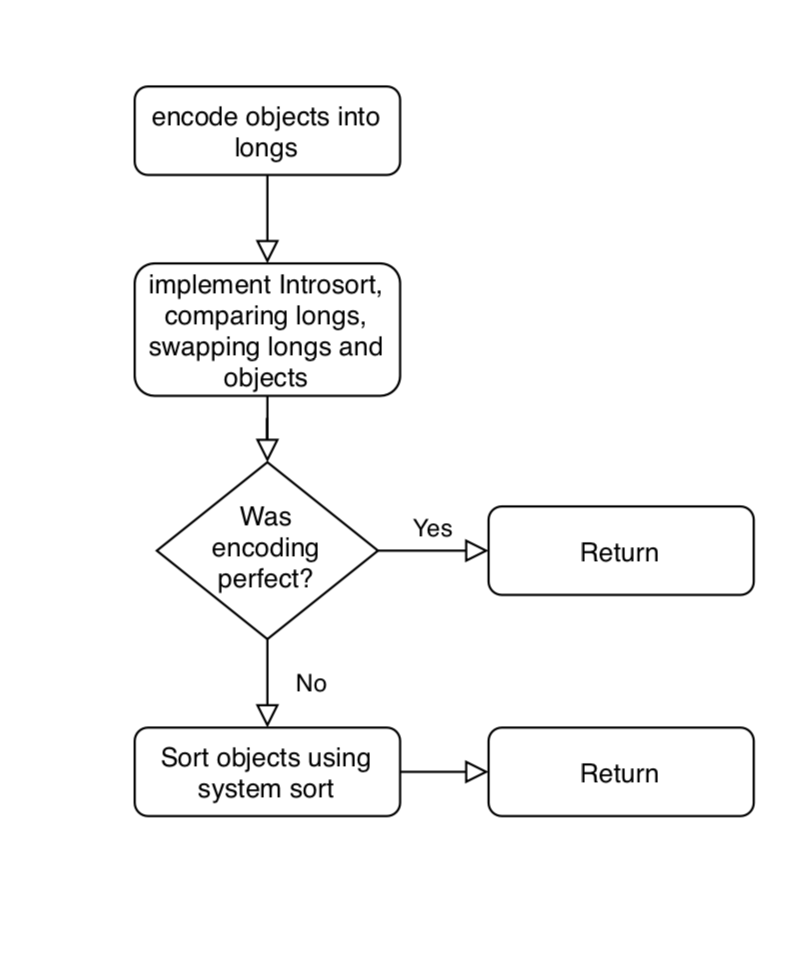
\includegraphics[trim=62 74 22 38, clip, width=0.39\linewidth]{HuskySortFlow.png}
\end{figure}
The strategy of HuskySort (see Flow ~\ref{Fig:HS}) is as follows,
assuming the dataset is presented as an array $xs$ of type $X$:


\begin{steps}
\item  
\renewcommand{\labelenumi}{\alph{enumi}}
    \begin{enumerate}
    \item Create a $long[]$ array (\emph{longs}) of the same size as $xs$;
    \item for each element $x$ of $xs$, set the corresponding element of \emph{longs} to $x.huskyCode()$.
    \end{enumerate}
\item {}Sort array \emph{longs} using quicksort (in practice, we have found that Introsort\cite{doi:10.1002} works well)
in such a way that when elements $i, j$ of \emph{longs} are exchanged, then elements $i, j$ of $xs$ are also exchanged;
\item {}Finally, when quicksort is finished and, if necessary,
we run Timsort on the array $xs$ to ensure that its elements are truly in order.
\end{steps}

For a worked example of a husky coding, see Algorithm ~\ref{alg:permitcoder}

\subsection{RadixHuskySort.}
\label{sec:radix}

Step 2 sorts the husky codes using Introsort, an $\textbf{O}(N log N)$ algorithm,
but the codes themselves are fixed-width 64-bit values,
and radix sort can sort $k$-bit keys in $\textbf{O}(N \cdot \frac{k}{b})$ time using $b$-bit digits —
linear in $N$ for any fixed digit width $b$.
Given that HuskySort's entire premise is to move work from the linearithmic phase to the linear phase,
this raises a natural question we had not previously addressed:
could step 2 itself be made linear? This section describes RadixHuskySort, which we built to answer it (Algorithm ~\ref{alg:the_alg5}).

Radix sort's linear-time advantage rests on a further assumption beyond fixed key width:
that a digit can be turned into an array index in $\textbf{O}(1)$ time,
so that counting and scattering never need to compare two digits directly.
A $b$-bit digit of a husky code satisfies this trivially —
it is extracted by a single shift and mask, and used directly as an index into a $2^b$-bucket counting array.
The original \textit{Comparable} type generally does not:
without first reducing it to such a code, radix sort applied directly to a \textit{String},
a \textit{Tuple}, or a case class would need some other way to decide which of $2^b$ buckets a given key belongs to,
and whenever the natural notion of a "digit" for such a type is not already a small, dense integer,
that decision falls back to \textit{equals} (and, for a hash-based bucket structure,
\textit{hashCode}) on the type itself — an $\textbf{O}(\text{size of the value})$ operation, not an $\textbf{O}(1)$ one.
Husky encoding is what removes this cost from every one of RadixHuskySort's $\frac{64}{b}$ digit passes,
not merely from the final comparison:
once the one-time $\textbf{O}(N)$ encoding step has run,
\textit{equals} and \textit{hashCode} on the original type are not called again until the optional cleanup pass.

A naive adaptation — swapping the object reference alongside each long at every exchange within every digit pass,
exactly as step 2's Introsort swaps at every partition exchange —
would incur $\textbf{O}(N)$ reference movements per digit pass, or $\textbf{O}(N \cdot \frac{64}{b})$ movements in total.
Since $\frac{64}{b}$ is typically much smaller than $log N$ at the sizes we tested,
this would still usually beat Introsort's swap cost,
but it needlessly reintroduces exactly the kind of payload-movement overhead this whole design exists to avoid,
and least-significant-digit (LSD) radix sort's per-pass counting-sort structure makes a better option available.

Instead, RadixHuskySort's step 2 carries only an $\textit{int[]}$ index array through the LSD digit passes,
alongside the (unmodified) long array;
each pass is a stable counting sort keyed on one $b$-bit digit of the (already-computed) husky code,
reordering the index array rather than the codes or the objects themselves.
Once all $\frac{64}{b}$ passes are complete, the index array holds the sorting permutation,
and a single $\textbf{O}(N)$ pass builds the final object array by reading $\textit{xs[index[i]]}$ for each $i$.
This confines all object-reference movement to one pass total, rather than one pass per digit.

Because LSD radix sort's per-digit counting sort treats keys as unsigned,
and husky codes are signed 64-bit values whenever the underlying domain can be negative (e.g., \textit{Integer},
\textit{Long}, or dates before a chosen epoch), each code is first transformed by $\textit{code} \oplus \textit{Long.MIN\_VALUE}$ —
flipping only the sign bit — before the digit passes,
which places negative codes before non-negative ones under unsigned digit comparison without disturbing relative order within either group;
the same transform is idempotent to reverse, so no separate un-flip step is needed once the permutation is built from the transformed codes.
Whether a given \textit{HuskyCoder} can actually produce negative codes is checked rather than assumed,
since several codings (e.g., Unicode strings) never do.

The digit width $b$ is a tunable parameter, trading off the number of passes ($\frac{64}{b}$)
against the size of the per-pass counting array ($2^b$ buckets, which must fit comfortably in cache for each pass to stay fast);
\S~\ref{sec:radix-results} reports how this trade-off plays out empirically across data types and array sizes.
Step 3 (the cleanup pass, run only if the coding is not provably \textit{perfect})
is unchanged regardless of which algorithm sorts the codes in step 2 —
radix sort is a drop-in replacement for that one step, not a change to the overall three-step strategy.

This parameterization also addresses a related limitation:
assuming 64-bit words throughout may not be appropriate for comparison on different key sizes.
Quicksort's asymptotic behaviour does not depend on key width at all —
an $\textbf{O}(N \log N)$ comparison sort costs the same whether the keys being compared are 32 bits or 128 bits wide,
since only the (fixed-cost) comparison itself touches the key's actual bits.
Radix sort, by contrast, makes the key width an explicit, first-class parameter:
a $k$-bit key simply takes $\frac{k}{b}$ passes instead of $\frac{64}{b}$, with no change to the algorithm itself.
So while nothing about the discussion above depends on 64-bit words specifically,
the RadixHuskySort generalizes to other key widths more directly than a comparison-based sort does —
if a future encoding needed, say, 128 bits to capture more of an object's structure,
the same radix sort would apply unchanged, merely with twice as many passes.

Radix sort applied to strings specifically has its own substantial, and older, literature,
distinct from the general fixed-width-key radix sort described above.
Three-way radix quicksort (also called multikey quicksort) and MSD (most-significant-digit)
radix sort for strings were both popularized by Bentley and Sedgewick's classic treatment\cite{314161.314321},
and burstsort\cite{1064546.1180622} improves cache behaviour further by building a small trie to bucket strings before sorting.
These string-specialized algorithms sort variable-length strings directly, character by character, without a separate fixed-width encoding step.
RadixHuskySort's contribution is different in kind, not degree:
it is not a string-sorting algorithm, but a general mechanism applicable to any \textit{Comparable} type
with a 64-bit husky encoding (strings among them),
at the cost of the encoding's own fixed capture window (\S~\ref{sec:pcrit} above)
and a fallback cleanup pass whenever that encoding is imperfect.

That framing carries a consequence which Table ~\ref{tab:RadixImprovements} bears out,
and which we state rather than leave to be noticed:
the string rows of that table are its most variable by a wide margin.
They span from 3.4x down to 1.6x, nearly the whole of its range below dates,
where every other row falls between 2.1x and 3.6x.
Three factors account for the spread, and they compose.
The advantage grows with the cost of the type's native comparison, since that is what the encoding replaces;
it grows with the perfection of the encoding, since an imperfect one is paid for by the cleanup pass;
and it shrinks in the presence of algorithms specialised to the type.
Dates are the favourable extreme on all three counts --- a provably perfect coding, no cleanup pass at all,
and no specialised competitor --- and yield the largest margin in the table at 5.9x.
The string rows show those same three factors varying \emph{within} a single data type,
which is the more instructive demonstration.
Chinese words are favourable on the first two counts --- an expensive Unicode comparison,
captured well enough by the encoding --- and sit fourth of eleven, above all but three of the non-string rows.
Chinese personal names are unfavourable on the second: the comparison is more expensive still,
a table lookup per character, but the pinyin coding captures far less of the key than the Unicode
coding does, so ties are common and the cleanup pass does real work rather than none
(\S~\ref{sec:chinese-coders} accounts for the difference).
The more expensive comparison is paired with the weaker encoding, and this is the weakest result we report.
English words are unremarkable on the first two counts and distinctive on the third,
being the one case in this paper with a mature specialised literature ranged against it.

Strings are unfavourable on the third count in a way no other type in this paper is.
Half a century of specialised string sorting exists,
and a general mechanism should not be expected to beat it on its own ground.
We compared RadixHuskySort against both of the classic string sorts named above,
under JMH, on English and Chinese text, in code-point order so that every sort compared
performs the same task.
Both baselines are our own implementations,
each tuned so that its fallback below the partitioning cutoff allocates nothing
and compares from the depth the partitioning has already established.
Against three-way radix quicksort RadixHuskySort is faster at every size tested,
by 1.3--2.4x on English words and 3.1--4.0x on Chinese words,
with non-overlapping 99.9\% confidence intervals throughout.
Against MSD radix sort the result goes the other way at scale, though not by much:
on English text the two are indistinguishable at $N=32{,}000$,
and MSD is faster by 1.20x at $N=200{,}000$ and by 1.06x at $N=1{,}000{,}000$.
The advantage at $N=200{,}000$ is the robust one.
At $N=1{,}000{,}000$ three runs on the machine of record give 1.00x, 1.05x and 1.06x,
so at the largest size we measure the two algorithms are level to within the spread between runs,
and the direction should be read from the middle size rather than the largest.
We give this result because it locates the boundary rather than obscuring it.
MSD earns it on a corpus that suits it and within limits that are its own:
our implementation indexes an alphabet of 256 characters beyond ASCII,
which English text fits and neither Chinese corpus does,
and it offers no pinyin ordering,
so there is no MSD row for either Chinese corpus.
RadixHuskySort reaches every corpus in this paper through one encoding,
with no per-alphabet provision and no per-type implementation.
That is the claim being made, and the English result bounds it without contradicting it.
A direct empirical comparison against burstsort remains future work;
it is a trie-based, cache-conscious algorithm designed to beat both baselines used here on exactly this workload,
and we have not implemented it.

Code-point order is not a meaningful comparison for Chinese personal names specifically —
it is simply the wrong order for that use case, not merely a different one.
Leaving the word corpus in that order is deliberate: a directory of people has one conventional
ordering and it is by pinyin, where a word list has several --- by radical, stroke count, pinyin or
frequency, according to purpose --- so no single ordering is the right one to hold it to,
and code-point order keeps that row comparable with the English one.
A fair comparison for the names requires a pinyin-aware MultikeyQuicksort.
We extended it with the same syllable-then-tone character key the pinyin encoding of \S~\ref{sec:radix} already uses,
restricted the comparison to the three pinyin-aware sorters, and re-ran it.
RHSort is faster than the repaired multikey quicksort by 1.57x, 1.83x and 2.09x at $N = 32{,}000$,
$200{,}000$ and $1{,}000{,}000$, and QuickHuskySort by 1.33x, 1.49x and 1.27x.
Two independent runs on the machine of record agree to within two hundredths of those multipliers.
Note that the RHSort margin grows with $N$ while QuickHuskySort's does not:
the linear second phase keeps paying as the array grows where a linearithmic one cannot,
which is the same pattern the natural-order corpora show and the clearest form in which this corpus
shows it.

\begin{algorithm2e}
\KwIn{\it{xs} as an array of object X which extends Comparable<X>}
\KwIn{\it{b} as the number of bits per digit}
 coding = huskyCoder.huskyEncode(xs)\;
 longs = coding.longs\;
 index = radixSortIndices(longs, b)\;
 ys = permute(xs, index)\;
 \If{coding.perfect}{return ys\;}
 Arrays.sort(ys)\;
 \caption{RadixHuskySort.sort}
 \label{alg:the_alg5}
\end{algorithm2e}

\begin{algorithm2e}
\KwIn{\it{longs} as an array of long}
\KwIn{\it{b} as the number of bits per digit}
\KwOut{\it{index}, a permutation of $0, \ldots, \textit{longs.length} - 1$ such that
  \textit{longs[index[$\cdot$]]} is sorted}
 biased[i] = longs[i] {\bf XOR} Long.MIN\_VALUE, for each i\;
 index = [0, 1, \ldots, longs.length - 1]\;
 \For{digit = 0 \KwTo (64 / b) - 1}{
 index = stableCountingSortPass(biased, index, digit, b)\;
 }
 \caption{radixSortIndices (LSD, deferred permutation)}
 \label{alg:the_alg6}
\end{algorithm2e}

\subsection{Discussion of Husky Encoding.}

Step 1b requires the definition of a 64-bit hash function (huskyCode) whose properties are as follows:
(refer to Algorithm ~\ref{alg:the_alg2})
\begin{itemize}
                        \item {}If $x = y$, then $x.huskyCode() = y.huskyCode()$;
                        \item {}If $x > y$, then: 
                            \begin{itemize}
                            \item{} either $x.huskyCode() <= y.huskyCode()$ (with probability $p$)
                            \item{} or $x.huskyCode() > y.huskyCode()$ (with probability $1-p$);
                            
                            \end{itemize}
                        
                        \end{itemize}


We interpret this rule as follows:
if $x$ and $y$ are the same ($x.equals(y)$ in Java), their huskyCode should be the same.
If $x > y$, we normally expect that $x.huskyCode() > y.huskyCode()$, i.e., the sort on the husky-coded longs will not invert $x$ and $y$.
However, when $x > y$ while $x.huskyCode() < y.huskyCode()$, then an inversion will be introduced.
And, when $x > y$ and $x.huskyCode() = y.huskyCode()$, then an inversion \emph{may} be introduced because quick-sort is not stable.\cite{6115063}

For a successful encoding, the value of $p$, the probability of a potential inversion, should be less than some critical probability, $p_{crit}$.
Leaving a more detailed discussion of $p_{crit}$ until later, we note that, for some domains of $X$, we can definitely assert that $p = 0$.
We refer to this as a “perfect” encoding.
In such a case, we can skip step 3 of the algorithm because, when $p = 0$, there will be no inversions remaining after quick-sorting according to the huskyCodes.
An example of such a domain is date-time values with a resolution of one nano-second over a period of 128 years.
For strings of English case-independent letters (no punctuation or numbers), i.e., 5-bit ASCII, words of 12 (or fewer) characters in length can also be coded uniquely.
For case-dependent strings (6-bit ASCII), we can encode perfectly if the lengths are all 10 characters or less.
In step 3, it might be acceptable to use insertion sort instead of Timsort.
In any event, assuming that the huskyCode is as accurate as required, then there will be very few inversions (elements out of place) remaining after the quicksort phase.
This implies that the second sort can be performed in very close to linear time.
The results have been very satisfactory.
For example, taking an array of 1,000,000 English words drawn randomly from a corpus of 275,333\cite{GOLDHAHN12.327},
QuickHuskySort sorts in 698 ms against the system sort's 1,121 ms, a factor of 1.61
(for the full data, please refer to table ~\ref{tab:HS_BM}).






\subsection{Discussion of \texorpdfstring{$p_{crit}$}{p\_crit}.}
\label{sec:pcrit}
When $p > 0$, there is a finite probability of any pair of elements remaining inverted after the first sorting pass.
For an array of N randomly ordered elements, the average number of inversions before sorting is $X = N (N -1 ) / 4$.
The number of inversions remaining after the first pass is simply $p X$.
And, for Timsort or insertion sort, the time to re-sort the array will be $t = k (N + p X)$ where $k$ is some system-dependent constant.
The total time to sort the array is made up of these three time-consuming steps where $k_1, k_2, k_3$ are system- and algorithm-dependent constants:

\begin{steps}
 \item{} $T_1$ is the time to encode the elements:
\[T_1 = k_1 N\]
\item{}  $T_2$ is the (average) time to quick-sort the huskyCode array while also swapping the element array itself:
\[T_2 = 2 k_2 N ln N\]
\item{}  $T_3$  is the time to Timsort the element array (only required if $p>0$):
 \[T_3 = k_3 (N + p X)\]
\end{steps}
Provided that the total time $T = T_1 + T_2 + T_3$ is less than the time required to use Timsort on the original element array, we have a win.
This same three-step decomposition ($T_1$/$T_2$/$T_3$, i.e., encode/sort/cleanup) is revisited in \S~\ref{sec:analysis}
in more concrete terms —
counting array accesses directly rather than folding everything into abstract system-dependent constants $k_1, k_2, k_3$ —
and extended there to cover RadixHuskySort (\S~\ref{sec:radix}) as a fourth alternative for the $T_2$ step.
The actual values of $p_{crit}$ are very much dependent on the machine running the sort.
We have not calculated a typical value for $p_{crit}$ but, even for the worst-case:
Chinese characters using UTF8 encoding, we still find very significant gains, reported later in Table ~\ref{tab:HS_BM}.

Of the three terms, $T_3$ can be isolated experimentally.
Two benchmarks over the same two hundred thousand municipal records (\S~\ref{sec:radix-results})
differ only in which coder they are given.
Both compute identical codes; one coder declares itself perfect, so the sort skips step 3,
while the other leaves that declaration at its default and the pass runs.
The encoding for these records is perfect, so the pass that runs has provably nothing to correct.

Its cost is predictable in advance.
Timsort over a fully ascending array detects a single run and stops,
performing $N-1$ comparisons and no moves,
so $T_3$ at $p = 0$ is exactly $N-1$ invocations of the element's own comparator ---
here assessor's block, then lot, then filing date,
which is precisely the comparison the husky encoding was introduced to avoid.
The cleanup pass reintroduces one full composite comparison per element,
having just removed it from all $\textbf{O}(N \log N)$ of them.

That comparison costs 16.1\,ns at $N = 32{,}000$, 60.3\,ns at $N = 100{,}000$ and 74.2\,ns at
$N = 198{,}900$ --- 7.3\%, 17.2\% and 17.3\% of the running time of the sort that contains it ---
with non-overlapping 99.9\% confidence intervals throughout.
Three further runs, one of them on different hardware, agree on the shape at different levels;
across all four the pass costs between a sixteenth and a quarter of the total,
and between a sixth and a quarter at the two larger sizes.
The percentages are the less stable figures, being ratios of two quantities that both move.
The shape is a threshold rather than a trend --- a rise by a factor of roughly three to four between the first two sizes,
then a levelling off --- and it falls where the records stop fitting in cache.
That last reading is inference, but the magnitudes support it:
the system sort compares these same records some 3.5 million times in 151\,ms, or 43\,ns each,
so the cleanup pass at 74\,ns costs nearly twice as much per comparison using the same comparator.
Step 2 permutes references without moving the records,
so a scan sequential in the array is close to random in the heap.

Whether this share must shrink as $N$ grows --- the pass being linear where the sort containing it is
linearithmic --- is a fair question, and \S~\ref{sec:cleanup-scaling} answers it.

Two conclusions follow.
First, $k_3$ is not a constant: it varies more than fourfold across three sizes on one machine,
so no single $p_{crit}$ can be quoted even for one type on one machine.
Second, an encoding which can be declared perfect avoids a cost of up to a quarter of total running
time, where one which cannot must repay it before correcting a single genuine inversion.

\subsection{Why husky coding works.}
\label{sec:why-husky}

The rationale is set out in full by Hillyard et al.\cite{huskysort2020}; we restate only what the rest of
this paper depends on.
A 64-bit word holds enough of most keys to place elements close to their final order, and comparing two
longs costs far less than following two object references and running a type-specific
\textit{compareTo} --- so the encoding trades one $\textbf{O}(N)$ pass for cheaper comparisons throughout
the $\textbf{O}(N \log N)$ one.
The code need not be perfect, only good: whatever inversions it leaves are the cleanup pass's problem, and
\S~\ref{sec:pcrit} measures what they cost.

Perfection has a precise limit for strings.
Packing four 16-bit characters fills the word (Table ~\ref{tab:EncodingConstants} gives the constants for
both string codings), but the packed result is then shifted right by one bit, because any string whose
first character is \texttt{0x8000} or above --- common among CJK characters --- would otherwise set the
sign bit and encode as a negative \textit{long}, corrupting numeric comparison.
The shift costs the least significant bit of a true fourth character; for three characters or fewer that
bit is padding, which is why the Unicode coding is declared \textit{perfect} up to three characters and
not four.

Whether a coding was in fact perfect is known before the cleanup pass runs: a constant-time lookup for
non-sequence types, and for strings a scan that stops at the first string too long to encode perfectly.
Where it was perfect, no inversions remain and the pass is skipped altogether.


\begin{algorithm2e}
\KwIn{\it{xs} as an array of object X}
\KwOut{A new \it{Coding} object}
 result = new long[xs.length]\;
 \For{i = 0 to xs.length}{
 result[i] = huskyEncode(xs[i])\;
 }
 return new Coding(result, perfect())\;
 \caption{huskyEncode}
 \label{alg:the_alg2}
\end{algorithm2e}


\begin{algorithm2e}
\KwIn{\it{permit}, with fields \it{block}, \it{lot}, \it{filedDate}\;}
\KwOut{a 60-bit code, order-preserving for \it{permit.compareTo}}
 \tcp{fields most-significant first, in compareTo order}
 r = encodeString(block, 5, 5, BLOCK\_ALPHABET)\;
 r = r $\ll$ 24 $|$ encodeString(lot, 4, 6, LOT\_ALPHABET)\;
 \Return r $\ll$ 11 $|$ daysSinceEpoch(filedDate)\;
 \BlankLine
 \tcp{codeOf(x, alphabet), used by encodeString for each symbol}
 \eIf{alphabet contains x}{
   \Return 1 + index of x\tcp*{0 is left for padding}
 }{
   \Return count of symbols $<$ x\tcp*{weaken, never invert}
 }
 \caption{A composite husky coder: \textit{PermitCoder}. \textit{encodeString} packs \textit{width}
   symbols of \textit{bits} each, right-padding with zero.}
 \label{alg:permitcoder}
\end{algorithm2e}

\section{Implementation.}

%% ANONYMISATION: the real URL names its owner, so it is guarded with the author block. See
%% "0i. The repository link" in Paper edits pending.md -- the Anonymous GitHub mirror is task 2
%% on Sai Vineeth's list; when its URL exists, substitute it for the placeholder below and the
%% review copy can cite the code directly.
\ifanonymous
  The implementation is available in an anonymised repository, linked from the submission site.
\else
  The implementation is available at \url{https://github.com/rchillyard/HuskySort}.
\fi

\subsection{System Environment.}

Three machines appear in this paper, and \S~\ref{sec:environments} specifies all three.
Machine A ran the JDK 1.8.0\_152 comparison-sort benchmarks of \S~\ref{sec:analysis},
the choice of cleanup sort among them (\S~\ref{sec:cleanup-choice});
machine B, on different hardware and two JVM generations later, ran the radix-sort and JMH development work.
Machine C is the machine of record: an independently administered cloud instance, confirmed idle before
each run, and the source of every figure quoted in this paper.
It is ARM-based like machine B but differs from it in core design, vendor, core count and operating system.

Reporting all three lets a reader check directly whether the qualitative finding generalizes across
machines and JVM versions rather than being an artifact of one environment.
It does: QuickHuskySort, and now RHSort, beat the system sort on all three,
which differ in vendor, instruction set, core design and JVM generation.



\begin{table}
  \caption{String-encoding constants}
  \label{tab:EncodingConstants}
  \begin{tabular}{lll}
    \toprule
    Constant & Unicode & ASCII \\
    \midrule
    Bit width per character & 16 & 7 \\
    Max length (64 / bit width) & 4 & 9 \\
    Mask & \texttt{0xFFFF} & \texttt{0x7F} \\
    \bottomrule
  \end{tabular}
\end{table}

\section{Test Case and Analysis.}

\subsection{Data Source.}
\label{sec:data-source}
The sources for the Strings (English and  Chinese) are retrieved from Leipzig Corpora Collection\cite{GOLDHAHN12.327}.
Chinese personal names, used for the pinyin-order comparisons of \S~\ref{sec:radix-results}, are a separate corpus\cite{wainshine2020chinesenames}.
Every other dataset in this paper is generated: pseudo-random numbers, dates and tuples.
The building-permit records of \S~\ref{sec:radix-results} are not.
They are 198,900 permits filed between January 2013 and February 2018, taken from San Francisco's published
record\cite{sf-building-permits} and ordered by a composite key of assessor's block, lot and filing
date; they are included because their distribution is the city's rather than ours.
Only those three columns are retained, and the data is used under the Open Data Commons Database
Contents License.

In each case, we take data from the appropriate \emph{sentences.txt} file and break it up into strings as shown in Listing~\ref{lst:DS}.


\begin{lstlisting}[caption={Data Source},label={lst:DS},language=Java]
private static String[] getLeipzigWordsFromResource(final String resource) {
    return getWords(resource, HuskySortBenchmark::getLeipzigWords);
}
private static List<String> getLeipzigWords(final String line) {
    return HuskySortBenchmarkHelper.splitLineIntoStrings(line, REGEX_LEIPZIG, REGEX_STRINGSPLITTER);
}
final static Pattern REGEX_LEIPZIG = Pattern.compile("[~\\t]*\\t(([\\s\\p{Punct}\\uFF0C]*\\p{L}+)*)");
public static final Pattern REGEX_STRINGSPLITTER = Pattern.compile("[\\s\\p{Punct}\\uFF0C]");


static List<String> splitLineIntoStrings(final String line, final Pattern lineMatcher, final Pattern stringsplitter) {
    final Matcher matcher = lineMatcher.matcher(line);
    if (matcher.find()) return Arrays.asList(stringsplitter.split(matcher.group(1)));
    else return new ArrayList<>();
}

static String[] getWords(final String resource, final Function<String, List<String>> stringListFunction) {
    try {
        File file = new File(getPathname(resource, DutchHuskySort.class));
        return getWordArray(file, stringListFunction, 2);
    } catch (FileNotFoundException e) {
        logger.warn("Cannot find resource: "+resource, e);
        return new String[0];
    }
}
    } catch (final Exception e) {
        throw new RuntimeException(e);
    }
}


\end{lstlisting}

\subsection{Analysis.}
\label{sec:analysis}
Let’s try to do an analysis of QuickHuskySort's performance.
This expands on the $T_1$/$T_2$/$T_3$ decomposition introduced in \S~\ref{sec:pcrit} above,
replacing its abstract time constants with concrete array-access counts,
and extending it to cover RHSort (\S~\ref{sec:radix}) as an alternative to quicksort for the $T_2$ step.
The first thing to note is that, like merge sort, QuickHuskySort requires $\textbf{O}(N)$ extra space.
This is because, in addition to the array of object references, we must have an equal-length array of longs (the huskyCode values).

Secondly, QuickHuskySort is not stable unless using the merge sort variation.
The derivation of the two comparison figures is a counting argument rather than a measurement, and it
rests on one coefficient we estimated rather than measured; it is set out in \S~\ref{sec:qhs-analysis}.

Encoding's cost has not simply been assumed:
we timed the encoding phase in isolation,
separately from the sort that follows it, to confirm it directly.
At $N = 1{,}000{,}000$, encoding takes 67.7ms for English words (9.7\% of QuickHuskySort's 697.9ms total,
24.8\% of RHSort's 272.7ms) and 211.1ms for Chinese names encoded via pinyin (16.9\% of QuickHuskySort's
1252.7ms, 27.8\% of RHSort's 760.9ms) — confirming that encoding cost, while real and non-negligible,
especially for the more elaborate pinyin encoding, remains a minority of total time in every case measured,
consistent with the linear-and-subordinate role it is assumed to play above.
Encoding's share of the total is larger for RadixHuskySort than for QuickHuskySort in both cases,
simply because RHSort's own contribution to the total is smaller —
as the sort phase gets cheaper,
whatever cost remains in the encoding phase necessarily becomes a proportionally larger slice of what is left,
which suggests encoding cost (particularly for pinyin)
is the more promising target for further optimization now that the sort phase itself is no longer the dominant cost.
The consequence of this is that, as expected,
the linear phase of QuickHuskySort is relatively high for small $N$ but that is soon swamped by the saving of comparisons in the linearithmic phase.
The break-even point is actually a very small value of $N$:
four.
As $N$ increases, we expect the advantage of QuickHuskySort to increase further.
This is generally borne out by the benchmarks.
Please refer to table ~\ref{tab:Comparison}.

The same style of analysis extends naturally to RadixHuskySort (\S~\ref{sec:radix}).
Each of its $\frac{64}{b}$ digit passes touches every element a small constant number of times,
$c$, to bucket it and to record its new position in the (deferred) index array —
with no partitioning or pivot-comparison overhead, and critically, no logarithmic term at all.
Taking $c = 4$ (the same per-exchange cost used for QuickHuskySort's swaps above),
adding the final $\textbf{O}(N)$ pass that applies the resulting permutation to the object array (2 array accesses per element),
and the same encoding cost ($(k+1)N$) and cleanup-pass cost ($(2 + j + 4)pN$,
unaffected by which algorithm sorts the codes in step 2), the total array accesses for RadixHuskySort ($A_r$) come to:
\[A_r = \left(4 \cdot \frac{64}{b} + 2 + k + 1\right) N + (2 + j + 4)pN\]
Using the same illustrative constants as above ($j = 4$, $k = 7$, $p = 0.1$)
and $b = 16$ (four digit passes, near the middle of the digit-width plateau found empirically —
see \S~\ref{sec:radix-results}):
\[A_r = 27 N\]
Table ~\ref{tab:Comparison} extends the earlier comparison with this term.
At $N = 1{,}000{,}000$, $A_r \approx 27{,}000{,}000$ against $A_h \approx 101{,}000{,}000$ and $A_m \approx 161{,}000{,}000$ —
a predicted advantage of roughly 3.7x over QuickHuskySort,
consistent with the 2-4x speedups actually measured (\S~\ref{sec:radix-results}).
The model does predict one caveat:
equating $A_r$ and $A_h$ gives a theoretical break-even around $N \approx 17$,
somewhat higher than QuickHuskySort's own break-even against merge sort ($N = 4$,
above) — because RHSort's per-pass cost has no logarithmic term to shrink relative to at very small $N$.
This crossover is far below every array size actually tested, so it has no practical effect on the results reported here,
but it is worth stating rather than leaving the model looking like radix wins unconditionally at every $N$.
 \begin{table*}
  \caption{Theoretical comparisons (array accesses, dimensionless counts)}
  \label{tab:Comparison}
  \begin{tabular}{rrrrr}
    \toprule
    N  &  N ln N & merge sort & QuickHuskySort & RHSort \\
    \midrule
     4 & 6 & 72 & 72 & 108 \\
     1,000 & 6,908 & 81,439 & 55,075 & 27,000 \\
     1,000,000 & 13,815,511 & 160,878,371 & 101,149,455 & 27,000,000 \\
     1,000,000,000 & 20,723,265,837 & 240,317,557,125 & 147,224,183,132 & 27,000,000,000 \\

    \bottomrule
  \end{tabular}
\end{table*}

Since the final pass of HuskySort will be cleaning up a relatively small number of inversions, does it
matter whether we use insertion sort or Timsort?
Below about 50,000 Strings it makes barely any difference, and insertion sort is sometimes faster;
beyond that Timsort wins out, by a factor of four and a half at $N = 4{,}000{,}000$.
That measurement, and the choice it settles, are in \S~\ref{sec:cleanup-choice}.


\section{Results and Observations.}
\subsection{Benchmarks.}

Table ~\ref{tab:HS_BM} reports absolute sort times for every data type and corpus.
The two radix columns bracket the digit-width plateau of \S~\ref{sec:radix-results}.
Dual-pivot quicksort and a from-scratch quicksort were measured too; they bear on QuickHuskySort
rather than on RHSort, so they are in \S~\ref{sec:comparison-baselines}.

\begin{table*}
  \caption{Sort times by data type (JMH, ms, mean $\pm$ 99.9\% CI). Numeric types at $N=500{,}000$.
    For Chinese names the system-sort column is a system sort performing the same pinyin ordering;
    code-point order is a different and much cheaper task (\S~\ref{sec:radix-results}).}
  \label{tab:HS_BM}
  \begin{tabular}{llllll}
    \toprule
    Data type & N & System sort & QuickHuskySort & RHSort/8 & RHSort/16 \\
    \midrule
    Integer & 500,000 & 121.2$\pm$0.6 & 89.7$\pm$3.5 & 31.2$\pm$0.5 & 25.2$\pm$0.2 \\
    Double & 500,000 & 141.7$\pm$1.3 & 97.8$\pm$3.6 & 34.0$\pm$0.5 & 31.0$\pm$0.3 \\
    Long & 500,000 & 135.8$\pm$1.2 & 97.7$\pm$1.0 & 30.2$\pm$0.2 & 28.6$\pm$0.3 \\
    BigInteger & 500,000 & 208.4$\pm$1.7 & 152.3$\pm$1.7 & 56.9$\pm$0.3 & 54.1$\pm$0.2 \\
    BigDecimal & 500,000 & 262.2$\pm$1.6 & 144.1$\pm$2.1 & 54.1$\pm$0.3 & 52.5$\pm$0.3 \\
    English words & 32,000 & 13.69$\pm$0.19 & 9.72$\pm$0.12 & 4.63$\pm$0.16 & 4.18$\pm$0.16 \\
    & 200,000 & 141.39$\pm$2.59 & 94.74$\pm$2.44 & 55.01$\pm$2.20 & 50.27$\pm$2.51 \\
    & 1,000,000 & 1120.87$\pm$14.43 & 697.88$\pm$16.15 & 355.26$\pm$24.71 & 272.74$\pm$6.46 \\
    Chinese words & 32,000 & 9.78$\pm$0.08 & 5.00$\pm$0.04 & 2.10$\pm$0.03 & 1.89$\pm$0.02 \\
    (code-point order) & 200,000 & 71.34$\pm$0.63 & 30.90$\pm$0.13 & 13.49$\pm$0.15 & 10.85$\pm$0.10 \\
    & 1,000,000 & 447.12$\pm$2.28 & 219.80$\pm$1.99 & 83.25$\pm$2.31 & 65.46$\pm$1.47 \\
    Chinese names & 32,000 & 69.1$\pm$1.4 & 26.6$\pm$0.3 & 24.1$\pm$0.2 & 23.1$\pm$0.3 \\
    (pinyin order) & 200,000 & 526.2$\pm$9.5 & 187.2$\pm$1.0 & 157.0$\pm$1.3 & 154.9$\pm$1.2 \\
    & 1,000,000 & 3112.9$\pm$68.0 & 1252.7$\pm$6.4 & 775.7$\pm$4.2 & 767.2$\pm$14.0 \\
    Tuples & 20,000 & 3.72$\pm$0.01 & 2.79$\pm$0.02 & --- & 1.30$\pm$0.01 \\
    & 100,000 & 23.24$\pm$0.19 & 17.65$\pm$0.16 & --- & 6.82$\pm$0.05 \\
    & 500,000 & 209.53$\pm$7.98 & 142.61$\pm$1.83 & --- & 57.98$\pm$0.76 \\
    \bottomrule
  \end{tabular}
\end{table*}

\subsection{Summary.}
\label{sec:summary}
HuskySort’s target application is the sorting of randomly ordered arrays of objects on the JVM (Java Virtual Machine).
Let’s eliminate the non-use-cases first:
\begin{itemize}
\item {}Partially-ordered arrays:
that’s to say, arrays with only a linear number of inversions as would be the case when adding a relatively small number of records to a large existing index.
For such use cases, Timsort (the Java system sort for objects) would be more suitable.

\item {}Arrays of primitives:
in Java, a clear distinction exists between primitive types (char, byte, short, int, float, long, double) and objects.
Dual-pivot quicksort (the Java system sort for primitives) is already the fastest algorithm for sorting such types.
\end{itemize}
Thus, HuskySort is best for any object array where there’s no expectation of partial ordering.
Typical improvements over Timsort can be read directly off Table ~\ref{tab:HS_BM} above, which gives
absolute times with 99.9\% confidence intervals rather than summary ranges:
1.4--1.8x across the five numeric types at $N=500{,}000$,
1.4--1.6x on English words,
2.0--2.3x on Chinese words,
and 1.3--1.5x on tuples.
Note that the English margin \emph{widens} with array size rather than decaying,
from 1.41x at $N=32{,}000$ to 1.61x at $N=1{,}000{,}000$.

\subsection{Radix Sort Results.}
\label{sec:radix-results}

We benchmarked every data type and corpus covered above using RadixHuskySort (\S~\ref{sec:radix})
in place of Introsort for step 2, using JMH (the Java Microbenchmark Harness, with proper fork isolation and warmup) on JDK 21.

Table ~\ref{tab:RadixImprovements} reports RHSort's advantage over QuickHuskySort as a direct multiplier —
e.g., \textbf{2.9x} means radix took roughly a third as long —
rather than as a percentage, since a percentage figure close to or above 100\% becomes ambiguous about exactly which quantity it is a percentage \emph{of}.

\begin{table*}
  \caption{RHSort's advantage over QuickHuskySort, as a direct multiplier}
  \label{tab:RadixImprovements}
  \begin{tabular}{cll}
    \toprule
    Data Type & N & Advantage over QuickHuskySort \\
    \midrule
    \texttt{Dates} & 20,000 & 5.9x \\
    \texttt{Long} & 500,000 & 3.6x \\
    \texttt{Integer} & 500,000 & 3.6x \\
    \texttt{Strings of Chinese words (code-point order)} & 1,000,000 & 3.4x \\
    \texttt{Double} & 500,000 & 3.2x \\
    \texttt{BigInteger} & 500,000 & 2.8x \\
    \texttt{BigDecimal} & 500,000 & 2.8x \\
    \texttt{Strings of English words} & 1,000,000 & 2.6x \\
    \texttt{Tuples} & 500,000 & 2.5x \\
    \texttt{Building permits (composite key)} & 198,900 & 2.1x \\
    \texttt{Strings of Chinese names (pinyin order)} & 1,000,000 & 1.6x \\
    \bottomrule
  \end{tabular}
\end{table*}

This is worth confronting directly, since a reader might reasonably ask whether either advantage erodes
as $N$ grows: a constant-factor saving on a linearithmic sort could be swamped at scale.
Neither does.
QuickHuskySort's margin over the system sort on English text \emph{widens} with size,
from 1.41x at $N=32{,}000$ to 1.49x and then 1.61x (Table ~\ref{tab:HS_BM}),
and holds roughly constant on both Chinese corpora.
Radix sort's advantage over QuickHuskySort likewise does not shrink with $N$:
at every size and data type in Table ~\ref{tab:RadixImprovements}, the margin is 1.5x or greater,
consistent with the theoretical model of \S~\ref{sec:radix} predicting no logarithmic term at all,
so there is no analogous reason to expect the advantage to erode as $N$ grows further.
The spread across that table is itself informative, and follows the three factors of \S~\ref{sec:radix}.
Chinese names sorted by pinyin order are the smallest margin measured (1.6x),
because both QuickHuskySort and RadixHuskySort must pay the same cleanup pass for a coding
that two or three characters of recurring syllables leave badly imperfect.
Dates show the largest margin (5.9x) because that coding is provably perfect and never needs a cleanup pass at all,
letting RHSort's linear-time advantage show through with nothing else in the way.
The two lie at opposite ends of the same axis: what separates them is not the data type but the perfection of the encoding.

The building permits row is the only one in that table not measured on data we generated:
198,900 real municipal records ordered by a composite key of three fields (\S~\ref{sec:data-source}).
At 2.1x it is tenth of eleven, which is the point worth making about it --- it is not our largest
margin, but it is our largest on data whose distribution we did not choose.
\S~\ref{sec:permits} gives the case study, and \S~\ref{sec:composite-future} what a general
composite encoder would have to provide, that one having been written by hand.

The measurements were reproduced qualitatively on machines A and B of \S~\ref{sec:environments},
which differ from the machine of record and from each other in vendor, instruction set, core design and
JVM generation.
We quote no figures from them, since mixing environments within a comparison would rob it of meaning,
but every ordering reported here holds on all three.

\subsection{Parallel Radix Sort.}
\label{sec:parallel-radix}

Radix sort's digit passes are natural candidates for parallelization (\S~\ref{sec:radix} above).
We implemented and benchmarked a parallel variant:
each pass is split into a configurable number of contiguous chunks, one per worker thread.
Every chunk first computes its own local per-bucket histogram independently, with no synchronization required;
a short sequential step then combines those histograms into an exact starting offset, in the output array,
for every (chunk, bucket) pair — preserving the stability that step 3's cleanup pass, when needed, relies on,
since a chunk's elements always land after all lower-numbered chunks' elements sharing the same bucket;
finally, every chunk scatters its own elements into the output arrays independently,
using only its own precomputed offsets, so no two chunks ever write to the same location.

An initial implementation dispatched the two phases above to a thread pool separately on every pass.
Measurement showed this repeated dispatch itself contributing a real, non-trivial share of the total cost,
particularly at more moderate array sizes.
The overhead was substantially reduced by starting the worker threads once per sort,
rather than once per phase per pass:
each thread runs its own loop over every pass, and the two phases synchronize via reused barriers whose associated actions —
code that runs exactly once per synchronization point, in whichever thread arrives last —
perform the histogram-combine and buffer-swap steps.
Table ~\ref{tab:ParallelRadix} reports the result (\textit{Long[]}, 11-bit digits, milliseconds, mean $\pm$ 99.9\% CI).

\begin{table*}
  \caption{Parallel RHSort:
serial vs. 1, 2, 4, and 8 worker threads}
  \label{tab:ParallelRadix}
  \begin{tabular}{cccccc}
    \toprule
    N & Serial & 1 thread & 2 threads & 4 threads & 8 threads \\
    \midrule
    2,000,000 & 172.0$\pm$5.7 & 165.2$\pm$2.2 & 140.3$\pm$2.0 & 118.5$\pm$2.4 & 109.3$\pm$1.8 \\
    10,000,000 & 935.2$\pm$36.9 & 884.5$\pm$21.6 & 731.6$\pm$19.9 & 687.9$\pm$22.1 & 645.3$\pm$20.9 \\
    \bottomrule
  \end{tabular}
\end{table*}

Isolating parallelism itself, that's to say comparing 1 thread against 4, both paying identical thread-coordination overhead,
gives a statistically resolved speedup at both sizes: 1.39x at $N=2{,}000{,}000$ and 1.29x at $N=10{,}000{,}000$,
with non-overlapping confidence intervals in both cases.
Against the serial implementation the improvement is resolved at both sizes too,
172.0ms to 118.5ms at $N=2{,}000{,}000$ and 935.2ms to 687.9ms at $N=10{,}000{,}000$.
Unlike on the eight-core machine of an earlier draft, scaling does not stop at four threads:
on sixteen uniform cores, eight threads beats four at both sizes with intervals that do not overlap,
reaching 1.51x and 1.37x over a single thread.

That is still well short of linear, and the shortfall is the more interesting number:
an eightfold increase in threads buys between 1.4x and 1.5x,
on hardware with no performance/efficiency asymmetry to account for it.
Two explanations fit, and we cannot separate them without hardware counters.
Each digit pass scatters across the whole array, so the sort may simply be limited by memory throughput,
which extra cores do not supply; and each pass's histogram-combine step is sequential,
running once per synchronization point whatever the thread count,
so it grows as a share of the total as threads are added.
The first would be a property of the machine and the second of the design,
and only the second would survive better hardware.

\subsection{Use-Case Guidance.}
\label{sec:usecase}

\S~\ref{sec:summary} already eliminates two cases outright:
partially-ordered arrays, where Timsort's own adaptivity wins, and arrays of already-cheap-to-compare primitives,
where dual-pivot quicksort is already the fastest option.
For the remaining case — arrays of objects with no expectation of partial ordering —
the decision is governed by the three factors of \S~\ref{sec:radix}
rather than by the size of the array,
and Table ~\ref{tab:Guidance} puts them in the order a practitioner can answer them.
Size enters only once those are settled, and then only near the bottom of the range.

\begin{table*}
  \caption{Which sort to reach for. The situations are ordered by how much they decide, and
    array size settles nothing until all of them are.}
  \label{tab:Guidance}
  \begin{tabular}{p{0.42\textwidth}p{0.24\textwidth}p{0.26\textwidth}}
    \toprule
Your situation & Reach for & Evidence \\
    \midrule
    The ordering is already cheap to evaluate --- primitives, or a single numeric field
      & dual-pivot quicksort & cost of encoding cannot be recouped (\S~\ref{sec:summary}) \\
    The ordering is composite or expensive, \emph{and} the key packs exactly into 64 bits
      & RadixHuskySort; no cleanup pass is required
      & the largest margins we measure: dates 5.9x, building permits 2.1x over QuickHuskySort \\
    The ordering is composite or expensive, but the encoding is imperfect
      & RadixHuskySort, even allowing for the cleanup pass
      & that pass costs a sixth to a quarter past $N=100{,}000$, even with nothing to correct
        (\S~\ref{sec:pcrit}) \\
    A sort specialised to your type already exists
      & use it, if it covers your data
      & on English words a tuned MSD radix sort beats us, though our MSD indexes extended
        ASCII only and cannot sort either Chinese corpus (\S~\ref{sec:radix}) \\
    The data defeats the encoding's capture window --- long shared prefixes, or keys wider than
    the coder can see
      & System sort & every husky variant loses its advantage (\S~\ref{sec:adversarial}) \\
    None of the above settles it, or the keys are strings
      & by array size (\S~\ref{sec:usecase})
      & each sort's fixed setup cost is repaid at a different $N$ \\
    \bottomrule
  \end{tabular}
\end{table*}

Only when all of those are answered does array size matter, and then chiefly at the small end,
where each algorithm's fixed setup cost has not yet been amortized.
For String keys we measured every crossover directly (JMH, English corpus, $N=4$ through $10{,}000$).
System sort is the fastest of the group up to $N=20$, though only narrowly there
(0.462$\mu$s against insertion sort's 0.489$\mu$s).
A plain, binary-search-based insertion sort wins outright from $N=50$ through $N=200$ —
the one regime in this paper where plain insertion sort,
not either HuskySort variant, is the best available choice.
QuickHuskySort takes over between $N=200$ and $N=500$, and remains the best choice up to roughly $N=2{,}000$,
since RadixHuskySort's own fixed setup cost is not yet amortized below that point.
That cost can be read directly off the measurements: RadixHuskySort's time is a near-constant
166$\mu$s floor from $N=4$ to $N=500$, the allocation and initialisation of its counting structures,
which only the linear term begins to dominate past a few thousand elements.
Somewhere between $N=2{,}000$ and $N=10{,}000$ it takes over;
its advantage then grows and holds at every larger size tested (Table~\ref{tab:RadixImprovements}).
Every one of these crossovers shares the same shape:
each successive algorithm carries a larger fixed setup cost that only pays for itself once there is enough work to amortize it against —
the same fixed-vs-variable-cost story \S~\ref{sec:parallel-radix} found one level further down,
where ParallelRHSort's own thread/barrier setup only pays off once there is enough work to divide across threads.
These crossover points were measured only for String keys.
The fixed costs involved are architectural rather than type-specific,
so other key types plausibly show similarly-shaped curves at similar sizes,
though that has not been separately confirmed.

Two further caveats from elsewhere in this paper complete the picture.
If the source data defeats the husky encoding's fixed capture window entirely —
a shared prefix longer than the encoding's own character limit, for instance —
neither QuickHuskySort nor RadixHuskySort helps regardless of $N$ (\S~\ref{sec:adversarial}):
both lose to plain System sort, since the encoding pass becomes pure waste and the mandatory cleanup pass must do all the real work anyway.
And given a large enough workload and spare cores, \textit{ParallelRadixHuskySort}
widens RadixHuskySort's own advantage further still (\S~\ref{sec:parallel-radix}),
provided there is enough total work to amortize its own thread-coordination cost.

\section{Conclusion.}

The original idea behind HuskySort, that's to say QuickHuskySort,
was to shift work from the linearithmic phase of sorting to the linear phase (both the prelude and the postlude)
and effect an overall reduction in array accesses and thus processing time.
\label{sec:conclusion-dp}%
This has been demonstrated such that, when sorting objects rather than primitives,
HuskySort is faster than dual-pivot quicksort wherever the ordering is expensive to evaluate ---
by 1.4x on \textit{BigInteger} and 1.7x on \textit{BigDecimal} (\S~\ref{sec:comparison-baselines}).
On \textit{Integer}, \textit{Double} and \textit{Long}, where a comparison costs almost nothing,
the encoding has nothing to amortise and dual-pivot quicksort is ahead instead, by up to a tenth.
That is the same criterion which governs every other result in this paper,
here separating one group of numeric types from another.
It is faster than Timsort for arrays which are not partially ordered, above a few hundred elements;
below that, Timsort's own tuned handling of small arrays wins instead.
It is especially fast for types whose ordering is composite or expensive to evaluate
and whose keys encode perfectly, where the encoding replaces the whole comparison and no cleanup pass is needed.
Strings are not reliably that case:
they are the one domain with a mature specialised literature of its own (\S~\ref{sec:radix}),
and they are also the most variable, spanning nearly the whole range of our results ---
including the narrowest margin we report, for Chinese personal names in pinyin order.

In the case of RadixHuskySort, the performance improvement is even better for datasets above a few thousand in length.
Of course, in this case, there was no linearithmic phase, so the time savings come, as explained above,
from more bit manipulation and fewer calls to \textit{equals}.

These findings are not an artifact of a single development machine.
The same qualitative pattern held on three environments spanning two CPU vendors and three distinct architectures
(\S~\ref{sec:environments}),
the last a 16-core ARM server instance with no performance/efficiency core split to confound the result.
That same run also settled a question the parallel variant's own results had left open (\S~\ref{sec:parallel-radix}):
its scaling ceiling past a handful of threads is a property of the design itself,
the fixed sequential cost of combining per-thread histograms once per pass,
not an artifact of any one machine's particular mix of core types.

HuskySort's advantage is specific to a particular kind of workload rather than universal, and needs
all three of the following to hold: an array of at least a few hundred elements, growing to a few
thousand before RadixHuskySort's own per-pass setup cost is repaid (\S~\ref{sec:usecase});
no expectation of pre-existing order, which favours Timsort's adaptivity instead (\S~\ref{sec:summary});
and a comparison costing more than a single machine-word check --- strings, arbitrary-precision numbers
and multi-field records, as opposed to \textit{int}, \textit{long} or \textit{double},
where dual-pivot quicksort already wins outright.

%%
%% The acknowledgments section is defined using the "acks" environment
%% (and NOT an unnumbered section). This ensures the proper
%% identification of the section in the article metadata, and the
%% consistent spelling of the heading.
%% Guarded with the author block: naming collaborators identifies the authors as surely as
%% the author block does, so the review copy carries no acknowledgments at all.
\ifanonymous\else
  \section*{Acknowledgments}
  To Darshan Dedhia, Akshay Bhusare, Kartik Kumar for their help with this project.
\fi



%%
%% The next two lines define the bibliography style to be used, and
%% the bibliography file.
\bibliographystyle{siamplain}
\bibliography{sample-base}

%%
%% If your work has an appendix, this is the place to put it.
\appendix
\section{Appendix.}
\subsection{The array-access analysis of QuickHuskySort.}
\label{sec:qhs-analysis}

\S~\ref{sec:analysis} counts array accesses for RHSort and compares the result with QuickHuskySort and
merge sort in Table ~\ref{tab:Comparison}. This section derives the two comparison figures.

It is a counting argument, and one step in it is an estimate rather than a count: the factor of 0.6
below, which stands for the proportion of object-reference swaps whose targets have not already been
fetched into cache. We have not measured it. Everything else here is arithmetic over the operation
counts of the algorithms concerned, and the RHSort figure in \S~\ref{sec:analysis} needs no such
factor --- $4 \cdot 64/b$ digit passes is a count, not an estimate. The comparison should be read as an
order-of-magnitude argument, which is all the paper asks of it; the measurements of
\S~\ref{sec:radix-results} are what carry the result.

How many comparisons and swaps does QuickHuskySort require, on average?
Wild and Nebel's average-case analysis of dual-pivot quicksort\cite{WildNebel12} gives, approximately:
\begin{itemize}
    \item Comparisons: $1.9 N ln N$;
    \item Swaps: $0.6 N ln N$.
\end{itemize}

A comparison reads two array elements, though because one comparand is always the pivot --- already
in hand --- the effective count is closer to one.
Each swap requires 4 array accesses, although again, we will be swapping elements that have already been accessed.
The effective number of (normalized) array accesses is, in total, approximately 4 rather than the expected 3.8 + 2.4.
That is to say, the coefficient of $N ln N$ is approximately 4.
The analysis represented by the table is for dual-pivot quicksort.
\footnote{Note that, since dual-pivot quicksort is not actually implemented in the Java library for Comparable objects,
    we re-implemented the class for objects.}
However, in QuickHuskySort, each swap also must swap the object references.
These will not, in general, have been pre-fetched and so the effective total normalized array accesses ($A$) is approximately:
\[A = 4 + 0.6 * 4 = 6.4\]
Additionally, QuickHuskySort requires $N$ huskyCode constructions.
Each of these requires $k+1$ array accesses where $k$ is proportional to the number of fields contributing to the huskyCode.
For a string,
that will be the number of characters in the string (except that this is limited to a relatively small number according to the encoding).
For ASCII strings, it is nine.
For Unicode strings, it is four.

However, keep in mind that this is linear and, while it can’t be completely ignored,
it doesn't contribute to the overall growth of the complexity.

Once the sort of the codes is complete, we will assume that there are $p N$ remaining inversions,
where $p$ is the probability of an idiogenic (self-inflicted) inversion.
Again, while we should not ignore it completely, it is linear.
The number of array access for the comparisons/swaps to fix these will be $(2 + j + 4) p N$,
where $j$ is the number of fields to be compared to get a result ($j$ is usually smaller than $k$).

So, the total number of array accesses ($A$) for Husky-sorting an array of length $N$ is:
\[A = (6.4 ln N + (2 + j + 4) p + k + 1) N\]
   
Timsort would be hard to analyze in the general case and so we instead analyze merge sort,
which should be approximately the same number of array accesses in the average case.
 
For merge sort, the analysis is much simpler:
the number of comparisons for a randomly ordered array of length $N$ is $N log_2 N$.
Merge sort does not use swaps, \emph{per se}, but instead uses copies.
Assuming that we optimize the extra copying, there will be $N$ copies to get the algorithm started and $N$ per level.
Thus, the number of copies will be $N {log_2 N}$.
Each of these copies requires two array accesses while each comparison requires 2 + j (described above) array accesses.
 
The total number of array accesses ($A$) for merge sort is, therefore:
\[A = (4 + j) N log_2 N + 2 N\]
 
Given that $log_2 N = 1.44 ln N$, and assuming that:

$j = 4$ corresponding to the comparison of two strings that start with the same character but differ in the second character; and

$k = 7$ and $p = 0.1$; then

the totals ($A_m$ for merge sort and $A_h$ for QuickHuskySort) come to:
 \[A_m = 11.5 N ln N + 2 N\]
 \[A_h = 6.4 N ln N + 9 N\]

\subsection{Prior comparison-based sorting algorithms.}
\label{sec:prior-algorithms}

The algorithms reviewed in \S~\ref{sec:background}, with the standard complexity and stability
characteristics referred to there.

\begin{table*}
  \caption{Prior comparison-based sorting algorithms}
  \label{tab:PriorAlgorithms}
  \begin{tabularx}{\textwidth}{llllX}
    \toprule
    Algorithm & Average case & Worst case & Stable & Notes \\
    \midrule
    Insertion sort & $\textbf{O}(N + I)$ & $\textbf{O}(N^2)$ & Yes & $I$ = number of inversions; fast only for small or nearly-sorted $N$ \\
    Merge sort & $\textbf{O}(N \log N)$ & $\textbf{O}(N \log N)$ & Yes & Linearithmic regardless of input order; $\textbf{O}(N)$ extra space \\
    Quicksort & $\textbf{O}(N \log N)$ & $\textbf{O}(N^2)$ & No & In-place, cache-friendly; the quadratic worst case is mitigated in practice (e.g., Introsort's heapsort fallback\cite{doi:10.1002}) \\
    Timsort & $\textbf{O}(N + I)$ to $\textbf{O}(N \log N)$ & $\textbf{O}(N \log N)$ & Yes & Hybrid of merge sort and insertion sort, adaptive to existing ascending/descending runs; more precisely $\textbf{O}(N + N \log p)$ for $p$ runs\cite{DBLP:journals/corr/abs-1805-08612} \\
    \bottomrule
  \end{tabularx}
\end{table*}

\subsection{Benchmark environments.}
\label{sec:environments}

Machine C is the machine of record and the source of every figure quoted in this paper.
Machines A and B appear only as the qualitative cross-checks of \S~\ref{sec:radix-results}, and
machine A additionally supplies the cleanup-sort comparison of \S~\ref{sec:cleanup-choice}.

\begin{table*}
  \caption{The three benchmark environments. Machine A supplies the comparison-sort results of
    \S~\ref{sec:analysis}; machine B the radix-sort and JMH development work; machine C, the machine
    of record, every figure quoted in this paper. Machine C's cache geometry is not exposed to the
    guest, hence the dash; machine B's is given per core cluster, since its two clusters differ and
    the benchmarks run on the performance cores.}
  \label{tab:SysEnv}
  \begin{tabularx}{\linewidth}{lXXX}
    \toprule
    & \textbf{A} --- comparison sorts & \textbf{B} --- development & \textbf{C} --- machine of record \\
    \midrule
    Model & MacBook Pro (MacBookPro14,3) & MacBook (Apple Silicon) & AWS EC2 c7g.4xlarge \\
    Processor & Quad-core Intel Core i7, 2.8 GHz, Hyper-Threading & Apple M1, 8 cores (4 performance + 4 efficiency) & ARM Neoverse V1 (Graviton3), 16 vCPU, 2.6 GHz \\
    Cache & 256 KB L2 per core, 6 MB L3 & Performance cores: 192 KB L1I / 128 KB L1D each, 12 MB shared L2. Efficiency cores: 128 KB / 64 KB, 4 MB shared L2. 128 B line & --- \\
    Memory & 16 GB 2133 MHz LPDDR3 & 16 GB unified & 30 GiB \\
    OS & --- & macOS 26.5.2 & Amazon Linux 2023 \\
    JVM & 1.8.0\_152 & OpenJDK 21.0.10 & OpenJDK 21.0.12 (Corretto) \\
    \bottomrule
  \end{tabularx}
\end{table*}

\subsection{Discussion of coding accuracy.}
It is not essential that coding is perfect for HuskySort to work well.
We have experimented with deliberately throwing off the encoding quite drastically.
If the probability of one of these deliberate mis-codings is less than approximately 25 percent, HuskySort can still save time.
The inference that we can take from this is that it is not critical that encodings are all very good.
We can be confident that we are still saving time up to about one in four errors.

These deliberate errors were tested for Bytes and Integers but not the other generic types.

\subsection{Timsort or insertion sort for the cleanup pass.}
\label{sec:cleanup-choice}

Step 3 needs a stable sort for an array that is nearly ordered already, and both Timsort and insertion
sort qualify.
Below about 50,000 elements the choice barely matters and insertion sort is sometimes marginally
faster; beyond it Timsort wins decisively, by a factor of four and a half at $N = 4{,}000{,}000$.
That is why step 3 uses the system sort.
These figures are from machine A of \S~\ref{sec:environments} and are the paper's only measurements not
taken on the machine of record; they are reported here because the effect is an order of magnitude
larger than any plausible machine difference, and because the choice they settle is a design decision
rather than a result.

\begin{table*}
  \caption{Timsort or insertion sort as the cleanup pass (time in milliseconds)}
  \label{tab:TimvsInsertion}
  \begin{tabular}{ccc}
    \toprule
    N & QuickHuskySort, Timsort cleanup & QuickHuskySort, insertion-sort cleanup \\
    \midrule
    \ 1000&0.14&0.14 \\
\ 2000&0.31&0.30 \\
\ 4000&0.63&0.64 \\
\ 8000&1.46&1.56 \\
\ 16000&3.24&3.19 \\
\ 32000&6.56&6.48 \\
\ 64000&16.85&19.41 \\
\ 125000&47.74&54.90 \\
\ 250000&168.21&167.90 \\
\ 500000&259.37&373.43 \\
\ 1000000&602.08&1202.61 \\
\ 2000000&1234.90&3129.23 \\
\ 4000000&2423.62&11018.19 \\

    \bottomrule
  \end{tabular}
\end{table*}

\subsection{Comparison-sort baselines for the numeric and tuple types.}
\label{sec:comparison-baselines}

Table ~\ref{tab:HS_BM} omits two baselines that were measured alongside the others: dual-pivot
quicksort adapted to objects, and the JDK's own primitive-array sort applied to unboxed values.
Both bear on QuickHuskySort rather than on RHSort, which is why they are here rather than in the
body.
The comparison they support is the one drawn in \S~\ref{sec:conclusion-dp}: husky encoding repays
itself when the ordering is expensive, and not otherwise.

\begin{table*}
  \caption{Two further comparison sorts, measured on the same arrays as Table ~\ref{tab:HS_BM} and
    directly comparable with its System sort and QuickHuskySort columns (JMH, ms, mean $\pm$ 99.9\% CI;
    numeric types at $N=500{,}000$). \emph{Dual-pivot quicksort} is Yaroslavskiy's algorithm
    transcribed for objects, the JDK applying it only to primitives; \emph{quicksort (raw)} unboxes each
    element to a primitive and sorts that array with the JDK's primitive sort, discarding the objects
    rather than permuting them --- no payload to carry, no encoding abstraction and no cleanup pass ---
    and so bounds from below what any husky variant could achieve on these types. It was measured for
    the numeric types only; the final block is the Permit tuple.}
  \label{tab:ComparisonBaselines}
  \begin{tabular}{llll}
    \toprule
    Data type & N & Dual-pivot quicksort & quicksort (raw) \\
    \midrule
    Integer & 500,000 & 82.5$\pm$0.2 & 38.1$\pm$0.1 \\
    Double & 500,000 & 89.6$\pm$0.5 & 42.6$\pm$0.2 \\
    Long & 500,000 & 89.2$\pm$0.6 & 38.2$\pm$0.3 \\
    BigInteger & 500,000 & 209.9$\pm$2.0 & 42.2$\pm$0.1 \\
    BigDecimal & 500,000 & 246.2$\pm$3.7 & 47.6$\pm$0.0 \\
    \midrule
    Tuple & 20,000 & 3.41$\pm$0.09 & --- \\
    & 100,000 & 21.36$\pm$0.48 & --- \\
    & 500,000 & 142.70$\pm$4.98 & --- \\
    \bottomrule
  \end{tabular}
\end{table*}

\subsection{The cleanup pass as \texorpdfstring{$N$}{N} grows.}
\label{sec:cleanup-scaling}

\S~\ref{sec:pcrit} measures the cleanup pass at $p = 0$ and reports a share of total running time that
\emph{rises} with $N$, from 7.3\% to 17.3\%.
One objection should be met head on: the pass is linear where the sort containing it is linearithmic,
so its share is bound to fall as $1/\log N$.

Both are true, because $k_3$ is not settled over this range.
It grows more than fourfold between the smallest and largest sizes measured while $\ln N$ grows by a
fifth, so the cache effect swamps the logarithm completely.
Holding $k_3$ at the value it reaches once the records no longer fit in cache, and growing the rest as
$\ln N$, puts the share at some 16\% at $N = 10^{6}$ and 14\% at $N = 10^{7}$:
the decline is real but logarithmic, and the pass does not become negligible at any size we expect to meet.

That last calculation is a model rather than a measurement.
The sort's own per-element cost also grows faster than $\ln N$ across these three sizes,
and the corpus holds 198,900 records, so the measurement cannot be extended on real data.

\subsection{Building permits: the case study in full.}
\label{sec:permits}

The permits row of Table ~\ref{tab:RadixImprovements} is the case this mechanism is designed for.
The ordering is expensive, since a comparison may have to examine all three fields of the key in turn,
and the key nevertheless packs exactly into 60 bits, so no cleanup pass is required at all.
Algorithm ~\ref{alg:permitcoder} gives the coder.
The date field is the one that depends on the corpus rather than on the schema: eleven bits admit 2,048
consecutive days and the extract spans 1,878, so the coder checks each date against that window and
refuses one outside it rather than encoding it wrongly ---
which is what makes \textit{perfect()} a verified property here rather than an assumption.
The corpus also shows why real data is worth the trouble of obtaining: its published window begins on
1 January 2013 and ends on 25 February 2018, but no permit bears either date, nor any other weekend or
public holiday --- all 198,900 were filed on a business day.
A generated corpus would not have that structure unless someone had thought to put it there.
Against the system sort, RadixHuskySort is faster by 5.17x, 4.26x and 4.53x at $N = 32{,}000$,
$100{,}000$ and $198{,}900$; against QuickHuskySort, by 2.52x, 2.06x and 2.12x.

At 2.1x over QuickHuskySort the row is tenth of eleven.
A composite key of three fields is more expensive to compare than a single \textit{Long} but a good
deal cheaper than a pinyin lookup per character, so the margin falls squarely inside the range the
three factors of \S~\ref{sec:radix} predict for it.
That is the point worth making about it: it is not our largest margin, but it is our largest on data
whose distribution we did not choose, and a mechanism that only worked on synthetic inputs would not be
worth reporting.

The same records also supply the cleanup-pass measurement of \S~\ref{sec:pcrit},
because the encoding for them is perfect and can be declared so ---
which is what allows the pass to be switched on and off over identical codes.

\subsection{Why the two Chinese corpora sit at opposite ends of the table.}
\label{sec:chinese-coders}

Both corpora are Chinese text, yet they sit at opposite ends of Table
~\ref{tab:RadixImprovements}.
The difference is entirely in how the two coders spend their 64 bits.

The Unicode coder gives each character sixteen bits, drawn from a range of thousands of code points,
and a Leipzig Chinese word runs to one to four characters --- so the code often captures the whole word
and the encoding is close to perfect.
The pinyin coder gives each character nine bits for its syllable and two more for its tone, but there
are only a few hundred distinct syllables and five tones, so the entropy available per character is far
below sixteen bits however many are allocated to it.
Names are two or three characters, and their surnames are drawn from a smaller pool again: a few
hundred cover most of the corpus.

Distinct codes are therefore scarce where the Unicode coder has them in abundance, ties are frequent,
and step 3 has genuine work to do rather than none.
The pinyin case pairs the paper's most expensive comparison with its weakest encoding, which is why it
is the smallest margin we report --- and why the two Chinese rows should not be read as two points on a
single axis.

\subsection{Future work: composite keys, and what a library would have to provide.}
\label{sec:composite-future}

The permit coder above was written by hand, as was every composite encoding in this paper.
One practical obstacle stands between that and a library implementation of this mechanism,
and removing it is the piece of future work we think matters most for adoption.
A hand-written coder must satisfy three properties that nothing checks.
Fields must be packed most-significant-first in the same order as the type's own comparison.
Symbol codes must run from one upwards, so that a field shorter than its width pads with zero and
sorts low, as a string prefix does.
And a symbol outside a field's alphabet must collapse to the largest symbol at or below it,
so that an unexpected value weakens the ordering rather than inverting it.

The first of those is the one that bites, and it bites hardest where one might expect it to matter
least.
An encoding declared perfect skips the cleanup pass entirely (\S~\ref{sec:pcrit}),
so if its field order does not match the comparison, the sort returns the wrong answer and nothing
downstream detects it.
The same mistake in an imperfect encoding is merely slow: the cleanup pass re-sorts by the real
comparison and the answer is still correct.
Field order therefore matters most exactly when the encoding is at its best.

We expect most of this can be automated rather than merely assisted.
Where a type's ordering is already derived from its field declarations ---
as with Java records, or Python dataclasses declared with an ordering ---
the encoding can be derived from the same declaration,
which removes by construction the possibility that packing order and comparison order disagree,
and would let the perfection flag be computed rather than asserted and separately verified.
What such a derivation additionally needs is each field's range rather than its type,
since it is the narrowness of the fields that lets a composite key fit at all:
the permit block field is five characters of a thirty-one symbol alphabet, not an unbounded string.
That range is either declared or inferred from the data.

This argues specifically for the radix variant.
Once the fields do not fit in 64 bits --- three fit comfortably, six will not ---
a wider code costs RadixHuskySort proportionally more digit passes and nothing else (\S~\ref{sec:radix}),
where a comparison-based husky sort has no comparable escape.

\subsection{Adversarial inputs.}
\label{sec:adversarial}

The discussion in section A.1 raises a concern:
it may be possible to construct inputs on which the husky encoding has poor entropy,
and it is not obvious in advance how gracefully (or badly) the sort that follows would degrade in that case.
We constructed two such inputs deliberately, to see how the two variants (QuickHuskySort and RadixHuskySort, \S~\ref{sec:radix}) each degrade.

\textbf{Collapsed high-order bits.} We generated arrays of \textit{Long} values with a swept number of high-order bits held identical across every element (the rest random) —
0 fixed bits is the random baseline, 63 leaves only the sign bit free —
and compared against a re-implementation from scratch of dual-pivot quicksort
(the same baseline used for the numeric comparisons above, without any three-way or equal-key handling).
That baseline is reported twice, and the pair is the most informative thing in this section.
Java's own \textit{DualPivotQuicksort} bounds its recursion at 64 levels and falls back to heapsort beyond it;
our transcription of the algorithm originally did not.
Table ~\ref{tab:AdversarialBits} reports both, at $N = 1{,}000{,}000$.

\begin{table*}
  \caption{Timings (ms) as high-order bits are progressively collapsed, $N = 1{,}000{,}000$.
    The dual-pivot baseline is shown both without a recursion-depth bound and with the one the JDK
    itself applies.}
  \label{tab:AdversarialBits}
  \begin{tabular}{cccccc}
    \toprule
    Fixed high bits & System sort & QuickHuskySort & \multicolumn{2}{c}{Dual-pivot quicksort} & RHSort/16 \\
     & & & unguarded & guarded & \\
    \midrule
    0  & 477.6 & 420.0 & 335.7 & 335.9 & 74.8 \\
    32 & 493.8 & 420.8 & 340.9 & 331.2 & 69.6 \\
    48 & 485.1 & 357.9 & 354.6 & 333.3 & 66.8 \\
    56 & 174.3 & 197.8 & \textbf{7097.7} & 717.2 & 58.9 \\
    60 & 115.9 & 69.8  & \textit{stack overflow} & 805.5 & 42.6 \\
    63 & 42.6  & 15.4  & \textit{stack overflow} & 186.9 & 34.9 \\
    \bottomrule
  \end{tabular}
\end{table*}

Radix sort's timings stay essentially flat across the entire sweep, exactly as the model of \S~\ref{sec:radix} predicts:
each digit pass does the same fixed amount of work regardless of how the keys are distributed,
so a pass over collapsed digits (everything lands in one bucket) costs no more than any other pass.

The unguarded baseline degrades by more than an order of magnitude at 56 fixed bits and then fails
outright, exhausting the stack at 60 and 63.
This is a well-known failure mode for a quicksort that partitions naïvely around a heavily-duplicated pivot value:
Bentley and McIlroy's classic treatment of engineering a practical quicksort\cite{10.1002/spe.4380231105}
specifically addresses this case (a solution to Dijkstra's Dutch National Flag problem, partitioning into three regions — less than, equal to,
and greater than the pivot — rather than two), precisely to avoid the pathological recursion depth this baseline exhibits.
The degradation is far worse than the crash makes it look, because the crash truncates it.
Removing the stack limit rather than the recursion, and timing the same input at $N=1{,}000{,}000$ with the
depth bound raised until it never fires, gives 363 seconds at 63 fixed bits against 0.4 seconds at none —
a factor of nine hundred, on data of identical size.

The guarded column is the same algorithm with the bound the JDK ships, and it is a different story
entirely: nothing crashes, and the 21x degradation at 56 fixed bits becomes 2.1x.
What that column is measuring, however, is largely \emph{not} quicksort.
On these inputs the partitions go unbalanced immediately, the bound is reached within the first few dozen
levels, and heapsort finishes the work.
The clearest evidence is the direction of the sweep: unguarded, the worst case is 63 fixed bits, the most
degenerate input, which is what the partitioning pathology predicts; guarded, 63 is the \emph{fastest}
cell in the row.
The guard has not made dual-pivot quicksort robust here.
It has detected that dual-pivot quicksort cannot cope and changed algorithm, which is what a
production sort should do and is worth stating plainly, since a reader may otherwise take the guarded
column for evidence that the pathology is mild.

QuickHuskySort neither crashes nor slows down anywhere in this sweep — if anything it gets faster as duplication increases,
the same pattern System sort shows,
consistent with Timsort's adaptive run-detection treating long runs of nearly equal keys as already sorted.
Indeed both overtake RHSort at the extreme of the sweep,
where 63 fixed bits leave almost nothing to sort and an adaptive algorithm has almost nothing to do,
while radix still pays for its fixed number of passes.
Radix sort's robustness is of a third kind, and the most useful of the three:
it needs neither an adaptive algorithm's luck with the input nor a fallback to a different algorithm,
because its cost does not depend on the distribution at all.
It is the only sort here whose worst case can be read off its best.

\textbf{Shared string prefixes.}
We took real corpus words and prepended a fixed-length prefix of repeated characters,
long enough in the worst case to exceed the English coder's character-capture window (nine 7-bit ASCII characters per 64-bit code).
Table ~\ref{tab:AdversarialPrefix} reports timings at $N = 1{,}000{,}000$.

\begin{table*}
  \caption{Timings (ms) as a shared string prefix grows, $N = 1{,}000{,}000$}
  \label{tab:AdversarialPrefix}
  \begin{tabular}{cccc}
    \toprule
    Prefix length & System sort & QuickHuskySort & RHSort/16 \\
    \midrule
    0  & 1351.6 & 583.4 & 234.4 \\
    10 & 862.1 & 867.0 & 873.0 \\
    20 & 861.7 & 912.7 & 904.1 \\
    40 & 887.6 & 944.0 & 967.4 \\
    \bottomrule
  \end{tabular}
\end{table*}

This is a genuinely different failure mode, and a less flattering one.
Once the shared prefix reaches the coder's nine-character window, every element's husky code becomes bit-for-bit identical —
the encoding provides zero disambiguation — and \emph{every} Husky-based approach,
radix included, loses its advantage completely,
finishing level with plain System sort or a little behind it rather than ahead.
The mechanism has nothing to do with which algorithm sorts the codes in step 2:
once the encoding carries no information at all,
the entire ordering burden falls on the mandatory cleanup pass (step 3) doing real string comparisons —
comparisons that are themselves more expensive than usual,
since they must scan past the shared prefix before finding a difference —
and whichever algorithm ran first in step 2 did genuinely useless work before that.
Radix does not recover any advantage here, and is very slightly the slowest of the three Husky-based options in this regime,
since its fixed per-pass cost (a strength above) becomes pure overhead once there is no information left to sort.

Taken together, these two experiments answer the question posed above with two distinct results.
When keys collide in their high-order bits but the encoding itself is still informative,
RHSort is effectively immune, and a comparison sort is not:
unguarded it degrades by orders of magnitude or fails outright,
and guarded it survives only by abandoning the algorithm one asked for.
But when the source data overwhelms the encoding's fixed capture window entirely, no choice of sort algorithm for the encoded longs helps at all;
this is a limitation of the fixed-width encoding scheme itself, not of HuskySort's algorithmic strategy,
and it is already implicit in the $p_{crit}$ discussion of \S~\ref{sec:pcrit}:
whenever the actual input defeats the encoding,
the result is that no downstream sort algorithm can recover the information the encoding failed to capture.

Worth noting as a related, if incidental, finding:
the three-way radix quicksort baseline used in \S~\ref{sec:radix} for the classic string-sorting-literature comparison (MultikeyQuicksort)
shares exactly the same failure mode as the naive quicksort baseline above, for a similar structural reason.
Its equal-partition recursion advances one level per shared prefix character;
on a long enough run of strings sharing a common prefix — the same kind of adversarial construction as above —
a straightforward recursive implementation consumes one stack frame per shared character and eventually overflows the stack.
Unlike the failure discussed above, this is a property of the comparison algorithm itself and unrelated to Husky encoding.
We fixed it in our own implementation by converting that one recursive call into a loop,
restoring constant stack depth regardless of prefix length.

The MSD radix sort baseline needs a comparable fix, for a different reason.
A run of equal strings occupies a single bucket at every depth beyond their length,
so recursion into that bucket reduces neither the range nor the work outstanding.
The cutoff to insertion sort conceals this below its own threshold,
and a corpus sampled with replacement exceeds that threshold at scale.
All three of the comparison baselines discussed here therefore carried an unbounded-recursion failure mode,
and all three have now been repaired: the multikey recursion converted to a loop, the MSD cutoff corrected,
and the dual-pivot baseline given the depth bound the JDK applies.
Only the third of those changes what the sweep reports, which is why it is shown both ways.
RadixHuskySort was never at risk of any of them in the first place,
since LSD radix sort has no recursion to begin with.

\subsection{Handling of partially-sorted arrays.}

Not surprisingly, QuickHuskySort is best suited for sorting random arrays.
The benefits of partially-sorted arrays are enjoyed most by the merge sort family of algorithms (including Timsort).
However, we have studied the efficacy of a modified merge sort (it is required to manage both the objects and the longs) as the first pass of the algorithm.
For random English String inputs,
the merge-sort variation improves on the system sort by approximately 20 percent, where the normal Introsort-based QuickHuskySort improves on it by more like 40 percent.

However, neither husky variant is recommended when arrays are partially ordered.
In such cases, the merge-sort variation of QuickHuskySort will take between one and a half and four times as long as Timsort.

\end{document}
\endinput
%%
%% End of file `sample-acmtog.tex'.
"  -> blind, no stamp
%%
%% paper/build.sh builds both.
\newif\ifanonymous
\ifdefined\ANONYMOUS \anonymoustrue \else \anonymousfalse \fi

\newif\ifdraftstamp
%% The stamp is a build timestamp, which is exactly the sort of incidental metadata that is
%% better absent than explained under double-blind review -- so it follows the anonymity flag
%% rather than being switched by hand and forgotten.
\ifanonymous \draftstampfalse \else \draftstamptrue \fi
%% \time is TeX's minutes since midnight, in local time -- verified against the system clock,
%% timezone and DST offset all agreeing.
%%
%% NOTE the division must be done with \divide, not \numexpr. \numexpr ROUNDS rather than
%% truncating, so \numexpr\time/60 gives the *next* hour from half past onwards, and the paired
%% minute expression then goes negative: a 08:35 build stamped itself "09:0-25". Hence counters.
%% Plain names, not hs@ ones: @ is not a letter in a document preamble, so \hs@stamphr would
%% tokenize as two control sequences and the definition below would fail.
\newcount\hsstamphr \newcount\hsstampmin \newcount\hsstamptmp
\newcommand{\revisionstamp}{%
  \hsstamphr=\time \divide\hsstamphr by 60
  \hsstamptmp=\hsstamphr \multiply\hsstamptmp by 60
  \hsstampmin=\time \advance\hsstampmin by -\hsstamptmp
  \the\year-\ifnum\month<10 0\fi\the\month-\ifnum\day<10 0\fi\the\day\space
  \ifnum\hsstamphr<10 0\fi\the\hsstamphr:\ifnum\hsstampmin<10 0\fi\the\hsstampmin}
%%
%% Submission ID.
%% Use this when submitting an article to a sponsored event. You'll
%% receive a unique submission ID from the organizers
%% of the event, and this ID should be used as the parameter to this command.
%%\acmSubmissionID{123-A56-BU3}

%%
%% The majority of ACM publications use numbered citations and
%% references.  The command \citestyle{authoryear} switches to the
%% "author year" style.
%%
%% If you are preparing content for an event
%% sponsored by ACM SIGGRAPH, you must use the "author year" style of
%% citations and references.
%% [acmart-only] \citestyle{acmauthoryear}
% \documentclass{article}
\usepackage{enumitem}
\usepackage[algo2e, boxruled, linesnumbered, noend, noline]{algorithm2e}
\newlist{steps}{enumerate}{1}
%% The label is a whole word, so it needs a labelwidth to match. Without one, enumitem hangs
%% it to the LEFT of the list's text block, and in siamproceedings' narrower column that put
%% "Step 1:" across the gutter and over the neighbouring column. leftmargin=! makes enumitem
%% derive the margin from labelwidth + labelsep, so the label stays inside the column.
\setlist[steps, 1]{label = Step \arabic*:, align = left,
                   labelwidth = 4em, labelsep = 0.5em, leftmargin = !}
\usepackage{listings}
\usepackage{graphicx}
\usepackage{latexsym}
\usepackage{etoolbox}
\usepackage{academicons}
\usepackage{tabularx}


%New colors defined below
\definecolor{codegreen}{rgb}{0,0.6,0}
\definecolor{codegray}{rgb}{0.5,0.5,0.5}
\definecolor{codepurple}{rgb}{0.58,0,0.82}
\definecolor{backcolour}{rgb}{0.95,0.95,0.92}

%Code listing style named "mystyle"
\lstdefinestyle{mystyle}{
  backgroundcolor=\color{backcolour},   commentstyle=\color{codegreen},
  keywordstyle=\color{magenta},
  numberstyle=\tiny\color{codegray},
  stringstyle=\color{codepurple},
  basicstyle=\ttfamily\footnotesize,
  breakatwhitespace=false,         
  breaklines=true,                 
  captionpos=b,                    
  keepspaces=true,                 
  numbers=left,                    
  numbersep=5pt,                  
  showspaces=false,                
  showstringspaces=false,
  showtabs=false,                  
  tabsize=2
}

%------------------------------------------------------------------------------
% Code for ORCID iD
%------------------------------------------------------------------------------
\begin{comment}
% Make Orcid icon
\definecolor{lime}{HTML}{A6CE39}
\DeclareRobustCommand{\orcidicon}{
	\begin{tikzpicture}
	\draw[lime, fill=lime] (0,0) 
	circle [radius=0.16] 
	node[white] {{\fontfamily{qag}\selectfont \tiny ID}};
	\draw[white, fill=white] (-0.0625,0.095) 
	circle [radius=0.007];
	\end{tikzpicture}
	\hspace{-2mm}
}

\foreach \x in {A, ..., Z}{
	\expandafter\xdef\csname orcid\x\endcsname{
	    \noexpand\href{
	        https://orcid.org/\csname orcidauthor\x\endcsname
	        }
	    {\noexpand\orcidicon}
	}
}

% Define the ORCID iD command for each author separately.
\newcommand{\orcidauthorA}{0000-0001-5446-5645}
\newcommand{\orcidauthorB}{0000-0002-5538-8378}
\newcommand{\orcidauthorC}{0000-0001-9734-7358}
\end{comment}
%%
%% end of the preamble, start of the body of the document source.



%"mystyle" code listing set
\lstset{style=mystyle}

\date{ }

\begin{document}

%%
%% The "title" command has an optional parameter,
%% allowing the author to define a "short title" to be used in page headers.
\title{RadixHuskySort: A Linear Second Phase for Proxy-Key Sorting}

%%
%% The "author" command and its associated commands are used to define
%% the authors and their affiliations.
%% Of note is the shared affiliation of the first two authors, and the
%% "authornote" and "authornotemark" commands
%% used to denote shared contribution to the research.
%% \author[R C HILLYARD]{R C HILLYARD\orcidA{}}
%% ---- Authors -------------------------------------------------------------------------
%% SIAM's form (example_doublecolumn.tex): affiliations go in \thanks footnotes, and the
%% second author shares the first's via \footnotemark.
%%
%% ANONYMISATION (see "0k. The front matter" in Paper edits pending.md): the review copy must
%% carry no names, emails, affiliations or ORCIDs. Rather than keep a second copy of this file,
%% the block is guarded -- build with \def\ANONYMOUS{} to suppress it. EasyChair still collects
%% the real author metadata; anonymising *that* would be a mistake.
\ifanonymous
  \author{}
\else
  \author{R C Hillyard\thanks{College of Engineering, Northeastern University, 360 Huntington
      Avenue, Boston, Massachusetts 02115, USA (\email{r.hillyard@northeastern.edu},
      \email{liaozheng.y@northeastern.edu}, \email{kandappareddigari.s@northeastern.edu}).}
    \and Yunlu Liaozheng\footnotemark[1]
    \and Sai Vineeth K R\footnotemark[1]}
\fi



%%
%% By default, the full list of authors will be used in the page
%% headers. Often, this list is too long, and will overlap
%% other information printed in the page headers. This command allows
%% the author to define a more concise list
%% of authors' names for this purpose.

%%
%% The abstract is a short summary of the work to be presented in the
%% article.


%%
%% The code below is generated by the tool at http://dl.acm.org/ccs.cfm.
%% Please copy and paste the code instead of the example below.
%%
%% \begin{CCSXML}
%% <ccs2012>
%%    <concept>
%%        <concept_id>10003752.10003809.10010031.10010033</concept_id>
%%        <concept_desc>Theory of computation~Sorting and searching</concept_desc>
%%        <concept_significance>500</concept_significance>
%%        </concept>
%%    <concept>
%%        <concept_id>10003752</concept_id>
%%        <concept_desc>Theory of computation</concept_desc>
%%        <concept_significance>300</concept_significance>
%%        </concept>
%%    <concept>
%%        <concept_id>10011007.10011006.10011008.10011024.10011028</concept_id>
%%        <concept_desc>Software and its engineering~Data types and structures</concept_desc>
%%        <concept_significance>500</concept_significance>
%%        </concept>
%%    <concept>
%%        <concept_id>10010520.10010521.10010528.10010536</concept_id>
%%        <concept_desc>Computer systems organization~Multicore architectures</concept_desc>
%%        <concept_significance>100</concept_significance>
%%        </concept>
%%    <concept>
%%        <concept_id>10003752.10010070.10010111.10011710</concept_id>
%%        <concept_desc>Theory of computation~Data structures and algorithms for data management</concept_desc>
%%        <concept_significance>500</concept_significance>
%%        </concept>
%%  </ccs2012>
%% \end{CCSXML}

%% [acmart-only] \ccsdesc[500]{Theory of computation~Sorting and searching}
%% [acmart-only] \ccsdesc[300]{Theory of computation}
%% [acmart-only] \ccsdesc[500]{Software and its engineering~Data types and structures}
%% [acmart-only] \ccsdesc[100]{Computer systems organization~Multicore architectures}
%% [acmart-only] \ccsdesc[500]{Theory of computation~Data structures and algorithms for data management}
%%
%% Keywords. The author(s) should pick words that accurately describe
%% the work being presented. Separate the keywords with commas.
%% [acmart-only; siamproceedings has no \keywords. Kept because EasyChair and the
%% camera-ready both want this list.]
%% \keywords{Sorting, Quicksort, Timsort, Radix sort, Complexity, Comparison Sorting, String sorting, Parallel sorting}
\maketitle

\begin{abstract}
    A common computational model for sorting algorithms is based on the numbers of comparisons and/or exchanges they perform.
    We argue that a better yardstick is the total number of array accesses,
    which, for a divide-and-conquer sort, falls into a linearithmic phase and possibly a linear one:
    moving work out of the first and into the second reduces the total.
    This is particularly true where comparison itself is expensive likely leading to a reduction in running time as well.
    The mechanism we present is based a 64-bit code, order-preserving as far as possible,
    that stands as a proxy for each element; we call it a husky code.
    Its effect is to extract each element's sort key once, or at most twice, rather than at each level of recursion.
    Earlier work sorted such codes with quicksort.
    We replace that with a linear-time radix sort, making the second phase linear too,
    and describe a parallel variant of it.
    Measured against Java's system sort for objects --- integers, arbitrary-precision numbers,
    dates, tuples, English and Chinese text, Chinese personal names in pinyin order,
    and, by way of example, a large number of municipal records ordered by a composite key ---
    RadixHuskySort is faster in every case, by 3.6x to 6.8x at the largest size measured for each.
    The margin is widest where the ordering is expensive to evaluate and the encoding is perfect;
    and where the encoding is imperfect we measure directly what the resulting cleanup pass costs.
    One specialised competitor overtakes us: on English words a tuned MSD radix sort.
\end{abstract}


%% siamproceedings loads fancyhdr and empties every header and footer field, so a page number
%% has to be put back explicitly. \maketitle sets the first page to the same style, so this
%% covers page one too and needs no \thispagestyle companion.

\fancyfoot[C]{\thepage}
%% The stamp sits in the right-hand footer field, so it cannot shift the centred page number.
\ifdraftstamp
  \fancyfoot[R]{\footnotesize\itshape draft \revisionstamp}
\fi
%%
%% This command processes the author and affiliation and title
%% information and builds the first part of the formatted document.


\section{Introduction.}
With the vast increase in the size of the data world, efficient computing algorithms play a crucial role in processing data.
From the earliest days of computing,
sorting has been one of the most studied areas of research even though it appears to be a straightforward and familiar topic.
And for good reason.
Binary search, which depends on sorting, is perhaps the most significant optimization technique that systems can use.
The rise of data volume and complexity has increased the need for new approaches to traditional sorting techniques.
Within the realm of comparison-sort algorithms, many aspects of the algorithm can be significant:
stability, adaptability, extra memory, partitioning, merging, exchanging (swapping), copying, and, of course, the comparison itself.

Counting memory operations rather than only comparisons is itself an established idea,
and we frame our own array-access model relative to two well-known lines of work in that tradition rather than proposing it as new:
the external-memory (I/O) model of Aggarwal and Vitter \cite{10.1145/48529.48535},
which counts block transfers between disk and memory, and the cache-oblivious algorithms of Frigo et al. \cite{814600},
which achieve near-optimal memory-hierarchy behaviour without advance knowledge of cache parameters;
and, closest to our own concern, LaMarca and Ladner's study of how caches shape the relative performance
of sorting algorithms\cite{LAMARCA199966}.
Our array-access count is a simpler, single-level analogue of the same underlying idea:
rather than modeling an explicit multi-level memory hierarchy, we count raw array reads and writes as a proxy for real cost,
motivated by the observation that a comparison between two heavyweight objects (e.g., two \textit{String}s)
touches more memory — and likely non-cached memory — than a comparison between two 64-bit primitives.
That observation is orthogonal to, not a substitute for, the external-memory and cache-oblivious literature,
which is chiefly concerned with data too large to fit in memory (or in cache) at all,
rather than with the comparison cost of individual elements that do fit.
Separately, radix sort's independent per-digit counting-sort passes are well suited to parallelization across CPU threads,
a property that is already established for radix sort generally;
\S~\ref{sec:parallel-radix} describes and benchmarks a parallel variant of RadixHuskySort (\S~\ref{sec:radix}).
We do not make an equivalent claim for QuickHuskySort's own comparison-based steps:
Introsort's partitioning and Timsort's adaptive run-detection are both substantially more data-dependent (less independent) and sequential
in character than radix sort's fixed per-digit passes,
so parallelizing them well is a separate, harder problem that this paper does not address.

While sorting appears to be a settled topic, yet new improvements are occasionally made:
\cite{Dual-pivot,Timsort,doi:10.1137/1.9781611975994.101,10.5555/313559.313859,10.1002/spe.4380231105}.
Consequently, there is an abundance of sorting techniques suitable for a myriad of different use cases.
Nevertheless, there is still room for improved versions in regard to computation, memory, time, and space complexity.
In a recent paper\cite{sort}, the authors conclude that quicksort is indeed the fastest general-purpose sorting algorithm,
especially when appropriate care is taken to avoid the quadratic worst-case with several other improvements
(e.g., dual-pivot quicksort)\cite{Dual-pivot} over the traditional version\cite{10.1145/366622.366644}.
However, quicksort does not perform as well as some variations of merge sort, especially Timsort\cite{Timsort}, when the dataset is partially sorted.
Timsort, a hybrid stable sorting algorithm derived from merge sort, is now available in the Python and Java libraries as the default object-sorting utility.

The husky code was introduced by Hillyard et al.\cite{huskysort2020}, together with QuickHuskySort,
which sorts an array of objects by sorting an array of their codes and then repairing whatever the codes
got wrong.
That work established the basic result --- encoding pays for itself for types whose ordering is expensive
to evaluate, among them \emph{String}, \emph{LocalDateTime}, \emph{BigInteger}, \emph{BigDecimal} and many
user-defined types of the same kind --- and it is the starting point of this paper rather than its
subject.
Two things it left undone define the work here.
It sorted the codes with a comparison sort (step 2 of \S~\ref{sec:overview}), so the
$\textbf{O}(N \log N)$ term survived the encoding intact --- the comparisons became cheap, but there
were still $N \log N$ of them.
And while it measured the cleanup pass in one respect, choosing between Timsort and insertion sort for
it (\S~\ref{sec:cleanup-choice}), it did not measure what that pass costs: of $p_{crit}$, the quantity
that governs the cost, it says plainly that no typical value had been calculated.
The contributions here are RadixHuskySort, or RHSort (\S~\ref{sec:radix}),
which replaces that algorithm's comparison sort with a linear-time radix sort on the same codes,
and a parallel variant of it (\S~\ref{sec:parallel-radix});
an empirical comparison against the classic string sorts rather than a theoretical one (\S~\ref{sec:radix});
a direct measurement of the cost of the cleanup pass (\S~\ref{sec:pcrit});
and a case study on real rather than generated data (\S~\ref{sec:radix-results}).
All results reported here were measured anew.

We review existing methods of sorting in Section 2 and go through the HuskySort algorithm in Section 3.
Implementation options and their likely impact are explored in Section 4.
We describe our Test Cases in Section 5 and present results in Section 6, with outcomes summarized in Section 7.


\section{Background.}
\label{sec:background}

Two comparison sorts bracket the design space, and HuskySort's three-step strategy follows from the
contrast between them.
Quicksort is fastest in practice on unordered data, its in-place partitioning and sequential access
outweighing merge sort's guaranteed bound, but it is unstable and its worst case is quadratic unless
mitigated --- as Introsort does, by falling back to heapsort past a recursion-depth
threshold\cite{doi:10.1002}.
Timsort takes the opposite trade: guaranteed $\textbf{O}(N \log N)$ and stable, at the cost of extra
space and of being no faster than $\textbf{O}(N \log N)$ on unordered input, but adaptive, so where the
number of inversions $I$ is small its cost falls towards $\textbf{O}(N)$.
Husky coding exploits both ends of that contrast.
Step 2 hands its sort cheap-to-compare, effectively unordered longs, which is quicksort's best case and,
as \S~\ref{sec:radix} shows, a radix sort's natural input; step 3 hands Timsort an array already close to
sorted, the one regime in which its adaptivity pays.
Standard complexity and stability characteristics for the algorithms named here are tabulated in
\S~\ref{sec:prior-algorithms}.

\section{Algorithm.}





\subsection{Overview.}
\label{sec:overview}

\begin{figure}
  \caption{HuskySort Flow}
  \label{Fig:HS}
   %% [acmart-only] \Description{An Overview of HuskySort}
  \centering
  %% The source PNG carries wide blank margins -- 25\% of its height, 23\% of its width. Measured
  %% ink bounding box is x 133..755, y 85..817 of 806x976 px; pHYs declares 144 dpi, so trim is in
  %% bp (px * 72/144), held a little inside the measured margins so no ink is clipped.
  %% Width is 0.39 rather than 0.5 so that the diagram keeps its original apparent size and the
  %% saving comes out of the blank margin, not out of legibility.
  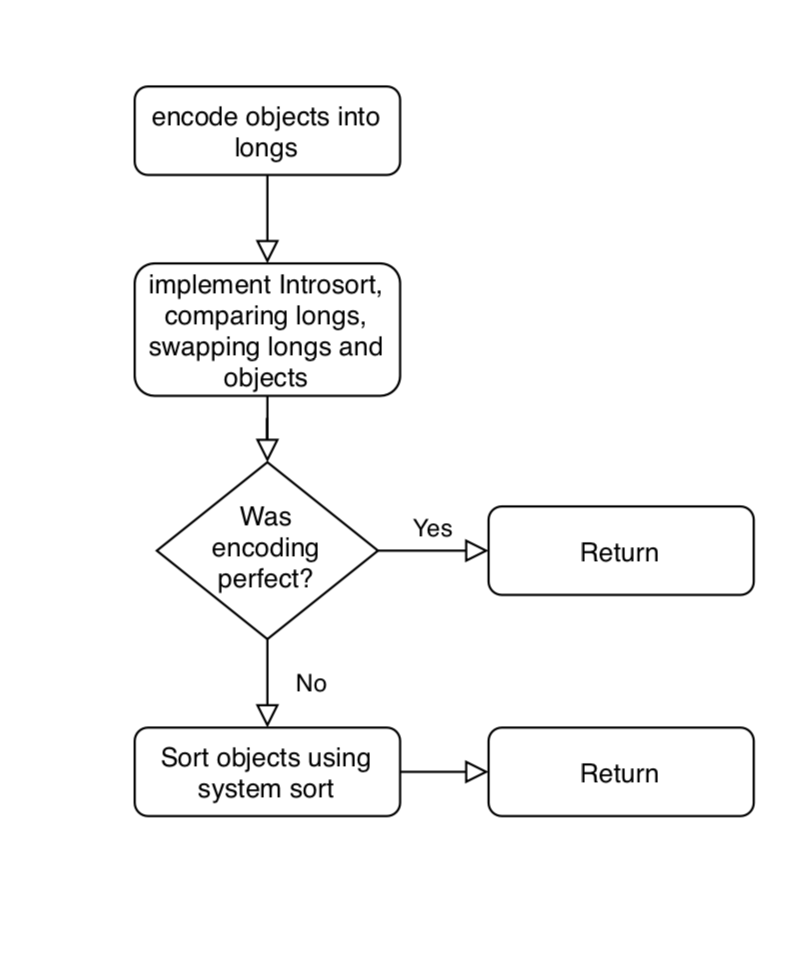
\includegraphics[trim=62 74 22 38, clip, width=0.39\linewidth]{HuskySortFlow.png}
\end{figure}
The strategy of HuskySort (see Flow ~\ref{Fig:HS}) is as follows,
assuming the dataset is presented as an array $xs$ of type $X$:


\begin{steps}
\item  
\renewcommand{\labelenumi}{\alph{enumi}}
    \begin{enumerate}
    \item Create a $long[]$ array (\emph{longs}) of the same size as $xs$;
    \item for each element $x$ of $xs$, set the corresponding element of \emph{longs} to $x.huskyCode()$.
    \end{enumerate}
\item {}Sort array \emph{longs} using quicksort (in practice, we have found that Introsort\cite{doi:10.1002} works well)
in such a way that when elements $i, j$ of \emph{longs} are exchanged, then elements $i, j$ of $xs$ are also exchanged;
\item {}Finally, when quicksort is finished and, if necessary,
we run Timsort on the array $xs$ to ensure that its elements are truly in order.
\end{steps}

For a worked example of a husky coding, see Algorithm ~\ref{alg:permitcoder}

\subsection{RadixHuskySort.}
\label{sec:radix}

Step 2 sorts the husky codes using Introsort, an $\textbf{O}(N log N)$ algorithm,
but the codes themselves are fixed-width 64-bit values,
and radix sort can sort $k$-bit keys in $\textbf{O}(N \cdot \frac{k}{b})$ time using $b$-bit digits —
linear in $N$ for any fixed digit width $b$.
Given that HuskySort's entire premise is to move work from the linearithmic phase to the linear phase,
this raises a natural question we had not previously addressed:
could step 2 itself be made linear? This section describes RadixHuskySort, which we built to answer it (Algorithm ~\ref{alg:the_alg5}).

Radix sort's linear-time advantage rests on a further assumption beyond fixed key width:
that a digit can be turned into an array index in $\textbf{O}(1)$ time,
so that counting and scattering never need to compare two digits directly.
A $b$-bit digit of a husky code satisfies this trivially —
it is extracted by a single shift and mask, and used directly as an index into a $2^b$-bucket counting array.
The original \textit{Comparable} type generally does not:
without first reducing it to such a code, radix sort applied directly to a \textit{String},
a \textit{Tuple}, or a case class would need some other way to decide which of $2^b$ buckets a given key belongs to,
and whenever the natural notion of a "digit" for such a type is not already a small, dense integer,
that decision falls back to \textit{equals} (and, for a hash-based bucket structure,
\textit{hashCode}) on the type itself — an $\textbf{O}(\text{size of the value})$ operation, not an $\textbf{O}(1)$ one.
Husky encoding is what removes this cost from every one of RadixHuskySort's $\frac{64}{b}$ digit passes,
not merely from the final comparison:
once the one-time $\textbf{O}(N)$ encoding step has run,
\textit{equals} and \textit{hashCode} on the original type are not called again until the optional cleanup pass.

A naive adaptation — swapping the object reference alongside each long at every exchange within every digit pass,
exactly as step 2's Introsort swaps at every partition exchange —
would incur $\textbf{O}(N)$ reference movements per digit pass, or $\textbf{O}(N \cdot \frac{64}{b})$ movements in total.
Since $\frac{64}{b}$ is typically much smaller than $log N$ at the sizes we tested,
this would still usually beat Introsort's swap cost,
but it needlessly reintroduces exactly the kind of payload-movement overhead this whole design exists to avoid,
and least-significant-digit (LSD) radix sort's per-pass counting-sort structure makes a better option available.

Instead, RadixHuskySort's step 2 carries only an $\textit{int[]}$ index array through the LSD digit passes,
alongside the (unmodified) long array;
each pass is a stable counting sort keyed on one $b$-bit digit of the (already-computed) husky code,
reordering the index array rather than the codes or the objects themselves.
Once all $\frac{64}{b}$ passes are complete, the index array holds the sorting permutation,
and a single $\textbf{O}(N)$ pass builds the final object array by reading $\textit{xs[index[i]]}$ for each $i$.
This confines all object-reference movement to one pass total, rather than one pass per digit.

Because LSD radix sort's per-digit counting sort treats keys as unsigned,
and husky codes are signed 64-bit values whenever the underlying domain can be negative (e.g., \textit{Integer},
\textit{Long}, or dates before a chosen epoch), each code is first transformed by $\textit{code} \oplus \textit{Long.MIN\_VALUE}$ —
flipping only the sign bit — before the digit passes,
which places negative codes before non-negative ones under unsigned digit comparison without disturbing relative order within either group;
the same transform is idempotent to reverse, so no separate un-flip step is needed once the permutation is built from the transformed codes.
Whether a given \textit{HuskyCoder} can actually produce negative codes is checked rather than assumed,
since several codings (e.g., Unicode strings) never do.

The digit width $b$ is a tunable parameter, trading off the number of passes ($\frac{64}{b}$)
against the size of the per-pass counting array ($2^b$ buckets, which must fit comfortably in cache for each pass to stay fast);
\S~\ref{sec:radix-results} reports how this trade-off plays out empirically across data types and array sizes.
Step 3 (the cleanup pass, run only if the coding is not provably \textit{perfect})
is unchanged regardless of which algorithm sorts the codes in step 2 —
radix sort is a drop-in replacement for that one step, not a change to the overall three-step strategy.

This parameterization also addresses a related limitation:
assuming 64-bit words throughout may not be appropriate for comparison on different key sizes.
Quicksort's asymptotic behaviour does not depend on key width at all —
an $\textbf{O}(N \log N)$ comparison sort costs the same whether the keys being compared are 32 bits or 128 bits wide,
since only the (fixed-cost) comparison itself touches the key's actual bits.
Radix sort, by contrast, makes the key width an explicit, first-class parameter:
a $k$-bit key simply takes $\frac{k}{b}$ passes instead of $\frac{64}{b}$, with no change to the algorithm itself.
So while nothing about the discussion above depends on 64-bit words specifically,
the RadixHuskySort generalizes to other key widths more directly than a comparison-based sort does —
if a future encoding needed, say, 128 bits to capture more of an object's structure,
the same radix sort would apply unchanged, merely with twice as many passes.

Radix sort applied to strings specifically has its own substantial, and older, literature,
distinct from the general fixed-width-key radix sort described above.
Three-way radix quicksort (also called multikey quicksort) and MSD (most-significant-digit)
radix sort for strings were both popularized by Bentley and Sedgewick's classic treatment\cite{314161.314321},
and burstsort\cite{1064546.1180622} improves cache behaviour further by building a small trie to bucket strings before sorting.
These string-specialized algorithms sort variable-length strings directly, character by character, without a separate fixed-width encoding step.
RadixHuskySort's contribution is different in kind, not degree:
it is not a string-sorting algorithm, but a general mechanism applicable to any \textit{Comparable} type
with a 64-bit husky encoding (strings among them),
at the cost of the encoding's own fixed capture window (\S~\ref{sec:pcrit} above)
and a fallback cleanup pass whenever that encoding is imperfect.

That framing carries a consequence which Table ~\ref{tab:RadixImprovements} bears out,
and which we state rather than leave to be noticed:
the string rows of that table are its most variable by a wide margin.
They span from 3.4x down to 1.6x, nearly the whole of its range below dates,
where every other row falls between 2.1x and 3.6x.
Three factors account for the spread, and they compose.
The advantage grows with the cost of the type's native comparison, since that is what the encoding replaces;
it grows with the perfection of the encoding, since an imperfect one is paid for by the cleanup pass;
and it shrinks in the presence of algorithms specialised to the type.
Dates are the favourable extreme on all three counts --- a provably perfect coding, no cleanup pass at all,
and no specialised competitor --- and yield the largest margin in the table at 5.9x.
The string rows show those same three factors varying \emph{within} a single data type,
which is the more instructive demonstration.
Chinese words are favourable on the first two counts --- an expensive Unicode comparison,
captured well enough by the encoding --- and sit fourth of eleven, above all but three of the non-string rows.
Chinese personal names are unfavourable on the second: the comparison is more expensive still,
a table lookup per character, but the pinyin coding captures far less of the key than the Unicode
coding does, so ties are common and the cleanup pass does real work rather than none
(\S~\ref{sec:chinese-coders} accounts for the difference).
The more expensive comparison is paired with the weaker encoding, and this is the weakest result we report.
English words are unremarkable on the first two counts and distinctive on the third,
being the one case in this paper with a mature specialised literature ranged against it.

Strings are unfavourable on the third count in a way no other type in this paper is.
Half a century of specialised string sorting exists,
and a general mechanism should not be expected to beat it on its own ground.
We compared RadixHuskySort against both of the classic string sorts named above,
under JMH, on English and Chinese text, in code-point order so that every sort compared
performs the same task.
Both baselines are our own implementations,
each tuned so that its fallback below the partitioning cutoff allocates nothing
and compares from the depth the partitioning has already established.
Against three-way radix quicksort RadixHuskySort is faster at every size tested,
by 1.3--2.4x on English words and 3.1--4.0x on Chinese words,
with non-overlapping 99.9\% confidence intervals throughout.
Against MSD radix sort the result goes the other way at scale, though not by much:
on English text the two are indistinguishable at $N=32{,}000$,
and MSD is faster by 1.20x at $N=200{,}000$ and by 1.06x at $N=1{,}000{,}000$.
The advantage at $N=200{,}000$ is the robust one.
At $N=1{,}000{,}000$ three runs on the machine of record give 1.00x, 1.05x and 1.06x,
so at the largest size we measure the two algorithms are level to within the spread between runs,
and the direction should be read from the middle size rather than the largest.
We give this result because it locates the boundary rather than obscuring it.
MSD earns it on a corpus that suits it and within limits that are its own:
our implementation indexes an alphabet of 256 characters beyond ASCII,
which English text fits and neither Chinese corpus does,
and it offers no pinyin ordering,
so there is no MSD row for either Chinese corpus.
RadixHuskySort reaches every corpus in this paper through one encoding,
with no per-alphabet provision and no per-type implementation.
That is the claim being made, and the English result bounds it without contradicting it.
A direct empirical comparison against burstsort remains future work;
it is a trie-based, cache-conscious algorithm designed to beat both baselines used here on exactly this workload,
and we have not implemented it.

Code-point order is not a meaningful comparison for Chinese personal names specifically —
it is simply the wrong order for that use case, not merely a different one.
Leaving the word corpus in that order is deliberate: a directory of people has one conventional
ordering and it is by pinyin, where a word list has several --- by radical, stroke count, pinyin or
frequency, according to purpose --- so no single ordering is the right one to hold it to,
and code-point order keeps that row comparable with the English one.
A fair comparison for the names requires a pinyin-aware MultikeyQuicksort.
We extended it with the same syllable-then-tone character key the pinyin encoding of \S~\ref{sec:radix} already uses,
restricted the comparison to the three pinyin-aware sorters, and re-ran it.
RHSort is faster than the repaired multikey quicksort by 1.57x, 1.83x and 2.09x at $N = 32{,}000$,
$200{,}000$ and $1{,}000{,}000$, and QuickHuskySort by 1.33x, 1.49x and 1.27x.
Two independent runs on the machine of record agree to within two hundredths of those multipliers.
Note that the RHSort margin grows with $N$ while QuickHuskySort's does not:
the linear second phase keeps paying as the array grows where a linearithmic one cannot,
which is the same pattern the natural-order corpora show and the clearest form in which this corpus
shows it.

\begin{algorithm2e}
\KwIn{\it{xs} as an array of object X which extends Comparable<X>}
\KwIn{\it{b} as the number of bits per digit}
 coding = huskyCoder.huskyEncode(xs)\;
 longs = coding.longs\;
 index = radixSortIndices(longs, b)\;
 ys = permute(xs, index)\;
 \If{coding.perfect}{return ys\;}
 Arrays.sort(ys)\;
 \caption{RadixHuskySort.sort}
 \label{alg:the_alg5}
\end{algorithm2e}

\begin{algorithm2e}
\KwIn{\it{longs} as an array of long}
\KwIn{\it{b} as the number of bits per digit}
\KwOut{\it{index}, a permutation of $0, \ldots, \textit{longs.length} - 1$ such that
  \textit{longs[index[$\cdot$]]} is sorted}
 biased[i] = longs[i] {\bf XOR} Long.MIN\_VALUE, for each i\;
 index = [0, 1, \ldots, longs.length - 1]\;
 \For{digit = 0 \KwTo (64 / b) - 1}{
 index = stableCountingSortPass(biased, index, digit, b)\;
 }
 \caption{radixSortIndices (LSD, deferred permutation)}
 \label{alg:the_alg6}
\end{algorithm2e}

\subsection{Discussion of Husky Encoding.}

Step 1b requires the definition of a 64-bit hash function (huskyCode) whose properties are as follows:
(refer to Algorithm ~\ref{alg:the_alg2})
\begin{itemize}
                        \item {}If $x = y$, then $x.huskyCode() = y.huskyCode()$;
                        \item {}If $x > y$, then: 
                            \begin{itemize}
                            \item{} either $x.huskyCode() <= y.huskyCode()$ (with probability $p$)
                            \item{} or $x.huskyCode() > y.huskyCode()$ (with probability $1-p$);
                            
                            \end{itemize}
                        
                        \end{itemize}


We interpret this rule as follows:
if $x$ and $y$ are the same ($x.equals(y)$ in Java), their huskyCode should be the same.
If $x > y$, we normally expect that $x.huskyCode() > y.huskyCode()$, i.e., the sort on the husky-coded longs will not invert $x$ and $y$.
However, when $x > y$ while $x.huskyCode() < y.huskyCode()$, then an inversion will be introduced.
And, when $x > y$ and $x.huskyCode() = y.huskyCode()$, then an inversion \emph{may} be introduced because quick-sort is not stable.\cite{6115063}

For a successful encoding, the value of $p$, the probability of a potential inversion, should be less than some critical probability, $p_{crit}$.
Leaving a more detailed discussion of $p_{crit}$ until later, we note that, for some domains of $X$, we can definitely assert that $p = 0$.
We refer to this as a “perfect” encoding.
In such a case, we can skip step 3 of the algorithm because, when $p = 0$, there will be no inversions remaining after quick-sorting according to the huskyCodes.
An example of such a domain is date-time values with a resolution of one nano-second over a period of 128 years.
For strings of English case-independent letters (no punctuation or numbers), i.e., 5-bit ASCII, words of 12 (or fewer) characters in length can also be coded uniquely.
For case-dependent strings (6-bit ASCII), we can encode perfectly if the lengths are all 10 characters or less.
In step 3, it might be acceptable to use insertion sort instead of Timsort.
In any event, assuming that the huskyCode is as accurate as required, then there will be very few inversions (elements out of place) remaining after the quicksort phase.
This implies that the second sort can be performed in very close to linear time.
The results have been very satisfactory.
For example, taking an array of 1,000,000 English words drawn randomly from a corpus of 275,333\cite{GOLDHAHN12.327},
QuickHuskySort sorts in 698 ms against the system sort's 1,121 ms, a factor of 1.61
(for the full data, please refer to table ~\ref{tab:HS_BM}).






\subsection{Discussion of \texorpdfstring{$p_{crit}$}{p\_crit}.}
\label{sec:pcrit}
When $p > 0$, there is a finite probability of any pair of elements remaining inverted after the first sorting pass.
For an array of N randomly ordered elements, the average number of inversions before sorting is $X = N (N -1 ) / 4$.
The number of inversions remaining after the first pass is simply $p X$.
And, for Timsort or insertion sort, the time to re-sort the array will be $t = k (N + p X)$ where $k$ is some system-dependent constant.
The total time to sort the array is made up of these three time-consuming steps where $k_1, k_2, k_3$ are system- and algorithm-dependent constants:

\begin{steps}
 \item{} $T_1$ is the time to encode the elements:
\[T_1 = k_1 N\]
\item{}  $T_2$ is the (average) time to quick-sort the huskyCode array while also swapping the element array itself:
\[T_2 = 2 k_2 N ln N\]
\item{}  $T_3$  is the time to Timsort the element array (only required if $p>0$):
 \[T_3 = k_3 (N + p X)\]
\end{steps}
Provided that the total time $T = T_1 + T_2 + T_3$ is less than the time required to use Timsort on the original element array, we have a win.
This same three-step decomposition ($T_1$/$T_2$/$T_3$, i.e., encode/sort/cleanup) is revisited in \S~\ref{sec:analysis}
in more concrete terms —
counting array accesses directly rather than folding everything into abstract system-dependent constants $k_1, k_2, k_3$ —
and extended there to cover RadixHuskySort (\S~\ref{sec:radix}) as a fourth alternative for the $T_2$ step.
The actual values of $p_{crit}$ are very much dependent on the machine running the sort.
We have not calculated a typical value for $p_{crit}$ but, even for the worst-case:
Chinese characters using UTF8 encoding, we still find very significant gains, reported later in Table ~\ref{tab:HS_BM}.

Of the three terms, $T_3$ can be isolated experimentally.
Two benchmarks over the same two hundred thousand municipal records (\S~\ref{sec:radix-results})
differ only in which coder they are given.
Both compute identical codes; one coder declares itself perfect, so the sort skips step 3,
while the other leaves that declaration at its default and the pass runs.
The encoding for these records is perfect, so the pass that runs has provably nothing to correct.

Its cost is predictable in advance.
Timsort over a fully ascending array detects a single run and stops,
performing $N-1$ comparisons and no moves,
so $T_3$ at $p = 0$ is exactly $N-1$ invocations of the element's own comparator ---
here assessor's block, then lot, then filing date,
which is precisely the comparison the husky encoding was introduced to avoid.
The cleanup pass reintroduces one full composite comparison per element,
having just removed it from all $\textbf{O}(N \log N)$ of them.

That comparison costs 16.1\,ns at $N = 32{,}000$, 60.3\,ns at $N = 100{,}000$ and 74.2\,ns at
$N = 198{,}900$ --- 7.3\%, 17.2\% and 17.3\% of the running time of the sort that contains it ---
with non-overlapping 99.9\% confidence intervals throughout.
Three further runs, one of them on different hardware, agree on the shape at different levels;
across all four the pass costs between a sixteenth and a quarter of the total,
and between a sixth and a quarter at the two larger sizes.
The percentages are the less stable figures, being ratios of two quantities that both move.
The shape is a threshold rather than a trend --- a rise by a factor of roughly three to four between the first two sizes,
then a levelling off --- and it falls where the records stop fitting in cache.
That last reading is inference, but the magnitudes support it:
the system sort compares these same records some 3.5 million times in 151\,ms, or 43\,ns each,
so the cleanup pass at 74\,ns costs nearly twice as much per comparison using the same comparator.
Step 2 permutes references without moving the records,
so a scan sequential in the array is close to random in the heap.

Whether this share must shrink as $N$ grows --- the pass being linear where the sort containing it is
linearithmic --- is a fair question, and \S~\ref{sec:cleanup-scaling} answers it.

Two conclusions follow.
First, $k_3$ is not a constant: it varies more than fourfold across three sizes on one machine,
so no single $p_{crit}$ can be quoted even for one type on one machine.
Second, an encoding which can be declared perfect avoids a cost of up to a quarter of total running
time, where one which cannot must repay it before correcting a single genuine inversion.

\subsection{Why husky coding works.}
\label{sec:why-husky}

The rationale is set out in full by Hillyard et al.\cite{huskysort2020}; we restate only what the rest of
this paper depends on.
A 64-bit word holds enough of most keys to place elements close to their final order, and comparing two
longs costs far less than following two object references and running a type-specific
\textit{compareTo} --- so the encoding trades one $\textbf{O}(N)$ pass for cheaper comparisons throughout
the $\textbf{O}(N \log N)$ one.
The code need not be perfect, only good: whatever inversions it leaves are the cleanup pass's problem, and
\S~\ref{sec:pcrit} measures what they cost.

Perfection has a precise limit for strings.
Packing four 16-bit characters fills the word (Table ~\ref{tab:EncodingConstants} gives the constants for
both string codings), but the packed result is then shifted right by one bit, because any string whose
first character is \texttt{0x8000} or above --- common among CJK characters --- would otherwise set the
sign bit and encode as a negative \textit{long}, corrupting numeric comparison.
The shift costs the least significant bit of a true fourth character; for three characters or fewer that
bit is padding, which is why the Unicode coding is declared \textit{perfect} up to three characters and
not four.

Whether a coding was in fact perfect is known before the cleanup pass runs: a constant-time lookup for
non-sequence types, and for strings a scan that stops at the first string too long to encode perfectly.
Where it was perfect, no inversions remain and the pass is skipped altogether.


\begin{algorithm2e}
\KwIn{\it{xs} as an array of object X}
\KwOut{A new \it{Coding} object}
 result = new long[xs.length]\;
 \For{i = 0 to xs.length}{
 result[i] = huskyEncode(xs[i])\;
 }
 return new Coding(result, perfect())\;
 \caption{huskyEncode}
 \label{alg:the_alg2}
\end{algorithm2e}


\begin{algorithm2e}
\KwIn{\it{permit}, with fields \it{block}, \it{lot}, \it{filedDate}\;}
\KwOut{a 60-bit code, order-preserving for \it{permit.compareTo}}
 \tcp{fields most-significant first, in compareTo order}
 r = encodeString(block, 5, 5, BLOCK\_ALPHABET)\;
 r = r $\ll$ 24 $|$ encodeString(lot, 4, 6, LOT\_ALPHABET)\;
 \Return r $\ll$ 11 $|$ daysSinceEpoch(filedDate)\;
 \BlankLine
 \tcp{codeOf(x, alphabet), used by encodeString for each symbol}
 \eIf{alphabet contains x}{
   \Return 1 + index of x\tcp*{0 is left for padding}
 }{
   \Return count of symbols $<$ x\tcp*{weaken, never invert}
 }
 \caption{A composite husky coder: \textit{PermitCoder}. \textit{encodeString} packs \textit{width}
   symbols of \textit{bits} each, right-padding with zero.}
 \label{alg:permitcoder}
\end{algorithm2e}

\section{Implementation.}

%% ANONYMISATION: the real URL names its owner, so it is guarded with the author block. See
%% "0i. The repository link" in Paper edits pending.md -- the Anonymous GitHub mirror is task 2
%% on Sai Vineeth's list; when its URL exists, substitute it for the placeholder below and the
%% review copy can cite the code directly.
\ifanonymous
  The implementation is available in an anonymised repository, linked from the submission site.
\else
  The implementation is available at \url{https://github.com/rchillyard/HuskySort}.
\fi

\subsection{System Environment.}

Three machines appear in this paper, and \S~\ref{sec:environments} specifies all three.
Machine A ran the JDK 1.8.0\_152 comparison-sort benchmarks of \S~\ref{sec:analysis},
the choice of cleanup sort among them (\S~\ref{sec:cleanup-choice});
machine B, on different hardware and two JVM generations later, ran the radix-sort and JMH development work.
Machine C is the machine of record: an independently administered cloud instance, confirmed idle before
each run, and the source of every figure quoted in this paper.
It is ARM-based like machine B but differs from it in core design, vendor, core count and operating system.

Reporting all three lets a reader check directly whether the qualitative finding generalizes across
machines and JVM versions rather than being an artifact of one environment.
It does: QuickHuskySort, and now RHSort, beat the system sort on all three,
which differ in vendor, instruction set, core design and JVM generation.



\begin{table}
  \caption{String-encoding constants}
  \label{tab:EncodingConstants}
  \begin{tabular}{lll}
    \toprule
    Constant & Unicode & ASCII \\
    \midrule
    Bit width per character & 16 & 7 \\
    Max length (64 / bit width) & 4 & 9 \\
    Mask & \texttt{0xFFFF} & \texttt{0x7F} \\
    \bottomrule
  \end{tabular}
\end{table}

\section{Test Case and Analysis.}

\subsection{Data Source.}
\label{sec:data-source}
The sources for the Strings (English and  Chinese) are retrieved from Leipzig Corpora Collection\cite{GOLDHAHN12.327}.
Chinese personal names, used for the pinyin-order comparisons of \S~\ref{sec:radix-results}, are a separate corpus\cite{wainshine2020chinesenames}.
Every other dataset in this paper is generated: pseudo-random numbers, dates and tuples.
The building-permit records of \S~\ref{sec:radix-results} are not.
They are 198,900 permits filed between January 2013 and February 2018, taken from San Francisco's published
record\cite{sf-building-permits} and ordered by a composite key of assessor's block, lot and filing
date; they are included because their distribution is the city's rather than ours.
Only those three columns are retained, and the data is used under the Open Data Commons Database
Contents License.

In each case, we take data from the appropriate \emph{sentences.txt} file and break it up into strings as shown in Listing~\ref{lst:DS}.


\begin{lstlisting}[caption={Data Source},label={lst:DS},language=Java]
private static String[] getLeipzigWordsFromResource(final String resource) {
    return getWords(resource, HuskySortBenchmark::getLeipzigWords);
}
private static List<String> getLeipzigWords(final String line) {
    return HuskySortBenchmarkHelper.splitLineIntoStrings(line, REGEX_LEIPZIG, REGEX_STRINGSPLITTER);
}
final static Pattern REGEX_LEIPZIG = Pattern.compile("[~\\t]*\\t(([\\s\\p{Punct}\\uFF0C]*\\p{L}+)*)");
public static final Pattern REGEX_STRINGSPLITTER = Pattern.compile("[\\s\\p{Punct}\\uFF0C]");


static List<String> splitLineIntoStrings(final String line, final Pattern lineMatcher, final Pattern stringsplitter) {
    final Matcher matcher = lineMatcher.matcher(line);
    if (matcher.find()) return Arrays.asList(stringsplitter.split(matcher.group(1)));
    else return new ArrayList<>();
}

static String[] getWords(final String resource, final Function<String, List<String>> stringListFunction) {
    try {
        File file = new File(getPathname(resource, DutchHuskySort.class));
        return getWordArray(file, stringListFunction, 2);
    } catch (FileNotFoundException e) {
        logger.warn("Cannot find resource: "+resource, e);
        return new String[0];
    }
}
    } catch (final Exception e) {
        throw new RuntimeException(e);
    }
}


\end{lstlisting}

\subsection{Analysis.}
\label{sec:analysis}
Let’s try to do an analysis of QuickHuskySort's performance.
This expands on the $T_1$/$T_2$/$T_3$ decomposition introduced in \S~\ref{sec:pcrit} above,
replacing its abstract time constants with concrete array-access counts,
and extending it to cover RHSort (\S~\ref{sec:radix}) as an alternative to quicksort for the $T_2$ step.
The first thing to note is that, like merge sort, QuickHuskySort requires $\textbf{O}(N)$ extra space.
This is because, in addition to the array of object references, we must have an equal-length array of longs (the huskyCode values).

Secondly, QuickHuskySort is not stable unless using the merge sort variation.
The derivation of the two comparison figures is a counting argument rather than a measurement, and it
rests on one coefficient we estimated rather than measured; it is set out in \S~\ref{sec:qhs-analysis}.

Encoding's cost has not simply been assumed:
we timed the encoding phase in isolation,
separately from the sort that follows it, to confirm it directly.
At $N = 1{,}000{,}000$, encoding takes 67.7ms for English words (9.7\% of QuickHuskySort's 697.9ms total,
24.8\% of RHSort's 272.7ms) and 211.1ms for Chinese names encoded via pinyin (16.9\% of QuickHuskySort's
1252.7ms, 27.8\% of RHSort's 760.9ms) — confirming that encoding cost, while real and non-negligible,
especially for the more elaborate pinyin encoding, remains a minority of total time in every case measured,
consistent with the linear-and-subordinate role it is assumed to play above.
Encoding's share of the total is larger for RadixHuskySort than for QuickHuskySort in both cases,
simply because RHSort's own contribution to the total is smaller —
as the sort phase gets cheaper,
whatever cost remains in the encoding phase necessarily becomes a proportionally larger slice of what is left,
which suggests encoding cost (particularly for pinyin)
is the more promising target for further optimization now that the sort phase itself is no longer the dominant cost.
The consequence of this is that, as expected,
the linear phase of QuickHuskySort is relatively high for small $N$ but that is soon swamped by the saving of comparisons in the linearithmic phase.
The break-even point is actually a very small value of $N$:
four.
As $N$ increases, we expect the advantage of QuickHuskySort to increase further.
This is generally borne out by the benchmarks.
Please refer to table ~\ref{tab:Comparison}.

The same style of analysis extends naturally to RadixHuskySort (\S~\ref{sec:radix}).
Each of its $\frac{64}{b}$ digit passes touches every element a small constant number of times,
$c$, to bucket it and to record its new position in the (deferred) index array —
with no partitioning or pivot-comparison overhead, and critically, no logarithmic term at all.
Taking $c = 4$ (the same per-exchange cost used for QuickHuskySort's swaps above),
adding the final $\textbf{O}(N)$ pass that applies the resulting permutation to the object array (2 array accesses per element),
and the same encoding cost ($(k+1)N$) and cleanup-pass cost ($(2 + j + 4)pN$,
unaffected by which algorithm sorts the codes in step 2), the total array accesses for RadixHuskySort ($A_r$) come to:
\[A_r = \left(4 \cdot \frac{64}{b} + 2 + k + 1\right) N + (2 + j + 4)pN\]
Using the same illustrative constants as above ($j = 4$, $k = 7$, $p = 0.1$)
and $b = 16$ (four digit passes, near the middle of the digit-width plateau found empirically —
see \S~\ref{sec:radix-results}):
\[A_r = 27 N\]
Table ~\ref{tab:Comparison} extends the earlier comparison with this term.
At $N = 1{,}000{,}000$, $A_r \approx 27{,}000{,}000$ against $A_h \approx 101{,}000{,}000$ and $A_m \approx 161{,}000{,}000$ —
a predicted advantage of roughly 3.7x over QuickHuskySort,
consistent with the 2-4x speedups actually measured (\S~\ref{sec:radix-results}).
The model does predict one caveat:
equating $A_r$ and $A_h$ gives a theoretical break-even around $N \approx 17$,
somewhat higher than QuickHuskySort's own break-even against merge sort ($N = 4$,
above) — because RHSort's per-pass cost has no logarithmic term to shrink relative to at very small $N$.
This crossover is far below every array size actually tested, so it has no practical effect on the results reported here,
but it is worth stating rather than leaving the model looking like radix wins unconditionally at every $N$.
 \begin{table*}
  \caption{Theoretical comparisons (array accesses, dimensionless counts)}
  \label{tab:Comparison}
  \begin{tabular}{rrrrr}
    \toprule
    N  &  N ln N & merge sort & QuickHuskySort & RHSort \\
    \midrule
     4 & 6 & 72 & 72 & 108 \\
     1,000 & 6,908 & 81,439 & 55,075 & 27,000 \\
     1,000,000 & 13,815,511 & 160,878,371 & 101,149,455 & 27,000,000 \\
     1,000,000,000 & 20,723,265,837 & 240,317,557,125 & 147,224,183,132 & 27,000,000,000 \\

    \bottomrule
  \end{tabular}
\end{table*}

Since the final pass of HuskySort will be cleaning up a relatively small number of inversions, does it
matter whether we use insertion sort or Timsort?
Below about 50,000 Strings it makes barely any difference, and insertion sort is sometimes faster;
beyond that Timsort wins out, by a factor of four and a half at $N = 4{,}000{,}000$.
That measurement, and the choice it settles, are in \S~\ref{sec:cleanup-choice}.


\section{Results and Observations.}
\subsection{Benchmarks.}

Table ~\ref{tab:HS_BM} reports absolute sort times for every data type and corpus.
The two radix columns bracket the digit-width plateau of \S~\ref{sec:radix-results}.
Dual-pivot quicksort and a from-scratch quicksort were measured too; they bear on QuickHuskySort
rather than on RHSort, so they are in \S~\ref{sec:comparison-baselines}.

\begin{table*}
  \caption{Sort times by data type (JMH, ms, mean $\pm$ 99.9\% CI). Numeric types at $N=500{,}000$.
    For Chinese names the system-sort column is a system sort performing the same pinyin ordering;
    code-point order is a different and much cheaper task (\S~\ref{sec:radix-results}).}
  \label{tab:HS_BM}
  \begin{tabular}{llllll}
    \toprule
    Data type & N & System sort & QuickHuskySort & RHSort/8 & RHSort/16 \\
    \midrule
    Integer & 500,000 & 121.2$\pm$0.6 & 89.7$\pm$3.5 & 31.2$\pm$0.5 & 25.2$\pm$0.2 \\
    Double & 500,000 & 141.7$\pm$1.3 & 97.8$\pm$3.6 & 34.0$\pm$0.5 & 31.0$\pm$0.3 \\
    Long & 500,000 & 135.8$\pm$1.2 & 97.7$\pm$1.0 & 30.2$\pm$0.2 & 28.6$\pm$0.3 \\
    BigInteger & 500,000 & 208.4$\pm$1.7 & 152.3$\pm$1.7 & 56.9$\pm$0.3 & 54.1$\pm$0.2 \\
    BigDecimal & 500,000 & 262.2$\pm$1.6 & 144.1$\pm$2.1 & 54.1$\pm$0.3 & 52.5$\pm$0.3 \\
    English words & 32,000 & 13.69$\pm$0.19 & 9.72$\pm$0.12 & 4.63$\pm$0.16 & 4.18$\pm$0.16 \\
    & 200,000 & 141.39$\pm$2.59 & 94.74$\pm$2.44 & 55.01$\pm$2.20 & 50.27$\pm$2.51 \\
    & 1,000,000 & 1120.87$\pm$14.43 & 697.88$\pm$16.15 & 355.26$\pm$24.71 & 272.74$\pm$6.46 \\
    Chinese words & 32,000 & 9.78$\pm$0.08 & 5.00$\pm$0.04 & 2.10$\pm$0.03 & 1.89$\pm$0.02 \\
    (code-point order) & 200,000 & 71.34$\pm$0.63 & 30.90$\pm$0.13 & 13.49$\pm$0.15 & 10.85$\pm$0.10 \\
    & 1,000,000 & 447.12$\pm$2.28 & 219.80$\pm$1.99 & 83.25$\pm$2.31 & 65.46$\pm$1.47 \\
    Chinese names & 32,000 & 69.1$\pm$1.4 & 26.6$\pm$0.3 & 24.1$\pm$0.2 & 23.1$\pm$0.3 \\
    (pinyin order) & 200,000 & 526.2$\pm$9.5 & 187.2$\pm$1.0 & 157.0$\pm$1.3 & 154.9$\pm$1.2 \\
    & 1,000,000 & 3112.9$\pm$68.0 & 1252.7$\pm$6.4 & 775.7$\pm$4.2 & 767.2$\pm$14.0 \\
    Tuples & 20,000 & 3.72$\pm$0.01 & 2.79$\pm$0.02 & --- & 1.30$\pm$0.01 \\
    & 100,000 & 23.24$\pm$0.19 & 17.65$\pm$0.16 & --- & 6.82$\pm$0.05 \\
    & 500,000 & 209.53$\pm$7.98 & 142.61$\pm$1.83 & --- & 57.98$\pm$0.76 \\
    \bottomrule
  \end{tabular}
\end{table*}

\subsection{Summary.}
\label{sec:summary}
HuskySort’s target application is the sorting of randomly ordered arrays of objects on the JVM (Java Virtual Machine).
Let’s eliminate the non-use-cases first:
\begin{itemize}
\item {}Partially-ordered arrays:
that’s to say, arrays with only a linear number of inversions as would be the case when adding a relatively small number of records to a large existing index.
For such use cases, Timsort (the Java system sort for objects) would be more suitable.

\item {}Arrays of primitives:
in Java, a clear distinction exists between primitive types (char, byte, short, int, float, long, double) and objects.
Dual-pivot quicksort (the Java system sort for primitives) is already the fastest algorithm for sorting such types.
\end{itemize}
Thus, HuskySort is best for any object array where there’s no expectation of partial ordering.
Typical improvements over Timsort can be read directly off Table ~\ref{tab:HS_BM} above, which gives
absolute times with 99.9\% confidence intervals rather than summary ranges:
1.4--1.8x across the five numeric types at $N=500{,}000$,
1.4--1.6x on English words,
2.0--2.3x on Chinese words,
and 1.3--1.5x on tuples.
Note that the English margin \emph{widens} with array size rather than decaying,
from 1.41x at $N=32{,}000$ to 1.61x at $N=1{,}000{,}000$.

\subsection{Radix Sort Results.}
\label{sec:radix-results}

We benchmarked every data type and corpus covered above using RadixHuskySort (\S~\ref{sec:radix})
in place of Introsort for step 2, using JMH (the Java Microbenchmark Harness, with proper fork isolation and warmup) on JDK 21.

Table ~\ref{tab:RadixImprovements} reports RHSort's advantage over QuickHuskySort as a direct multiplier —
e.g., \textbf{2.9x} means radix took roughly a third as long —
rather than as a percentage, since a percentage figure close to or above 100\% becomes ambiguous about exactly which quantity it is a percentage \emph{of}.

\begin{table*}
  \caption{RHSort's advantage over QuickHuskySort, as a direct multiplier}
  \label{tab:RadixImprovements}
  \begin{tabular}{cll}
    \toprule
    Data Type & N & Advantage over QuickHuskySort \\
    \midrule
    \texttt{Dates} & 20,000 & 5.9x \\
    \texttt{Long} & 500,000 & 3.6x \\
    \texttt{Integer} & 500,000 & 3.6x \\
    \texttt{Strings of Chinese words (code-point order)} & 1,000,000 & 3.4x \\
    \texttt{Double} & 500,000 & 3.2x \\
    \texttt{BigInteger} & 500,000 & 2.8x \\
    \texttt{BigDecimal} & 500,000 & 2.8x \\
    \texttt{Strings of English words} & 1,000,000 & 2.6x \\
    \texttt{Tuples} & 500,000 & 2.5x \\
    \texttt{Building permits (composite key)} & 198,900 & 2.1x \\
    \texttt{Strings of Chinese names (pinyin order)} & 1,000,000 & 1.6x \\
    \bottomrule
  \end{tabular}
\end{table*}

This is worth confronting directly, since a reader might reasonably ask whether either advantage erodes
as $N$ grows: a constant-factor saving on a linearithmic sort could be swamped at scale.
Neither does.
QuickHuskySort's margin over the system sort on English text \emph{widens} with size,
from 1.41x at $N=32{,}000$ to 1.49x and then 1.61x (Table ~\ref{tab:HS_BM}),
and holds roughly constant on both Chinese corpora.
Radix sort's advantage over QuickHuskySort likewise does not shrink with $N$:
at every size and data type in Table ~\ref{tab:RadixImprovements}, the margin is 1.5x or greater,
consistent with the theoretical model of \S~\ref{sec:radix} predicting no logarithmic term at all,
so there is no analogous reason to expect the advantage to erode as $N$ grows further.
The spread across that table is itself informative, and follows the three factors of \S~\ref{sec:radix}.
Chinese names sorted by pinyin order are the smallest margin measured (1.6x),
because both QuickHuskySort and RadixHuskySort must pay the same cleanup pass for a coding
that two or three characters of recurring syllables leave badly imperfect.
Dates show the largest margin (5.9x) because that coding is provably perfect and never needs a cleanup pass at all,
letting RHSort's linear-time advantage show through with nothing else in the way.
The two lie at opposite ends of the same axis: what separates them is not the data type but the perfection of the encoding.

The building permits row is the only one in that table not measured on data we generated:
198,900 real municipal records ordered by a composite key of three fields (\S~\ref{sec:data-source}).
At 2.1x it is tenth of eleven, which is the point worth making about it --- it is not our largest
margin, but it is our largest on data whose distribution we did not choose.
\S~\ref{sec:permits} gives the case study, and \S~\ref{sec:composite-future} what a general
composite encoder would have to provide, that one having been written by hand.

The measurements were reproduced qualitatively on machines A and B of \S~\ref{sec:environments},
which differ from the machine of record and from each other in vendor, instruction set, core design and
JVM generation.
We quote no figures from them, since mixing environments within a comparison would rob it of meaning,
but every ordering reported here holds on all three.

\subsection{Parallel Radix Sort.}
\label{sec:parallel-radix}

Radix sort's digit passes are natural candidates for parallelization (\S~\ref{sec:radix} above).
We implemented and benchmarked a parallel variant:
each pass is split into a configurable number of contiguous chunks, one per worker thread.
Every chunk first computes its own local per-bucket histogram independently, with no synchronization required;
a short sequential step then combines those histograms into an exact starting offset, in the output array,
for every (chunk, bucket) pair — preserving the stability that step 3's cleanup pass, when needed, relies on,
since a chunk's elements always land after all lower-numbered chunks' elements sharing the same bucket;
finally, every chunk scatters its own elements into the output arrays independently,
using only its own precomputed offsets, so no two chunks ever write to the same location.

An initial implementation dispatched the two phases above to a thread pool separately on every pass.
Measurement showed this repeated dispatch itself contributing a real, non-trivial share of the total cost,
particularly at more moderate array sizes.
The overhead was substantially reduced by starting the worker threads once per sort,
rather than once per phase per pass:
each thread runs its own loop over every pass, and the two phases synchronize via reused barriers whose associated actions —
code that runs exactly once per synchronization point, in whichever thread arrives last —
perform the histogram-combine and buffer-swap steps.
Table ~\ref{tab:ParallelRadix} reports the result (\textit{Long[]}, 11-bit digits, milliseconds, mean $\pm$ 99.9\% CI).

\begin{table*}
  \caption{Parallel RHSort:
serial vs. 1, 2, 4, and 8 worker threads}
  \label{tab:ParallelRadix}
  \begin{tabular}{cccccc}
    \toprule
    N & Serial & 1 thread & 2 threads & 4 threads & 8 threads \\
    \midrule
    2,000,000 & 172.0$\pm$5.7 & 165.2$\pm$2.2 & 140.3$\pm$2.0 & 118.5$\pm$2.4 & 109.3$\pm$1.8 \\
    10,000,000 & 935.2$\pm$36.9 & 884.5$\pm$21.6 & 731.6$\pm$19.9 & 687.9$\pm$22.1 & 645.3$\pm$20.9 \\
    \bottomrule
  \end{tabular}
\end{table*}

Isolating parallelism itself, that's to say comparing 1 thread against 4, both paying identical thread-coordination overhead,
gives a statistically resolved speedup at both sizes: 1.39x at $N=2{,}000{,}000$ and 1.29x at $N=10{,}000{,}000$,
with non-overlapping confidence intervals in both cases.
Against the serial implementation the improvement is resolved at both sizes too,
172.0ms to 118.5ms at $N=2{,}000{,}000$ and 935.2ms to 687.9ms at $N=10{,}000{,}000$.
Unlike on the eight-core machine of an earlier draft, scaling does not stop at four threads:
on sixteen uniform cores, eight threads beats four at both sizes with intervals that do not overlap,
reaching 1.51x and 1.37x over a single thread.

That is still well short of linear, and the shortfall is the more interesting number:
an eightfold increase in threads buys between 1.4x and 1.5x,
on hardware with no performance/efficiency asymmetry to account for it.
Two explanations fit, and we cannot separate them without hardware counters.
Each digit pass scatters across the whole array, so the sort may simply be limited by memory throughput,
which extra cores do not supply; and each pass's histogram-combine step is sequential,
running once per synchronization point whatever the thread count,
so it grows as a share of the total as threads are added.
The first would be a property of the machine and the second of the design,
and only the second would survive better hardware.

\subsection{Use-Case Guidance.}
\label{sec:usecase}

\S~\ref{sec:summary} already eliminates two cases outright:
partially-ordered arrays, where Timsort's own adaptivity wins, and arrays of already-cheap-to-compare primitives,
where dual-pivot quicksort is already the fastest option.
For the remaining case — arrays of objects with no expectation of partial ordering —
the decision is governed by the three factors of \S~\ref{sec:radix}
rather than by the size of the array,
and Table ~\ref{tab:Guidance} puts them in the order a practitioner can answer them.
Size enters only once those are settled, and then only near the bottom of the range.

\begin{table*}
  \caption{Which sort to reach for. The situations are ordered by how much they decide, and
    array size settles nothing until all of them are.}
  \label{tab:Guidance}
  \begin{tabular}{p{0.42\textwidth}p{0.24\textwidth}p{0.26\textwidth}}
    \toprule
Your situation & Reach for & Evidence \\
    \midrule
    The ordering is already cheap to evaluate --- primitives, or a single numeric field
      & dual-pivot quicksort & cost of encoding cannot be recouped (\S~\ref{sec:summary}) \\
    The ordering is composite or expensive, \emph{and} the key packs exactly into 64 bits
      & RadixHuskySort; no cleanup pass is required
      & the largest margins we measure: dates 5.9x, building permits 2.1x over QuickHuskySort \\
    The ordering is composite or expensive, but the encoding is imperfect
      & RadixHuskySort, even allowing for the cleanup pass
      & that pass costs a sixth to a quarter past $N=100{,}000$, even with nothing to correct
        (\S~\ref{sec:pcrit}) \\
    A sort specialised to your type already exists
      & use it, if it covers your data
      & on English words a tuned MSD radix sort beats us, though our MSD indexes extended
        ASCII only and cannot sort either Chinese corpus (\S~\ref{sec:radix}) \\
    The data defeats the encoding's capture window --- long shared prefixes, or keys wider than
    the coder can see
      & System sort & every husky variant loses its advantage (\S~\ref{sec:adversarial}) \\
    None of the above settles it, or the keys are strings
      & by array size (\S~\ref{sec:usecase})
      & each sort's fixed setup cost is repaid at a different $N$ \\
    \bottomrule
  \end{tabular}
\end{table*}

Only when all of those are answered does array size matter, and then chiefly at the small end,
where each algorithm's fixed setup cost has not yet been amortized.
For String keys we measured every crossover directly (JMH, English corpus, $N=4$ through $10{,}000$).
System sort is the fastest of the group up to $N=20$, though only narrowly there
(0.462$\mu$s against insertion sort's 0.489$\mu$s).
A plain, binary-search-based insertion sort wins outright from $N=50$ through $N=200$ —
the one regime in this paper where plain insertion sort,
not either HuskySort variant, is the best available choice.
QuickHuskySort takes over between $N=200$ and $N=500$, and remains the best choice up to roughly $N=2{,}000$,
since RadixHuskySort's own fixed setup cost is not yet amortized below that point.
That cost can be read directly off the measurements: RadixHuskySort's time is a near-constant
166$\mu$s floor from $N=4$ to $N=500$, the allocation and initialisation of its counting structures,
which only the linear term begins to dominate past a few thousand elements.
Somewhere between $N=2{,}000$ and $N=10{,}000$ it takes over;
its advantage then grows and holds at every larger size tested (Table~\ref{tab:RadixImprovements}).
Every one of these crossovers shares the same shape:
each successive algorithm carries a larger fixed setup cost that only pays for itself once there is enough work to amortize it against —
the same fixed-vs-variable-cost story \S~\ref{sec:parallel-radix} found one level further down,
where ParallelRHSort's own thread/barrier setup only pays off once there is enough work to divide across threads.
These crossover points were measured only for String keys.
The fixed costs involved are architectural rather than type-specific,
so other key types plausibly show similarly-shaped curves at similar sizes,
though that has not been separately confirmed.

Two further caveats from elsewhere in this paper complete the picture.
If the source data defeats the husky encoding's fixed capture window entirely —
a shared prefix longer than the encoding's own character limit, for instance —
neither QuickHuskySort nor RadixHuskySort helps regardless of $N$ (\S~\ref{sec:adversarial}):
both lose to plain System sort, since the encoding pass becomes pure waste and the mandatory cleanup pass must do all the real work anyway.
And given a large enough workload and spare cores, \textit{ParallelRadixHuskySort}
widens RadixHuskySort's own advantage further still (\S~\ref{sec:parallel-radix}),
provided there is enough total work to amortize its own thread-coordination cost.

\section{Conclusion.}

The original idea behind HuskySort, that's to say QuickHuskySort,
was to shift work from the linearithmic phase of sorting to the linear phase (both the prelude and the postlude)
and effect an overall reduction in array accesses and thus processing time.
\label{sec:conclusion-dp}%
This has been demonstrated such that, when sorting objects rather than primitives,
HuskySort is faster than dual-pivot quicksort wherever the ordering is expensive to evaluate ---
by 1.4x on \textit{BigInteger} and 1.7x on \textit{BigDecimal} (\S~\ref{sec:comparison-baselines}).
On \textit{Integer}, \textit{Double} and \textit{Long}, where a comparison costs almost nothing,
the encoding has nothing to amortise and dual-pivot quicksort is ahead instead, by up to a tenth.
That is the same criterion which governs every other result in this paper,
here separating one group of numeric types from another.
It is faster than Timsort for arrays which are not partially ordered, above a few hundred elements;
below that, Timsort's own tuned handling of small arrays wins instead.
It is especially fast for types whose ordering is composite or expensive to evaluate
and whose keys encode perfectly, where the encoding replaces the whole comparison and no cleanup pass is needed.
Strings are not reliably that case:
they are the one domain with a mature specialised literature of its own (\S~\ref{sec:radix}),
and they are also the most variable, spanning nearly the whole range of our results ---
including the narrowest margin we report, for Chinese personal names in pinyin order.

In the case of RadixHuskySort, the performance improvement is even better for datasets above a few thousand in length.
Of course, in this case, there was no linearithmic phase, so the time savings come, as explained above,
from more bit manipulation and fewer calls to \textit{equals}.

These findings are not an artifact of a single development machine.
The same qualitative pattern held on three environments spanning two CPU vendors and three distinct architectures
(\S~\ref{sec:environments}),
the last a 16-core ARM server instance with no performance/efficiency core split to confound the result.
That same run also settled a question the parallel variant's own results had left open (\S~\ref{sec:parallel-radix}):
its scaling ceiling past a handful of threads is a property of the design itself,
the fixed sequential cost of combining per-thread histograms once per pass,
not an artifact of any one machine's particular mix of core types.

HuskySort's advantage is specific to a particular kind of workload rather than universal, and needs
all three of the following to hold: an array of at least a few hundred elements, growing to a few
thousand before RadixHuskySort's own per-pass setup cost is repaid (\S~\ref{sec:usecase});
no expectation of pre-existing order, which favours Timsort's adaptivity instead (\S~\ref{sec:summary});
and a comparison costing more than a single machine-word check --- strings, arbitrary-precision numbers
and multi-field records, as opposed to \textit{int}, \textit{long} or \textit{double},
where dual-pivot quicksort already wins outright.

%%
%% The acknowledgments section is defined using the "acks" environment
%% (and NOT an unnumbered section). This ensures the proper
%% identification of the section in the article metadata, and the
%% consistent spelling of the heading.
%% Guarded with the author block: naming collaborators identifies the authors as surely as
%% the author block does, so the review copy carries no acknowledgments at all.
\ifanonymous\else
  \section*{Acknowledgments}
  To Darshan Dedhia, Akshay Bhusare, Kartik Kumar for their help with this project.
\fi



%%
%% The next two lines define the bibliography style to be used, and
%% the bibliography file.
\bibliographystyle{siamplain}
\bibliography{sample-base}

%%
%% If your work has an appendix, this is the place to put it.
\appendix
\section{Appendix.}
\subsection{The array-access analysis of QuickHuskySort.}
\label{sec:qhs-analysis}

\S~\ref{sec:analysis} counts array accesses for RHSort and compares the result with QuickHuskySort and
merge sort in Table ~\ref{tab:Comparison}. This section derives the two comparison figures.

It is a counting argument, and one step in it is an estimate rather than a count: the factor of 0.6
below, which stands for the proportion of object-reference swaps whose targets have not already been
fetched into cache. We have not measured it. Everything else here is arithmetic over the operation
counts of the algorithms concerned, and the RHSort figure in \S~\ref{sec:analysis} needs no such
factor --- $4 \cdot 64/b$ digit passes is a count, not an estimate. The comparison should be read as an
order-of-magnitude argument, which is all the paper asks of it; the measurements of
\S~\ref{sec:radix-results} are what carry the result.

How many comparisons and swaps does QuickHuskySort require, on average?
Wild and Nebel's average-case analysis of dual-pivot quicksort\cite{WildNebel12} gives, approximately:
\begin{itemize}
    \item Comparisons: $1.9 N ln N$;
    \item Swaps: $0.6 N ln N$.
\end{itemize}

A comparison reads two array elements, though because one comparand is always the pivot --- already
in hand --- the effective count is closer to one.
Each swap requires 4 array accesses, although again, we will be swapping elements that have already been accessed.
The effective number of (normalized) array accesses is, in total, approximately 4 rather than the expected 3.8 + 2.4.
That is to say, the coefficient of $N ln N$ is approximately 4.
The analysis represented by the table is for dual-pivot quicksort.
\footnote{Note that, since dual-pivot quicksort is not actually implemented in the Java library for Comparable objects,
    we re-implemented the class for objects.}
However, in QuickHuskySort, each swap also must swap the object references.
These will not, in general, have been pre-fetched and so the effective total normalized array accesses ($A$) is approximately:
\[A = 4 + 0.6 * 4 = 6.4\]
Additionally, QuickHuskySort requires $N$ huskyCode constructions.
Each of these requires $k+1$ array accesses where $k$ is proportional to the number of fields contributing to the huskyCode.
For a string,
that will be the number of characters in the string (except that this is limited to a relatively small number according to the encoding).
For ASCII strings, it is nine.
For Unicode strings, it is four.

However, keep in mind that this is linear and, while it can’t be completely ignored,
it doesn't contribute to the overall growth of the complexity.

Once the sort of the codes is complete, we will assume that there are $p N$ remaining inversions,
where $p$ is the probability of an idiogenic (self-inflicted) inversion.
Again, while we should not ignore it completely, it is linear.
The number of array access for the comparisons/swaps to fix these will be $(2 + j + 4) p N$,
where $j$ is the number of fields to be compared to get a result ($j$ is usually smaller than $k$).

So, the total number of array accesses ($A$) for Husky-sorting an array of length $N$ is:
\[A = (6.4 ln N + (2 + j + 4) p + k + 1) N\]
   
Timsort would be hard to analyze in the general case and so we instead analyze merge sort,
which should be approximately the same number of array accesses in the average case.
 
For merge sort, the analysis is much simpler:
the number of comparisons for a randomly ordered array of length $N$ is $N log_2 N$.
Merge sort does not use swaps, \emph{per se}, but instead uses copies.
Assuming that we optimize the extra copying, there will be $N$ copies to get the algorithm started and $N$ per level.
Thus, the number of copies will be $N {log_2 N}$.
Each of these copies requires two array accesses while each comparison requires 2 + j (described above) array accesses.
 
The total number of array accesses ($A$) for merge sort is, therefore:
\[A = (4 + j) N log_2 N + 2 N\]
 
Given that $log_2 N = 1.44 ln N$, and assuming that:

$j = 4$ corresponding to the comparison of two strings that start with the same character but differ in the second character; and

$k = 7$ and $p = 0.1$; then

the totals ($A_m$ for merge sort and $A_h$ for QuickHuskySort) come to:
 \[A_m = 11.5 N ln N + 2 N\]
 \[A_h = 6.4 N ln N + 9 N\]

\subsection{Prior comparison-based sorting algorithms.}
\label{sec:prior-algorithms}

The algorithms reviewed in \S~\ref{sec:background}, with the standard complexity and stability
characteristics referred to there.

\begin{table*}
  \caption{Prior comparison-based sorting algorithms}
  \label{tab:PriorAlgorithms}
  \begin{tabularx}{\textwidth}{llllX}
    \toprule
    Algorithm & Average case & Worst case & Stable & Notes \\
    \midrule
    Insertion sort & $\textbf{O}(N + I)$ & $\textbf{O}(N^2)$ & Yes & $I$ = number of inversions; fast only for small or nearly-sorted $N$ \\
    Merge sort & $\textbf{O}(N \log N)$ & $\textbf{O}(N \log N)$ & Yes & Linearithmic regardless of input order; $\textbf{O}(N)$ extra space \\
    Quicksort & $\textbf{O}(N \log N)$ & $\textbf{O}(N^2)$ & No & In-place, cache-friendly; the quadratic worst case is mitigated in practice (e.g., Introsort's heapsort fallback\cite{doi:10.1002}) \\
    Timsort & $\textbf{O}(N + I)$ to $\textbf{O}(N \log N)$ & $\textbf{O}(N \log N)$ & Yes & Hybrid of merge sort and insertion sort, adaptive to existing ascending/descending runs; more precisely $\textbf{O}(N + N \log p)$ for $p$ runs\cite{DBLP:journals/corr/abs-1805-08612} \\
    \bottomrule
  \end{tabularx}
\end{table*}

\subsection{Benchmark environments.}
\label{sec:environments}

Machine C is the machine of record and the source of every figure quoted in this paper.
Machines A and B appear only as the qualitative cross-checks of \S~\ref{sec:radix-results}, and
machine A additionally supplies the cleanup-sort comparison of \S~\ref{sec:cleanup-choice}.

\begin{table*}
  \caption{The three benchmark environments. Machine A supplies the comparison-sort results of
    \S~\ref{sec:analysis}; machine B the radix-sort and JMH development work; machine C, the machine
    of record, every figure quoted in this paper. Machine C's cache geometry is not exposed to the
    guest, hence the dash; machine B's is given per core cluster, since its two clusters differ and
    the benchmarks run on the performance cores.}
  \label{tab:SysEnv}
  \begin{tabularx}{\linewidth}{lXXX}
    \toprule
    & \textbf{A} --- comparison sorts & \textbf{B} --- development & \textbf{C} --- machine of record \\
    \midrule
    Model & MacBook Pro (MacBookPro14,3) & MacBook (Apple Silicon) & AWS EC2 c7g.4xlarge \\
    Processor & Quad-core Intel Core i7, 2.8 GHz, Hyper-Threading & Apple M1, 8 cores (4 performance + 4 efficiency) & ARM Neoverse V1 (Graviton3), 16 vCPU, 2.6 GHz \\
    Cache & 256 KB L2 per core, 6 MB L3 & Performance cores: 192 KB L1I / 128 KB L1D each, 12 MB shared L2. Efficiency cores: 128 KB / 64 KB, 4 MB shared L2. 128 B line & --- \\
    Memory & 16 GB 2133 MHz LPDDR3 & 16 GB unified & 30 GiB \\
    OS & --- & macOS 26.5.2 & Amazon Linux 2023 \\
    JVM & 1.8.0\_152 & OpenJDK 21.0.10 & OpenJDK 21.0.12 (Corretto) \\
    \bottomrule
  \end{tabularx}
\end{table*}

\subsection{Discussion of coding accuracy.}
It is not essential that coding is perfect for HuskySort to work well.
We have experimented with deliberately throwing off the encoding quite drastically.
If the probability of one of these deliberate mis-codings is less than approximately 25 percent, HuskySort can still save time.
The inference that we can take from this is that it is not critical that encodings are all very good.
We can be confident that we are still saving time up to about one in four errors.

These deliberate errors were tested for Bytes and Integers but not the other generic types.

\subsection{Timsort or insertion sort for the cleanup pass.}
\label{sec:cleanup-choice}

Step 3 needs a stable sort for an array that is nearly ordered already, and both Timsort and insertion
sort qualify.
Below about 50,000 elements the choice barely matters and insertion sort is sometimes marginally
faster; beyond it Timsort wins decisively, by a factor of four and a half at $N = 4{,}000{,}000$.
That is why step 3 uses the system sort.
These figures are from machine A of \S~\ref{sec:environments} and are the paper's only measurements not
taken on the machine of record; they are reported here because the effect is an order of magnitude
larger than any plausible machine difference, and because the choice they settle is a design decision
rather than a result.

\begin{table*}
  \caption{Timsort or insertion sort as the cleanup pass (time in milliseconds)}
  \label{tab:TimvsInsertion}
  \begin{tabular}{ccc}
    \toprule
    N & QuickHuskySort, Timsort cleanup & QuickHuskySort, insertion-sort cleanup \\
    \midrule
    \ 1000&0.14&0.14 \\
\ 2000&0.31&0.30 \\
\ 4000&0.63&0.64 \\
\ 8000&1.46&1.56 \\
\ 16000&3.24&3.19 \\
\ 32000&6.56&6.48 \\
\ 64000&16.85&19.41 \\
\ 125000&47.74&54.90 \\
\ 250000&168.21&167.90 \\
\ 500000&259.37&373.43 \\
\ 1000000&602.08&1202.61 \\
\ 2000000&1234.90&3129.23 \\
\ 4000000&2423.62&11018.19 \\

    \bottomrule
  \end{tabular}
\end{table*}

\subsection{Comparison-sort baselines for the numeric and tuple types.}
\label{sec:comparison-baselines}

Table ~\ref{tab:HS_BM} omits two baselines that were measured alongside the others: dual-pivot
quicksort adapted to objects, and the JDK's own primitive-array sort applied to unboxed values.
Both bear on QuickHuskySort rather than on RHSort, which is why they are here rather than in the
body.
The comparison they support is the one drawn in \S~\ref{sec:conclusion-dp}: husky encoding repays
itself when the ordering is expensive, and not otherwise.

\begin{table*}
  \caption{Two further comparison sorts, measured on the same arrays as Table ~\ref{tab:HS_BM} and
    directly comparable with its System sort and QuickHuskySort columns (JMH, ms, mean $\pm$ 99.9\% CI;
    numeric types at $N=500{,}000$). \emph{Dual-pivot quicksort} is Yaroslavskiy's algorithm
    transcribed for objects, the JDK applying it only to primitives; \emph{quicksort (raw)} unboxes each
    element to a primitive and sorts that array with the JDK's primitive sort, discarding the objects
    rather than permuting them --- no payload to carry, no encoding abstraction and no cleanup pass ---
    and so bounds from below what any husky variant could achieve on these types. It was measured for
    the numeric types only; the final block is the Permit tuple.}
  \label{tab:ComparisonBaselines}
  \begin{tabular}{llll}
    \toprule
    Data type & N & Dual-pivot quicksort & quicksort (raw) \\
    \midrule
    Integer & 500,000 & 82.5$\pm$0.2 & 38.1$\pm$0.1 \\
    Double & 500,000 & 89.6$\pm$0.5 & 42.6$\pm$0.2 \\
    Long & 500,000 & 89.2$\pm$0.6 & 38.2$\pm$0.3 \\
    BigInteger & 500,000 & 209.9$\pm$2.0 & 42.2$\pm$0.1 \\
    BigDecimal & 500,000 & 246.2$\pm$3.7 & 47.6$\pm$0.0 \\
    \midrule
    Tuple & 20,000 & 3.41$\pm$0.09 & --- \\
    & 100,000 & 21.36$\pm$0.48 & --- \\
    & 500,000 & 142.70$\pm$4.98 & --- \\
    \bottomrule
  \end{tabular}
\end{table*}

\subsection{The cleanup pass as \texorpdfstring{$N$}{N} grows.}
\label{sec:cleanup-scaling}

\S~\ref{sec:pcrit} measures the cleanup pass at $p = 0$ and reports a share of total running time that
\emph{rises} with $N$, from 7.3\% to 17.3\%.
One objection should be met head on: the pass is linear where the sort containing it is linearithmic,
so its share is bound to fall as $1/\log N$.

Both are true, because $k_3$ is not settled over this range.
It grows more than fourfold between the smallest and largest sizes measured while $\ln N$ grows by a
fifth, so the cache effect swamps the logarithm completely.
Holding $k_3$ at the value it reaches once the records no longer fit in cache, and growing the rest as
$\ln N$, puts the share at some 16\% at $N = 10^{6}$ and 14\% at $N = 10^{7}$:
the decline is real but logarithmic, and the pass does not become negligible at any size we expect to meet.

That last calculation is a model rather than a measurement.
The sort's own per-element cost also grows faster than $\ln N$ across these three sizes,
and the corpus holds 198,900 records, so the measurement cannot be extended on real data.

\subsection{Building permits: the case study in full.}
\label{sec:permits}

The permits row of Table ~\ref{tab:RadixImprovements} is the case this mechanism is designed for.
The ordering is expensive, since a comparison may have to examine all three fields of the key in turn,
and the key nevertheless packs exactly into 60 bits, so no cleanup pass is required at all.
Algorithm ~\ref{alg:permitcoder} gives the coder.
The date field is the one that depends on the corpus rather than on the schema: eleven bits admit 2,048
consecutive days and the extract spans 1,878, so the coder checks each date against that window and
refuses one outside it rather than encoding it wrongly ---
which is what makes \textit{perfect()} a verified property here rather than an assumption.
The corpus also shows why real data is worth the trouble of obtaining: its published window begins on
1 January 2013 and ends on 25 February 2018, but no permit bears either date, nor any other weekend or
public holiday --- all 198,900 were filed on a business day.
A generated corpus would not have that structure unless someone had thought to put it there.
Against the system sort, RadixHuskySort is faster by 5.17x, 4.26x and 4.53x at $N = 32{,}000$,
$100{,}000$ and $198{,}900$; against QuickHuskySort, by 2.52x, 2.06x and 2.12x.

At 2.1x over QuickHuskySort the row is tenth of eleven.
A composite key of three fields is more expensive to compare than a single \textit{Long} but a good
deal cheaper than a pinyin lookup per character, so the margin falls squarely inside the range the
three factors of \S~\ref{sec:radix} predict for it.
That is the point worth making about it: it is not our largest margin, but it is our largest on data
whose distribution we did not choose, and a mechanism that only worked on synthetic inputs would not be
worth reporting.

The same records also supply the cleanup-pass measurement of \S~\ref{sec:pcrit},
because the encoding for them is perfect and can be declared so ---
which is what allows the pass to be switched on and off over identical codes.

\subsection{Why the two Chinese corpora sit at opposite ends of the table.}
\label{sec:chinese-coders}

Both corpora are Chinese text, yet they sit at opposite ends of Table
~\ref{tab:RadixImprovements}.
The difference is entirely in how the two coders spend their 64 bits.

The Unicode coder gives each character sixteen bits, drawn from a range of thousands of code points,
and a Leipzig Chinese word runs to one to four characters --- so the code often captures the whole word
and the encoding is close to perfect.
The pinyin coder gives each character nine bits for its syllable and two more for its tone, but there
are only a few hundred distinct syllables and five tones, so the entropy available per character is far
below sixteen bits however many are allocated to it.
Names are two or three characters, and their surnames are drawn from a smaller pool again: a few
hundred cover most of the corpus.

Distinct codes are therefore scarce where the Unicode coder has them in abundance, ties are frequent,
and step 3 has genuine work to do rather than none.
The pinyin case pairs the paper's most expensive comparison with its weakest encoding, which is why it
is the smallest margin we report --- and why the two Chinese rows should not be read as two points on a
single axis.

\subsection{Future work: composite keys, and what a library would have to provide.}
\label{sec:composite-future}

The permit coder above was written by hand, as was every composite encoding in this paper.
One practical obstacle stands between that and a library implementation of this mechanism,
and removing it is the piece of future work we think matters most for adoption.
A hand-written coder must satisfy three properties that nothing checks.
Fields must be packed most-significant-first in the same order as the type's own comparison.
Symbol codes must run from one upwards, so that a field shorter than its width pads with zero and
sorts low, as a string prefix does.
And a symbol outside a field's alphabet must collapse to the largest symbol at or below it,
so that an unexpected value weakens the ordering rather than inverting it.

The first of those is the one that bites, and it bites hardest where one might expect it to matter
least.
An encoding declared perfect skips the cleanup pass entirely (\S~\ref{sec:pcrit}),
so if its field order does not match the comparison, the sort returns the wrong answer and nothing
downstream detects it.
The same mistake in an imperfect encoding is merely slow: the cleanup pass re-sorts by the real
comparison and the answer is still correct.
Field order therefore matters most exactly when the encoding is at its best.

We expect most of this can be automated rather than merely assisted.
Where a type's ordering is already derived from its field declarations ---
as with Java records, or Python dataclasses declared with an ordering ---
the encoding can be derived from the same declaration,
which removes by construction the possibility that packing order and comparison order disagree,
and would let the perfection flag be computed rather than asserted and separately verified.
What such a derivation additionally needs is each field's range rather than its type,
since it is the narrowness of the fields that lets a composite key fit at all:
the permit block field is five characters of a thirty-one symbol alphabet, not an unbounded string.
That range is either declared or inferred from the data.

This argues specifically for the radix variant.
Once the fields do not fit in 64 bits --- three fit comfortably, six will not ---
a wider code costs RadixHuskySort proportionally more digit passes and nothing else (\S~\ref{sec:radix}),
where a comparison-based husky sort has no comparable escape.

\subsection{Adversarial inputs.}
\label{sec:adversarial}

The discussion in section A.1 raises a concern:
it may be possible to construct inputs on which the husky encoding has poor entropy,
and it is not obvious in advance how gracefully (or badly) the sort that follows would degrade in that case.
We constructed two such inputs deliberately, to see how the two variants (QuickHuskySort and RadixHuskySort, \S~\ref{sec:radix}) each degrade.

\textbf{Collapsed high-order bits.} We generated arrays of \textit{Long} values with a swept number of high-order bits held identical across every element (the rest random) —
0 fixed bits is the random baseline, 63 leaves only the sign bit free —
and compared against a re-implementation from scratch of dual-pivot quicksort
(the same baseline used for the numeric comparisons above, without any three-way or equal-key handling).
That baseline is reported twice, and the pair is the most informative thing in this section.
Java's own \textit{DualPivotQuicksort} bounds its recursion at 64 levels and falls back to heapsort beyond it;
our transcription of the algorithm originally did not.
Table ~\ref{tab:AdversarialBits} reports both, at $N = 1{,}000{,}000$.

\begin{table*}
  \caption{Timings (ms) as high-order bits are progressively collapsed, $N = 1{,}000{,}000$.
    The dual-pivot baseline is shown both without a recursion-depth bound and with the one the JDK
    itself applies.}
  \label{tab:AdversarialBits}
  \begin{tabular}{cccccc}
    \toprule
    Fixed high bits & System sort & QuickHuskySort & \multicolumn{2}{c}{Dual-pivot quicksort} & RHSort/16 \\
     & & & unguarded & guarded & \\
    \midrule
    0  & 477.6 & 420.0 & 335.7 & 335.9 & 74.8 \\
    32 & 493.8 & 420.8 & 340.9 & 331.2 & 69.6 \\
    48 & 485.1 & 357.9 & 354.6 & 333.3 & 66.8 \\
    56 & 174.3 & 197.8 & \textbf{7097.7} & 717.2 & 58.9 \\
    60 & 115.9 & 69.8  & \textit{stack overflow} & 805.5 & 42.6 \\
    63 & 42.6  & 15.4  & \textit{stack overflow} & 186.9 & 34.9 \\
    \bottomrule
  \end{tabular}
\end{table*}

Radix sort's timings stay essentially flat across the entire sweep, exactly as the model of \S~\ref{sec:radix} predicts:
each digit pass does the same fixed amount of work regardless of how the keys are distributed,
so a pass over collapsed digits (everything lands in one bucket) costs no more than any other pass.

The unguarded baseline degrades by more than an order of magnitude at 56 fixed bits and then fails
outright, exhausting the stack at 60 and 63.
This is a well-known failure mode for a quicksort that partitions naïvely around a heavily-duplicated pivot value:
Bentley and McIlroy's classic treatment of engineering a practical quicksort\cite{10.1002/spe.4380231105}
specifically addresses this case (a solution to Dijkstra's Dutch National Flag problem, partitioning into three regions — less than, equal to,
and greater than the pivot — rather than two), precisely to avoid the pathological recursion depth this baseline exhibits.
The degradation is far worse than the crash makes it look, because the crash truncates it.
Removing the stack limit rather than the recursion, and timing the same input at $N=1{,}000{,}000$ with the
depth bound raised until it never fires, gives 363 seconds at 63 fixed bits against 0.4 seconds at none —
a factor of nine hundred, on data of identical size.

The guarded column is the same algorithm with the bound the JDK ships, and it is a different story
entirely: nothing crashes, and the 21x degradation at 56 fixed bits becomes 2.1x.
What that column is measuring, however, is largely \emph{not} quicksort.
On these inputs the partitions go unbalanced immediately, the bound is reached within the first few dozen
levels, and heapsort finishes the work.
The clearest evidence is the direction of the sweep: unguarded, the worst case is 63 fixed bits, the most
degenerate input, which is what the partitioning pathology predicts; guarded, 63 is the \emph{fastest}
cell in the row.
The guard has not made dual-pivot quicksort robust here.
It has detected that dual-pivot quicksort cannot cope and changed algorithm, which is what a
production sort should do and is worth stating plainly, since a reader may otherwise take the guarded
column for evidence that the pathology is mild.

QuickHuskySort neither crashes nor slows down anywhere in this sweep — if anything it gets faster as duplication increases,
the same pattern System sort shows,
consistent with Timsort's adaptive run-detection treating long runs of nearly equal keys as already sorted.
Indeed both overtake RHSort at the extreme of the sweep,
where 63 fixed bits leave almost nothing to sort and an adaptive algorithm has almost nothing to do,
while radix still pays for its fixed number of passes.
Radix sort's robustness is of a third kind, and the most useful of the three:
it needs neither an adaptive algorithm's luck with the input nor a fallback to a different algorithm,
because its cost does not depend on the distribution at all.
It is the only sort here whose worst case can be read off its best.

\textbf{Shared string prefixes.}
We took real corpus words and prepended a fixed-length prefix of repeated characters,
long enough in the worst case to exceed the English coder's character-capture window (nine 7-bit ASCII characters per 64-bit code).
Table ~\ref{tab:AdversarialPrefix} reports timings at $N = 1{,}000{,}000$.

\begin{table*}
  \caption{Timings (ms) as a shared string prefix grows, $N = 1{,}000{,}000$}
  \label{tab:AdversarialPrefix}
  \begin{tabular}{cccc}
    \toprule
    Prefix length & System sort & QuickHuskySort & RHSort/16 \\
    \midrule
    0  & 1351.6 & 583.4 & 234.4 \\
    10 & 862.1 & 867.0 & 873.0 \\
    20 & 861.7 & 912.7 & 904.1 \\
    40 & 887.6 & 944.0 & 967.4 \\
    \bottomrule
  \end{tabular}
\end{table*}

This is a genuinely different failure mode, and a less flattering one.
Once the shared prefix reaches the coder's nine-character window, every element's husky code becomes bit-for-bit identical —
the encoding provides zero disambiguation — and \emph{every} Husky-based approach,
radix included, loses its advantage completely,
finishing level with plain System sort or a little behind it rather than ahead.
The mechanism has nothing to do with which algorithm sorts the codes in step 2:
once the encoding carries no information at all,
the entire ordering burden falls on the mandatory cleanup pass (step 3) doing real string comparisons —
comparisons that are themselves more expensive than usual,
since they must scan past the shared prefix before finding a difference —
and whichever algorithm ran first in step 2 did genuinely useless work before that.
Radix does not recover any advantage here, and is very slightly the slowest of the three Husky-based options in this regime,
since its fixed per-pass cost (a strength above) becomes pure overhead once there is no information left to sort.

Taken together, these two experiments answer the question posed above with two distinct results.
When keys collide in their high-order bits but the encoding itself is still informative,
RHSort is effectively immune, and a comparison sort is not:
unguarded it degrades by orders of magnitude or fails outright,
and guarded it survives only by abandoning the algorithm one asked for.
But when the source data overwhelms the encoding's fixed capture window entirely, no choice of sort algorithm for the encoded longs helps at all;
this is a limitation of the fixed-width encoding scheme itself, not of HuskySort's algorithmic strategy,
and it is already implicit in the $p_{crit}$ discussion of \S~\ref{sec:pcrit}:
whenever the actual input defeats the encoding,
the result is that no downstream sort algorithm can recover the information the encoding failed to capture.

Worth noting as a related, if incidental, finding:
the three-way radix quicksort baseline used in \S~\ref{sec:radix} for the classic string-sorting-literature comparison (MultikeyQuicksort)
shares exactly the same failure mode as the naive quicksort baseline above, for a similar structural reason.
Its equal-partition recursion advances one level per shared prefix character;
on a long enough run of strings sharing a common prefix — the same kind of adversarial construction as above —
a straightforward recursive implementation consumes one stack frame per shared character and eventually overflows the stack.
Unlike the failure discussed above, this is a property of the comparison algorithm itself and unrelated to Husky encoding.
We fixed it in our own implementation by converting that one recursive call into a loop,
restoring constant stack depth regardless of prefix length.

The MSD radix sort baseline needs a comparable fix, for a different reason.
A run of equal strings occupies a single bucket at every depth beyond their length,
so recursion into that bucket reduces neither the range nor the work outstanding.
The cutoff to insertion sort conceals this below its own threshold,
and a corpus sampled with replacement exceeds that threshold at scale.
All three of the comparison baselines discussed here therefore carried an unbounded-recursion failure mode,
and all three have now been repaired: the multikey recursion converted to a loop, the MSD cutoff corrected,
and the dual-pivot baseline given the depth bound the JDK applies.
Only the third of those changes what the sweep reports, which is why it is shown both ways.
RadixHuskySort was never at risk of any of them in the first place,
since LSD radix sort has no recursion to begin with.

\subsection{Handling of partially-sorted arrays.}

Not surprisingly, QuickHuskySort is best suited for sorting random arrays.
The benefits of partially-sorted arrays are enjoyed most by the merge sort family of algorithms (including Timsort).
However, we have studied the efficacy of a modified merge sort (it is required to manage both the objects and the longs) as the first pass of the algorithm.
For random English String inputs,
the merge-sort variation improves on the system sort by approximately 20 percent, where the normal Introsort-based QuickHuskySort improves on it by more like 40 percent.

However, neither husky variant is recommended when arrays are partially ordered.
In such cases, the merge-sort variation of QuickHuskySort will take between one and a half and four times as long as Timsort.

\end{document}
\endinput
%%
%% End of file `sample-acmtog.tex'.
"  -> blind, no stamp
%%
%% paper/build.sh builds both.
\newif\ifanonymous
\ifdefined\ANONYMOUS \anonymoustrue \else \anonymousfalse \fi

\newif\ifdraftstamp
%% The stamp is a build timestamp, which is exactly the sort of incidental metadata that is
%% better absent than explained under double-blind review -- so it follows the anonymity flag
%% rather than being switched by hand and forgotten.
\ifanonymous \draftstampfalse \else \draftstamptrue \fi
%% \time is TeX's minutes since midnight, in local time -- verified against the system clock,
%% timezone and DST offset all agreeing.
%%
%% NOTE the division must be done with \divide, not \numexpr. \numexpr ROUNDS rather than
%% truncating, so \numexpr\time/60 gives the *next* hour from half past onwards, and the paired
%% minute expression then goes negative: a 08:35 build stamped itself "09:0-25". Hence counters.
%% Plain names, not hs@ ones: @ is not a letter in a document preamble, so \hs@stamphr would
%% tokenize as two control sequences and the definition below would fail.
\newcount\hsstamphr \newcount\hsstampmin \newcount\hsstamptmp
\newcommand{\revisionstamp}{%
  \hsstamphr=\time \divide\hsstamphr by 60
  \hsstamptmp=\hsstamphr \multiply\hsstamptmp by 60
  \hsstampmin=\time \advance\hsstampmin by -\hsstamptmp
  \the\year-\ifnum\month<10 0\fi\the\month-\ifnum\day<10 0\fi\the\day\space
  \ifnum\hsstamphr<10 0\fi\the\hsstamphr:\ifnum\hsstampmin<10 0\fi\the\hsstampmin}
%%
%% Submission ID.
%% Use this when submitting an article to a sponsored event. You'll
%% receive a unique submission ID from the organizers
%% of the event, and this ID should be used as the parameter to this command.
%%\acmSubmissionID{123-A56-BU3}

%%
%% The majority of ACM publications use numbered citations and
%% references.  The command \citestyle{authoryear} switches to the
%% "author year" style.
%%
%% If you are preparing content for an event
%% sponsored by ACM SIGGRAPH, you must use the "author year" style of
%% citations and references.
%% [acmart-only] \citestyle{acmauthoryear}
% \documentclass{article}
\usepackage{enumitem}
\usepackage[algo2e, boxruled, linesnumbered, noend, noline]{algorithm2e}
\newlist{steps}{enumerate}{1}
%% The label is a whole word, so it needs a labelwidth to match. Without one, enumitem hangs
%% it to the LEFT of the list's text block, and in siamproceedings' narrower column that put
%% "Step 1:" across the gutter and over the neighbouring column. leftmargin=! makes enumitem
%% derive the margin from labelwidth + labelsep, so the label stays inside the column.
\setlist[steps, 1]{label = Step \arabic*:, align = left,
                   labelwidth = 4em, labelsep = 0.5em, leftmargin = !}
\usepackage{listings}
\usepackage{graphicx}
\usepackage{latexsym}
\usepackage{etoolbox}
\usepackage{academicons}
\usepackage{tabularx}


%New colors defined below
\definecolor{codegreen}{rgb}{0,0.6,0}
\definecolor{codegray}{rgb}{0.5,0.5,0.5}
\definecolor{codepurple}{rgb}{0.58,0,0.82}
\definecolor{backcolour}{rgb}{0.95,0.95,0.92}

%Code listing style named "mystyle"
\lstdefinestyle{mystyle}{
  backgroundcolor=\color{backcolour},   commentstyle=\color{codegreen},
  keywordstyle=\color{magenta},
  numberstyle=\tiny\color{codegray},
  stringstyle=\color{codepurple},
  basicstyle=\ttfamily\footnotesize,
  breakatwhitespace=false,         
  breaklines=true,                 
  captionpos=b,                    
  keepspaces=true,                 
  numbers=left,                    
  numbersep=5pt,                  
  showspaces=false,                
  showstringspaces=false,
  showtabs=false,                  
  tabsize=2
}

%------------------------------------------------------------------------------
% Code for ORCID iD
%------------------------------------------------------------------------------
\begin{comment}
% Make Orcid icon
\definecolor{lime}{HTML}{A6CE39}
\DeclareRobustCommand{\orcidicon}{
	\begin{tikzpicture}
	\draw[lime, fill=lime] (0,0) 
	circle [radius=0.16] 
	node[white] {{\fontfamily{qag}\selectfont \tiny ID}};
	\draw[white, fill=white] (-0.0625,0.095) 
	circle [radius=0.007];
	\end{tikzpicture}
	\hspace{-2mm}
}

\foreach \x in {A, ..., Z}{
	\expandafter\xdef\csname orcid\x\endcsname{
	    \noexpand\href{
	        https://orcid.org/\csname orcidauthor\x\endcsname
	        }
	    {\noexpand\orcidicon}
	}
}

% Define the ORCID iD command for each author separately.
\newcommand{\orcidauthorA}{0000-0001-5446-5645}
\newcommand{\orcidauthorB}{0000-0002-5538-8378}
\newcommand{\orcidauthorC}{0000-0001-9734-7358}
\end{comment}
%%
%% end of the preamble, start of the body of the document source.



%"mystyle" code listing set
\lstset{style=mystyle}

\date{ }

\begin{document}

%%
%% The "title" command has an optional parameter,
%% allowing the author to define a "short title" to be used in page headers.
\title{RadixHuskySort: A Linear Second Phase for Proxy-Key Sorting}

%%
%% The "author" command and its associated commands are used to define
%% the authors and their affiliations.
%% Of note is the shared affiliation of the first two authors, and the
%% "authornote" and "authornotemark" commands
%% used to denote shared contribution to the research.
%% \author[R C HILLYARD]{R C HILLYARD\orcidA{}}
%% ---- Authors -------------------------------------------------------------------------
%% SIAM's form (example_doublecolumn.tex): affiliations go in \thanks footnotes, and the
%% second author shares the first's via \footnotemark.
%%
%% ANONYMISATION (see "0k. The front matter" in Paper edits pending.md): the review copy must
%% carry no names, emails, affiliations or ORCIDs. Rather than keep a second copy of this file,
%% the block is guarded -- build with \def\ANONYMOUS{} to suppress it. EasyChair still collects
%% the real author metadata; anonymising *that* would be a mistake.
\ifanonymous
  \author{}
\else
  \author{R C Hillyard\thanks{College of Engineering, Northeastern University, 360 Huntington
      Avenue, Boston, Massachusetts 02115, USA (\email{r.hillyard@northeastern.edu},
      \email{liaozheng.y@northeastern.edu}, \email{kandappareddigari.s@northeastern.edu}).}
    \and Yunlu Liaozheng\footnotemark[1]
    \and Sai Vineeth K R\footnotemark[1]}
\fi



%%
%% By default, the full list of authors will be used in the page
%% headers. Often, this list is too long, and will overlap
%% other information printed in the page headers. This command allows
%% the author to define a more concise list
%% of authors' names for this purpose.

%%
%% The abstract is a short summary of the work to be presented in the
%% article.


%%
%% The code below is generated by the tool at http://dl.acm.org/ccs.cfm.
%% Please copy and paste the code instead of the example below.
%%
%% \begin{CCSXML}
%% <ccs2012>
%%    <concept>
%%        <concept_id>10003752.10003809.10010031.10010033</concept_id>
%%        <concept_desc>Theory of computation~Sorting and searching</concept_desc>
%%        <concept_significance>500</concept_significance>
%%        </concept>
%%    <concept>
%%        <concept_id>10003752</concept_id>
%%        <concept_desc>Theory of computation</concept_desc>
%%        <concept_significance>300</concept_significance>
%%        </concept>
%%    <concept>
%%        <concept_id>10011007.10011006.10011008.10011024.10011028</concept_id>
%%        <concept_desc>Software and its engineering~Data types and structures</concept_desc>
%%        <concept_significance>500</concept_significance>
%%        </concept>
%%    <concept>
%%        <concept_id>10010520.10010521.10010528.10010536</concept_id>
%%        <concept_desc>Computer systems organization~Multicore architectures</concept_desc>
%%        <concept_significance>100</concept_significance>
%%        </concept>
%%    <concept>
%%        <concept_id>10003752.10010070.10010111.10011710</concept_id>
%%        <concept_desc>Theory of computation~Data structures and algorithms for data management</concept_desc>
%%        <concept_significance>500</concept_significance>
%%        </concept>
%%  </ccs2012>
%% \end{CCSXML}

%% [acmart-only] \ccsdesc[500]{Theory of computation~Sorting and searching}
%% [acmart-only] \ccsdesc[300]{Theory of computation}
%% [acmart-only] \ccsdesc[500]{Software and its engineering~Data types and structures}
%% [acmart-only] \ccsdesc[100]{Computer systems organization~Multicore architectures}
%% [acmart-only] \ccsdesc[500]{Theory of computation~Data structures and algorithms for data management}
%%
%% Keywords. The author(s) should pick words that accurately describe
%% the work being presented. Separate the keywords with commas.
%% [acmart-only; siamproceedings has no \keywords. Kept because EasyChair and the
%% camera-ready both want this list.]
%% \keywords{Sorting, Quicksort, Timsort, Radix sort, Complexity, Comparison Sorting, String sorting, Parallel sorting}
\maketitle

\begin{abstract}
    A common computational model for sorting algorithms is based on the numbers of comparisons and/or exchanges they perform.
    We argue that a better yardstick is the total number of array accesses,
    which, for a divide-and-conquer sort, falls into a linearithmic phase and possibly a linear one:
    moving work out of the first and into the second reduces the total.
    This is particularly true where comparison itself is expensive likely leading to a reduction in running time as well.
    The mechanism we present is based a 64-bit code, order-preserving as far as possible,
    that stands as a proxy for each element; we call it a husky code.
    Its effect is to extract each element's sort key once, or at most twice, rather than at each level of recursion.
    Earlier work sorted such codes with quicksort.
    We replace that with a linear-time radix sort, making the second phase linear too,
    and describe a parallel variant of it.
    Measured against Java's system sort for objects --- integers, arbitrary-precision numbers,
    dates, tuples, English and Chinese text, Chinese personal names in pinyin order,
    and, by way of example, a large number of municipal records ordered by a composite key ---
    RadixHuskySort is faster in every case, by 3.6x to 6.8x at the largest size measured for each.
    The margin is widest where the ordering is expensive to evaluate and the encoding is perfect;
    and where the encoding is imperfect we measure directly what the resulting cleanup pass costs.
    One specialised competitor overtakes us: on English words a tuned MSD radix sort.
\end{abstract}


%% siamproceedings loads fancyhdr and empties every header and footer field, so a page number
%% has to be put back explicitly. \maketitle sets the first page to the same style, so this
%% covers page one too and needs no \thispagestyle companion.

\fancyfoot[C]{\thepage}
%% The stamp sits in the right-hand footer field, so it cannot shift the centred page number.
\ifdraftstamp
  \fancyfoot[R]{\footnotesize\itshape draft \revisionstamp}
\fi
%%
%% This command processes the author and affiliation and title
%% information and builds the first part of the formatted document.


\section{Introduction.}
With the vast increase in the size of the data world, efficient computing algorithms play a crucial role in processing data.
From the earliest days of computing,
sorting has been one of the most studied areas of research even though it appears to be a straightforward and familiar topic.
And for good reason.
Binary search, which depends on sorting, is perhaps the most significant optimization technique that systems can use.
The rise of data volume and complexity has increased the need for new approaches to traditional sorting techniques.
Within the realm of comparison-sort algorithms, many aspects of the algorithm can be significant:
stability, adaptability, extra memory, partitioning, merging, exchanging (swapping), copying, and, of course, the comparison itself.

Counting memory operations rather than only comparisons is itself an established idea,
and we frame our own array-access model relative to two well-known lines of work in that tradition rather than proposing it as new:
the external-memory (I/O) model of Aggarwal and Vitter \cite{10.1145/48529.48535},
which counts block transfers between disk and memory, and the cache-oblivious algorithms of Frigo et al. \cite{814600},
which achieve near-optimal memory-hierarchy behaviour without advance knowledge of cache parameters;
and, closest to our own concern, LaMarca and Ladner's study of how caches shape the relative performance
of sorting algorithms\cite{LAMARCA199966}.
Our array-access count is a simpler, single-level analogue of the same underlying idea:
rather than modeling an explicit multi-level memory hierarchy, we count raw array reads and writes as a proxy for real cost,
motivated by the observation that a comparison between two heavyweight objects (e.g., two \textit{String}s)
touches more memory — and likely non-cached memory — than a comparison between two 64-bit primitives.
That observation is orthogonal to, not a substitute for, the external-memory and cache-oblivious literature,
which is chiefly concerned with data too large to fit in memory (or in cache) at all,
rather than with the comparison cost of individual elements that do fit.
Separately, radix sort's independent per-digit counting-sort passes are well suited to parallelization across CPU threads,
a property that is already established for radix sort generally;
\S~\ref{sec:parallel-radix} describes and benchmarks a parallel variant of RadixHuskySort (\S~\ref{sec:radix}).
We do not make an equivalent claim for QuickHuskySort's own comparison-based steps:
Introsort's partitioning and Timsort's adaptive run-detection are both substantially more data-dependent (less independent) and sequential
in character than radix sort's fixed per-digit passes,
so parallelizing them well is a separate, harder problem that this paper does not address.

While sorting appears to be a settled topic, yet new improvements are occasionally made:
\cite{Dual-pivot,Timsort,doi:10.1137/1.9781611975994.101,10.5555/313559.313859,10.1002/spe.4380231105}.
Consequently, there is an abundance of sorting techniques suitable for a myriad of different use cases.
Nevertheless, there is still room for improved versions in regard to computation, memory, time, and space complexity.
In a recent paper\cite{sort}, the authors conclude that quicksort is indeed the fastest general-purpose sorting algorithm,
especially when appropriate care is taken to avoid the quadratic worst-case with several other improvements
(e.g., dual-pivot quicksort)\cite{Dual-pivot} over the traditional version\cite{10.1145/366622.366644}.
However, quicksort does not perform as well as some variations of merge sort, especially Timsort\cite{Timsort}, when the dataset is partially sorted.
Timsort, a hybrid stable sorting algorithm derived from merge sort, is now available in the Python and Java libraries as the default object-sorting utility.

The husky code was introduced by Hillyard et al.\cite{huskysort2020}, together with QuickHuskySort,
which sorts an array of objects by sorting an array of their codes and then repairing whatever the codes
got wrong.
That work established the basic result --- encoding pays for itself for types whose ordering is expensive
to evaluate, among them \emph{String}, \emph{LocalDateTime}, \emph{BigInteger}, \emph{BigDecimal} and many
user-defined types of the same kind --- and it is the starting point of this paper rather than its
subject.
Two things it left undone define the work here.
It sorted the codes with a comparison sort (step 2 of \S~\ref{sec:overview}), so the
$\textbf{O}(N \log N)$ term survived the encoding intact --- the comparisons became cheap, but there
were still $N \log N$ of them.
And while it measured the cleanup pass in one respect, choosing between Timsort and insertion sort for
it (\S~\ref{sec:cleanup-choice}), it did not measure what that pass costs: of $p_{crit}$, the quantity
that governs the cost, it says plainly that no typical value had been calculated.
The contributions here are RadixHuskySort, or RHSort (\S~\ref{sec:radix}),
which replaces that algorithm's comparison sort with a linear-time radix sort on the same codes,
and a parallel variant of it (\S~\ref{sec:parallel-radix});
an empirical comparison against the classic string sorts rather than a theoretical one (\S~\ref{sec:radix});
a direct measurement of the cost of the cleanup pass (\S~\ref{sec:pcrit});
and a case study on real rather than generated data (\S~\ref{sec:radix-results}).
All results reported here were measured anew.

We review existing methods of sorting in Section 2 and go through the HuskySort algorithm in Section 3.
Implementation options and their likely impact are explored in Section 4.
We describe our Test Cases in Section 5 and present results in Section 6, with outcomes summarized in Section 7.


\section{Background.}
\label{sec:background}

Two comparison sorts bracket the design space, and HuskySort's three-step strategy follows from the
contrast between them.
Quicksort is fastest in practice on unordered data, its in-place partitioning and sequential access
outweighing merge sort's guaranteed bound, but it is unstable and its worst case is quadratic unless
mitigated --- as Introsort does, by falling back to heapsort past a recursion-depth
threshold\cite{doi:10.1002}.
Timsort takes the opposite trade: guaranteed $\textbf{O}(N \log N)$ and stable, at the cost of extra
space and of being no faster than $\textbf{O}(N \log N)$ on unordered input, but adaptive, so where the
number of inversions $I$ is small its cost falls towards $\textbf{O}(N)$.
Husky coding exploits both ends of that contrast.
Step 2 hands its sort cheap-to-compare, effectively unordered longs, which is quicksort's best case and,
as \S~\ref{sec:radix} shows, a radix sort's natural input; step 3 hands Timsort an array already close to
sorted, the one regime in which its adaptivity pays.
Standard complexity and stability characteristics for the algorithms named here are tabulated in
\S~\ref{sec:prior-algorithms}.

\section{Algorithm.}





\subsection{Overview.}
\label{sec:overview}

\begin{figure}
  \caption{HuskySort Flow}
  \label{Fig:HS}
   %% [acmart-only] \Description{An Overview of HuskySort}
  \centering
  %% The source PNG carries wide blank margins -- 25\% of its height, 23\% of its width. Measured
  %% ink bounding box is x 133..755, y 85..817 of 806x976 px; pHYs declares 144 dpi, so trim is in
  %% bp (px * 72/144), held a little inside the measured margins so no ink is clipped.
  %% Width is 0.39 rather than 0.5 so that the diagram keeps its original apparent size and the
  %% saving comes out of the blank margin, not out of legibility.
  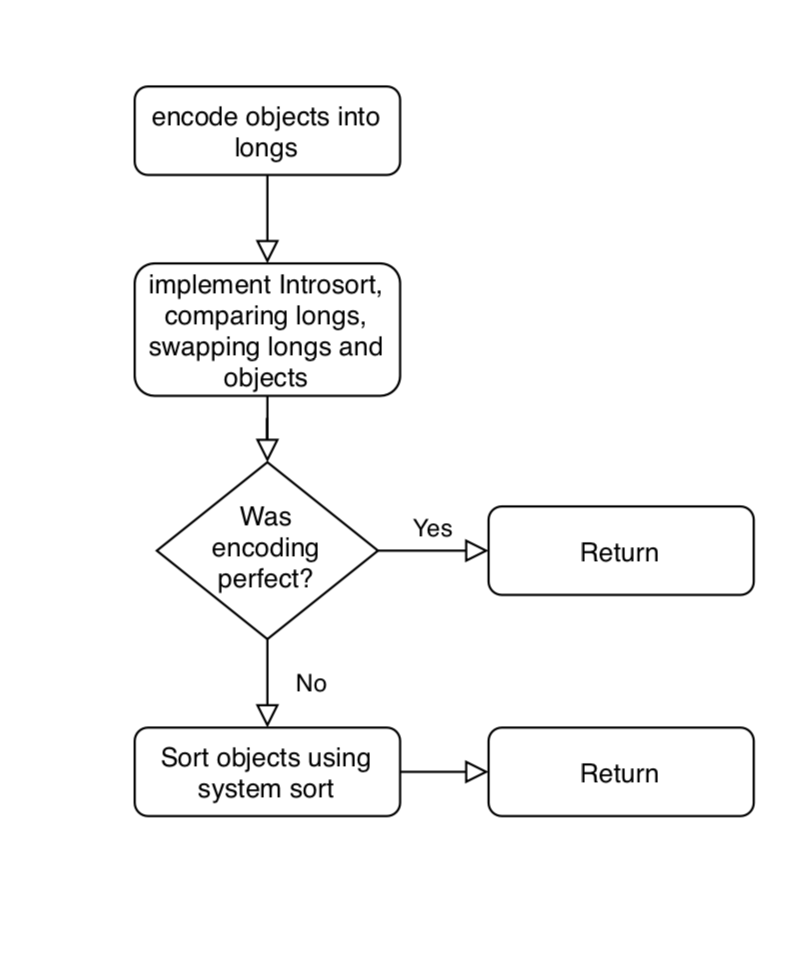
\includegraphics[trim=62 74 22 38, clip, width=0.39\linewidth]{HuskySortFlow.png}
\end{figure}
The strategy of HuskySort (see Flow ~\ref{Fig:HS}) is as follows,
assuming the dataset is presented as an array $xs$ of type $X$:


\begin{steps}
\item  
\renewcommand{\labelenumi}{\alph{enumi}}
    \begin{enumerate}
    \item Create a $long[]$ array (\emph{longs}) of the same size as $xs$;
    \item for each element $x$ of $xs$, set the corresponding element of \emph{longs} to $x.huskyCode()$.
    \end{enumerate}
\item {}Sort array \emph{longs} using quicksort (in practice, we have found that Introsort\cite{doi:10.1002} works well)
in such a way that when elements $i, j$ of \emph{longs} are exchanged, then elements $i, j$ of $xs$ are also exchanged;
\item {}Finally, when quicksort is finished and, if necessary,
we run Timsort on the array $xs$ to ensure that its elements are truly in order.
\end{steps}

For a worked example of a husky coding, see Algorithm ~\ref{alg:permitcoder}

\subsection{RadixHuskySort.}
\label{sec:radix}

Step 2 sorts the husky codes using Introsort, an $\textbf{O}(N log N)$ algorithm,
but the codes themselves are fixed-width 64-bit values,
and radix sort can sort $k$-bit keys in $\textbf{O}(N \cdot \frac{k}{b})$ time using $b$-bit digits —
linear in $N$ for any fixed digit width $b$.
Given that HuskySort's entire premise is to move work from the linearithmic phase to the linear phase,
this raises a natural question we had not previously addressed:
could step 2 itself be made linear? This section describes RadixHuskySort, which we built to answer it (Algorithm ~\ref{alg:the_alg5}).

Radix sort's linear-time advantage rests on a further assumption beyond fixed key width:
that a digit can be turned into an array index in $\textbf{O}(1)$ time,
so that counting and scattering never need to compare two digits directly.
A $b$-bit digit of a husky code satisfies this trivially —
it is extracted by a single shift and mask, and used directly as an index into a $2^b$-bucket counting array.
The original \textit{Comparable} type generally does not:
without first reducing it to such a code, radix sort applied directly to a \textit{String},
a \textit{Tuple}, or a case class would need some other way to decide which of $2^b$ buckets a given key belongs to,
and whenever the natural notion of a "digit" for such a type is not already a small, dense integer,
that decision falls back to \textit{equals} (and, for a hash-based bucket structure,
\textit{hashCode}) on the type itself — an $\textbf{O}(\text{size of the value})$ operation, not an $\textbf{O}(1)$ one.
Husky encoding is what removes this cost from every one of RadixHuskySort's $\frac{64}{b}$ digit passes,
not merely from the final comparison:
once the one-time $\textbf{O}(N)$ encoding step has run,
\textit{equals} and \textit{hashCode} on the original type are not called again until the optional cleanup pass.

A naive adaptation — swapping the object reference alongside each long at every exchange within every digit pass,
exactly as step 2's Introsort swaps at every partition exchange —
would incur $\textbf{O}(N)$ reference movements per digit pass, or $\textbf{O}(N \cdot \frac{64}{b})$ movements in total.
Since $\frac{64}{b}$ is typically much smaller than $log N$ at the sizes we tested,
this would still usually beat Introsort's swap cost,
but it needlessly reintroduces exactly the kind of payload-movement overhead this whole design exists to avoid,
and least-significant-digit (LSD) radix sort's per-pass counting-sort structure makes a better option available.

Instead, RadixHuskySort's step 2 carries only an $\textit{int[]}$ index array through the LSD digit passes,
alongside the (unmodified) long array;
each pass is a stable counting sort keyed on one $b$-bit digit of the (already-computed) husky code,
reordering the index array rather than the codes or the objects themselves.
Once all $\frac{64}{b}$ passes are complete, the index array holds the sorting permutation,
and a single $\textbf{O}(N)$ pass builds the final object array by reading $\textit{xs[index[i]]}$ for each $i$.
This confines all object-reference movement to one pass total, rather than one pass per digit.

Because LSD radix sort's per-digit counting sort treats keys as unsigned,
and husky codes are signed 64-bit values whenever the underlying domain can be negative (e.g., \textit{Integer},
\textit{Long}, or dates before a chosen epoch), each code is first transformed by $\textit{code} \oplus \textit{Long.MIN\_VALUE}$ —
flipping only the sign bit — before the digit passes,
which places negative codes before non-negative ones under unsigned digit comparison without disturbing relative order within either group;
the same transform is idempotent to reverse, so no separate un-flip step is needed once the permutation is built from the transformed codes.
Whether a given \textit{HuskyCoder} can actually produce negative codes is checked rather than assumed,
since several codings (e.g., Unicode strings) never do.

The digit width $b$ is a tunable parameter, trading off the number of passes ($\frac{64}{b}$)
against the size of the per-pass counting array ($2^b$ buckets, which must fit comfortably in cache for each pass to stay fast);
\S~\ref{sec:radix-results} reports how this trade-off plays out empirically across data types and array sizes.
Step 3 (the cleanup pass, run only if the coding is not provably \textit{perfect})
is unchanged regardless of which algorithm sorts the codes in step 2 —
radix sort is a drop-in replacement for that one step, not a change to the overall three-step strategy.

This parameterization also addresses a related limitation:
assuming 64-bit words throughout may not be appropriate for comparison on different key sizes.
Quicksort's asymptotic behaviour does not depend on key width at all —
an $\textbf{O}(N \log N)$ comparison sort costs the same whether the keys being compared are 32 bits or 128 bits wide,
since only the (fixed-cost) comparison itself touches the key's actual bits.
Radix sort, by contrast, makes the key width an explicit, first-class parameter:
a $k$-bit key simply takes $\frac{k}{b}$ passes instead of $\frac{64}{b}$, with no change to the algorithm itself.
So while nothing about the discussion above depends on 64-bit words specifically,
the RadixHuskySort generalizes to other key widths more directly than a comparison-based sort does —
if a future encoding needed, say, 128 bits to capture more of an object's structure,
the same radix sort would apply unchanged, merely with twice as many passes.

Radix sort applied to strings specifically has its own substantial, and older, literature,
distinct from the general fixed-width-key radix sort described above.
Three-way radix quicksort (also called multikey quicksort) and MSD (most-significant-digit)
radix sort for strings were both popularized by Bentley and Sedgewick's classic treatment\cite{314161.314321},
and burstsort\cite{1064546.1180622} improves cache behaviour further by building a small trie to bucket strings before sorting.
These string-specialized algorithms sort variable-length strings directly, character by character, without a separate fixed-width encoding step.
RadixHuskySort's contribution is different in kind, not degree:
it is not a string-sorting algorithm, but a general mechanism applicable to any \textit{Comparable} type
with a 64-bit husky encoding (strings among them),
at the cost of the encoding's own fixed capture window (\S~\ref{sec:pcrit} above)
and a fallback cleanup pass whenever that encoding is imperfect.

That framing carries a consequence which Table ~\ref{tab:RadixImprovements} bears out,
and which we state rather than leave to be noticed:
the string rows of that table are its most variable by a wide margin.
They span from 3.4x down to 1.6x, nearly the whole of its range below dates,
where every other row falls between 2.1x and 3.6x.
Three factors account for the spread, and they compose.
The advantage grows with the cost of the type's native comparison, since that is what the encoding replaces;
it grows with the perfection of the encoding, since an imperfect one is paid for by the cleanup pass;
and it shrinks in the presence of algorithms specialised to the type.
Dates are the favourable extreme on all three counts --- a provably perfect coding, no cleanup pass at all,
and no specialised competitor --- and yield the largest margin in the table at 5.9x.
The string rows show those same three factors varying \emph{within} a single data type,
which is the more instructive demonstration.
Chinese words are favourable on the first two counts --- an expensive Unicode comparison,
captured well enough by the encoding --- and sit fourth of eleven, above all but three of the non-string rows.
Chinese personal names are unfavourable on the second: the comparison is more expensive still,
a table lookup per character, but the pinyin coding captures far less of the key than the Unicode
coding does, so ties are common and the cleanup pass does real work rather than none
(\S~\ref{sec:chinese-coders} accounts for the difference).
The more expensive comparison is paired with the weaker encoding, and this is the weakest result we report.
English words are unremarkable on the first two counts and distinctive on the third,
being the one case in this paper with a mature specialised literature ranged against it.

Strings are unfavourable on the third count in a way no other type in this paper is.
Half a century of specialised string sorting exists,
and a general mechanism should not be expected to beat it on its own ground.
We compared RadixHuskySort against both of the classic string sorts named above,
under JMH, on English and Chinese text, in code-point order so that every sort compared
performs the same task.
Both baselines are our own implementations,
each tuned so that its fallback below the partitioning cutoff allocates nothing
and compares from the depth the partitioning has already established.
Against three-way radix quicksort RadixHuskySort is faster at every size tested,
by 1.3--2.4x on English words and 3.1--4.0x on Chinese words,
with non-overlapping 99.9\% confidence intervals throughout.
Against MSD radix sort the result goes the other way at scale, though not by much:
on English text the two are indistinguishable at $N=32{,}000$,
and MSD is faster by 1.20x at $N=200{,}000$ and by 1.06x at $N=1{,}000{,}000$.
The advantage at $N=200{,}000$ is the robust one.
At $N=1{,}000{,}000$ three runs on the machine of record give 1.00x, 1.05x and 1.06x,
so at the largest size we measure the two algorithms are level to within the spread between runs,
and the direction should be read from the middle size rather than the largest.
We give this result because it locates the boundary rather than obscuring it.
MSD earns it on a corpus that suits it and within limits that are its own:
our implementation indexes an alphabet of 256 characters beyond ASCII,
which English text fits and neither Chinese corpus does,
and it offers no pinyin ordering,
so there is no MSD row for either Chinese corpus.
RadixHuskySort reaches every corpus in this paper through one encoding,
with no per-alphabet provision and no per-type implementation.
That is the claim being made, and the English result bounds it without contradicting it.
A direct empirical comparison against burstsort remains future work;
it is a trie-based, cache-conscious algorithm designed to beat both baselines used here on exactly this workload,
and we have not implemented it.

Code-point order is not a meaningful comparison for Chinese personal names specifically —
it is simply the wrong order for that use case, not merely a different one.
Leaving the word corpus in that order is deliberate: a directory of people has one conventional
ordering and it is by pinyin, where a word list has several --- by radical, stroke count, pinyin or
frequency, according to purpose --- so no single ordering is the right one to hold it to,
and code-point order keeps that row comparable with the English one.
A fair comparison for the names requires a pinyin-aware MultikeyQuicksort.
We extended it with the same syllable-then-tone character key the pinyin encoding of \S~\ref{sec:radix} already uses,
restricted the comparison to the three pinyin-aware sorters, and re-ran it.
RHSort is faster than the repaired multikey quicksort by 1.57x, 1.83x and 2.09x at $N = 32{,}000$,
$200{,}000$ and $1{,}000{,}000$, and QuickHuskySort by 1.33x, 1.49x and 1.27x.
Two independent runs on the machine of record agree to within two hundredths of those multipliers.
Note that the RHSort margin grows with $N$ while QuickHuskySort's does not:
the linear second phase keeps paying as the array grows where a linearithmic one cannot,
which is the same pattern the natural-order corpora show and the clearest form in which this corpus
shows it.

\begin{algorithm2e}
\KwIn{\it{xs} as an array of object X which extends Comparable<X>}
\KwIn{\it{b} as the number of bits per digit}
 coding = huskyCoder.huskyEncode(xs)\;
 longs = coding.longs\;
 index = radixSortIndices(longs, b)\;
 ys = permute(xs, index)\;
 \If{coding.perfect}{return ys\;}
 Arrays.sort(ys)\;
 \caption{RadixHuskySort.sort}
 \label{alg:the_alg5}
\end{algorithm2e}

\begin{algorithm2e}
\KwIn{\it{longs} as an array of long}
\KwIn{\it{b} as the number of bits per digit}
\KwOut{\it{index}, a permutation of $0, \ldots, \textit{longs.length} - 1$ such that
  \textit{longs[index[$\cdot$]]} is sorted}
 biased[i] = longs[i] {\bf XOR} Long.MIN\_VALUE, for each i\;
 index = [0, 1, \ldots, longs.length - 1]\;
 \For{digit = 0 \KwTo (64 / b) - 1}{
 index = stableCountingSortPass(biased, index, digit, b)\;
 }
 \caption{radixSortIndices (LSD, deferred permutation)}
 \label{alg:the_alg6}
\end{algorithm2e}

\subsection{Discussion of Husky Encoding.}

Step 1b requires the definition of a 64-bit hash function (huskyCode) whose properties are as follows:
(refer to Algorithm ~\ref{alg:the_alg2})
\begin{itemize}
                        \item {}If $x = y$, then $x.huskyCode() = y.huskyCode()$;
                        \item {}If $x > y$, then: 
                            \begin{itemize}
                            \item{} either $x.huskyCode() <= y.huskyCode()$ (with probability $p$)
                            \item{} or $x.huskyCode() > y.huskyCode()$ (with probability $1-p$);
                            
                            \end{itemize}
                        
                        \end{itemize}


We interpret this rule as follows:
if $x$ and $y$ are the same ($x.equals(y)$ in Java), their huskyCode should be the same.
If $x > y$, we normally expect that $x.huskyCode() > y.huskyCode()$, i.e., the sort on the husky-coded longs will not invert $x$ and $y$.
However, when $x > y$ while $x.huskyCode() < y.huskyCode()$, then an inversion will be introduced.
And, when $x > y$ and $x.huskyCode() = y.huskyCode()$, then an inversion \emph{may} be introduced because quick-sort is not stable.\cite{6115063}

For a successful encoding, the value of $p$, the probability of a potential inversion, should be less than some critical probability, $p_{crit}$.
Leaving a more detailed discussion of $p_{crit}$ until later, we note that, for some domains of $X$, we can definitely assert that $p = 0$.
We refer to this as a “perfect” encoding.
In such a case, we can skip step 3 of the algorithm because, when $p = 0$, there will be no inversions remaining after quick-sorting according to the huskyCodes.
An example of such a domain is date-time values with a resolution of one nano-second over a period of 128 years.
For strings of English case-independent letters (no punctuation or numbers), i.e., 5-bit ASCII, words of 12 (or fewer) characters in length can also be coded uniquely.
For case-dependent strings (6-bit ASCII), we can encode perfectly if the lengths are all 10 characters or less.
In step 3, it might be acceptable to use insertion sort instead of Timsort.
In any event, assuming that the huskyCode is as accurate as required, then there will be very few inversions (elements out of place) remaining after the quicksort phase.
This implies that the second sort can be performed in very close to linear time.
The results have been very satisfactory.
For example, taking an array of 1,000,000 English words drawn randomly from a corpus of 275,333\cite{GOLDHAHN12.327},
QuickHuskySort sorts in 698 ms against the system sort's 1,121 ms, a factor of 1.61
(for the full data, please refer to table ~\ref{tab:HS_BM}).






\subsection{Discussion of \texorpdfstring{$p_{crit}$}{p\_crit}.}
\label{sec:pcrit}
When $p > 0$, there is a finite probability of any pair of elements remaining inverted after the first sorting pass.
For an array of N randomly ordered elements, the average number of inversions before sorting is $X = N (N -1 ) / 4$.
The number of inversions remaining after the first pass is simply $p X$.
And, for Timsort or insertion sort, the time to re-sort the array will be $t = k (N + p X)$ where $k$ is some system-dependent constant.
The total time to sort the array is made up of these three time-consuming steps where $k_1, k_2, k_3$ are system- and algorithm-dependent constants:

\begin{steps}
 \item{} $T_1$ is the time to encode the elements:
\[T_1 = k_1 N\]
\item{}  $T_2$ is the (average) time to quick-sort the huskyCode array while also swapping the element array itself:
\[T_2 = 2 k_2 N ln N\]
\item{}  $T_3$  is the time to Timsort the element array (only required if $p>0$):
 \[T_3 = k_3 (N + p X)\]
\end{steps}
Provided that the total time $T = T_1 + T_2 + T_3$ is less than the time required to use Timsort on the original element array, we have a win.
This same three-step decomposition ($T_1$/$T_2$/$T_3$, i.e., encode/sort/cleanup) is revisited in \S~\ref{sec:analysis}
in more concrete terms —
counting array accesses directly rather than folding everything into abstract system-dependent constants $k_1, k_2, k_3$ —
and extended there to cover RadixHuskySort (\S~\ref{sec:radix}) as a fourth alternative for the $T_2$ step.
The actual values of $p_{crit}$ are very much dependent on the machine running the sort.
We have not calculated a typical value for $p_{crit}$ but, even for the worst-case:
Chinese characters using UTF8 encoding, we still find very significant gains, reported later in Table ~\ref{tab:HS_BM}.

Of the three terms, $T_3$ can be isolated experimentally.
Two benchmarks over the same two hundred thousand municipal records (\S~\ref{sec:radix-results})
differ only in which coder they are given.
Both compute identical codes; one coder declares itself perfect, so the sort skips step 3,
while the other leaves that declaration at its default and the pass runs.
The encoding for these records is perfect, so the pass that runs has provably nothing to correct.

Its cost is predictable in advance.
Timsort over a fully ascending array detects a single run and stops,
performing $N-1$ comparisons and no moves,
so $T_3$ at $p = 0$ is exactly $N-1$ invocations of the element's own comparator ---
here assessor's block, then lot, then filing date,
which is precisely the comparison the husky encoding was introduced to avoid.
The cleanup pass reintroduces one full composite comparison per element,
having just removed it from all $\textbf{O}(N \log N)$ of them.

That comparison costs 16.1\,ns at $N = 32{,}000$, 60.3\,ns at $N = 100{,}000$ and 74.2\,ns at
$N = 198{,}900$ --- 7.3\%, 17.2\% and 17.3\% of the running time of the sort that contains it ---
with non-overlapping 99.9\% confidence intervals throughout.
Three further runs, one of them on different hardware, agree on the shape at different levels;
across all four the pass costs between a sixteenth and a quarter of the total,
and between a sixth and a quarter at the two larger sizes.
The percentages are the less stable figures, being ratios of two quantities that both move.
The shape is a threshold rather than a trend --- a rise by a factor of roughly three to four between the first two sizes,
then a levelling off --- and it falls where the records stop fitting in cache.
That last reading is inference, but the magnitudes support it:
the system sort compares these same records some 3.5 million times in 151\,ms, or 43\,ns each,
so the cleanup pass at 74\,ns costs nearly twice as much per comparison using the same comparator.
Step 2 permutes references without moving the records,
so a scan sequential in the array is close to random in the heap.

Whether this share must shrink as $N$ grows --- the pass being linear where the sort containing it is
linearithmic --- is a fair question, and \S~\ref{sec:cleanup-scaling} answers it.

Two conclusions follow.
First, $k_3$ is not a constant: it varies more than fourfold across three sizes on one machine,
so no single $p_{crit}$ can be quoted even for one type on one machine.
Second, an encoding which can be declared perfect avoids a cost of up to a quarter of total running
time, where one which cannot must repay it before correcting a single genuine inversion.

\subsection{Why husky coding works.}
\label{sec:why-husky}

The rationale is set out in full by Hillyard et al.\cite{huskysort2020}; we restate only what the rest of
this paper depends on.
A 64-bit word holds enough of most keys to place elements close to their final order, and comparing two
longs costs far less than following two object references and running a type-specific
\textit{compareTo} --- so the encoding trades one $\textbf{O}(N)$ pass for cheaper comparisons throughout
the $\textbf{O}(N \log N)$ one.
The code need not be perfect, only good: whatever inversions it leaves are the cleanup pass's problem, and
\S~\ref{sec:pcrit} measures what they cost.

Perfection has a precise limit for strings.
Packing four 16-bit characters fills the word (Table ~\ref{tab:EncodingConstants} gives the constants for
both string codings), but the packed result is then shifted right by one bit, because any string whose
first character is \texttt{0x8000} or above --- common among CJK characters --- would otherwise set the
sign bit and encode as a negative \textit{long}, corrupting numeric comparison.
The shift costs the least significant bit of a true fourth character; for three characters or fewer that
bit is padding, which is why the Unicode coding is declared \textit{perfect} up to three characters and
not four.

Whether a coding was in fact perfect is known before the cleanup pass runs: a constant-time lookup for
non-sequence types, and for strings a scan that stops at the first string too long to encode perfectly.
Where it was perfect, no inversions remain and the pass is skipped altogether.


\begin{algorithm2e}
\KwIn{\it{xs} as an array of object X}
\KwOut{A new \it{Coding} object}
 result = new long[xs.length]\;
 \For{i = 0 to xs.length}{
 result[i] = huskyEncode(xs[i])\;
 }
 return new Coding(result, perfect())\;
 \caption{huskyEncode}
 \label{alg:the_alg2}
\end{algorithm2e}


\begin{algorithm2e}
\KwIn{\it{permit}, with fields \it{block}, \it{lot}, \it{filedDate}\;}
\KwOut{a 60-bit code, order-preserving for \it{permit.compareTo}}
 \tcp{fields most-significant first, in compareTo order}
 r = encodeString(block, 5, 5, BLOCK\_ALPHABET)\;
 r = r $\ll$ 24 $|$ encodeString(lot, 4, 6, LOT\_ALPHABET)\;
 \Return r $\ll$ 11 $|$ daysSinceEpoch(filedDate)\;
 \BlankLine
 \tcp{codeOf(x, alphabet), used by encodeString for each symbol}
 \eIf{alphabet contains x}{
   \Return 1 + index of x\tcp*{0 is left for padding}
 }{
   \Return count of symbols $<$ x\tcp*{weaken, never invert}
 }
 \caption{A composite husky coder: \textit{PermitCoder}. \textit{encodeString} packs \textit{width}
   symbols of \textit{bits} each, right-padding with zero.}
 \label{alg:permitcoder}
\end{algorithm2e}

\section{Implementation.}

%% ANONYMISATION: the real URL names its owner, so it is guarded with the author block. See
%% "0i. The repository link" in Paper edits pending.md -- the Anonymous GitHub mirror is task 2
%% on Sai Vineeth's list; when its URL exists, substitute it for the placeholder below and the
%% review copy can cite the code directly.
\ifanonymous
  The implementation is available in an anonymised repository, linked from the submission site.
\else
  The implementation is available at \url{https://github.com/rchillyard/HuskySort}.
\fi

\subsection{System Environment.}

Three machines appear in this paper, and \S~\ref{sec:environments} specifies all three.
Machine A ran the JDK 1.8.0\_152 comparison-sort benchmarks of \S~\ref{sec:analysis},
the choice of cleanup sort among them (\S~\ref{sec:cleanup-choice});
machine B, on different hardware and two JVM generations later, ran the radix-sort and JMH development work.
Machine C is the machine of record: an independently administered cloud instance, confirmed idle before
each run, and the source of every figure quoted in this paper.
It is ARM-based like machine B but differs from it in core design, vendor, core count and operating system.

Reporting all three lets a reader check directly whether the qualitative finding generalizes across
machines and JVM versions rather than being an artifact of one environment.
It does: QuickHuskySort, and now RHSort, beat the system sort on all three,
which differ in vendor, instruction set, core design and JVM generation.



\begin{table}
  \caption{String-encoding constants}
  \label{tab:EncodingConstants}
  \begin{tabular}{lll}
    \toprule
    Constant & Unicode & ASCII \\
    \midrule
    Bit width per character & 16 & 7 \\
    Max length (64 / bit width) & 4 & 9 \\
    Mask & \texttt{0xFFFF} & \texttt{0x7F} \\
    \bottomrule
  \end{tabular}
\end{table}

\section{Test Case and Analysis.}

\subsection{Data Source.}
\label{sec:data-source}
The sources for the Strings (English and  Chinese) are retrieved from Leipzig Corpora Collection\cite{GOLDHAHN12.327}.
Chinese personal names, used for the pinyin-order comparisons of \S~\ref{sec:radix-results}, are a separate corpus\cite{wainshine2020chinesenames}.
Every other dataset in this paper is generated: pseudo-random numbers, dates and tuples.
The building-permit records of \S~\ref{sec:radix-results} are not.
They are 198,900 permits filed between January 2013 and February 2018, taken from San Francisco's published
record\cite{sf-building-permits} and ordered by a composite key of assessor's block, lot and filing
date; they are included because their distribution is the city's rather than ours.
Only those three columns are retained, and the data is used under the Open Data Commons Database
Contents License.

In each case, we take data from the appropriate \emph{sentences.txt} file and break it up into strings as shown in Listing~\ref{lst:DS}.


\begin{lstlisting}[caption={Data Source},label={lst:DS},language=Java]
private static String[] getLeipzigWordsFromResource(final String resource) {
    return getWords(resource, HuskySortBenchmark::getLeipzigWords);
}
private static List<String> getLeipzigWords(final String line) {
    return HuskySortBenchmarkHelper.splitLineIntoStrings(line, REGEX_LEIPZIG, REGEX_STRINGSPLITTER);
}
final static Pattern REGEX_LEIPZIG = Pattern.compile("[~\\t]*\\t(([\\s\\p{Punct}\\uFF0C]*\\p{L}+)*)");
public static final Pattern REGEX_STRINGSPLITTER = Pattern.compile("[\\s\\p{Punct}\\uFF0C]");


static List<String> splitLineIntoStrings(final String line, final Pattern lineMatcher, final Pattern stringsplitter) {
    final Matcher matcher = lineMatcher.matcher(line);
    if (matcher.find()) return Arrays.asList(stringsplitter.split(matcher.group(1)));
    else return new ArrayList<>();
}

static String[] getWords(final String resource, final Function<String, List<String>> stringListFunction) {
    try {
        File file = new File(getPathname(resource, DutchHuskySort.class));
        return getWordArray(file, stringListFunction, 2);
    } catch (FileNotFoundException e) {
        logger.warn("Cannot find resource: "+resource, e);
        return new String[0];
    }
}
    } catch (final Exception e) {
        throw new RuntimeException(e);
    }
}


\end{lstlisting}

\subsection{Analysis.}
\label{sec:analysis}
Let’s try to do an analysis of QuickHuskySort's performance.
This expands on the $T_1$/$T_2$/$T_3$ decomposition introduced in \S~\ref{sec:pcrit} above,
replacing its abstract time constants with concrete array-access counts,
and extending it to cover RHSort (\S~\ref{sec:radix}) as an alternative to quicksort for the $T_2$ step.
The first thing to note is that, like merge sort, QuickHuskySort requires $\textbf{O}(N)$ extra space.
This is because, in addition to the array of object references, we must have an equal-length array of longs (the huskyCode values).

Secondly, QuickHuskySort is not stable unless using the merge sort variation.
The derivation of the two comparison figures is a counting argument rather than a measurement, and it
rests on one coefficient we estimated rather than measured; it is set out in \S~\ref{sec:qhs-analysis}.

Encoding's cost has not simply been assumed:
we timed the encoding phase in isolation,
separately from the sort that follows it, to confirm it directly.
At $N = 1{,}000{,}000$, encoding takes 67.7ms for English words (9.7\% of QuickHuskySort's 697.9ms total,
24.8\% of RHSort's 272.7ms) and 211.1ms for Chinese names encoded via pinyin (16.9\% of QuickHuskySort's
1252.7ms, 27.8\% of RHSort's 760.9ms) — confirming that encoding cost, while real and non-negligible,
especially for the more elaborate pinyin encoding, remains a minority of total time in every case measured,
consistent with the linear-and-subordinate role it is assumed to play above.
Encoding's share of the total is larger for RadixHuskySort than for QuickHuskySort in both cases,
simply because RHSort's own contribution to the total is smaller —
as the sort phase gets cheaper,
whatever cost remains in the encoding phase necessarily becomes a proportionally larger slice of what is left,
which suggests encoding cost (particularly for pinyin)
is the more promising target for further optimization now that the sort phase itself is no longer the dominant cost.
The consequence of this is that, as expected,
the linear phase of QuickHuskySort is relatively high for small $N$ but that is soon swamped by the saving of comparisons in the linearithmic phase.
The break-even point is actually a very small value of $N$:
four.
As $N$ increases, we expect the advantage of QuickHuskySort to increase further.
This is generally borne out by the benchmarks.
Please refer to table ~\ref{tab:Comparison}.

The same style of analysis extends naturally to RadixHuskySort (\S~\ref{sec:radix}).
Each of its $\frac{64}{b}$ digit passes touches every element a small constant number of times,
$c$, to bucket it and to record its new position in the (deferred) index array —
with no partitioning or pivot-comparison overhead, and critically, no logarithmic term at all.
Taking $c = 4$ (the same per-exchange cost used for QuickHuskySort's swaps above),
adding the final $\textbf{O}(N)$ pass that applies the resulting permutation to the object array (2 array accesses per element),
and the same encoding cost ($(k+1)N$) and cleanup-pass cost ($(2 + j + 4)pN$,
unaffected by which algorithm sorts the codes in step 2), the total array accesses for RadixHuskySort ($A_r$) come to:
\[A_r = \left(4 \cdot \frac{64}{b} + 2 + k + 1\right) N + (2 + j + 4)pN\]
Using the same illustrative constants as above ($j = 4$, $k = 7$, $p = 0.1$)
and $b = 16$ (four digit passes, near the middle of the digit-width plateau found empirically —
see \S~\ref{sec:radix-results}):
\[A_r = 27 N\]
Table ~\ref{tab:Comparison} extends the earlier comparison with this term.
At $N = 1{,}000{,}000$, $A_r \approx 27{,}000{,}000$ against $A_h \approx 101{,}000{,}000$ and $A_m \approx 161{,}000{,}000$ —
a predicted advantage of roughly 3.7x over QuickHuskySort,
consistent with the 2-4x speedups actually measured (\S~\ref{sec:radix-results}).
The model does predict one caveat:
equating $A_r$ and $A_h$ gives a theoretical break-even around $N \approx 17$,
somewhat higher than QuickHuskySort's own break-even against merge sort ($N = 4$,
above) — because RHSort's per-pass cost has no logarithmic term to shrink relative to at very small $N$.
This crossover is far below every array size actually tested, so it has no practical effect on the results reported here,
but it is worth stating rather than leaving the model looking like radix wins unconditionally at every $N$.
 \begin{table*}
  \caption{Theoretical comparisons (array accesses, dimensionless counts)}
  \label{tab:Comparison}
  \begin{tabular}{rrrrr}
    \toprule
    N  &  N ln N & merge sort & QuickHuskySort & RHSort \\
    \midrule
     4 & 6 & 72 & 72 & 108 \\
     1,000 & 6,908 & 81,439 & 55,075 & 27,000 \\
     1,000,000 & 13,815,511 & 160,878,371 & 101,149,455 & 27,000,000 \\
     1,000,000,000 & 20,723,265,837 & 240,317,557,125 & 147,224,183,132 & 27,000,000,000 \\

    \bottomrule
  \end{tabular}
\end{table*}

Since the final pass of HuskySort will be cleaning up a relatively small number of inversions, does it
matter whether we use insertion sort or Timsort?
Below about 50,000 Strings it makes barely any difference, and insertion sort is sometimes faster;
beyond that Timsort wins out, by a factor of four and a half at $N = 4{,}000{,}000$.
That measurement, and the choice it settles, are in \S~\ref{sec:cleanup-choice}.


\section{Results and Observations.}
\subsection{Benchmarks.}

Table ~\ref{tab:HS_BM} reports absolute sort times for every data type and corpus.
The two radix columns bracket the digit-width plateau of \S~\ref{sec:radix-results}.
Dual-pivot quicksort and a from-scratch quicksort were measured too; they bear on QuickHuskySort
rather than on RHSort, so they are in \S~\ref{sec:comparison-baselines}.

\begin{table*}
  \caption{Sort times by data type (JMH, ms, mean $\pm$ 99.9\% CI). Numeric types at $N=500{,}000$.
    For Chinese names the system-sort column is a system sort performing the same pinyin ordering;
    code-point order is a different and much cheaper task (\S~\ref{sec:radix-results}).}
  \label{tab:HS_BM}
  \begin{tabular}{llllll}
    \toprule
    Data type & N & System sort & QuickHuskySort & RHSort/8 & RHSort/16 \\
    \midrule
    Integer & 500,000 & 121.2$\pm$0.6 & 89.7$\pm$3.5 & 31.2$\pm$0.5 & 25.2$\pm$0.2 \\
    Double & 500,000 & 141.7$\pm$1.3 & 97.8$\pm$3.6 & 34.0$\pm$0.5 & 31.0$\pm$0.3 \\
    Long & 500,000 & 135.8$\pm$1.2 & 97.7$\pm$1.0 & 30.2$\pm$0.2 & 28.6$\pm$0.3 \\
    BigInteger & 500,000 & 208.4$\pm$1.7 & 152.3$\pm$1.7 & 56.9$\pm$0.3 & 54.1$\pm$0.2 \\
    BigDecimal & 500,000 & 262.2$\pm$1.6 & 144.1$\pm$2.1 & 54.1$\pm$0.3 & 52.5$\pm$0.3 \\
    English words & 32,000 & 13.69$\pm$0.19 & 9.72$\pm$0.12 & 4.63$\pm$0.16 & 4.18$\pm$0.16 \\
    & 200,000 & 141.39$\pm$2.59 & 94.74$\pm$2.44 & 55.01$\pm$2.20 & 50.27$\pm$2.51 \\
    & 1,000,000 & 1120.87$\pm$14.43 & 697.88$\pm$16.15 & 355.26$\pm$24.71 & 272.74$\pm$6.46 \\
    Chinese words & 32,000 & 9.78$\pm$0.08 & 5.00$\pm$0.04 & 2.10$\pm$0.03 & 1.89$\pm$0.02 \\
    (code-point order) & 200,000 & 71.34$\pm$0.63 & 30.90$\pm$0.13 & 13.49$\pm$0.15 & 10.85$\pm$0.10 \\
    & 1,000,000 & 447.12$\pm$2.28 & 219.80$\pm$1.99 & 83.25$\pm$2.31 & 65.46$\pm$1.47 \\
    Chinese names & 32,000 & 69.1$\pm$1.4 & 26.6$\pm$0.3 & 24.1$\pm$0.2 & 23.1$\pm$0.3 \\
    (pinyin order) & 200,000 & 526.2$\pm$9.5 & 187.2$\pm$1.0 & 157.0$\pm$1.3 & 154.9$\pm$1.2 \\
    & 1,000,000 & 3112.9$\pm$68.0 & 1252.7$\pm$6.4 & 775.7$\pm$4.2 & 767.2$\pm$14.0 \\
    Tuples & 20,000 & 3.72$\pm$0.01 & 2.79$\pm$0.02 & --- & 1.30$\pm$0.01 \\
    & 100,000 & 23.24$\pm$0.19 & 17.65$\pm$0.16 & --- & 6.82$\pm$0.05 \\
    & 500,000 & 209.53$\pm$7.98 & 142.61$\pm$1.83 & --- & 57.98$\pm$0.76 \\
    \bottomrule
  \end{tabular}
\end{table*}

\subsection{Summary.}
\label{sec:summary}
HuskySort’s target application is the sorting of randomly ordered arrays of objects on the JVM (Java Virtual Machine).
Let’s eliminate the non-use-cases first:
\begin{itemize}
\item {}Partially-ordered arrays:
that’s to say, arrays with only a linear number of inversions as would be the case when adding a relatively small number of records to a large existing index.
For such use cases, Timsort (the Java system sort for objects) would be more suitable.

\item {}Arrays of primitives:
in Java, a clear distinction exists between primitive types (char, byte, short, int, float, long, double) and objects.
Dual-pivot quicksort (the Java system sort for primitives) is already the fastest algorithm for sorting such types.
\end{itemize}
Thus, HuskySort is best for any object array where there’s no expectation of partial ordering.
Typical improvements over Timsort can be read directly off Table ~\ref{tab:HS_BM} above, which gives
absolute times with 99.9\% confidence intervals rather than summary ranges:
1.4--1.8x across the five numeric types at $N=500{,}000$,
1.4--1.6x on English words,
2.0--2.3x on Chinese words,
and 1.3--1.5x on tuples.
Note that the English margin \emph{widens} with array size rather than decaying,
from 1.41x at $N=32{,}000$ to 1.61x at $N=1{,}000{,}000$.

\subsection{Radix Sort Results.}
\label{sec:radix-results}

We benchmarked every data type and corpus covered above using RadixHuskySort (\S~\ref{sec:radix})
in place of Introsort for step 2, using JMH (the Java Microbenchmark Harness, with proper fork isolation and warmup) on JDK 21.

Table ~\ref{tab:RadixImprovements} reports RHSort's advantage over QuickHuskySort as a direct multiplier —
e.g., \textbf{2.9x} means radix took roughly a third as long —
rather than as a percentage, since a percentage figure close to or above 100\% becomes ambiguous about exactly which quantity it is a percentage \emph{of}.

\begin{table*}
  \caption{RHSort's advantage over QuickHuskySort, as a direct multiplier}
  \label{tab:RadixImprovements}
  \begin{tabular}{cll}
    \toprule
    Data Type & N & Advantage over QuickHuskySort \\
    \midrule
    \texttt{Dates} & 20,000 & 5.9x \\
    \texttt{Long} & 500,000 & 3.6x \\
    \texttt{Integer} & 500,000 & 3.6x \\
    \texttt{Strings of Chinese words (code-point order)} & 1,000,000 & 3.4x \\
    \texttt{Double} & 500,000 & 3.2x \\
    \texttt{BigInteger} & 500,000 & 2.8x \\
    \texttt{BigDecimal} & 500,000 & 2.8x \\
    \texttt{Strings of English words} & 1,000,000 & 2.6x \\
    \texttt{Tuples} & 500,000 & 2.5x \\
    \texttt{Building permits (composite key)} & 198,900 & 2.1x \\
    \texttt{Strings of Chinese names (pinyin order)} & 1,000,000 & 1.6x \\
    \bottomrule
  \end{tabular}
\end{table*}

This is worth confronting directly, since a reader might reasonably ask whether either advantage erodes
as $N$ grows: a constant-factor saving on a linearithmic sort could be swamped at scale.
Neither does.
QuickHuskySort's margin over the system sort on English text \emph{widens} with size,
from 1.41x at $N=32{,}000$ to 1.49x and then 1.61x (Table ~\ref{tab:HS_BM}),
and holds roughly constant on both Chinese corpora.
Radix sort's advantage over QuickHuskySort likewise does not shrink with $N$:
at every size and data type in Table ~\ref{tab:RadixImprovements}, the margin is 1.5x or greater,
consistent with the theoretical model of \S~\ref{sec:radix} predicting no logarithmic term at all,
so there is no analogous reason to expect the advantage to erode as $N$ grows further.
The spread across that table is itself informative, and follows the three factors of \S~\ref{sec:radix}.
Chinese names sorted by pinyin order are the smallest margin measured (1.6x),
because both QuickHuskySort and RadixHuskySort must pay the same cleanup pass for a coding
that two or three characters of recurring syllables leave badly imperfect.
Dates show the largest margin (5.9x) because that coding is provably perfect and never needs a cleanup pass at all,
letting RHSort's linear-time advantage show through with nothing else in the way.
The two lie at opposite ends of the same axis: what separates them is not the data type but the perfection of the encoding.

The building permits row is the only one in that table not measured on data we generated:
198,900 real municipal records ordered by a composite key of three fields (\S~\ref{sec:data-source}).
At 2.1x it is tenth of eleven, which is the point worth making about it --- it is not our largest
margin, but it is our largest on data whose distribution we did not choose.
\S~\ref{sec:permits} gives the case study, and \S~\ref{sec:composite-future} what a general
composite encoder would have to provide, that one having been written by hand.

The measurements were reproduced qualitatively on machines A and B of \S~\ref{sec:environments},
which differ from the machine of record and from each other in vendor, instruction set, core design and
JVM generation.
We quote no figures from them, since mixing environments within a comparison would rob it of meaning,
but every ordering reported here holds on all three.

\subsection{Parallel Radix Sort.}
\label{sec:parallel-radix}

Radix sort's digit passes are natural candidates for parallelization (\S~\ref{sec:radix} above).
We implemented and benchmarked a parallel variant:
each pass is split into a configurable number of contiguous chunks, one per worker thread.
Every chunk first computes its own local per-bucket histogram independently, with no synchronization required;
a short sequential step then combines those histograms into an exact starting offset, in the output array,
for every (chunk, bucket) pair — preserving the stability that step 3's cleanup pass, when needed, relies on,
since a chunk's elements always land after all lower-numbered chunks' elements sharing the same bucket;
finally, every chunk scatters its own elements into the output arrays independently,
using only its own precomputed offsets, so no two chunks ever write to the same location.

An initial implementation dispatched the two phases above to a thread pool separately on every pass.
Measurement showed this repeated dispatch itself contributing a real, non-trivial share of the total cost,
particularly at more moderate array sizes.
The overhead was substantially reduced by starting the worker threads once per sort,
rather than once per phase per pass:
each thread runs its own loop over every pass, and the two phases synchronize via reused barriers whose associated actions —
code that runs exactly once per synchronization point, in whichever thread arrives last —
perform the histogram-combine and buffer-swap steps.
Table ~\ref{tab:ParallelRadix} reports the result (\textit{Long[]}, 11-bit digits, milliseconds, mean $\pm$ 99.9\% CI).

\begin{table*}
  \caption{Parallel RHSort:
serial vs. 1, 2, 4, and 8 worker threads}
  \label{tab:ParallelRadix}
  \begin{tabular}{cccccc}
    \toprule
    N & Serial & 1 thread & 2 threads & 4 threads & 8 threads \\
    \midrule
    2,000,000 & 172.0$\pm$5.7 & 165.2$\pm$2.2 & 140.3$\pm$2.0 & 118.5$\pm$2.4 & 109.3$\pm$1.8 \\
    10,000,000 & 935.2$\pm$36.9 & 884.5$\pm$21.6 & 731.6$\pm$19.9 & 687.9$\pm$22.1 & 645.3$\pm$20.9 \\
    \bottomrule
  \end{tabular}
\end{table*}

Isolating parallelism itself, that's to say comparing 1 thread against 4, both paying identical thread-coordination overhead,
gives a statistically resolved speedup at both sizes: 1.39x at $N=2{,}000{,}000$ and 1.29x at $N=10{,}000{,}000$,
with non-overlapping confidence intervals in both cases.
Against the serial implementation the improvement is resolved at both sizes too,
172.0ms to 118.5ms at $N=2{,}000{,}000$ and 935.2ms to 687.9ms at $N=10{,}000{,}000$.
Unlike on the eight-core machine of an earlier draft, scaling does not stop at four threads:
on sixteen uniform cores, eight threads beats four at both sizes with intervals that do not overlap,
reaching 1.51x and 1.37x over a single thread.

That is still well short of linear, and the shortfall is the more interesting number:
an eightfold increase in threads buys between 1.4x and 1.5x,
on hardware with no performance/efficiency asymmetry to account for it.
Two explanations fit, and we cannot separate them without hardware counters.
Each digit pass scatters across the whole array, so the sort may simply be limited by memory throughput,
which extra cores do not supply; and each pass's histogram-combine step is sequential,
running once per synchronization point whatever the thread count,
so it grows as a share of the total as threads are added.
The first would be a property of the machine and the second of the design,
and only the second would survive better hardware.

\subsection{Use-Case Guidance.}
\label{sec:usecase}

\S~\ref{sec:summary} already eliminates two cases outright:
partially-ordered arrays, where Timsort's own adaptivity wins, and arrays of already-cheap-to-compare primitives,
where dual-pivot quicksort is already the fastest option.
For the remaining case — arrays of objects with no expectation of partial ordering —
the decision is governed by the three factors of \S~\ref{sec:radix}
rather than by the size of the array,
and Table ~\ref{tab:Guidance} puts them in the order a practitioner can answer them.
Size enters only once those are settled, and then only near the bottom of the range.

\begin{table*}
  \caption{Which sort to reach for. The situations are ordered by how much they decide, and
    array size settles nothing until all of them are.}
  \label{tab:Guidance}
  \begin{tabular}{p{0.42\textwidth}p{0.24\textwidth}p{0.26\textwidth}}
    \toprule
Your situation & Reach for & Evidence \\
    \midrule
    The ordering is already cheap to evaluate --- primitives, or a single numeric field
      & dual-pivot quicksort & cost of encoding cannot be recouped (\S~\ref{sec:summary}) \\
    The ordering is composite or expensive, \emph{and} the key packs exactly into 64 bits
      & RadixHuskySort; no cleanup pass is required
      & the largest margins we measure: dates 5.9x, building permits 2.1x over QuickHuskySort \\
    The ordering is composite or expensive, but the encoding is imperfect
      & RadixHuskySort, even allowing for the cleanup pass
      & that pass costs a sixth to a quarter past $N=100{,}000$, even with nothing to correct
        (\S~\ref{sec:pcrit}) \\
    A sort specialised to your type already exists
      & use it, if it covers your data
      & on English words a tuned MSD radix sort beats us, though our MSD indexes extended
        ASCII only and cannot sort either Chinese corpus (\S~\ref{sec:radix}) \\
    The data defeats the encoding's capture window --- long shared prefixes, or keys wider than
    the coder can see
      & System sort & every husky variant loses its advantage (\S~\ref{sec:adversarial}) \\
    None of the above settles it, or the keys are strings
      & by array size (\S~\ref{sec:usecase})
      & each sort's fixed setup cost is repaid at a different $N$ \\
    \bottomrule
  \end{tabular}
\end{table*}

Only when all of those are answered does array size matter, and then chiefly at the small end,
where each algorithm's fixed setup cost has not yet been amortized.
For String keys we measured every crossover directly (JMH, English corpus, $N=4$ through $10{,}000$).
System sort is the fastest of the group up to $N=20$, though only narrowly there
(0.462$\mu$s against insertion sort's 0.489$\mu$s).
A plain, binary-search-based insertion sort wins outright from $N=50$ through $N=200$ —
the one regime in this paper where plain insertion sort,
not either HuskySort variant, is the best available choice.
QuickHuskySort takes over between $N=200$ and $N=500$, and remains the best choice up to roughly $N=2{,}000$,
since RadixHuskySort's own fixed setup cost is not yet amortized below that point.
That cost can be read directly off the measurements: RadixHuskySort's time is a near-constant
166$\mu$s floor from $N=4$ to $N=500$, the allocation and initialisation of its counting structures,
which only the linear term begins to dominate past a few thousand elements.
Somewhere between $N=2{,}000$ and $N=10{,}000$ it takes over;
its advantage then grows and holds at every larger size tested (Table~\ref{tab:RadixImprovements}).
Every one of these crossovers shares the same shape:
each successive algorithm carries a larger fixed setup cost that only pays for itself once there is enough work to amortize it against —
the same fixed-vs-variable-cost story \S~\ref{sec:parallel-radix} found one level further down,
where ParallelRHSort's own thread/barrier setup only pays off once there is enough work to divide across threads.
These crossover points were measured only for String keys.
The fixed costs involved are architectural rather than type-specific,
so other key types plausibly show similarly-shaped curves at similar sizes,
though that has not been separately confirmed.

Two further caveats from elsewhere in this paper complete the picture.
If the source data defeats the husky encoding's fixed capture window entirely —
a shared prefix longer than the encoding's own character limit, for instance —
neither QuickHuskySort nor RadixHuskySort helps regardless of $N$ (\S~\ref{sec:adversarial}):
both lose to plain System sort, since the encoding pass becomes pure waste and the mandatory cleanup pass must do all the real work anyway.
And given a large enough workload and spare cores, \textit{ParallelRadixHuskySort}
widens RadixHuskySort's own advantage further still (\S~\ref{sec:parallel-radix}),
provided there is enough total work to amortize its own thread-coordination cost.

\section{Conclusion.}

The original idea behind HuskySort, that's to say QuickHuskySort,
was to shift work from the linearithmic phase of sorting to the linear phase (both the prelude and the postlude)
and effect an overall reduction in array accesses and thus processing time.
\label{sec:conclusion-dp}%
This has been demonstrated such that, when sorting objects rather than primitives,
HuskySort is faster than dual-pivot quicksort wherever the ordering is expensive to evaluate ---
by 1.4x on \textit{BigInteger} and 1.7x on \textit{BigDecimal} (\S~\ref{sec:comparison-baselines}).
On \textit{Integer}, \textit{Double} and \textit{Long}, where a comparison costs almost nothing,
the encoding has nothing to amortise and dual-pivot quicksort is ahead instead, by up to a tenth.
That is the same criterion which governs every other result in this paper,
here separating one group of numeric types from another.
It is faster than Timsort for arrays which are not partially ordered, above a few hundred elements;
below that, Timsort's own tuned handling of small arrays wins instead.
It is especially fast for types whose ordering is composite or expensive to evaluate
and whose keys encode perfectly, where the encoding replaces the whole comparison and no cleanup pass is needed.
Strings are not reliably that case:
they are the one domain with a mature specialised literature of its own (\S~\ref{sec:radix}),
and they are also the most variable, spanning nearly the whole range of our results ---
including the narrowest margin we report, for Chinese personal names in pinyin order.

In the case of RadixHuskySort, the performance improvement is even better for datasets above a few thousand in length.
Of course, in this case, there was no linearithmic phase, so the time savings come, as explained above,
from more bit manipulation and fewer calls to \textit{equals}.

These findings are not an artifact of a single development machine.
The same qualitative pattern held on three environments spanning two CPU vendors and three distinct architectures
(\S~\ref{sec:environments}),
the last a 16-core ARM server instance with no performance/efficiency core split to confound the result.
That same run also settled a question the parallel variant's own results had left open (\S~\ref{sec:parallel-radix}):
its scaling ceiling past a handful of threads is a property of the design itself,
the fixed sequential cost of combining per-thread histograms once per pass,
not an artifact of any one machine's particular mix of core types.

HuskySort's advantage is specific to a particular kind of workload rather than universal, and needs
all three of the following to hold: an array of at least a few hundred elements, growing to a few
thousand before RadixHuskySort's own per-pass setup cost is repaid (\S~\ref{sec:usecase});
no expectation of pre-existing order, which favours Timsort's adaptivity instead (\S~\ref{sec:summary});
and a comparison costing more than a single machine-word check --- strings, arbitrary-precision numbers
and multi-field records, as opposed to \textit{int}, \textit{long} or \textit{double},
where dual-pivot quicksort already wins outright.

%%
%% The acknowledgments section is defined using the "acks" environment
%% (and NOT an unnumbered section). This ensures the proper
%% identification of the section in the article metadata, and the
%% consistent spelling of the heading.
%% Guarded with the author block: naming collaborators identifies the authors as surely as
%% the author block does, so the review copy carries no acknowledgments at all.
\ifanonymous\else
  \section*{Acknowledgments}
  To Darshan Dedhia, Akshay Bhusare, Kartik Kumar for their help with this project.
\fi



%%
%% The next two lines define the bibliography style to be used, and
%% the bibliography file.
\bibliographystyle{siamplain}
\bibliography{sample-base}

%%
%% If your work has an appendix, this is the place to put it.
\appendix
\section{Appendix.}
\subsection{The array-access analysis of QuickHuskySort.}
\label{sec:qhs-analysis}

\S~\ref{sec:analysis} counts array accesses for RHSort and compares the result with QuickHuskySort and
merge sort in Table ~\ref{tab:Comparison}. This section derives the two comparison figures.

It is a counting argument, and one step in it is an estimate rather than a count: the factor of 0.6
below, which stands for the proportion of object-reference swaps whose targets have not already been
fetched into cache. We have not measured it. Everything else here is arithmetic over the operation
counts of the algorithms concerned, and the RHSort figure in \S~\ref{sec:analysis} needs no such
factor --- $4 \cdot 64/b$ digit passes is a count, not an estimate. The comparison should be read as an
order-of-magnitude argument, which is all the paper asks of it; the measurements of
\S~\ref{sec:radix-results} are what carry the result.

How many comparisons and swaps does QuickHuskySort require, on average?
Wild and Nebel's average-case analysis of dual-pivot quicksort\cite{WildNebel12} gives, approximately:
\begin{itemize}
    \item Comparisons: $1.9 N ln N$;
    \item Swaps: $0.6 N ln N$.
\end{itemize}

A comparison reads two array elements, though because one comparand is always the pivot --- already
in hand --- the effective count is closer to one.
Each swap requires 4 array accesses, although again, we will be swapping elements that have already been accessed.
The effective number of (normalized) array accesses is, in total, approximately 4 rather than the expected 3.8 + 2.4.
That is to say, the coefficient of $N ln N$ is approximately 4.
The analysis represented by the table is for dual-pivot quicksort.
\footnote{Note that, since dual-pivot quicksort is not actually implemented in the Java library for Comparable objects,
    we re-implemented the class for objects.}
However, in QuickHuskySort, each swap also must swap the object references.
These will not, in general, have been pre-fetched and so the effective total normalized array accesses ($A$) is approximately:
\[A = 4 + 0.6 * 4 = 6.4\]
Additionally, QuickHuskySort requires $N$ huskyCode constructions.
Each of these requires $k+1$ array accesses where $k$ is proportional to the number of fields contributing to the huskyCode.
For a string,
that will be the number of characters in the string (except that this is limited to a relatively small number according to the encoding).
For ASCII strings, it is nine.
For Unicode strings, it is four.

However, keep in mind that this is linear and, while it can’t be completely ignored,
it doesn't contribute to the overall growth of the complexity.

Once the sort of the codes is complete, we will assume that there are $p N$ remaining inversions,
where $p$ is the probability of an idiogenic (self-inflicted) inversion.
Again, while we should not ignore it completely, it is linear.
The number of array access for the comparisons/swaps to fix these will be $(2 + j + 4) p N$,
where $j$ is the number of fields to be compared to get a result ($j$ is usually smaller than $k$).

So, the total number of array accesses ($A$) for Husky-sorting an array of length $N$ is:
\[A = (6.4 ln N + (2 + j + 4) p + k + 1) N\]
   
Timsort would be hard to analyze in the general case and so we instead analyze merge sort,
which should be approximately the same number of array accesses in the average case.
 
For merge sort, the analysis is much simpler:
the number of comparisons for a randomly ordered array of length $N$ is $N log_2 N$.
Merge sort does not use swaps, \emph{per se}, but instead uses copies.
Assuming that we optimize the extra copying, there will be $N$ copies to get the algorithm started and $N$ per level.
Thus, the number of copies will be $N {log_2 N}$.
Each of these copies requires two array accesses while each comparison requires 2 + j (described above) array accesses.
 
The total number of array accesses ($A$) for merge sort is, therefore:
\[A = (4 + j) N log_2 N + 2 N\]
 
Given that $log_2 N = 1.44 ln N$, and assuming that:

$j = 4$ corresponding to the comparison of two strings that start with the same character but differ in the second character; and

$k = 7$ and $p = 0.1$; then

the totals ($A_m$ for merge sort and $A_h$ for QuickHuskySort) come to:
 \[A_m = 11.5 N ln N + 2 N\]
 \[A_h = 6.4 N ln N + 9 N\]

\subsection{Prior comparison-based sorting algorithms.}
\label{sec:prior-algorithms}

The algorithms reviewed in \S~\ref{sec:background}, with the standard complexity and stability
characteristics referred to there.

\begin{table*}
  \caption{Prior comparison-based sorting algorithms}
  \label{tab:PriorAlgorithms}
  \begin{tabularx}{\textwidth}{llllX}
    \toprule
    Algorithm & Average case & Worst case & Stable & Notes \\
    \midrule
    Insertion sort & $\textbf{O}(N + I)$ & $\textbf{O}(N^2)$ & Yes & $I$ = number of inversions; fast only for small or nearly-sorted $N$ \\
    Merge sort & $\textbf{O}(N \log N)$ & $\textbf{O}(N \log N)$ & Yes & Linearithmic regardless of input order; $\textbf{O}(N)$ extra space \\
    Quicksort & $\textbf{O}(N \log N)$ & $\textbf{O}(N^2)$ & No & In-place, cache-friendly; the quadratic worst case is mitigated in practice (e.g., Introsort's heapsort fallback\cite{doi:10.1002}) \\
    Timsort & $\textbf{O}(N + I)$ to $\textbf{O}(N \log N)$ & $\textbf{O}(N \log N)$ & Yes & Hybrid of merge sort and insertion sort, adaptive to existing ascending/descending runs; more precisely $\textbf{O}(N + N \log p)$ for $p$ runs\cite{DBLP:journals/corr/abs-1805-08612} \\
    \bottomrule
  \end{tabularx}
\end{table*}

\subsection{Benchmark environments.}
\label{sec:environments}

Machine C is the machine of record and the source of every figure quoted in this paper.
Machines A and B appear only as the qualitative cross-checks of \S~\ref{sec:radix-results}, and
machine A additionally supplies the cleanup-sort comparison of \S~\ref{sec:cleanup-choice}.

\begin{table*}
  \caption{The three benchmark environments. Machine A supplies the comparison-sort results of
    \S~\ref{sec:analysis}; machine B the radix-sort and JMH development work; machine C, the machine
    of record, every figure quoted in this paper. Machine C's cache geometry is not exposed to the
    guest, hence the dash; machine B's is given per core cluster, since its two clusters differ and
    the benchmarks run on the performance cores.}
  \label{tab:SysEnv}
  \begin{tabularx}{\linewidth}{lXXX}
    \toprule
    & \textbf{A} --- comparison sorts & \textbf{B} --- development & \textbf{C} --- machine of record \\
    \midrule
    Model & MacBook Pro (MacBookPro14,3) & MacBook (Apple Silicon) & AWS EC2 c7g.4xlarge \\
    Processor & Quad-core Intel Core i7, 2.8 GHz, Hyper-Threading & Apple M1, 8 cores (4 performance + 4 efficiency) & ARM Neoverse V1 (Graviton3), 16 vCPU, 2.6 GHz \\
    Cache & 256 KB L2 per core, 6 MB L3 & Performance cores: 192 KB L1I / 128 KB L1D each, 12 MB shared L2. Efficiency cores: 128 KB / 64 KB, 4 MB shared L2. 128 B line & --- \\
    Memory & 16 GB 2133 MHz LPDDR3 & 16 GB unified & 30 GiB \\
    OS & --- & macOS 26.5.2 & Amazon Linux 2023 \\
    JVM & 1.8.0\_152 & OpenJDK 21.0.10 & OpenJDK 21.0.12 (Corretto) \\
    \bottomrule
  \end{tabularx}
\end{table*}

\subsection{Discussion of coding accuracy.}
It is not essential that coding is perfect for HuskySort to work well.
We have experimented with deliberately throwing off the encoding quite drastically.
If the probability of one of these deliberate mis-codings is less than approximately 25 percent, HuskySort can still save time.
The inference that we can take from this is that it is not critical that encodings are all very good.
We can be confident that we are still saving time up to about one in four errors.

These deliberate errors were tested for Bytes and Integers but not the other generic types.

\subsection{Timsort or insertion sort for the cleanup pass.}
\label{sec:cleanup-choice}

Step 3 needs a stable sort for an array that is nearly ordered already, and both Timsort and insertion
sort qualify.
Below about 50,000 elements the choice barely matters and insertion sort is sometimes marginally
faster; beyond it Timsort wins decisively, by a factor of four and a half at $N = 4{,}000{,}000$.
That is why step 3 uses the system sort.
These figures are from machine A of \S~\ref{sec:environments} and are the paper's only measurements not
taken on the machine of record; they are reported here because the effect is an order of magnitude
larger than any plausible machine difference, and because the choice they settle is a design decision
rather than a result.

\begin{table*}
  \caption{Timsort or insertion sort as the cleanup pass (time in milliseconds)}
  \label{tab:TimvsInsertion}
  \begin{tabular}{ccc}
    \toprule
    N & QuickHuskySort, Timsort cleanup & QuickHuskySort, insertion-sort cleanup \\
    \midrule
    \ 1000&0.14&0.14 \\
\ 2000&0.31&0.30 \\
\ 4000&0.63&0.64 \\
\ 8000&1.46&1.56 \\
\ 16000&3.24&3.19 \\
\ 32000&6.56&6.48 \\
\ 64000&16.85&19.41 \\
\ 125000&47.74&54.90 \\
\ 250000&168.21&167.90 \\
\ 500000&259.37&373.43 \\
\ 1000000&602.08&1202.61 \\
\ 2000000&1234.90&3129.23 \\
\ 4000000&2423.62&11018.19 \\

    \bottomrule
  \end{tabular}
\end{table*}

\subsection{Comparison-sort baselines for the numeric and tuple types.}
\label{sec:comparison-baselines}

Table ~\ref{tab:HS_BM} omits two baselines that were measured alongside the others: dual-pivot
quicksort adapted to objects, and the JDK's own primitive-array sort applied to unboxed values.
Both bear on QuickHuskySort rather than on RHSort, which is why they are here rather than in the
body.
The comparison they support is the one drawn in \S~\ref{sec:conclusion-dp}: husky encoding repays
itself when the ordering is expensive, and not otherwise.

\begin{table*}
  \caption{Two further comparison sorts, measured on the same arrays as Table ~\ref{tab:HS_BM} and
    directly comparable with its System sort and QuickHuskySort columns (JMH, ms, mean $\pm$ 99.9\% CI;
    numeric types at $N=500{,}000$). \emph{Dual-pivot quicksort} is Yaroslavskiy's algorithm
    transcribed for objects, the JDK applying it only to primitives; \emph{quicksort (raw)} unboxes each
    element to a primitive and sorts that array with the JDK's primitive sort, discarding the objects
    rather than permuting them --- no payload to carry, no encoding abstraction and no cleanup pass ---
    and so bounds from below what any husky variant could achieve on these types. It was measured for
    the numeric types only; the final block is the Permit tuple.}
  \label{tab:ComparisonBaselines}
  \begin{tabular}{llll}
    \toprule
    Data type & N & Dual-pivot quicksort & quicksort (raw) \\
    \midrule
    Integer & 500,000 & 82.5$\pm$0.2 & 38.1$\pm$0.1 \\
    Double & 500,000 & 89.6$\pm$0.5 & 42.6$\pm$0.2 \\
    Long & 500,000 & 89.2$\pm$0.6 & 38.2$\pm$0.3 \\
    BigInteger & 500,000 & 209.9$\pm$2.0 & 42.2$\pm$0.1 \\
    BigDecimal & 500,000 & 246.2$\pm$3.7 & 47.6$\pm$0.0 \\
    \midrule
    Tuple & 20,000 & 3.41$\pm$0.09 & --- \\
    & 100,000 & 21.36$\pm$0.48 & --- \\
    & 500,000 & 142.70$\pm$4.98 & --- \\
    \bottomrule
  \end{tabular}
\end{table*}

\subsection{The cleanup pass as \texorpdfstring{$N$}{N} grows.}
\label{sec:cleanup-scaling}

\S~\ref{sec:pcrit} measures the cleanup pass at $p = 0$ and reports a share of total running time that
\emph{rises} with $N$, from 7.3\% to 17.3\%.
One objection should be met head on: the pass is linear where the sort containing it is linearithmic,
so its share is bound to fall as $1/\log N$.

Both are true, because $k_3$ is not settled over this range.
It grows more than fourfold between the smallest and largest sizes measured while $\ln N$ grows by a
fifth, so the cache effect swamps the logarithm completely.
Holding $k_3$ at the value it reaches once the records no longer fit in cache, and growing the rest as
$\ln N$, puts the share at some 16\% at $N = 10^{6}$ and 14\% at $N = 10^{7}$:
the decline is real but logarithmic, and the pass does not become negligible at any size we expect to meet.

That last calculation is a model rather than a measurement.
The sort's own per-element cost also grows faster than $\ln N$ across these three sizes,
and the corpus holds 198,900 records, so the measurement cannot be extended on real data.

\subsection{Building permits: the case study in full.}
\label{sec:permits}

The permits row of Table ~\ref{tab:RadixImprovements} is the case this mechanism is designed for.
The ordering is expensive, since a comparison may have to examine all three fields of the key in turn,
and the key nevertheless packs exactly into 60 bits, so no cleanup pass is required at all.
Algorithm ~\ref{alg:permitcoder} gives the coder.
The date field is the one that depends on the corpus rather than on the schema: eleven bits admit 2,048
consecutive days and the extract spans 1,878, so the coder checks each date against that window and
refuses one outside it rather than encoding it wrongly ---
which is what makes \textit{perfect()} a verified property here rather than an assumption.
The corpus also shows why real data is worth the trouble of obtaining: its published window begins on
1 January 2013 and ends on 25 February 2018, but no permit bears either date, nor any other weekend or
public holiday --- all 198,900 were filed on a business day.
A generated corpus would not have that structure unless someone had thought to put it there.
Against the system sort, RadixHuskySort is faster by 5.17x, 4.26x and 4.53x at $N = 32{,}000$,
$100{,}000$ and $198{,}900$; against QuickHuskySort, by 2.52x, 2.06x and 2.12x.

At 2.1x over QuickHuskySort the row is tenth of eleven.
A composite key of three fields is more expensive to compare than a single \textit{Long} but a good
deal cheaper than a pinyin lookup per character, so the margin falls squarely inside the range the
three factors of \S~\ref{sec:radix} predict for it.
That is the point worth making about it: it is not our largest margin, but it is our largest on data
whose distribution we did not choose, and a mechanism that only worked on synthetic inputs would not be
worth reporting.

The same records also supply the cleanup-pass measurement of \S~\ref{sec:pcrit},
because the encoding for them is perfect and can be declared so ---
which is what allows the pass to be switched on and off over identical codes.

\subsection{Why the two Chinese corpora sit at opposite ends of the table.}
\label{sec:chinese-coders}

Both corpora are Chinese text, yet they sit at opposite ends of Table
~\ref{tab:RadixImprovements}.
The difference is entirely in how the two coders spend their 64 bits.

The Unicode coder gives each character sixteen bits, drawn from a range of thousands of code points,
and a Leipzig Chinese word runs to one to four characters --- so the code often captures the whole word
and the encoding is close to perfect.
The pinyin coder gives each character nine bits for its syllable and two more for its tone, but there
are only a few hundred distinct syllables and five tones, so the entropy available per character is far
below sixteen bits however many are allocated to it.
Names are two or three characters, and their surnames are drawn from a smaller pool again: a few
hundred cover most of the corpus.

Distinct codes are therefore scarce where the Unicode coder has them in abundance, ties are frequent,
and step 3 has genuine work to do rather than none.
The pinyin case pairs the paper's most expensive comparison with its weakest encoding, which is why it
is the smallest margin we report --- and why the two Chinese rows should not be read as two points on a
single axis.

\subsection{Future work: composite keys, and what a library would have to provide.}
\label{sec:composite-future}

The permit coder above was written by hand, as was every composite encoding in this paper.
One practical obstacle stands between that and a library implementation of this mechanism,
and removing it is the piece of future work we think matters most for adoption.
A hand-written coder must satisfy three properties that nothing checks.
Fields must be packed most-significant-first in the same order as the type's own comparison.
Symbol codes must run from one upwards, so that a field shorter than its width pads with zero and
sorts low, as a string prefix does.
And a symbol outside a field's alphabet must collapse to the largest symbol at or below it,
so that an unexpected value weakens the ordering rather than inverting it.

The first of those is the one that bites, and it bites hardest where one might expect it to matter
least.
An encoding declared perfect skips the cleanup pass entirely (\S~\ref{sec:pcrit}),
so if its field order does not match the comparison, the sort returns the wrong answer and nothing
downstream detects it.
The same mistake in an imperfect encoding is merely slow: the cleanup pass re-sorts by the real
comparison and the answer is still correct.
Field order therefore matters most exactly when the encoding is at its best.

We expect most of this can be automated rather than merely assisted.
Where a type's ordering is already derived from its field declarations ---
as with Java records, or Python dataclasses declared with an ordering ---
the encoding can be derived from the same declaration,
which removes by construction the possibility that packing order and comparison order disagree,
and would let the perfection flag be computed rather than asserted and separately verified.
What such a derivation additionally needs is each field's range rather than its type,
since it is the narrowness of the fields that lets a composite key fit at all:
the permit block field is five characters of a thirty-one symbol alphabet, not an unbounded string.
That range is either declared or inferred from the data.

This argues specifically for the radix variant.
Once the fields do not fit in 64 bits --- three fit comfortably, six will not ---
a wider code costs RadixHuskySort proportionally more digit passes and nothing else (\S~\ref{sec:radix}),
where a comparison-based husky sort has no comparable escape.

\subsection{Adversarial inputs.}
\label{sec:adversarial}

The discussion in section A.1 raises a concern:
it may be possible to construct inputs on which the husky encoding has poor entropy,
and it is not obvious in advance how gracefully (or badly) the sort that follows would degrade in that case.
We constructed two such inputs deliberately, to see how the two variants (QuickHuskySort and RadixHuskySort, \S~\ref{sec:radix}) each degrade.

\textbf{Collapsed high-order bits.} We generated arrays of \textit{Long} values with a swept number of high-order bits held identical across every element (the rest random) —
0 fixed bits is the random baseline, 63 leaves only the sign bit free —
and compared against a re-implementation from scratch of dual-pivot quicksort
(the same baseline used for the numeric comparisons above, without any three-way or equal-key handling).
That baseline is reported twice, and the pair is the most informative thing in this section.
Java's own \textit{DualPivotQuicksort} bounds its recursion at 64 levels and falls back to heapsort beyond it;
our transcription of the algorithm originally did not.
Table ~\ref{tab:AdversarialBits} reports both, at $N = 1{,}000{,}000$.

\begin{table*}
  \caption{Timings (ms) as high-order bits are progressively collapsed, $N = 1{,}000{,}000$.
    The dual-pivot baseline is shown both without a recursion-depth bound and with the one the JDK
    itself applies.}
  \label{tab:AdversarialBits}
  \begin{tabular}{cccccc}
    \toprule
    Fixed high bits & System sort & QuickHuskySort & \multicolumn{2}{c}{Dual-pivot quicksort} & RHSort/16 \\
     & & & unguarded & guarded & \\
    \midrule
    0  & 477.6 & 420.0 & 335.7 & 335.9 & 74.8 \\
    32 & 493.8 & 420.8 & 340.9 & 331.2 & 69.6 \\
    48 & 485.1 & 357.9 & 354.6 & 333.3 & 66.8 \\
    56 & 174.3 & 197.8 & \textbf{7097.7} & 717.2 & 58.9 \\
    60 & 115.9 & 69.8  & \textit{stack overflow} & 805.5 & 42.6 \\
    63 & 42.6  & 15.4  & \textit{stack overflow} & 186.9 & 34.9 \\
    \bottomrule
  \end{tabular}
\end{table*}

Radix sort's timings stay essentially flat across the entire sweep, exactly as the model of \S~\ref{sec:radix} predicts:
each digit pass does the same fixed amount of work regardless of how the keys are distributed,
so a pass over collapsed digits (everything lands in one bucket) costs no more than any other pass.

The unguarded baseline degrades by more than an order of magnitude at 56 fixed bits and then fails
outright, exhausting the stack at 60 and 63.
This is a well-known failure mode for a quicksort that partitions naïvely around a heavily-duplicated pivot value:
Bentley and McIlroy's classic treatment of engineering a practical quicksort\cite{10.1002/spe.4380231105}
specifically addresses this case (a solution to Dijkstra's Dutch National Flag problem, partitioning into three regions — less than, equal to,
and greater than the pivot — rather than two), precisely to avoid the pathological recursion depth this baseline exhibits.
The degradation is far worse than the crash makes it look, because the crash truncates it.
Removing the stack limit rather than the recursion, and timing the same input at $N=1{,}000{,}000$ with the
depth bound raised until it never fires, gives 363 seconds at 63 fixed bits against 0.4 seconds at none —
a factor of nine hundred, on data of identical size.

The guarded column is the same algorithm with the bound the JDK ships, and it is a different story
entirely: nothing crashes, and the 21x degradation at 56 fixed bits becomes 2.1x.
What that column is measuring, however, is largely \emph{not} quicksort.
On these inputs the partitions go unbalanced immediately, the bound is reached within the first few dozen
levels, and heapsort finishes the work.
The clearest evidence is the direction of the sweep: unguarded, the worst case is 63 fixed bits, the most
degenerate input, which is what the partitioning pathology predicts; guarded, 63 is the \emph{fastest}
cell in the row.
The guard has not made dual-pivot quicksort robust here.
It has detected that dual-pivot quicksort cannot cope and changed algorithm, which is what a
production sort should do and is worth stating plainly, since a reader may otherwise take the guarded
column for evidence that the pathology is mild.

QuickHuskySort neither crashes nor slows down anywhere in this sweep — if anything it gets faster as duplication increases,
the same pattern System sort shows,
consistent with Timsort's adaptive run-detection treating long runs of nearly equal keys as already sorted.
Indeed both overtake RHSort at the extreme of the sweep,
where 63 fixed bits leave almost nothing to sort and an adaptive algorithm has almost nothing to do,
while radix still pays for its fixed number of passes.
Radix sort's robustness is of a third kind, and the most useful of the three:
it needs neither an adaptive algorithm's luck with the input nor a fallback to a different algorithm,
because its cost does not depend on the distribution at all.
It is the only sort here whose worst case can be read off its best.

\textbf{Shared string prefixes.}
We took real corpus words and prepended a fixed-length prefix of repeated characters,
long enough in the worst case to exceed the English coder's character-capture window (nine 7-bit ASCII characters per 64-bit code).
Table ~\ref{tab:AdversarialPrefix} reports timings at $N = 1{,}000{,}000$.

\begin{table*}
  \caption{Timings (ms) as a shared string prefix grows, $N = 1{,}000{,}000$}
  \label{tab:AdversarialPrefix}
  \begin{tabular}{cccc}
    \toprule
    Prefix length & System sort & QuickHuskySort & RHSort/16 \\
    \midrule
    0  & 1351.6 & 583.4 & 234.4 \\
    10 & 862.1 & 867.0 & 873.0 \\
    20 & 861.7 & 912.7 & 904.1 \\
    40 & 887.6 & 944.0 & 967.4 \\
    \bottomrule
  \end{tabular}
\end{table*}

This is a genuinely different failure mode, and a less flattering one.
Once the shared prefix reaches the coder's nine-character window, every element's husky code becomes bit-for-bit identical —
the encoding provides zero disambiguation — and \emph{every} Husky-based approach,
radix included, loses its advantage completely,
finishing level with plain System sort or a little behind it rather than ahead.
The mechanism has nothing to do with which algorithm sorts the codes in step 2:
once the encoding carries no information at all,
the entire ordering burden falls on the mandatory cleanup pass (step 3) doing real string comparisons —
comparisons that are themselves more expensive than usual,
since they must scan past the shared prefix before finding a difference —
and whichever algorithm ran first in step 2 did genuinely useless work before that.
Radix does not recover any advantage here, and is very slightly the slowest of the three Husky-based options in this regime,
since its fixed per-pass cost (a strength above) becomes pure overhead once there is no information left to sort.

Taken together, these two experiments answer the question posed above with two distinct results.
When keys collide in their high-order bits but the encoding itself is still informative,
RHSort is effectively immune, and a comparison sort is not:
unguarded it degrades by orders of magnitude or fails outright,
and guarded it survives only by abandoning the algorithm one asked for.
But when the source data overwhelms the encoding's fixed capture window entirely, no choice of sort algorithm for the encoded longs helps at all;
this is a limitation of the fixed-width encoding scheme itself, not of HuskySort's algorithmic strategy,
and it is already implicit in the $p_{crit}$ discussion of \S~\ref{sec:pcrit}:
whenever the actual input defeats the encoding,
the result is that no downstream sort algorithm can recover the information the encoding failed to capture.

Worth noting as a related, if incidental, finding:
the three-way radix quicksort baseline used in \S~\ref{sec:radix} for the classic string-sorting-literature comparison (MultikeyQuicksort)
shares exactly the same failure mode as the naive quicksort baseline above, for a similar structural reason.
Its equal-partition recursion advances one level per shared prefix character;
on a long enough run of strings sharing a common prefix — the same kind of adversarial construction as above —
a straightforward recursive implementation consumes one stack frame per shared character and eventually overflows the stack.
Unlike the failure discussed above, this is a property of the comparison algorithm itself and unrelated to Husky encoding.
We fixed it in our own implementation by converting that one recursive call into a loop,
restoring constant stack depth regardless of prefix length.

The MSD radix sort baseline needs a comparable fix, for a different reason.
A run of equal strings occupies a single bucket at every depth beyond their length,
so recursion into that bucket reduces neither the range nor the work outstanding.
The cutoff to insertion sort conceals this below its own threshold,
and a corpus sampled with replacement exceeds that threshold at scale.
All three of the comparison baselines discussed here therefore carried an unbounded-recursion failure mode,
and all three have now been repaired: the multikey recursion converted to a loop, the MSD cutoff corrected,
and the dual-pivot baseline given the depth bound the JDK applies.
Only the third of those changes what the sweep reports, which is why it is shown both ways.
RadixHuskySort was never at risk of any of them in the first place,
since LSD radix sort has no recursion to begin with.

\subsection{Handling of partially-sorted arrays.}

Not surprisingly, QuickHuskySort is best suited for sorting random arrays.
The benefits of partially-sorted arrays are enjoyed most by the merge sort family of algorithms (including Timsort).
However, we have studied the efficacy of a modified merge sort (it is required to manage both the objects and the longs) as the first pass of the algorithm.
For random English String inputs,
the merge-sort variation improves on the system sort by approximately 20 percent, where the normal Introsort-based QuickHuskySort improves on it by more like 40 percent.

However, neither husky variant is recommended when arrays are partially ordered.
In such cases, the merge-sort variation of QuickHuskySort will take between one and a half and four times as long as Timsort.

\end{document}
\endinput
%%
%% End of file `sample-acmtog.tex'.
"  -> blind, no stamp
%%
%% paper/build.sh builds both.
\newif\ifanonymous
\ifdefined\ANONYMOUS \anonymoustrue \else \anonymousfalse \fi

\newif\ifdraftstamp
%% The stamp is a build timestamp, which is exactly the sort of incidental metadata that is
%% better absent than explained under double-blind review -- so it follows the anonymity flag
%% rather than being switched by hand and forgotten.
\ifanonymous \draftstampfalse \else \draftstamptrue \fi
%% \time is TeX's minutes since midnight, in local time -- verified against the system clock,
%% timezone and DST offset all agreeing.
%%
%% NOTE the division must be done with \divide, not \numexpr. \numexpr ROUNDS rather than
%% truncating, so \numexpr\time/60 gives the *next* hour from half past onwards, and the paired
%% minute expression then goes negative: a 08:35 build stamped itself "09:0-25". Hence counters.
%% Plain names, not hs@ ones: @ is not a letter in a document preamble, so \hs@stamphr would
%% tokenize as two control sequences and the definition below would fail.
\newcount\hsstamphr \newcount\hsstampmin \newcount\hsstamptmp
\newcommand{\revisionstamp}{%
  \hsstamphr=\time \divide\hsstamphr by 60
  \hsstamptmp=\hsstamphr \multiply\hsstamptmp by 60
  \hsstampmin=\time \advance\hsstampmin by -\hsstamptmp
  \the\year-\ifnum\month<10 0\fi\the\month-\ifnum\day<10 0\fi\the\day\space
  \ifnum\hsstamphr<10 0\fi\the\hsstamphr:\ifnum\hsstampmin<10 0\fi\the\hsstampmin}
%%
%% Submission ID.
%% Use this when submitting an article to a sponsored event. You'll
%% receive a unique submission ID from the organizers
%% of the event, and this ID should be used as the parameter to this command.
%%\acmSubmissionID{123-A56-BU3}

%%
%% The majority of ACM publications use numbered citations and
%% references.  The command \citestyle{authoryear} switches to the
%% "author year" style.
%%
%% If you are preparing content for an event
%% sponsored by ACM SIGGRAPH, you must use the "author year" style of
%% citations and references.
%% [acmart-only] \citestyle{acmauthoryear}
% \documentclass{article}
\usepackage{enumitem}
\usepackage[algo2e, boxruled, linesnumbered, noend, noline]{algorithm2e}
\newlist{steps}{enumerate}{1}
%% The label is a whole word, so it needs a labelwidth to match. Without one, enumitem hangs
%% it to the LEFT of the list's text block, and in siamproceedings' narrower column that put
%% "Step 1:" across the gutter and over the neighbouring column. leftmargin=! makes enumitem
%% derive the margin from labelwidth + labelsep, so the label stays inside the column.
\setlist[steps, 1]{label = Step \arabic*:, align = left,
                   labelwidth = 4em, labelsep = 0.5em, leftmargin = !}
\usepackage{listings}
\usepackage{graphicx}
\usepackage{latexsym}
\usepackage{etoolbox}
\usepackage{academicons}
\usepackage{tabularx}


%New colors defined below
\definecolor{codegreen}{rgb}{0,0.6,0}
\definecolor{codegray}{rgb}{0.5,0.5,0.5}
\definecolor{codepurple}{rgb}{0.58,0,0.82}
\definecolor{backcolour}{rgb}{0.95,0.95,0.92}

%Code listing style named "mystyle"
\lstdefinestyle{mystyle}{
  backgroundcolor=\color{backcolour},   commentstyle=\color{codegreen},
  keywordstyle=\color{magenta},
  numberstyle=\tiny\color{codegray},
  stringstyle=\color{codepurple},
  basicstyle=\ttfamily\footnotesize,
  breakatwhitespace=false,         
  breaklines=true,                 
  captionpos=b,                    
  keepspaces=true,                 
  numbers=left,                    
  numbersep=5pt,                  
  showspaces=false,                
  showstringspaces=false,
  showtabs=false,                  
  tabsize=2
}

%------------------------------------------------------------------------------
% Code for ORCID iD
%------------------------------------------------------------------------------
\begin{comment}
% Make Orcid icon
\definecolor{lime}{HTML}{A6CE39}
\DeclareRobustCommand{\orcidicon}{
	\begin{tikzpicture}
	\draw[lime, fill=lime] (0,0) 
	circle [radius=0.16] 
	node[white] {{\fontfamily{qag}\selectfont \tiny ID}};
	\draw[white, fill=white] (-0.0625,0.095) 
	circle [radius=0.007];
	\end{tikzpicture}
	\hspace{-2mm}
}

\foreach \x in {A, ..., Z}{
	\expandafter\xdef\csname orcid\x\endcsname{
	    \noexpand\href{
	        https://orcid.org/\csname orcidauthor\x\endcsname
	        }
	    {\noexpand\orcidicon}
	}
}

% Define the ORCID iD command for each author separately.
\newcommand{\orcidauthorA}{0000-0001-5446-5645}
\newcommand{\orcidauthorB}{0000-0002-5538-8378}
\newcommand{\orcidauthorC}{0000-0001-9734-7358}
\end{comment}
%%
%% end of the preamble, start of the body of the document source.



%"mystyle" code listing set
\lstset{style=mystyle}

\date{ }

\begin{document}

%%
%% The "title" command has an optional parameter,
%% allowing the author to define a "short title" to be used in page headers.
\title{RadixHuskySort: A Linear Second Phase for Proxy-Key Sorting}

%%
%% The "author" command and its associated commands are used to define
%% the authors and their affiliations.
%% Of note is the shared affiliation of the first two authors, and the
%% "authornote" and "authornotemark" commands
%% used to denote shared contribution to the research.
%% \author[R C HILLYARD]{R C HILLYARD\orcidA{}}
%% ---- Authors -------------------------------------------------------------------------
%% SIAM's form (example_doublecolumn.tex): affiliations go in \thanks footnotes, and the
%% second author shares the first's via \footnotemark.
%%
%% ANONYMISATION (see "0k. The front matter" in Paper edits pending.md): the review copy must
%% carry no names, emails, affiliations or ORCIDs. Rather than keep a second copy of this file,
%% the block is guarded -- build with \def\ANONYMOUS{} to suppress it. EasyChair still collects
%% the real author metadata; anonymising *that* would be a mistake.
\ifanonymous
  \author{}
\else
  \author{R C Hillyard\thanks{College of Engineering, Northeastern University, 360 Huntington
      Avenue, Boston, Massachusetts 02115, USA (\email{r.hillyard@northeastern.edu},
      \email{liaozheng.y@northeastern.edu}, \email{kandappareddigari.s@northeastern.edu}).}
    \and Yunlu Liaozheng\footnotemark[1]
    \and Sai Vineeth K R\footnotemark[1]}
\fi



%%
%% By default, the full list of authors will be used in the page
%% headers. Often, this list is too long, and will overlap
%% other information printed in the page headers. This command allows
%% the author to define a more concise list
%% of authors' names for this purpose.

%%
%% The abstract is a short summary of the work to be presented in the
%% article.


%%
%% The code below is generated by the tool at http://dl.acm.org/ccs.cfm.
%% Please copy and paste the code instead of the example below.
%%
%% \begin{CCSXML}
%% <ccs2012>
%%    <concept>
%%        <concept_id>10003752.10003809.10010031.10010033</concept_id>
%%        <concept_desc>Theory of computation~Sorting and searching</concept_desc>
%%        <concept_significance>500</concept_significance>
%%        </concept>
%%    <concept>
%%        <concept_id>10003752</concept_id>
%%        <concept_desc>Theory of computation</concept_desc>
%%        <concept_significance>300</concept_significance>
%%        </concept>
%%    <concept>
%%        <concept_id>10011007.10011006.10011008.10011024.10011028</concept_id>
%%        <concept_desc>Software and its engineering~Data types and structures</concept_desc>
%%        <concept_significance>500</concept_significance>
%%        </concept>
%%    <concept>
%%        <concept_id>10010520.10010521.10010528.10010536</concept_id>
%%        <concept_desc>Computer systems organization~Multicore architectures</concept_desc>
%%        <concept_significance>100</concept_significance>
%%        </concept>
%%    <concept>
%%        <concept_id>10003752.10010070.10010111.10011710</concept_id>
%%        <concept_desc>Theory of computation~Data structures and algorithms for data management</concept_desc>
%%        <concept_significance>500</concept_significance>
%%        </concept>
%%  </ccs2012>
%% \end{CCSXML}

%% [acmart-only] \ccsdesc[500]{Theory of computation~Sorting and searching}
%% [acmart-only] \ccsdesc[300]{Theory of computation}
%% [acmart-only] \ccsdesc[500]{Software and its engineering~Data types and structures}
%% [acmart-only] \ccsdesc[100]{Computer systems organization~Multicore architectures}
%% [acmart-only] \ccsdesc[500]{Theory of computation~Data structures and algorithms for data management}
%%
%% Keywords. The author(s) should pick words that accurately describe
%% the work being presented. Separate the keywords with commas.
%% [acmart-only; siamproceedings has no \keywords. Kept because EasyChair and the
%% camera-ready both want this list.]
%% \keywords{Sorting, Quicksort, Timsort, Radix sort, Complexity, Comparison Sorting, String sorting, Parallel sorting}
\maketitle

\begin{abstract}
    A common computational model for sorting algorithms is based on the numbers of comparisons and/or exchanges they perform.
    We argue that a better yardstick is the total number of array accesses,
    which, for a divide-and-conquer sort, falls into a linearithmic phase and possibly a linear one:
    moving work out of the first and into the second reduces the total.
    This is particularly true where comparison itself is expensive likely leading to a reduction in running time as well.
    The mechanism we present is based a 64-bit code, order-preserving as far as possible,
    that stands as a proxy for each element; we call it a husky code.
    Its effect is to extract each element's sort key once, or at most twice, rather than at each level of recursion.
    Earlier work sorted such codes with quicksort.
    We replace that with a linear-time radix sort, making the second phase linear too,
    and describe a parallel variant of it.
    Measured against Java's system sort for objects --- integers, arbitrary-precision numbers,
    dates, tuples, English and Chinese text, Chinese personal names in pinyin order,
    and, by way of example, a large number of municipal records ordered by a composite key ---
    RadixHuskySort is faster in every case, by 3.6x to 6.8x at the largest size measured for each.
    The margin is widest where the ordering is expensive to evaluate and the encoding is perfect;
    and where the encoding is imperfect we measure directly what the resulting cleanup pass costs.
    One specialised competitor overtakes us: on English words a tuned MSD radix sort.
\end{abstract}


%% siamproceedings loads fancyhdr and empties every header and footer field, so a page number
%% has to be put back explicitly. \maketitle sets the first page to the same style, so this
%% covers page one too and needs no \thispagestyle companion.

\fancyfoot[C]{\thepage}
%% The stamp sits in the right-hand footer field, so it cannot shift the centred page number.
\ifdraftstamp
  \fancyfoot[R]{\footnotesize\itshape draft \revisionstamp}
\fi
%%
%% This command processes the author and affiliation and title
%% information and builds the first part of the formatted document.


\section{Introduction.}
With the vast increase in the size of the data world, efficient computing algorithms play a crucial role in processing data.
From the earliest days of computing,
sorting has been one of the most studied areas of research even though it appears to be a straightforward and familiar topic.
And for good reason.
Binary search, which depends on sorting, is perhaps the most significant optimization technique that systems can use.
The rise of data volume and complexity has increased the need for new approaches to traditional sorting techniques.
Within the realm of comparison-sort algorithms, many aspects of the algorithm can be significant:
stability, adaptability, extra memory, partitioning, merging, exchanging (swapping), copying, and, of course, the comparison itself.

Counting memory operations rather than only comparisons is itself an established idea,
and we frame our own array-access model relative to two well-known lines of work in that tradition rather than proposing it as new:
the external-memory (I/O) model of Aggarwal and Vitter \cite{10.1145/48529.48535},
which counts block transfers between disk and memory, and the cache-oblivious algorithms of Frigo et al. \cite{814600},
which achieve near-optimal memory-hierarchy behaviour without advance knowledge of cache parameters;
and, closest to our own concern, LaMarca and Ladner's study of how caches shape the relative performance
of sorting algorithms\cite{LAMARCA199966}.
Our array-access count is a simpler, single-level analogue of the same underlying idea:
rather than modeling an explicit multi-level memory hierarchy, we count raw array reads and writes as a proxy for real cost,
motivated by the observation that a comparison between two heavyweight objects (e.g., two \textit{String}s)
touches more memory — and likely non-cached memory — than a comparison between two 64-bit primitives.
That observation is orthogonal to, not a substitute for, the external-memory and cache-oblivious literature,
which is chiefly concerned with data too large to fit in memory (or in cache) at all,
rather than with the comparison cost of individual elements that do fit.
Separately, radix sort's independent per-digit counting-sort passes are well suited to parallelization across CPU threads,
a property that is already established for radix sort generally;
\S~\ref{sec:parallel-radix} describes and benchmarks a parallel variant of RadixHuskySort (\S~\ref{sec:radix}).
We do not make an equivalent claim for QuickHuskySort's own comparison-based steps:
Introsort's partitioning and Timsort's adaptive run-detection are both substantially more data-dependent (less independent) and sequential
in character than radix sort's fixed per-digit passes,
so parallelizing them well is a separate, harder problem that this paper does not address.

While sorting appears to be a settled topic, yet new improvements are occasionally made:
\cite{Dual-pivot,Timsort,doi:10.1137/1.9781611975994.101,10.5555/313559.313859,10.1002/spe.4380231105}.
Consequently, there is an abundance of sorting techniques suitable for a myriad of different use cases.
Nevertheless, there is still room for improved versions in regard to computation, memory, time, and space complexity.
In a recent paper\cite{sort}, the authors conclude that quicksort is indeed the fastest general-purpose sorting algorithm,
especially when appropriate care is taken to avoid the quadratic worst-case with several other improvements
(e.g., dual-pivot quicksort)\cite{Dual-pivot} over the traditional version\cite{10.1145/366622.366644}.
However, quicksort does not perform as well as some variations of merge sort, especially Timsort\cite{Timsort}, when the dataset is partially sorted.
Timsort, a hybrid stable sorting algorithm derived from merge sort, is now available in the Python and Java libraries as the default object-sorting utility.

The husky code was introduced by Hillyard et al.\cite{huskysort2020}, together with QuickHuskySort,
which sorts an array of objects by sorting an array of their codes and then repairing whatever the codes
got wrong.
That work established the basic result --- encoding pays for itself for types whose ordering is expensive
to evaluate, among them \emph{String}, \emph{LocalDateTime}, \emph{BigInteger}, \emph{BigDecimal} and many
user-defined types of the same kind --- and it is the starting point of this paper rather than its
subject.
Two things it left undone define the work here.
It sorted the codes with a comparison sort (step 2 of \S~\ref{sec:overview}), so the
$\textbf{O}(N \log N)$ term survived the encoding intact --- the comparisons became cheap, but there
were still $N \log N$ of them.
And while it measured the cleanup pass in one respect, choosing between Timsort and insertion sort for
it (\S~\ref{sec:cleanup-choice}), it did not measure what that pass costs: of $p_{crit}$, the quantity
that governs the cost, it says plainly that no typical value had been calculated.
The contributions here are RadixHuskySort, or RHSort (\S~\ref{sec:radix}),
which replaces that algorithm's comparison sort with a linear-time radix sort on the same codes,
and a parallel variant of it (\S~\ref{sec:parallel-radix});
an empirical comparison against the classic string sorts rather than a theoretical one (\S~\ref{sec:radix});
a direct measurement of the cost of the cleanup pass (\S~\ref{sec:pcrit});
and a case study on real rather than generated data (\S~\ref{sec:radix-results}).
All results reported here were measured anew.

We review existing methods of sorting in Section 2 and go through the HuskySort algorithm in Section 3.
Implementation options and their likely impact are explored in Section 4.
We describe our Test Cases in Section 5 and present results in Section 6, with outcomes summarized in Section 7.


\section{Background.}
\label{sec:background}

Two comparison sorts bracket the design space, and HuskySort's three-step strategy follows from the
contrast between them.
Quicksort is fastest in practice on unordered data, its in-place partitioning and sequential access
outweighing merge sort's guaranteed bound, but it is unstable and its worst case is quadratic unless
mitigated --- as Introsort does, by falling back to heapsort past a recursion-depth
threshold\cite{doi:10.1002}.
Timsort takes the opposite trade: guaranteed $\textbf{O}(N \log N)$ and stable, at the cost of extra
space and of being no faster than $\textbf{O}(N \log N)$ on unordered input, but adaptive, so where the
number of inversions $I$ is small its cost falls towards $\textbf{O}(N)$.
Husky coding exploits both ends of that contrast.
Step 2 hands its sort cheap-to-compare, effectively unordered longs, which is quicksort's best case and,
as \S~\ref{sec:radix} shows, a radix sort's natural input; step 3 hands Timsort an array already close to
sorted, the one regime in which its adaptivity pays.
Standard complexity and stability characteristics for the algorithms named here are tabulated in
\S~\ref{sec:prior-algorithms}.

\section{Algorithm.}





\subsection{Overview.}
\label{sec:overview}

\begin{figure}
  \caption{HuskySort Flow}
  \label{Fig:HS}
   %% [acmart-only] \Description{An Overview of HuskySort}
  \centering
  %% The source PNG carries wide blank margins -- 25\% of its height, 23\% of its width. Measured
  %% ink bounding box is x 133..755, y 85..817 of 806x976 px; pHYs declares 144 dpi, so trim is in
  %% bp (px * 72/144), held a little inside the measured margins so no ink is clipped.
  %% Width is 0.39 rather than 0.5 so that the diagram keeps its original apparent size and the
  %% saving comes out of the blank margin, not out of legibility.
  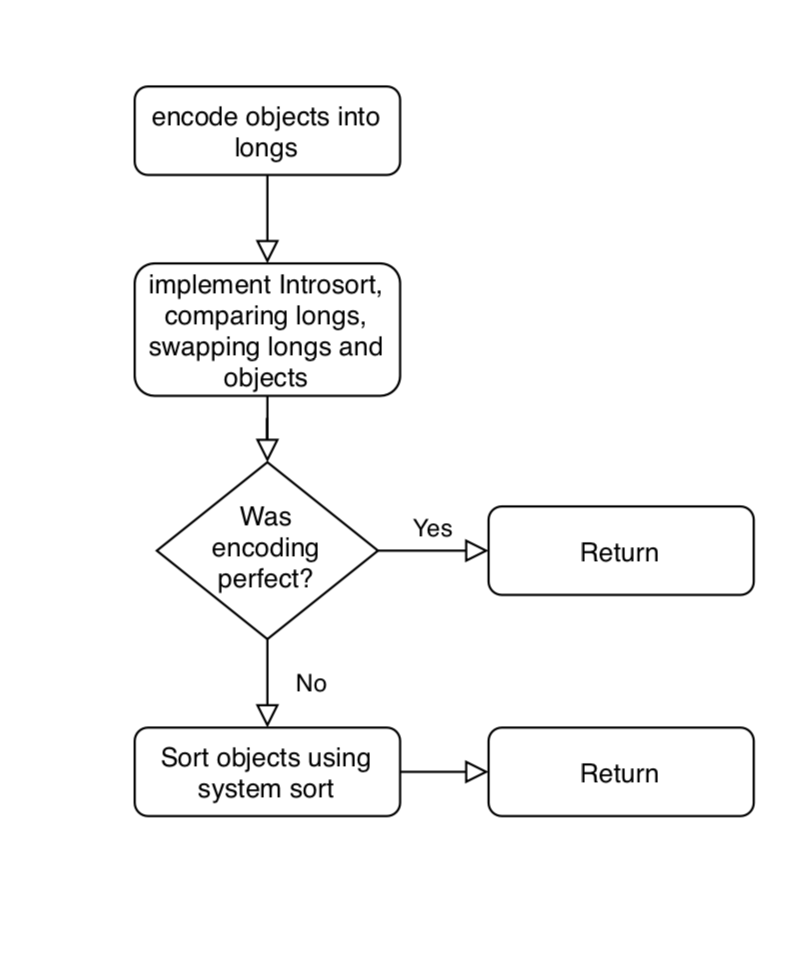
\includegraphics[trim=62 74 22 38, clip, width=0.39\linewidth]{HuskySortFlow.png}
\end{figure}
The strategy of HuskySort (see Flow ~\ref{Fig:HS}) is as follows,
assuming the dataset is presented as an array $xs$ of type $X$:


\begin{steps}
\item  
\renewcommand{\labelenumi}{\alph{enumi}}
    \begin{enumerate}
    \item Create a $long[]$ array (\emph{longs}) of the same size as $xs$;
    \item for each element $x$ of $xs$, set the corresponding element of \emph{longs} to $x.huskyCode()$.
    \end{enumerate}
\item {}Sort array \emph{longs} using quicksort (in practice, we have found that Introsort\cite{doi:10.1002} works well)
in such a way that when elements $i, j$ of \emph{longs} are exchanged, then elements $i, j$ of $xs$ are also exchanged;
\item {}Finally, when quicksort is finished and, if necessary,
we run Timsort on the array $xs$ to ensure that its elements are truly in order.
\end{steps}

For a worked example of a husky coding, see Algorithm ~\ref{alg:permitcoder}

\subsection{RadixHuskySort.}
\label{sec:radix}

Step 2 sorts the husky codes using Introsort, an $\textbf{O}(N log N)$ algorithm,
but the codes themselves are fixed-width 64-bit values,
and radix sort can sort $k$-bit keys in $\textbf{O}(N \cdot \frac{k}{b})$ time using $b$-bit digits —
linear in $N$ for any fixed digit width $b$.
Given that HuskySort's entire premise is to move work from the linearithmic phase to the linear phase,
this raises a natural question we had not previously addressed:
could step 2 itself be made linear? This section describes RadixHuskySort, which we built to answer it (Algorithm ~\ref{alg:the_alg5}).

Radix sort's linear-time advantage rests on a further assumption beyond fixed key width:
that a digit can be turned into an array index in $\textbf{O}(1)$ time,
so that counting and scattering never need to compare two digits directly.
A $b$-bit digit of a husky code satisfies this trivially —
it is extracted by a single shift and mask, and used directly as an index into a $2^b$-bucket counting array.
The original \textit{Comparable} type generally does not:
without first reducing it to such a code, radix sort applied directly to a \textit{String},
a \textit{Tuple}, or a case class would need some other way to decide which of $2^b$ buckets a given key belongs to,
and whenever the natural notion of a "digit" for such a type is not already a small, dense integer,
that decision falls back to \textit{equals} (and, for a hash-based bucket structure,
\textit{hashCode}) on the type itself — an $\textbf{O}(\text{size of the value})$ operation, not an $\textbf{O}(1)$ one.
Husky encoding is what removes this cost from every one of RadixHuskySort's $\frac{64}{b}$ digit passes,
not merely from the final comparison:
once the one-time $\textbf{O}(N)$ encoding step has run,
\textit{equals} and \textit{hashCode} on the original type are not called again until the optional cleanup pass.

A naive adaptation — swapping the object reference alongside each long at every exchange within every digit pass,
exactly as step 2's Introsort swaps at every partition exchange —
would incur $\textbf{O}(N)$ reference movements per digit pass, or $\textbf{O}(N \cdot \frac{64}{b})$ movements in total.
Since $\frac{64}{b}$ is typically much smaller than $log N$ at the sizes we tested,
this would still usually beat Introsort's swap cost,
but it needlessly reintroduces exactly the kind of payload-movement overhead this whole design exists to avoid,
and least-significant-digit (LSD) radix sort's per-pass counting-sort structure makes a better option available.

Instead, RadixHuskySort's step 2 carries only an $\textit{int[]}$ index array through the LSD digit passes,
alongside the (unmodified) long array;
each pass is a stable counting sort keyed on one $b$-bit digit of the (already-computed) husky code,
reordering the index array rather than the codes or the objects themselves.
Once all $\frac{64}{b}$ passes are complete, the index array holds the sorting permutation,
and a single $\textbf{O}(N)$ pass builds the final object array by reading $\textit{xs[index[i]]}$ for each $i$.
This confines all object-reference movement to one pass total, rather than one pass per digit.

Because LSD radix sort's per-digit counting sort treats keys as unsigned,
and husky codes are signed 64-bit values whenever the underlying domain can be negative (e.g., \textit{Integer},
\textit{Long}, or dates before a chosen epoch), each code is first transformed by $\textit{code} \oplus \textit{Long.MIN\_VALUE}$ —
flipping only the sign bit — before the digit passes,
which places negative codes before non-negative ones under unsigned digit comparison without disturbing relative order within either group;
the same transform is idempotent to reverse, so no separate un-flip step is needed once the permutation is built from the transformed codes.
Whether a given \textit{HuskyCoder} can actually produce negative codes is checked rather than assumed,
since several codings (e.g., Unicode strings) never do.

The digit width $b$ is a tunable parameter, trading off the number of passes ($\frac{64}{b}$)
against the size of the per-pass counting array ($2^b$ buckets, which must fit comfortably in cache for each pass to stay fast);
\S~\ref{sec:radix-results} reports how this trade-off plays out empirically across data types and array sizes.
Step 3 (the cleanup pass, run only if the coding is not provably \textit{perfect})
is unchanged regardless of which algorithm sorts the codes in step 2 —
radix sort is a drop-in replacement for that one step, not a change to the overall three-step strategy.

This parameterization also addresses a related limitation:
assuming 64-bit words throughout may not be appropriate for comparison on different key sizes.
Quicksort's asymptotic behaviour does not depend on key width at all —
an $\textbf{O}(N \log N)$ comparison sort costs the same whether the keys being compared are 32 bits or 128 bits wide,
since only the (fixed-cost) comparison itself touches the key's actual bits.
Radix sort, by contrast, makes the key width an explicit, first-class parameter:
a $k$-bit key simply takes $\frac{k}{b}$ passes instead of $\frac{64}{b}$, with no change to the algorithm itself.
So while nothing about the discussion above depends on 64-bit words specifically,
the RadixHuskySort generalizes to other key widths more directly than a comparison-based sort does —
if a future encoding needed, say, 128 bits to capture more of an object's structure,
the same radix sort would apply unchanged, merely with twice as many passes.

Radix sort applied to strings specifically has its own substantial, and older, literature,
distinct from the general fixed-width-key radix sort described above.
Three-way radix quicksort (also called multikey quicksort) and MSD (most-significant-digit)
radix sort for strings were both popularized by Bentley and Sedgewick's classic treatment\cite{314161.314321},
and burstsort\cite{1064546.1180622} improves cache behaviour further by building a small trie to bucket strings before sorting.
These string-specialized algorithms sort variable-length strings directly, character by character, without a separate fixed-width encoding step.
RadixHuskySort's contribution is different in kind, not degree:
it is not a string-sorting algorithm, but a general mechanism applicable to any \textit{Comparable} type
with a 64-bit husky encoding (strings among them),
at the cost of the encoding's own fixed capture window (\S~\ref{sec:pcrit} above)
and a fallback cleanup pass whenever that encoding is imperfect.

That framing carries a consequence which Table ~\ref{tab:RadixImprovements} bears out,
and which we state rather than leave to be noticed:
the string rows of that table are its most variable by a wide margin.
They span from 3.4x down to 1.6x, nearly the whole of its range below dates,
where every other row falls between 2.1x and 3.6x.
Three factors account for the spread, and they compose.
The advantage grows with the cost of the type's native comparison, since that is what the encoding replaces;
it grows with the perfection of the encoding, since an imperfect one is paid for by the cleanup pass;
and it shrinks in the presence of algorithms specialised to the type.
Dates are the favourable extreme on all three counts --- a provably perfect coding, no cleanup pass at all,
and no specialised competitor --- and yield the largest margin in the table at 5.9x.
The string rows show those same three factors varying \emph{within} a single data type,
which is the more instructive demonstration.
Chinese words are favourable on the first two counts --- an expensive Unicode comparison,
captured well enough by the encoding --- and sit fourth of eleven, above all but three of the non-string rows.
Chinese personal names are unfavourable on the second: the comparison is more expensive still,
a table lookup per character, but the pinyin coding captures far less of the key than the Unicode
coding does, so ties are common and the cleanup pass does real work rather than none
(\S~\ref{sec:chinese-coders} accounts for the difference).
The more expensive comparison is paired with the weaker encoding, and this is the weakest result we report.
English words are unremarkable on the first two counts and distinctive on the third,
being the one case in this paper with a mature specialised literature ranged against it.

Strings are unfavourable on the third count in a way no other type in this paper is.
Half a century of specialised string sorting exists,
and a general mechanism should not be expected to beat it on its own ground.
We compared RadixHuskySort against both of the classic string sorts named above,
under JMH, on English and Chinese text, in code-point order so that every sort compared
performs the same task.
Both baselines are our own implementations,
each tuned so that its fallback below the partitioning cutoff allocates nothing
and compares from the depth the partitioning has already established.
Against three-way radix quicksort RadixHuskySort is faster at every size tested,
by 1.3--2.4x on English words and 3.1--4.0x on Chinese words,
with non-overlapping 99.9\% confidence intervals throughout.
Against MSD radix sort the result goes the other way at scale, though not by much:
on English text the two are indistinguishable at $N=32{,}000$,
and MSD is faster by 1.20x at $N=200{,}000$ and by 1.06x at $N=1{,}000{,}000$.
The advantage at $N=200{,}000$ is the robust one.
At $N=1{,}000{,}000$ three runs on the machine of record give 1.00x, 1.05x and 1.06x,
so at the largest size we measure the two algorithms are level to within the spread between runs,
and the direction should be read from the middle size rather than the largest.
We give this result because it locates the boundary rather than obscuring it.
MSD earns it on a corpus that suits it and within limits that are its own:
our implementation indexes an alphabet of 256 characters beyond ASCII,
which English text fits and neither Chinese corpus does,
and it offers no pinyin ordering,
so there is no MSD row for either Chinese corpus.
RadixHuskySort reaches every corpus in this paper through one encoding,
with no per-alphabet provision and no per-type implementation.
That is the claim being made, and the English result bounds it without contradicting it.
A direct empirical comparison against burstsort remains future work;
it is a trie-based, cache-conscious algorithm designed to beat both baselines used here on exactly this workload,
and we have not implemented it.

Code-point order is not a meaningful comparison for Chinese personal names specifically —
it is simply the wrong order for that use case, not merely a different one.
Leaving the word corpus in that order is deliberate: a directory of people has one conventional
ordering and it is by pinyin, where a word list has several --- by radical, stroke count, pinyin or
frequency, according to purpose --- so no single ordering is the right one to hold it to,
and code-point order keeps that row comparable with the English one.
A fair comparison for the names requires a pinyin-aware MultikeyQuicksort.
We extended it with the same syllable-then-tone character key the pinyin encoding of \S~\ref{sec:radix} already uses,
restricted the comparison to the three pinyin-aware sorters, and re-ran it.
RHSort is faster than the repaired multikey quicksort by 1.57x, 1.83x and 2.09x at $N = 32{,}000$,
$200{,}000$ and $1{,}000{,}000$, and QuickHuskySort by 1.33x, 1.49x and 1.27x.
Two independent runs on the machine of record agree to within two hundredths of those multipliers.
Note that the RHSort margin grows with $N$ while QuickHuskySort's does not:
the linear second phase keeps paying as the array grows where a linearithmic one cannot,
which is the same pattern the natural-order corpora show and the clearest form in which this corpus
shows it.

\begin{algorithm2e}
\KwIn{\it{xs} as an array of object X which extends Comparable<X>}
\KwIn{\it{b} as the number of bits per digit}
 coding = huskyCoder.huskyEncode(xs)\;
 longs = coding.longs\;
 index = radixSortIndices(longs, b)\;
 ys = permute(xs, index)\;
 \If{coding.perfect}{return ys\;}
 Arrays.sort(ys)\;
 \caption{RadixHuskySort.sort}
 \label{alg:the_alg5}
\end{algorithm2e}

\begin{algorithm2e}
\KwIn{\it{longs} as an array of long}
\KwIn{\it{b} as the number of bits per digit}
\KwOut{\it{index}, a permutation of $0, \ldots, \textit{longs.length} - 1$ such that
  \textit{longs[index[$\cdot$]]} is sorted}
 biased[i] = longs[i] {\bf XOR} Long.MIN\_VALUE, for each i\;
 index = [0, 1, \ldots, longs.length - 1]\;
 \For{digit = 0 \KwTo (64 / b) - 1}{
 index = stableCountingSortPass(biased, index, digit, b)\;
 }
 \caption{radixSortIndices (LSD, deferred permutation)}
 \label{alg:the_alg6}
\end{algorithm2e}

\subsection{Discussion of Husky Encoding.}

Step 1b requires the definition of a 64-bit hash function (huskyCode) whose properties are as follows:
(refer to Algorithm ~\ref{alg:the_alg2})
\begin{itemize}
                        \item {}If $x = y$, then $x.huskyCode() = y.huskyCode()$;
                        \item {}If $x > y$, then: 
                            \begin{itemize}
                            \item{} either $x.huskyCode() <= y.huskyCode()$ (with probability $p$)
                            \item{} or $x.huskyCode() > y.huskyCode()$ (with probability $1-p$);
                            
                            \end{itemize}
                        
                        \end{itemize}


We interpret this rule as follows:
if $x$ and $y$ are the same ($x.equals(y)$ in Java), their huskyCode should be the same.
If $x > y$, we normally expect that $x.huskyCode() > y.huskyCode()$, i.e., the sort on the husky-coded longs will not invert $x$ and $y$.
However, when $x > y$ while $x.huskyCode() < y.huskyCode()$, then an inversion will be introduced.
And, when $x > y$ and $x.huskyCode() = y.huskyCode()$, then an inversion \emph{may} be introduced because quick-sort is not stable.\cite{6115063}

For a successful encoding, the value of $p$, the probability of a potential inversion, should be less than some critical probability, $p_{crit}$.
Leaving a more detailed discussion of $p_{crit}$ until later, we note that, for some domains of $X$, we can definitely assert that $p = 0$.
We refer to this as a “perfect” encoding.
In such a case, we can skip step 3 of the algorithm because, when $p = 0$, there will be no inversions remaining after quick-sorting according to the huskyCodes.
An example of such a domain is date-time values with a resolution of one nano-second over a period of 128 years.
For strings of English case-independent letters (no punctuation or numbers), i.e., 5-bit ASCII, words of 12 (or fewer) characters in length can also be coded uniquely.
For case-dependent strings (6-bit ASCII), we can encode perfectly if the lengths are all 10 characters or less.
In step 3, it might be acceptable to use insertion sort instead of Timsort.
In any event, assuming that the huskyCode is as accurate as required, then there will be very few inversions (elements out of place) remaining after the quicksort phase.
This implies that the second sort can be performed in very close to linear time.
The results have been very satisfactory.
For example, taking an array of 1,000,000 English words drawn randomly from a corpus of 275,333\cite{GOLDHAHN12.327},
QuickHuskySort sorts in 698 ms against the system sort's 1,121 ms, a factor of 1.61
(for the full data, please refer to table ~\ref{tab:HS_BM}).






\subsection{Discussion of \texorpdfstring{$p_{crit}$}{p\_crit}.}
\label{sec:pcrit}
When $p > 0$, there is a finite probability of any pair of elements remaining inverted after the first sorting pass.
For an array of N randomly ordered elements, the average number of inversions before sorting is $X = N (N -1 ) / 4$.
The number of inversions remaining after the first pass is simply $p X$.
And, for Timsort or insertion sort, the time to re-sort the array will be $t = k (N + p X)$ where $k$ is some system-dependent constant.
The total time to sort the array is made up of these three time-consuming steps where $k_1, k_2, k_3$ are system- and algorithm-dependent constants:

\begin{steps}
 \item{} $T_1$ is the time to encode the elements:
\[T_1 = k_1 N\]
\item{}  $T_2$ is the (average) time to quick-sort the huskyCode array while also swapping the element array itself:
\[T_2 = 2 k_2 N ln N\]
\item{}  $T_3$  is the time to Timsort the element array (only required if $p>0$):
 \[T_3 = k_3 (N + p X)\]
\end{steps}
Provided that the total time $T = T_1 + T_2 + T_3$ is less than the time required to use Timsort on the original element array, we have a win.
This same three-step decomposition ($T_1$/$T_2$/$T_3$, i.e., encode/sort/cleanup) is revisited in \S~\ref{sec:analysis}
in more concrete terms —
counting array accesses directly rather than folding everything into abstract system-dependent constants $k_1, k_2, k_3$ —
and extended there to cover RadixHuskySort (\S~\ref{sec:radix}) as a fourth alternative for the $T_2$ step.
The actual values of $p_{crit}$ are very much dependent on the machine running the sort.
We have not calculated a typical value for $p_{crit}$ but, even for the worst-case:
Chinese characters using UTF8 encoding, we still find very significant gains, reported later in Table ~\ref{tab:HS_BM}.

Of the three terms, $T_3$ can be isolated experimentally.
Two benchmarks over the same two hundred thousand municipal records (\S~\ref{sec:radix-results})
differ only in which coder they are given.
Both compute identical codes; one coder declares itself perfect, so the sort skips step 3,
while the other leaves that declaration at its default and the pass runs.
The encoding for these records is perfect, so the pass that runs has provably nothing to correct.

Its cost is predictable in advance.
Timsort over a fully ascending array detects a single run and stops,
performing $N-1$ comparisons and no moves,
so $T_3$ at $p = 0$ is exactly $N-1$ invocations of the element's own comparator ---
here assessor's block, then lot, then filing date,
which is precisely the comparison the husky encoding was introduced to avoid.
The cleanup pass reintroduces one full composite comparison per element,
having just removed it from all $\textbf{O}(N \log N)$ of them.

That comparison costs 16.1\,ns at $N = 32{,}000$, 60.3\,ns at $N = 100{,}000$ and 74.2\,ns at
$N = 198{,}900$ --- 7.3\%, 17.2\% and 17.3\% of the running time of the sort that contains it ---
with non-overlapping 99.9\% confidence intervals throughout.
Three further runs, one of them on different hardware, agree on the shape at different levels;
across all four the pass costs between a sixteenth and a quarter of the total,
and between a sixth and a quarter at the two larger sizes.
The percentages are the less stable figures, being ratios of two quantities that both move.
The shape is a threshold rather than a trend --- a rise by a factor of roughly three to four between the first two sizes,
then a levelling off --- and it falls where the records stop fitting in cache.
That last reading is inference, but the magnitudes support it:
the system sort compares these same records some 3.5 million times in 151\,ms, or 43\,ns each,
so the cleanup pass at 74\,ns costs nearly twice as much per comparison using the same comparator.
Step 2 permutes references without moving the records,
so a scan sequential in the array is close to random in the heap.

Whether this share must shrink as $N$ grows --- the pass being linear where the sort containing it is
linearithmic --- is a fair question, and \S~\ref{sec:cleanup-scaling} answers it.

Two conclusions follow.
First, $k_3$ is not a constant: it varies more than fourfold across three sizes on one machine,
so no single $p_{crit}$ can be quoted even for one type on one machine.
Second, an encoding which can be declared perfect avoids a cost of up to a quarter of total running
time, where one which cannot must repay it before correcting a single genuine inversion.

\subsection{Why husky coding works.}
\label{sec:why-husky}

The rationale is set out in full by Hillyard et al.\cite{huskysort2020}; we restate only what the rest of
this paper depends on.
A 64-bit word holds enough of most keys to place elements close to their final order, and comparing two
longs costs far less than following two object references and running a type-specific
\textit{compareTo} --- so the encoding trades one $\textbf{O}(N)$ pass for cheaper comparisons throughout
the $\textbf{O}(N \log N)$ one.
The code need not be perfect, only good: whatever inversions it leaves are the cleanup pass's problem, and
\S~\ref{sec:pcrit} measures what they cost.

Perfection has a precise limit for strings.
Packing four 16-bit characters fills the word (Table ~\ref{tab:EncodingConstants} gives the constants for
both string codings), but the packed result is then shifted right by one bit, because any string whose
first character is \texttt{0x8000} or above --- common among CJK characters --- would otherwise set the
sign bit and encode as a negative \textit{long}, corrupting numeric comparison.
The shift costs the least significant bit of a true fourth character; for three characters or fewer that
bit is padding, which is why the Unicode coding is declared \textit{perfect} up to three characters and
not four.

Whether a coding was in fact perfect is known before the cleanup pass runs: a constant-time lookup for
non-sequence types, and for strings a scan that stops at the first string too long to encode perfectly.
Where it was perfect, no inversions remain and the pass is skipped altogether.


\begin{algorithm2e}
\KwIn{\it{xs} as an array of object X}
\KwOut{A new \it{Coding} object}
 result = new long[xs.length]\;
 \For{i = 0 to xs.length}{
 result[i] = huskyEncode(xs[i])\;
 }
 return new Coding(result, perfect())\;
 \caption{huskyEncode}
 \label{alg:the_alg2}
\end{algorithm2e}


\begin{algorithm2e}
\KwIn{\it{permit}, with fields \it{block}, \it{lot}, \it{filedDate}\;}
\KwOut{a 60-bit code, order-preserving for \it{permit.compareTo}}
 \tcp{fields most-significant first, in compareTo order}
 r = encodeString(block, 5, 5, BLOCK\_ALPHABET)\;
 r = r $\ll$ 24 $|$ encodeString(lot, 4, 6, LOT\_ALPHABET)\;
 \Return r $\ll$ 11 $|$ daysSinceEpoch(filedDate)\;
 \BlankLine
 \tcp{codeOf(x, alphabet), used by encodeString for each symbol}
 \eIf{alphabet contains x}{
   \Return 1 + index of x\tcp*{0 is left for padding}
 }{
   \Return count of symbols $<$ x\tcp*{weaken, never invert}
 }
 \caption{A composite husky coder: \textit{PermitCoder}. \textit{encodeString} packs \textit{width}
   symbols of \textit{bits} each, right-padding with zero.}
 \label{alg:permitcoder}
\end{algorithm2e}

\section{Implementation.}

%% ANONYMISATION: the real URL names its owner, so it is guarded with the author block. See
%% "0i. The repository link" in Paper edits pending.md -- the Anonymous GitHub mirror is task 2
%% on Sai Vineeth's list; when its URL exists, substitute it for the placeholder below and the
%% review copy can cite the code directly.
\ifanonymous
  The implementation is available in an anonymised repository, linked from the submission site.
\else
  The implementation is available at \url{https://github.com/rchillyard/HuskySort}.
\fi

\subsection{System Environment.}

Three machines appear in this paper, and \S~\ref{sec:environments} specifies all three.
Machine A ran the JDK 1.8.0\_152 comparison-sort benchmarks of \S~\ref{sec:analysis},
the choice of cleanup sort among them (\S~\ref{sec:cleanup-choice});
machine B, on different hardware and two JVM generations later, ran the radix-sort and JMH development work.
Machine C is the machine of record: an independently administered cloud instance, confirmed idle before
each run, and the source of every figure quoted in this paper.
It is ARM-based like machine B but differs from it in core design, vendor, core count and operating system.

Reporting all three lets a reader check directly whether the qualitative finding generalizes across
machines and JVM versions rather than being an artifact of one environment.
It does: QuickHuskySort, and now RHSort, beat the system sort on all three,
which differ in vendor, instruction set, core design and JVM generation.



\begin{table}
  \caption{String-encoding constants}
  \label{tab:EncodingConstants}
  \begin{tabular}{lll}
    \toprule
    Constant & Unicode & ASCII \\
    \midrule
    Bit width per character & 16 & 7 \\
    Max length (64 / bit width) & 4 & 9 \\
    Mask & \texttt{0xFFFF} & \texttt{0x7F} \\
    \bottomrule
  \end{tabular}
\end{table}

\section{Test Case and Analysis.}

\subsection{Data Source.}
\label{sec:data-source}
The sources for the Strings (English and  Chinese) are retrieved from Leipzig Corpora Collection\cite{GOLDHAHN12.327}.
Chinese personal names, used for the pinyin-order comparisons of \S~\ref{sec:radix-results}, are a separate corpus\cite{wainshine2020chinesenames}.
Every other dataset in this paper is generated: pseudo-random numbers, dates and tuples.
The building-permit records of \S~\ref{sec:radix-results} are not.
They are 198,900 permits filed between January 2013 and February 2018, taken from San Francisco's published
record\cite{sf-building-permits} and ordered by a composite key of assessor's block, lot and filing
date; they are included because their distribution is the city's rather than ours.
Only those three columns are retained, and the data is used under the Open Data Commons Database
Contents License.

In each case, we take data from the appropriate \emph{sentences.txt} file and break it up into strings as shown in Listing~\ref{lst:DS}.


\begin{lstlisting}[caption={Data Source},label={lst:DS},language=Java]
private static String[] getLeipzigWordsFromResource(final String resource) {
    return getWords(resource, HuskySortBenchmark::getLeipzigWords);
}
private static List<String> getLeipzigWords(final String line) {
    return HuskySortBenchmarkHelper.splitLineIntoStrings(line, REGEX_LEIPZIG, REGEX_STRINGSPLITTER);
}
final static Pattern REGEX_LEIPZIG = Pattern.compile("[~\\t]*\\t(([\\s\\p{Punct}\\uFF0C]*\\p{L}+)*)");
public static final Pattern REGEX_STRINGSPLITTER = Pattern.compile("[\\s\\p{Punct}\\uFF0C]");


static List<String> splitLineIntoStrings(final String line, final Pattern lineMatcher, final Pattern stringsplitter) {
    final Matcher matcher = lineMatcher.matcher(line);
    if (matcher.find()) return Arrays.asList(stringsplitter.split(matcher.group(1)));
    else return new ArrayList<>();
}

static String[] getWords(final String resource, final Function<String, List<String>> stringListFunction) {
    try {
        File file = new File(getPathname(resource, DutchHuskySort.class));
        return getWordArray(file, stringListFunction, 2);
    } catch (FileNotFoundException e) {
        logger.warn("Cannot find resource: "+resource, e);
        return new String[0];
    }
}
    } catch (final Exception e) {
        throw new RuntimeException(e);
    }
}


\end{lstlisting}

\subsection{Analysis.}
\label{sec:analysis}
Let’s try to do an analysis of QuickHuskySort's performance.
This expands on the $T_1$/$T_2$/$T_3$ decomposition introduced in \S~\ref{sec:pcrit} above,
replacing its abstract time constants with concrete array-access counts,
and extending it to cover RHSort (\S~\ref{sec:radix}) as an alternative to quicksort for the $T_2$ step.
The first thing to note is that, like merge sort, QuickHuskySort requires $\textbf{O}(N)$ extra space.
This is because, in addition to the array of object references, we must have an equal-length array of longs (the huskyCode values).

Secondly, QuickHuskySort is not stable unless using the merge sort variation.
The derivation of the two comparison figures is a counting argument rather than a measurement, and it
rests on one coefficient we estimated rather than measured; it is set out in \S~\ref{sec:qhs-analysis}.

Encoding's cost has not simply been assumed:
we timed the encoding phase in isolation,
separately from the sort that follows it, to confirm it directly.
At $N = 1{,}000{,}000$, encoding takes 67.7ms for English words (9.7\% of QuickHuskySort's 697.9ms total,
24.8\% of RHSort's 272.7ms) and 211.1ms for Chinese names encoded via pinyin (16.9\% of QuickHuskySort's
1252.7ms, 27.8\% of RHSort's 760.9ms) — confirming that encoding cost, while real and non-negligible,
especially for the more elaborate pinyin encoding, remains a minority of total time in every case measured,
consistent with the linear-and-subordinate role it is assumed to play above.
Encoding's share of the total is larger for RadixHuskySort than for QuickHuskySort in both cases,
simply because RHSort's own contribution to the total is smaller —
as the sort phase gets cheaper,
whatever cost remains in the encoding phase necessarily becomes a proportionally larger slice of what is left,
which suggests encoding cost (particularly for pinyin)
is the more promising target for further optimization now that the sort phase itself is no longer the dominant cost.
The consequence of this is that, as expected,
the linear phase of QuickHuskySort is relatively high for small $N$ but that is soon swamped by the saving of comparisons in the linearithmic phase.
The break-even point is actually a very small value of $N$:
four.
As $N$ increases, we expect the advantage of QuickHuskySort to increase further.
This is generally borne out by the benchmarks.
Please refer to table ~\ref{tab:Comparison}.

The same style of analysis extends naturally to RadixHuskySort (\S~\ref{sec:radix}).
Each of its $\frac{64}{b}$ digit passes touches every element a small constant number of times,
$c$, to bucket it and to record its new position in the (deferred) index array —
with no partitioning or pivot-comparison overhead, and critically, no logarithmic term at all.
Taking $c = 4$ (the same per-exchange cost used for QuickHuskySort's swaps above),
adding the final $\textbf{O}(N)$ pass that applies the resulting permutation to the object array (2 array accesses per element),
and the same encoding cost ($(k+1)N$) and cleanup-pass cost ($(2 + j + 4)pN$,
unaffected by which algorithm sorts the codes in step 2), the total array accesses for RadixHuskySort ($A_r$) come to:
\[A_r = \left(4 \cdot \frac{64}{b} + 2 + k + 1\right) N + (2 + j + 4)pN\]
Using the same illustrative constants as above ($j = 4$, $k = 7$, $p = 0.1$)
and $b = 16$ (four digit passes, near the middle of the digit-width plateau found empirically —
see \S~\ref{sec:radix-results}):
\[A_r = 27 N\]
Table ~\ref{tab:Comparison} extends the earlier comparison with this term.
At $N = 1{,}000{,}000$, $A_r \approx 27{,}000{,}000$ against $A_h \approx 101{,}000{,}000$ and $A_m \approx 161{,}000{,}000$ —
a predicted advantage of roughly 3.7x over QuickHuskySort,
consistent with the 2-4x speedups actually measured (\S~\ref{sec:radix-results}).
The model does predict one caveat:
equating $A_r$ and $A_h$ gives a theoretical break-even around $N \approx 17$,
somewhat higher than QuickHuskySort's own break-even against merge sort ($N = 4$,
above) — because RHSort's per-pass cost has no logarithmic term to shrink relative to at very small $N$.
This crossover is far below every array size actually tested, so it has no practical effect on the results reported here,
but it is worth stating rather than leaving the model looking like radix wins unconditionally at every $N$.
 \begin{table*}
  \caption{Theoretical comparisons (array accesses, dimensionless counts)}
  \label{tab:Comparison}
  \begin{tabular}{rrrrr}
    \toprule
    N  &  N ln N & merge sort & QuickHuskySort & RHSort \\
    \midrule
     4 & 6 & 72 & 72 & 108 \\
     1,000 & 6,908 & 81,439 & 55,075 & 27,000 \\
     1,000,000 & 13,815,511 & 160,878,371 & 101,149,455 & 27,000,000 \\
     1,000,000,000 & 20,723,265,837 & 240,317,557,125 & 147,224,183,132 & 27,000,000,000 \\

    \bottomrule
  \end{tabular}
\end{table*}

Since the final pass of HuskySort will be cleaning up a relatively small number of inversions, does it
matter whether we use insertion sort or Timsort?
Below about 50,000 Strings it makes barely any difference, and insertion sort is sometimes faster;
beyond that Timsort wins out, by a factor of four and a half at $N = 4{,}000{,}000$.
That measurement, and the choice it settles, are in \S~\ref{sec:cleanup-choice}.


\section{Results and Observations.}
\subsection{Benchmarks.}

Table ~\ref{tab:HS_BM} reports absolute sort times for every data type and corpus.
The two radix columns bracket the digit-width plateau of \S~\ref{sec:radix-results}.
Dual-pivot quicksort and a from-scratch quicksort were measured too; they bear on QuickHuskySort
rather than on RHSort, so they are in \S~\ref{sec:comparison-baselines}.

\begin{table*}
  \caption{Sort times by data type (JMH, ms, mean $\pm$ 99.9\% CI). Numeric types at $N=500{,}000$.
    For Chinese names the system-sort column is a system sort performing the same pinyin ordering;
    code-point order is a different and much cheaper task (\S~\ref{sec:radix-results}).}
  \label{tab:HS_BM}
  \begin{tabular}{llllll}
    \toprule
    Data type & N & System sort & QuickHuskySort & RHSort/8 & RHSort/16 \\
    \midrule
    Integer & 500,000 & 121.2$\pm$0.6 & 89.7$\pm$3.5 & 31.2$\pm$0.5 & 25.2$\pm$0.2 \\
    Double & 500,000 & 141.7$\pm$1.3 & 97.8$\pm$3.6 & 34.0$\pm$0.5 & 31.0$\pm$0.3 \\
    Long & 500,000 & 135.8$\pm$1.2 & 97.7$\pm$1.0 & 30.2$\pm$0.2 & 28.6$\pm$0.3 \\
    BigInteger & 500,000 & 208.4$\pm$1.7 & 152.3$\pm$1.7 & 56.9$\pm$0.3 & 54.1$\pm$0.2 \\
    BigDecimal & 500,000 & 262.2$\pm$1.6 & 144.1$\pm$2.1 & 54.1$\pm$0.3 & 52.5$\pm$0.3 \\
    English words & 32,000 & 13.69$\pm$0.19 & 9.72$\pm$0.12 & 4.63$\pm$0.16 & 4.18$\pm$0.16 \\
    & 200,000 & 141.39$\pm$2.59 & 94.74$\pm$2.44 & 55.01$\pm$2.20 & 50.27$\pm$2.51 \\
    & 1,000,000 & 1120.87$\pm$14.43 & 697.88$\pm$16.15 & 355.26$\pm$24.71 & 272.74$\pm$6.46 \\
    Chinese words & 32,000 & 9.78$\pm$0.08 & 5.00$\pm$0.04 & 2.10$\pm$0.03 & 1.89$\pm$0.02 \\
    (code-point order) & 200,000 & 71.34$\pm$0.63 & 30.90$\pm$0.13 & 13.49$\pm$0.15 & 10.85$\pm$0.10 \\
    & 1,000,000 & 447.12$\pm$2.28 & 219.80$\pm$1.99 & 83.25$\pm$2.31 & 65.46$\pm$1.47 \\
    Chinese names & 32,000 & 69.1$\pm$1.4 & 26.6$\pm$0.3 & 24.1$\pm$0.2 & 23.1$\pm$0.3 \\
    (pinyin order) & 200,000 & 526.2$\pm$9.5 & 187.2$\pm$1.0 & 157.0$\pm$1.3 & 154.9$\pm$1.2 \\
    & 1,000,000 & 3112.9$\pm$68.0 & 1252.7$\pm$6.4 & 775.7$\pm$4.2 & 767.2$\pm$14.0 \\
    Tuples & 20,000 & 3.72$\pm$0.01 & 2.79$\pm$0.02 & --- & 1.30$\pm$0.01 \\
    & 100,000 & 23.24$\pm$0.19 & 17.65$\pm$0.16 & --- & 6.82$\pm$0.05 \\
    & 500,000 & 209.53$\pm$7.98 & 142.61$\pm$1.83 & --- & 57.98$\pm$0.76 \\
    \bottomrule
  \end{tabular}
\end{table*}

\subsection{Summary.}
\label{sec:summary}
HuskySort’s target application is the sorting of randomly ordered arrays of objects on the JVM (Java Virtual Machine).
Let’s eliminate the non-use-cases first:
\begin{itemize}
\item {}Partially-ordered arrays:
that’s to say, arrays with only a linear number of inversions as would be the case when adding a relatively small number of records to a large existing index.
For such use cases, Timsort (the Java system sort for objects) would be more suitable.

\item {}Arrays of primitives:
in Java, a clear distinction exists between primitive types (char, byte, short, int, float, long, double) and objects.
Dual-pivot quicksort (the Java system sort for primitives) is already the fastest algorithm for sorting such types.
\end{itemize}
Thus, HuskySort is best for any object array where there’s no expectation of partial ordering.
Typical improvements over Timsort can be read directly off Table ~\ref{tab:HS_BM} above, which gives
absolute times with 99.9\% confidence intervals rather than summary ranges:
1.4--1.8x across the five numeric types at $N=500{,}000$,
1.4--1.6x on English words,
2.0--2.3x on Chinese words,
and 1.3--1.5x on tuples.
Note that the English margin \emph{widens} with array size rather than decaying,
from 1.41x at $N=32{,}000$ to 1.61x at $N=1{,}000{,}000$.

\subsection{Radix Sort Results.}
\label{sec:radix-results}

We benchmarked every data type and corpus covered above using RadixHuskySort (\S~\ref{sec:radix})
in place of Introsort for step 2, using JMH (the Java Microbenchmark Harness, with proper fork isolation and warmup) on JDK 21.

Table ~\ref{tab:RadixImprovements} reports RHSort's advantage over QuickHuskySort as a direct multiplier —
e.g., \textbf{2.9x} means radix took roughly a third as long —
rather than as a percentage, since a percentage figure close to or above 100\% becomes ambiguous about exactly which quantity it is a percentage \emph{of}.

\begin{table*}
  \caption{RHSort's advantage over QuickHuskySort, as a direct multiplier}
  \label{tab:RadixImprovements}
  \begin{tabular}{cll}
    \toprule
    Data Type & N & Advantage over QuickHuskySort \\
    \midrule
    \texttt{Dates} & 20,000 & 5.9x \\
    \texttt{Long} & 500,000 & 3.6x \\
    \texttt{Integer} & 500,000 & 3.6x \\
    \texttt{Strings of Chinese words (code-point order)} & 1,000,000 & 3.4x \\
    \texttt{Double} & 500,000 & 3.2x \\
    \texttt{BigInteger} & 500,000 & 2.8x \\
    \texttt{BigDecimal} & 500,000 & 2.8x \\
    \texttt{Strings of English words} & 1,000,000 & 2.6x \\
    \texttt{Tuples} & 500,000 & 2.5x \\
    \texttt{Building permits (composite key)} & 198,900 & 2.1x \\
    \texttt{Strings of Chinese names (pinyin order)} & 1,000,000 & 1.6x \\
    \bottomrule
  \end{tabular}
\end{table*}

This is worth confronting directly, since a reader might reasonably ask whether either advantage erodes
as $N$ grows: a constant-factor saving on a linearithmic sort could be swamped at scale.
Neither does.
QuickHuskySort's margin over the system sort on English text \emph{widens} with size,
from 1.41x at $N=32{,}000$ to 1.49x and then 1.61x (Table ~\ref{tab:HS_BM}),
and holds roughly constant on both Chinese corpora.
Radix sort's advantage over QuickHuskySort likewise does not shrink with $N$:
at every size and data type in Table ~\ref{tab:RadixImprovements}, the margin is 1.5x or greater,
consistent with the theoretical model of \S~\ref{sec:radix} predicting no logarithmic term at all,
so there is no analogous reason to expect the advantage to erode as $N$ grows further.
The spread across that table is itself informative, and follows the three factors of \S~\ref{sec:radix}.
Chinese names sorted by pinyin order are the smallest margin measured (1.6x),
because both QuickHuskySort and RadixHuskySort must pay the same cleanup pass for a coding
that two or three characters of recurring syllables leave badly imperfect.
Dates show the largest margin (5.9x) because that coding is provably perfect and never needs a cleanup pass at all,
letting RHSort's linear-time advantage show through with nothing else in the way.
The two lie at opposite ends of the same axis: what separates them is not the data type but the perfection of the encoding.

The building permits row is the only one in that table not measured on data we generated:
198,900 real municipal records ordered by a composite key of three fields (\S~\ref{sec:data-source}).
At 2.1x it is tenth of eleven, which is the point worth making about it --- it is not our largest
margin, but it is our largest on data whose distribution we did not choose.
\S~\ref{sec:permits} gives the case study, and \S~\ref{sec:composite-future} what a general
composite encoder would have to provide, that one having been written by hand.

The measurements were reproduced qualitatively on machines A and B of \S~\ref{sec:environments},
which differ from the machine of record and from each other in vendor, instruction set, core design and
JVM generation.
We quote no figures from them, since mixing environments within a comparison would rob it of meaning,
but every ordering reported here holds on all three.

\subsection{Parallel Radix Sort.}
\label{sec:parallel-radix}

Radix sort's digit passes are natural candidates for parallelization (\S~\ref{sec:radix} above).
We implemented and benchmarked a parallel variant:
each pass is split into a configurable number of contiguous chunks, one per worker thread.
Every chunk first computes its own local per-bucket histogram independently, with no synchronization required;
a short sequential step then combines those histograms into an exact starting offset, in the output array,
for every (chunk, bucket) pair — preserving the stability that step 3's cleanup pass, when needed, relies on,
since a chunk's elements always land after all lower-numbered chunks' elements sharing the same bucket;
finally, every chunk scatters its own elements into the output arrays independently,
using only its own precomputed offsets, so no two chunks ever write to the same location.

An initial implementation dispatched the two phases above to a thread pool separately on every pass.
Measurement showed this repeated dispatch itself contributing a real, non-trivial share of the total cost,
particularly at more moderate array sizes.
The overhead was substantially reduced by starting the worker threads once per sort,
rather than once per phase per pass:
each thread runs its own loop over every pass, and the two phases synchronize via reused barriers whose associated actions —
code that runs exactly once per synchronization point, in whichever thread arrives last —
perform the histogram-combine and buffer-swap steps.
Table ~\ref{tab:ParallelRadix} reports the result (\textit{Long[]}, 11-bit digits, milliseconds, mean $\pm$ 99.9\% CI).

\begin{table*}
  \caption{Parallel RHSort:
serial vs. 1, 2, 4, and 8 worker threads}
  \label{tab:ParallelRadix}
  \begin{tabular}{cccccc}
    \toprule
    N & Serial & 1 thread & 2 threads & 4 threads & 8 threads \\
    \midrule
    2,000,000 & 172.0$\pm$5.7 & 165.2$\pm$2.2 & 140.3$\pm$2.0 & 118.5$\pm$2.4 & 109.3$\pm$1.8 \\
    10,000,000 & 935.2$\pm$36.9 & 884.5$\pm$21.6 & 731.6$\pm$19.9 & 687.9$\pm$22.1 & 645.3$\pm$20.9 \\
    \bottomrule
  \end{tabular}
\end{table*}

Isolating parallelism itself, that's to say comparing 1 thread against 4, both paying identical thread-coordination overhead,
gives a statistically resolved speedup at both sizes: 1.39x at $N=2{,}000{,}000$ and 1.29x at $N=10{,}000{,}000$,
with non-overlapping confidence intervals in both cases.
Against the serial implementation the improvement is resolved at both sizes too,
172.0ms to 118.5ms at $N=2{,}000{,}000$ and 935.2ms to 687.9ms at $N=10{,}000{,}000$.
Unlike on the eight-core machine of an earlier draft, scaling does not stop at four threads:
on sixteen uniform cores, eight threads beats four at both sizes with intervals that do not overlap,
reaching 1.51x and 1.37x over a single thread.

That is still well short of linear, and the shortfall is the more interesting number:
an eightfold increase in threads buys between 1.4x and 1.5x,
on hardware with no performance/efficiency asymmetry to account for it.
Two explanations fit, and we cannot separate them without hardware counters.
Each digit pass scatters across the whole array, so the sort may simply be limited by memory throughput,
which extra cores do not supply; and each pass's histogram-combine step is sequential,
running once per synchronization point whatever the thread count,
so it grows as a share of the total as threads are added.
The first would be a property of the machine and the second of the design,
and only the second would survive better hardware.

\subsection{Use-Case Guidance.}
\label{sec:usecase}

\S~\ref{sec:summary} already eliminates two cases outright:
partially-ordered arrays, where Timsort's own adaptivity wins, and arrays of already-cheap-to-compare primitives,
where dual-pivot quicksort is already the fastest option.
For the remaining case — arrays of objects with no expectation of partial ordering —
the decision is governed by the three factors of \S~\ref{sec:radix}
rather than by the size of the array,
and Table ~\ref{tab:Guidance} puts them in the order a practitioner can answer them.
Size enters only once those are settled, and then only near the bottom of the range.

\begin{table*}
  \caption{Which sort to reach for. The situations are ordered by how much they decide, and
    array size settles nothing until all of them are.}
  \label{tab:Guidance}
  \begin{tabular}{p{0.42\textwidth}p{0.24\textwidth}p{0.26\textwidth}}
    \toprule
Your situation & Reach for & Evidence \\
    \midrule
    The ordering is already cheap to evaluate --- primitives, or a single numeric field
      & dual-pivot quicksort & cost of encoding cannot be recouped (\S~\ref{sec:summary}) \\
    The ordering is composite or expensive, \emph{and} the key packs exactly into 64 bits
      & RadixHuskySort; no cleanup pass is required
      & the largest margins we measure: dates 5.9x, building permits 2.1x over QuickHuskySort \\
    The ordering is composite or expensive, but the encoding is imperfect
      & RadixHuskySort, even allowing for the cleanup pass
      & that pass costs a sixth to a quarter past $N=100{,}000$, even with nothing to correct
        (\S~\ref{sec:pcrit}) \\
    A sort specialised to your type already exists
      & use it, if it covers your data
      & on English words a tuned MSD radix sort beats us, though our MSD indexes extended
        ASCII only and cannot sort either Chinese corpus (\S~\ref{sec:radix}) \\
    The data defeats the encoding's capture window --- long shared prefixes, or keys wider than
    the coder can see
      & System sort & every husky variant loses its advantage (\S~\ref{sec:adversarial}) \\
    None of the above settles it, or the keys are strings
      & by array size (\S~\ref{sec:usecase})
      & each sort's fixed setup cost is repaid at a different $N$ \\
    \bottomrule
  \end{tabular}
\end{table*}

Only when all of those are answered does array size matter, and then chiefly at the small end,
where each algorithm's fixed setup cost has not yet been amortized.
For String keys we measured every crossover directly (JMH, English corpus, $N=4$ through $10{,}000$).
System sort is the fastest of the group up to $N=20$, though only narrowly there
(0.462$\mu$s against insertion sort's 0.489$\mu$s).
A plain, binary-search-based insertion sort wins outright from $N=50$ through $N=200$ —
the one regime in this paper where plain insertion sort,
not either HuskySort variant, is the best available choice.
QuickHuskySort takes over between $N=200$ and $N=500$, and remains the best choice up to roughly $N=2{,}000$,
since RadixHuskySort's own fixed setup cost is not yet amortized below that point.
That cost can be read directly off the measurements: RadixHuskySort's time is a near-constant
166$\mu$s floor from $N=4$ to $N=500$, the allocation and initialisation of its counting structures,
which only the linear term begins to dominate past a few thousand elements.
Somewhere between $N=2{,}000$ and $N=10{,}000$ it takes over;
its advantage then grows and holds at every larger size tested (Table~\ref{tab:RadixImprovements}).
Every one of these crossovers shares the same shape:
each successive algorithm carries a larger fixed setup cost that only pays for itself once there is enough work to amortize it against —
the same fixed-vs-variable-cost story \S~\ref{sec:parallel-radix} found one level further down,
where ParallelRHSort's own thread/barrier setup only pays off once there is enough work to divide across threads.
These crossover points were measured only for String keys.
The fixed costs involved are architectural rather than type-specific,
so other key types plausibly show similarly-shaped curves at similar sizes,
though that has not been separately confirmed.

Two further caveats from elsewhere in this paper complete the picture.
If the source data defeats the husky encoding's fixed capture window entirely —
a shared prefix longer than the encoding's own character limit, for instance —
neither QuickHuskySort nor RadixHuskySort helps regardless of $N$ (\S~\ref{sec:adversarial}):
both lose to plain System sort, since the encoding pass becomes pure waste and the mandatory cleanup pass must do all the real work anyway.
And given a large enough workload and spare cores, \textit{ParallelRadixHuskySort}
widens RadixHuskySort's own advantage further still (\S~\ref{sec:parallel-radix}),
provided there is enough total work to amortize its own thread-coordination cost.

\section{Conclusion.}

The original idea behind HuskySort, that's to say QuickHuskySort,
was to shift work from the linearithmic phase of sorting to the linear phase (both the prelude and the postlude)
and effect an overall reduction in array accesses and thus processing time.
\label{sec:conclusion-dp}%
This has been demonstrated such that, when sorting objects rather than primitives,
HuskySort is faster than dual-pivot quicksort wherever the ordering is expensive to evaluate ---
by 1.4x on \textit{BigInteger} and 1.7x on \textit{BigDecimal} (\S~\ref{sec:comparison-baselines}).
On \textit{Integer}, \textit{Double} and \textit{Long}, where a comparison costs almost nothing,
the encoding has nothing to amortise and dual-pivot quicksort is ahead instead, by up to a tenth.
That is the same criterion which governs every other result in this paper,
here separating one group of numeric types from another.
It is faster than Timsort for arrays which are not partially ordered, above a few hundred elements;
below that, Timsort's own tuned handling of small arrays wins instead.
It is especially fast for types whose ordering is composite or expensive to evaluate
and whose keys encode perfectly, where the encoding replaces the whole comparison and no cleanup pass is needed.
Strings are not reliably that case:
they are the one domain with a mature specialised literature of its own (\S~\ref{sec:radix}),
and they are also the most variable, spanning nearly the whole range of our results ---
including the narrowest margin we report, for Chinese personal names in pinyin order.

In the case of RadixHuskySort, the performance improvement is even better for datasets above a few thousand in length.
Of course, in this case, there was no linearithmic phase, so the time savings come, as explained above,
from more bit manipulation and fewer calls to \textit{equals}.

These findings are not an artifact of a single development machine.
The same qualitative pattern held on three environments spanning two CPU vendors and three distinct architectures
(\S~\ref{sec:environments}),
the last a 16-core ARM server instance with no performance/efficiency core split to confound the result.
That same run also settled a question the parallel variant's own results had left open (\S~\ref{sec:parallel-radix}):
its scaling ceiling past a handful of threads is a property of the design itself,
the fixed sequential cost of combining per-thread histograms once per pass,
not an artifact of any one machine's particular mix of core types.

HuskySort's advantage is specific to a particular kind of workload rather than universal, and needs
all three of the following to hold: an array of at least a few hundred elements, growing to a few
thousand before RadixHuskySort's own per-pass setup cost is repaid (\S~\ref{sec:usecase});
no expectation of pre-existing order, which favours Timsort's adaptivity instead (\S~\ref{sec:summary});
and a comparison costing more than a single machine-word check --- strings, arbitrary-precision numbers
and multi-field records, as opposed to \textit{int}, \textit{long} or \textit{double},
where dual-pivot quicksort already wins outright.

%%
%% The acknowledgments section is defined using the "acks" environment
%% (and NOT an unnumbered section). This ensures the proper
%% identification of the section in the article metadata, and the
%% consistent spelling of the heading.
%% Guarded with the author block: naming collaborators identifies the authors as surely as
%% the author block does, so the review copy carries no acknowledgments at all.
\ifanonymous\else
  \section*{Acknowledgments}
  To Darshan Dedhia, Akshay Bhusare, Kartik Kumar for their help with this project.
\fi



%%
%% The next two lines define the bibliography style to be used, and
%% the bibliography file.
\bibliographystyle{siamplain}
\bibliography{sample-base}

%%
%% If your work has an appendix, this is the place to put it.
\appendix
\section{Appendix.}
\subsection{The array-access analysis of QuickHuskySort.}
\label{sec:qhs-analysis}

\S~\ref{sec:analysis} counts array accesses for RHSort and compares the result with QuickHuskySort and
merge sort in Table ~\ref{tab:Comparison}. This section derives the two comparison figures.

It is a counting argument, and one step in it is an estimate rather than a count: the factor of 0.6
below, which stands for the proportion of object-reference swaps whose targets have not already been
fetched into cache. We have not measured it. Everything else here is arithmetic over the operation
counts of the algorithms concerned, and the RHSort figure in \S~\ref{sec:analysis} needs no such
factor --- $4 \cdot 64/b$ digit passes is a count, not an estimate. The comparison should be read as an
order-of-magnitude argument, which is all the paper asks of it; the measurements of
\S~\ref{sec:radix-results} are what carry the result.

How many comparisons and swaps does QuickHuskySort require, on average?
Wild and Nebel's average-case analysis of dual-pivot quicksort\cite{WildNebel12} gives, approximately:
\begin{itemize}
    \item Comparisons: $1.9 N ln N$;
    \item Swaps: $0.6 N ln N$.
\end{itemize}

A comparison reads two array elements, though because one comparand is always the pivot --- already
in hand --- the effective count is closer to one.
Each swap requires 4 array accesses, although again, we will be swapping elements that have already been accessed.
The effective number of (normalized) array accesses is, in total, approximately 4 rather than the expected 3.8 + 2.4.
That is to say, the coefficient of $N ln N$ is approximately 4.
The analysis represented by the table is for dual-pivot quicksort.
\footnote{Note that, since dual-pivot quicksort is not actually implemented in the Java library for Comparable objects,
    we re-implemented the class for objects.}
However, in QuickHuskySort, each swap also must swap the object references.
These will not, in general, have been pre-fetched and so the effective total normalized array accesses ($A$) is approximately:
\[A = 4 + 0.6 * 4 = 6.4\]
Additionally, QuickHuskySort requires $N$ huskyCode constructions.
Each of these requires $k+1$ array accesses where $k$ is proportional to the number of fields contributing to the huskyCode.
For a string,
that will be the number of characters in the string (except that this is limited to a relatively small number according to the encoding).
For ASCII strings, it is nine.
For Unicode strings, it is four.

However, keep in mind that this is linear and, while it can’t be completely ignored,
it doesn't contribute to the overall growth of the complexity.

Once the sort of the codes is complete, we will assume that there are $p N$ remaining inversions,
where $p$ is the probability of an idiogenic (self-inflicted) inversion.
Again, while we should not ignore it completely, it is linear.
The number of array access for the comparisons/swaps to fix these will be $(2 + j + 4) p N$,
where $j$ is the number of fields to be compared to get a result ($j$ is usually smaller than $k$).

So, the total number of array accesses ($A$) for Husky-sorting an array of length $N$ is:
\[A = (6.4 ln N + (2 + j + 4) p + k + 1) N\]
   
Timsort would be hard to analyze in the general case and so we instead analyze merge sort,
which should be approximately the same number of array accesses in the average case.
 
For merge sort, the analysis is much simpler:
the number of comparisons for a randomly ordered array of length $N$ is $N log_2 N$.
Merge sort does not use swaps, \emph{per se}, but instead uses copies.
Assuming that we optimize the extra copying, there will be $N$ copies to get the algorithm started and $N$ per level.
Thus, the number of copies will be $N {log_2 N}$.
Each of these copies requires two array accesses while each comparison requires 2 + j (described above) array accesses.
 
The total number of array accesses ($A$) for merge sort is, therefore:
\[A = (4 + j) N log_2 N + 2 N\]
 
Given that $log_2 N = 1.44 ln N$, and assuming that:

$j = 4$ corresponding to the comparison of two strings that start with the same character but differ in the second character; and

$k = 7$ and $p = 0.1$; then

the totals ($A_m$ for merge sort and $A_h$ for QuickHuskySort) come to:
 \[A_m = 11.5 N ln N + 2 N\]
 \[A_h = 6.4 N ln N + 9 N\]

\subsection{Prior comparison-based sorting algorithms.}
\label{sec:prior-algorithms}

The algorithms reviewed in \S~\ref{sec:background}, with the standard complexity and stability
characteristics referred to there.

\begin{table*}
  \caption{Prior comparison-based sorting algorithms}
  \label{tab:PriorAlgorithms}
  \begin{tabularx}{\textwidth}{llllX}
    \toprule
    Algorithm & Average case & Worst case & Stable & Notes \\
    \midrule
    Insertion sort & $\textbf{O}(N + I)$ & $\textbf{O}(N^2)$ & Yes & $I$ = number of inversions; fast only for small or nearly-sorted $N$ \\
    Merge sort & $\textbf{O}(N \log N)$ & $\textbf{O}(N \log N)$ & Yes & Linearithmic regardless of input order; $\textbf{O}(N)$ extra space \\
    Quicksort & $\textbf{O}(N \log N)$ & $\textbf{O}(N^2)$ & No & In-place, cache-friendly; the quadratic worst case is mitigated in practice (e.g., Introsort's heapsort fallback\cite{doi:10.1002}) \\
    Timsort & $\textbf{O}(N + I)$ to $\textbf{O}(N \log N)$ & $\textbf{O}(N \log N)$ & Yes & Hybrid of merge sort and insertion sort, adaptive to existing ascending/descending runs; more precisely $\textbf{O}(N + N \log p)$ for $p$ runs\cite{DBLP:journals/corr/abs-1805-08612} \\
    \bottomrule
  \end{tabularx}
\end{table*}

\subsection{Benchmark environments.}
\label{sec:environments}

Machine C is the machine of record and the source of every figure quoted in this paper.
Machines A and B appear only as the qualitative cross-checks of \S~\ref{sec:radix-results}, and
machine A additionally supplies the cleanup-sort comparison of \S~\ref{sec:cleanup-choice}.

\begin{table*}
  \caption{The three benchmark environments. Machine A supplies the comparison-sort results of
    \S~\ref{sec:analysis}; machine B the radix-sort and JMH development work; machine C, the machine
    of record, every figure quoted in this paper. Machine C's cache geometry is not exposed to the
    guest, hence the dash; machine B's is given per core cluster, since its two clusters differ and
    the benchmarks run on the performance cores.}
  \label{tab:SysEnv}
  \begin{tabularx}{\linewidth}{lXXX}
    \toprule
    & \textbf{A} --- comparison sorts & \textbf{B} --- development & \textbf{C} --- machine of record \\
    \midrule
    Model & MacBook Pro (MacBookPro14,3) & MacBook (Apple Silicon) & AWS EC2 c7g.4xlarge \\
    Processor & Quad-core Intel Core i7, 2.8 GHz, Hyper-Threading & Apple M1, 8 cores (4 performance + 4 efficiency) & ARM Neoverse V1 (Graviton3), 16 vCPU, 2.6 GHz \\
    Cache & 256 KB L2 per core, 6 MB L3 & Performance cores: 192 KB L1I / 128 KB L1D each, 12 MB shared L2. Efficiency cores: 128 KB / 64 KB, 4 MB shared L2. 128 B line & --- \\
    Memory & 16 GB 2133 MHz LPDDR3 & 16 GB unified & 30 GiB \\
    OS & --- & macOS 26.5.2 & Amazon Linux 2023 \\
    JVM & 1.8.0\_152 & OpenJDK 21.0.10 & OpenJDK 21.0.12 (Corretto) \\
    \bottomrule
  \end{tabularx}
\end{table*}

\subsection{Discussion of coding accuracy.}
It is not essential that coding is perfect for HuskySort to work well.
We have experimented with deliberately throwing off the encoding quite drastically.
If the probability of one of these deliberate mis-codings is less than approximately 25 percent, HuskySort can still save time.
The inference that we can take from this is that it is not critical that encodings are all very good.
We can be confident that we are still saving time up to about one in four errors.

These deliberate errors were tested for Bytes and Integers but not the other generic types.

\subsection{Timsort or insertion sort for the cleanup pass.}
\label{sec:cleanup-choice}

Step 3 needs a stable sort for an array that is nearly ordered already, and both Timsort and insertion
sort qualify.
Below about 50,000 elements the choice barely matters and insertion sort is sometimes marginally
faster; beyond it Timsort wins decisively, by a factor of four and a half at $N = 4{,}000{,}000$.
That is why step 3 uses the system sort.
These figures are from machine A of \S~\ref{sec:environments} and are the paper's only measurements not
taken on the machine of record; they are reported here because the effect is an order of magnitude
larger than any plausible machine difference, and because the choice they settle is a design decision
rather than a result.

\begin{table*}
  \caption{Timsort or insertion sort as the cleanup pass (time in milliseconds)}
  \label{tab:TimvsInsertion}
  \begin{tabular}{ccc}
    \toprule
    N & QuickHuskySort, Timsort cleanup & QuickHuskySort, insertion-sort cleanup \\
    \midrule
    \ 1000&0.14&0.14 \\
\ 2000&0.31&0.30 \\
\ 4000&0.63&0.64 \\
\ 8000&1.46&1.56 \\
\ 16000&3.24&3.19 \\
\ 32000&6.56&6.48 \\
\ 64000&16.85&19.41 \\
\ 125000&47.74&54.90 \\
\ 250000&168.21&167.90 \\
\ 500000&259.37&373.43 \\
\ 1000000&602.08&1202.61 \\
\ 2000000&1234.90&3129.23 \\
\ 4000000&2423.62&11018.19 \\

    \bottomrule
  \end{tabular}
\end{table*}

\subsection{Comparison-sort baselines for the numeric and tuple types.}
\label{sec:comparison-baselines}

Table ~\ref{tab:HS_BM} omits two baselines that were measured alongside the others: dual-pivot
quicksort adapted to objects, and the JDK's own primitive-array sort applied to unboxed values.
Both bear on QuickHuskySort rather than on RHSort, which is why they are here rather than in the
body.
The comparison they support is the one drawn in \S~\ref{sec:conclusion-dp}: husky encoding repays
itself when the ordering is expensive, and not otherwise.

\begin{table*}
  \caption{Two further comparison sorts, measured on the same arrays as Table ~\ref{tab:HS_BM} and
    directly comparable with its System sort and QuickHuskySort columns (JMH, ms, mean $\pm$ 99.9\% CI;
    numeric types at $N=500{,}000$). \emph{Dual-pivot quicksort} is Yaroslavskiy's algorithm
    transcribed for objects, the JDK applying it only to primitives; \emph{quicksort (raw)} unboxes each
    element to a primitive and sorts that array with the JDK's primitive sort, discarding the objects
    rather than permuting them --- no payload to carry, no encoding abstraction and no cleanup pass ---
    and so bounds from below what any husky variant could achieve on these types. It was measured for
    the numeric types only; the final block is the Permit tuple.}
  \label{tab:ComparisonBaselines}
  \begin{tabular}{llll}
    \toprule
    Data type & N & Dual-pivot quicksort & quicksort (raw) \\
    \midrule
    Integer & 500,000 & 82.5$\pm$0.2 & 38.1$\pm$0.1 \\
    Double & 500,000 & 89.6$\pm$0.5 & 42.6$\pm$0.2 \\
    Long & 500,000 & 89.2$\pm$0.6 & 38.2$\pm$0.3 \\
    BigInteger & 500,000 & 209.9$\pm$2.0 & 42.2$\pm$0.1 \\
    BigDecimal & 500,000 & 246.2$\pm$3.7 & 47.6$\pm$0.0 \\
    \midrule
    Tuple & 20,000 & 3.41$\pm$0.09 & --- \\
    & 100,000 & 21.36$\pm$0.48 & --- \\
    & 500,000 & 142.70$\pm$4.98 & --- \\
    \bottomrule
  \end{tabular}
\end{table*}

\subsection{The cleanup pass as \texorpdfstring{$N$}{N} grows.}
\label{sec:cleanup-scaling}

\S~\ref{sec:pcrit} measures the cleanup pass at $p = 0$ and reports a share of total running time that
\emph{rises} with $N$, from 7.3\% to 17.3\%.
One objection should be met head on: the pass is linear where the sort containing it is linearithmic,
so its share is bound to fall as $1/\log N$.

Both are true, because $k_3$ is not settled over this range.
It grows more than fourfold between the smallest and largest sizes measured while $\ln N$ grows by a
fifth, so the cache effect swamps the logarithm completely.
Holding $k_3$ at the value it reaches once the records no longer fit in cache, and growing the rest as
$\ln N$, puts the share at some 16\% at $N = 10^{6}$ and 14\% at $N = 10^{7}$:
the decline is real but logarithmic, and the pass does not become negligible at any size we expect to meet.

That last calculation is a model rather than a measurement.
The sort's own per-element cost also grows faster than $\ln N$ across these three sizes,
and the corpus holds 198,900 records, so the measurement cannot be extended on real data.

\subsection{Building permits: the case study in full.}
\label{sec:permits}

The permits row of Table ~\ref{tab:RadixImprovements} is the case this mechanism is designed for.
The ordering is expensive, since a comparison may have to examine all three fields of the key in turn,
and the key nevertheless packs exactly into 60 bits, so no cleanup pass is required at all.
Algorithm ~\ref{alg:permitcoder} gives the coder.
The date field is the one that depends on the corpus rather than on the schema: eleven bits admit 2,048
consecutive days and the extract spans 1,878, so the coder checks each date against that window and
refuses one outside it rather than encoding it wrongly ---
which is what makes \textit{perfect()} a verified property here rather than an assumption.
The corpus also shows why real data is worth the trouble of obtaining: its published window begins on
1 January 2013 and ends on 25 February 2018, but no permit bears either date, nor any other weekend or
public holiday --- all 198,900 were filed on a business day.
A generated corpus would not have that structure unless someone had thought to put it there.
Against the system sort, RadixHuskySort is faster by 5.17x, 4.26x and 4.53x at $N = 32{,}000$,
$100{,}000$ and $198{,}900$; against QuickHuskySort, by 2.52x, 2.06x and 2.12x.

At 2.1x over QuickHuskySort the row is tenth of eleven.
A composite key of three fields is more expensive to compare than a single \textit{Long} but a good
deal cheaper than a pinyin lookup per character, so the margin falls squarely inside the range the
three factors of \S~\ref{sec:radix} predict for it.
That is the point worth making about it: it is not our largest margin, but it is our largest on data
whose distribution we did not choose, and a mechanism that only worked on synthetic inputs would not be
worth reporting.

The same records also supply the cleanup-pass measurement of \S~\ref{sec:pcrit},
because the encoding for them is perfect and can be declared so ---
which is what allows the pass to be switched on and off over identical codes.

\subsection{Why the two Chinese corpora sit at opposite ends of the table.}
\label{sec:chinese-coders}

Both corpora are Chinese text, yet they sit at opposite ends of Table
~\ref{tab:RadixImprovements}.
The difference is entirely in how the two coders spend their 64 bits.

The Unicode coder gives each character sixteen bits, drawn from a range of thousands of code points,
and a Leipzig Chinese word runs to one to four characters --- so the code often captures the whole word
and the encoding is close to perfect.
The pinyin coder gives each character nine bits for its syllable and two more for its tone, but there
are only a few hundred distinct syllables and five tones, so the entropy available per character is far
below sixteen bits however many are allocated to it.
Names are two or three characters, and their surnames are drawn from a smaller pool again: a few
hundred cover most of the corpus.

Distinct codes are therefore scarce where the Unicode coder has them in abundance, ties are frequent,
and step 3 has genuine work to do rather than none.
The pinyin case pairs the paper's most expensive comparison with its weakest encoding, which is why it
is the smallest margin we report --- and why the two Chinese rows should not be read as two points on a
single axis.

\subsection{Future work: composite keys, and what a library would have to provide.}
\label{sec:composite-future}

The permit coder above was written by hand, as was every composite encoding in this paper.
One practical obstacle stands between that and a library implementation of this mechanism,
and removing it is the piece of future work we think matters most for adoption.
A hand-written coder must satisfy three properties that nothing checks.
Fields must be packed most-significant-first in the same order as the type's own comparison.
Symbol codes must run from one upwards, so that a field shorter than its width pads with zero and
sorts low, as a string prefix does.
And a symbol outside a field's alphabet must collapse to the largest symbol at or below it,
so that an unexpected value weakens the ordering rather than inverting it.

The first of those is the one that bites, and it bites hardest where one might expect it to matter
least.
An encoding declared perfect skips the cleanup pass entirely (\S~\ref{sec:pcrit}),
so if its field order does not match the comparison, the sort returns the wrong answer and nothing
downstream detects it.
The same mistake in an imperfect encoding is merely slow: the cleanup pass re-sorts by the real
comparison and the answer is still correct.
Field order therefore matters most exactly when the encoding is at its best.

We expect most of this can be automated rather than merely assisted.
Where a type's ordering is already derived from its field declarations ---
as with Java records, or Python dataclasses declared with an ordering ---
the encoding can be derived from the same declaration,
which removes by construction the possibility that packing order and comparison order disagree,
and would let the perfection flag be computed rather than asserted and separately verified.
What such a derivation additionally needs is each field's range rather than its type,
since it is the narrowness of the fields that lets a composite key fit at all:
the permit block field is five characters of a thirty-one symbol alphabet, not an unbounded string.
That range is either declared or inferred from the data.

This argues specifically for the radix variant.
Once the fields do not fit in 64 bits --- three fit comfortably, six will not ---
a wider code costs RadixHuskySort proportionally more digit passes and nothing else (\S~\ref{sec:radix}),
where a comparison-based husky sort has no comparable escape.

\subsection{Adversarial inputs.}
\label{sec:adversarial}

The discussion in section A.1 raises a concern:
it may be possible to construct inputs on which the husky encoding has poor entropy,
and it is not obvious in advance how gracefully (or badly) the sort that follows would degrade in that case.
We constructed two such inputs deliberately, to see how the two variants (QuickHuskySort and RadixHuskySort, \S~\ref{sec:radix}) each degrade.

\textbf{Collapsed high-order bits.} We generated arrays of \textit{Long} values with a swept number of high-order bits held identical across every element (the rest random) —
0 fixed bits is the random baseline, 63 leaves only the sign bit free —
and compared against a re-implementation from scratch of dual-pivot quicksort
(the same baseline used for the numeric comparisons above, without any three-way or equal-key handling).
That baseline is reported twice, and the pair is the most informative thing in this section.
Java's own \textit{DualPivotQuicksort} bounds its recursion at 64 levels and falls back to heapsort beyond it;
our transcription of the algorithm originally did not.
Table ~\ref{tab:AdversarialBits} reports both, at $N = 1{,}000{,}000$.

\begin{table*}
  \caption{Timings (ms) as high-order bits are progressively collapsed, $N = 1{,}000{,}000$.
    The dual-pivot baseline is shown both without a recursion-depth bound and with the one the JDK
    itself applies.}
  \label{tab:AdversarialBits}
  \begin{tabular}{cccccc}
    \toprule
    Fixed high bits & System sort & QuickHuskySort & \multicolumn{2}{c}{Dual-pivot quicksort} & RHSort/16 \\
     & & & unguarded & guarded & \\
    \midrule
    0  & 477.6 & 420.0 & 335.7 & 335.9 & 74.8 \\
    32 & 493.8 & 420.8 & 340.9 & 331.2 & 69.6 \\
    48 & 485.1 & 357.9 & 354.6 & 333.3 & 66.8 \\
    56 & 174.3 & 197.8 & \textbf{7097.7} & 717.2 & 58.9 \\
    60 & 115.9 & 69.8  & \textit{stack overflow} & 805.5 & 42.6 \\
    63 & 42.6  & 15.4  & \textit{stack overflow} & 186.9 & 34.9 \\
    \bottomrule
  \end{tabular}
\end{table*}

Radix sort's timings stay essentially flat across the entire sweep, exactly as the model of \S~\ref{sec:radix} predicts:
each digit pass does the same fixed amount of work regardless of how the keys are distributed,
so a pass over collapsed digits (everything lands in one bucket) costs no more than any other pass.

The unguarded baseline degrades by more than an order of magnitude at 56 fixed bits and then fails
outright, exhausting the stack at 60 and 63.
This is a well-known failure mode for a quicksort that partitions naïvely around a heavily-duplicated pivot value:
Bentley and McIlroy's classic treatment of engineering a practical quicksort\cite{10.1002/spe.4380231105}
specifically addresses this case (a solution to Dijkstra's Dutch National Flag problem, partitioning into three regions — less than, equal to,
and greater than the pivot — rather than two), precisely to avoid the pathological recursion depth this baseline exhibits.
The degradation is far worse than the crash makes it look, because the crash truncates it.
Removing the stack limit rather than the recursion, and timing the same input at $N=1{,}000{,}000$ with the
depth bound raised until it never fires, gives 363 seconds at 63 fixed bits against 0.4 seconds at none —
a factor of nine hundred, on data of identical size.

The guarded column is the same algorithm with the bound the JDK ships, and it is a different story
entirely: nothing crashes, and the 21x degradation at 56 fixed bits becomes 2.1x.
What that column is measuring, however, is largely \emph{not} quicksort.
On these inputs the partitions go unbalanced immediately, the bound is reached within the first few dozen
levels, and heapsort finishes the work.
The clearest evidence is the direction of the sweep: unguarded, the worst case is 63 fixed bits, the most
degenerate input, which is what the partitioning pathology predicts; guarded, 63 is the \emph{fastest}
cell in the row.
The guard has not made dual-pivot quicksort robust here.
It has detected that dual-pivot quicksort cannot cope and changed algorithm, which is what a
production sort should do and is worth stating plainly, since a reader may otherwise take the guarded
column for evidence that the pathology is mild.

QuickHuskySort neither crashes nor slows down anywhere in this sweep — if anything it gets faster as duplication increases,
the same pattern System sort shows,
consistent with Timsort's adaptive run-detection treating long runs of nearly equal keys as already sorted.
Indeed both overtake RHSort at the extreme of the sweep,
where 63 fixed bits leave almost nothing to sort and an adaptive algorithm has almost nothing to do,
while radix still pays for its fixed number of passes.
Radix sort's robustness is of a third kind, and the most useful of the three:
it needs neither an adaptive algorithm's luck with the input nor a fallback to a different algorithm,
because its cost does not depend on the distribution at all.
It is the only sort here whose worst case can be read off its best.

\textbf{Shared string prefixes.}
We took real corpus words and prepended a fixed-length prefix of repeated characters,
long enough in the worst case to exceed the English coder's character-capture window (nine 7-bit ASCII characters per 64-bit code).
Table ~\ref{tab:AdversarialPrefix} reports timings at $N = 1{,}000{,}000$.

\begin{table*}
  \caption{Timings (ms) as a shared string prefix grows, $N = 1{,}000{,}000$}
  \label{tab:AdversarialPrefix}
  \begin{tabular}{cccc}
    \toprule
    Prefix length & System sort & QuickHuskySort & RHSort/16 \\
    \midrule
    0  & 1351.6 & 583.4 & 234.4 \\
    10 & 862.1 & 867.0 & 873.0 \\
    20 & 861.7 & 912.7 & 904.1 \\
    40 & 887.6 & 944.0 & 967.4 \\
    \bottomrule
  \end{tabular}
\end{table*}

This is a genuinely different failure mode, and a less flattering one.
Once the shared prefix reaches the coder's nine-character window, every element's husky code becomes bit-for-bit identical —
the encoding provides zero disambiguation — and \emph{every} Husky-based approach,
radix included, loses its advantage completely,
finishing level with plain System sort or a little behind it rather than ahead.
The mechanism has nothing to do with which algorithm sorts the codes in step 2:
once the encoding carries no information at all,
the entire ordering burden falls on the mandatory cleanup pass (step 3) doing real string comparisons —
comparisons that are themselves more expensive than usual,
since they must scan past the shared prefix before finding a difference —
and whichever algorithm ran first in step 2 did genuinely useless work before that.
Radix does not recover any advantage here, and is very slightly the slowest of the three Husky-based options in this regime,
since its fixed per-pass cost (a strength above) becomes pure overhead once there is no information left to sort.

Taken together, these two experiments answer the question posed above with two distinct results.
When keys collide in their high-order bits but the encoding itself is still informative,
RHSort is effectively immune, and a comparison sort is not:
unguarded it degrades by orders of magnitude or fails outright,
and guarded it survives only by abandoning the algorithm one asked for.
But when the source data overwhelms the encoding's fixed capture window entirely, no choice of sort algorithm for the encoded longs helps at all;
this is a limitation of the fixed-width encoding scheme itself, not of HuskySort's algorithmic strategy,
and it is already implicit in the $p_{crit}$ discussion of \S~\ref{sec:pcrit}:
whenever the actual input defeats the encoding,
the result is that no downstream sort algorithm can recover the information the encoding failed to capture.

Worth noting as a related, if incidental, finding:
the three-way radix quicksort baseline used in \S~\ref{sec:radix} for the classic string-sorting-literature comparison (MultikeyQuicksort)
shares exactly the same failure mode as the naive quicksort baseline above, for a similar structural reason.
Its equal-partition recursion advances one level per shared prefix character;
on a long enough run of strings sharing a common prefix — the same kind of adversarial construction as above —
a straightforward recursive implementation consumes one stack frame per shared character and eventually overflows the stack.
Unlike the failure discussed above, this is a property of the comparison algorithm itself and unrelated to Husky encoding.
We fixed it in our own implementation by converting that one recursive call into a loop,
restoring constant stack depth regardless of prefix length.

The MSD radix sort baseline needs a comparable fix, for a different reason.
A run of equal strings occupies a single bucket at every depth beyond their length,
so recursion into that bucket reduces neither the range nor the work outstanding.
The cutoff to insertion sort conceals this below its own threshold,
and a corpus sampled with replacement exceeds that threshold at scale.
All three of the comparison baselines discussed here therefore carried an unbounded-recursion failure mode,
and all three have now been repaired: the multikey recursion converted to a loop, the MSD cutoff corrected,
and the dual-pivot baseline given the depth bound the JDK applies.
Only the third of those changes what the sweep reports, which is why it is shown both ways.
RadixHuskySort was never at risk of any of them in the first place,
since LSD radix sort has no recursion to begin with.

\subsection{Handling of partially-sorted arrays.}

Not surprisingly, QuickHuskySort is best suited for sorting random arrays.
The benefits of partially-sorted arrays are enjoyed most by the merge sort family of algorithms (including Timsort).
However, we have studied the efficacy of a modified merge sort (it is required to manage both the objects and the longs) as the first pass of the algorithm.
For random English String inputs,
the merge-sort variation improves on the system sort by approximately 20 percent, where the normal Introsort-based QuickHuskySort improves on it by more like 40 percent.

However, neither husky variant is recommended when arrays are partially ordered.
In such cases, the merge-sort variation of QuickHuskySort will take between one and a half and four times as long as Timsort.

\end{document}
\endinput
%%
%% End of file `sample-acmtog.tex'.
